%%
%%  Department of Electrical, Electronic and Computer Engineering.
%%  EPR400/2 Final Report - Main File.
%%  Copyright (C) 2011-2021 University of Pretoria..
%%  Template edited and improved by Marchant Fourie
%%

\documentclass{epr400}

%%%%%%%%%%%%%%%%%%%%%%%%%%%%%%%%%%%%%%%%%%%%%%%%%%%%%%%%%%%%%%%%%%%%%%%%%%%
%    ADD YOUR INFORMATION HERE                                            %
%%%%%%%%%%%%%%%%%%%%%%%%%%%%%%%%%%%%%%%%%%%%%%%%%%%%%%%%%%%%%%%%%%%%%%%%%%%

\eprtitle{Handwriting robot}
\eprcode{EPR400}
\eprcandidatename{D.R. Braune}
\eprstudentnumber{23539195}
\eprdate{November 2026}
\eprsupervisor{Prof. H.C. Myburgh}
\eprcopynum{Electronic copy}


\usepackage{amsmath}
\usepackage{nccmath}
\usepackage{lipsum}
\usepackage[hidelinks]{hyperref}
\usepackage{tabularx}
\usepackage{booktabs}
\usepackage{amssymb}
\usepackage{graphicx}
\usepackage{float}
\usepackage{listings}
\usepackage{tikz}
\usepackage{xcolor}
\usetikzlibrary{arrows.meta,positioning,shapes.geometric,fit,calc,backgrounds}
\lstset{basicstyle=\ttfamily\small,breaklines=true,frame=single,numbers=none,columns=fullflexible,keepspaces=true}

%% ---------------------------------------------------------------------------
%%  Outstanding-work markers.
%%  \mustcomplete{...} prints a large red block for information that only the
%%  student can supply (measured hardware values, photographs, CAD, consent
%%  and declaration details).  EVERY ONE OF THESE MUST BE RESOLVED AND THE
%%  MACRO DELETED BEFORE SUBMISSION.
%% ---------------------------------------------------------------------------
\newcommand{\mustcomplete}[1]{%
  \par\medskip\noindent
  \begingroup
  \setlength{\fboxrule}{1pt}\setlength{\fboxsep}{5pt}%
  \fcolorbox{red}{red!6}{%
    \parbox{\dimexpr\linewidth-2\fboxsep-2\fboxrule\relax}{%
      \color{red}\raggedright
      {\bfseries\large MUST STILL BE COMPLETED BY ME\par}%
      \smallskip
      {\normalsize\mdseries #1\par}}}%
  \endgroup\par\medskip}

% Compact inline form of the above, for use inside table cells and mid-sentence,
% where a full-width boxed block would break the layout.
\newcommand{\mustdo}[1]{{\color{red}\bfseries [MUST STILL BE COMPLETED BY ME: #1]}}

% Placeholder for a figure the student must supply: \figplaceholder{height}{what to insert}
\newcommand{\figplaceholder}[2]{%
  \setlength{\fboxrule}{1pt}%
  \fcolorbox{red}{red!6}{\parbox[c][#1][c]{\dimexpr0.9\linewidth-2\fboxsep-2\fboxrule\relax}{%
    \centering\color{red}\small\textbf{FIGURE MUST STILL BE INSERTED BY ME}\\[2pt] #2}}}

\begin{document}
\maketitlepage

%%%%%%%%%%%%%%%%%%%%%%%%%%%%%%%%%%%%%%%%%%%%%%%%%%%%%%%%%%%%%%%%%%%%%%%%%%%
%    NO NEED TO EDIT HERE, EDIT ONLY SUB-PAGES IN SUB-DIRECTORIES         %
%%%%%%%%%%%%%%%%%%%%%%%%%%%%%%%%%%%%%%%%%%%%%%%%%%%%%%%%%%%%%%%%%%%%%%%%%%%

\pagestyle{plain}
\pagenumbering{roman}

\eprsecwithout{Part 1. Preamble}
\vspace*{0.5cm}

% Add preamble pages.
%%
%%  Department of Electrical, Electronic and Computer Engineering.
%%  EPR400/2 Final Report - Preamble.
%%  Copyright (C) 2011-2021 University of Pretoria.
%%
%%  NOTE ON THE DECLARATIONS BELOW.
%%  Appendix 4 states that the texts of declarations 5 and 6 "must appear in the
%%  report, modified to reflect the actual facts", and that the student must
%%  "clearly indicate if any AI tools were used for any aspect of the work or
%%  writing".  The template's default wording denies all AI and all library use.
%%  That wording is NOT true of this project, so it has been replaced with a
%%  factual disclosure.  The red blocks mark what only the student can confirm.
%%

This report describes work I completed in my final year project, designing and implementing a handwriting robot that recognises handwritten text and its writer and reproduces text on paper in a chosen writer's handwriting style.
\\[2ex]
% Included comment line to break spacing
\textbf{\textit{1. Project proposal and technical documentation}} \newline
This main report contains an unaltered copy of the approved Project Proposal (as Part 2 of the report).

All the code that I developed appears as a separate submission on the AMS.

\textbf{\textit{2. Project history}} \newline
This project does not continue the work of a previous student project, and no part of a previous
project's design or code was reused. The following parts of the work are not my own and are
identified as such wherever they appear in the report. The physical components of the gantry and the
capture rig (the two stepper motors, the two driver modules, the camera, the single-board computer,
the switches, the pen, the power supply and the standard belts, pulleys, rods, bearings and
fasteners) were bought, as the project proposal stated they would be. The layer arrangement of the
text recogniser follows a published network described in the literature study, and is cited where it
is used in Section~3.4; the implementation of that arrangement is my own. The public handwriting
database used for training, and its transcriptions, are the work of its compilers and are cited. The
software libraries listed under declaration~6 below are the work of their authors. Everything else
reported on here, including all of the image processing, the training and inference code, the style
extraction and synthesis, the G-code generation and the motion control, I designed and implemented
myself. Section~6.3 states this in full.

\mustcomplete{Confirm the first sentence above before submission. Appendix~4 requires this
paragraph to state explicitly whether the project builds on an earlier project, and to cite that
project by author and year if it does. I could not establish this from the project files, so I have
written the statement that matches my own understanding --- if any part of this project continues a
previous student's work, name that work here by author and year and say exactly what was taken
from it.}

\textbf{\textit{3. Language editing}} \newline
This document has been language edited by a knowledgeable person. By submitting this document in its present form, I declare that this is the written material that I wish to be examined on.
\\[2ex]
%
My language editor was \makebox[3in]{\hrulefill}.

\vspace*{0.75cm}

\begin{tabular}{lp{1cm}ll}
\makebox[3in]{\hrulefill}  &  & \makebox[1.5in]{\hrulefill} \\
\textit{Language editor signature}  &  & \textit{Date}
\end{tabular}

\vspace*{0.5cm}

\mustcomplete{Fill in the language editor's name and obtain their signature and date, or attach
their written confirmation at the end of the report and write ``proof of language editing is
attached'' in place of the signature. The report is rejected without this.}

\textbf{\textit{4. Plagiarism declaration}}
\\[2ex]
I, D.R.\ Braune, understand what plagiarism is and have carefully studied the plagiarism policy of the University. I hereby declare that all the work described in this report is my own, except where explicitly indicated otherwise. Although I may have discussed the design and investigation with my study leader, fellow students or consulted various books, articles or the internet, the design/investigative work is my own. I have mastered the design and I have made all the required calculations in my lab book (and/or they are reflected in this report) to authenticate this. I am not presenting a complete solution of someone else or that I found somewhere.

Wherever I have used information from other sources, I have given credit by proper and complete referencing of the source material so that it can be clearly discerned what is my own work and what was quoted from other sources. I acknowledge that failure to comply with the instructions regarding referencing will be regarded as plagiarism.  If there is any doubt about the authenticity of my work, I understand that I may have to attend an oral ancillary examination/evaluation about the work.

\textbf{\textit{5. AI usage declaration}}
\\[2ex]
Artificial intelligence tools, including large language models and code-generation tools, were used
during this project. They were used to draft and edit the text of this report, to assist with
writing, refactoring and reviewing source code, and to help build scripts that audited the code and
checked the reported measurements. They were not used to produce any of the measured results
reported in Section~4: every number in this report comes from running the project's own code on the
project's own data, and the raw output files are part of the code submission. The choice of methods,
the design of the system, the decisions about what to build and what to abandon, and the
interpretation of the results in Section~5 are my own.

\mustcomplete{Read declaration~5 above and make it exactly true before submission, adding or
removing items as needed. The template's default wording, which denies any AI use, was deleted
because it is not true of this project. A declaration that does not match the facts is itself an
integrity violation, independently of the quality of the work, so this paragraph must be checked
word by word and signed off by me.}

\textbf{\textit{6. Software library usage declaration}}
\\[2ex]
Unless explicitly stated otherwise in the next paragraph, the author confirms that no software library functions, packages, or toolboxes were used in the design, implementation, or analysis presented in this report. All code and computations were developed entirely by the author.

The exceptions to the above are the following. NumPy (\texttt{numpy.org}) was used for array
storage and elementary array arithmetic, and Pillow (\texttt{python-pillow.org}) for reading and
writing image files; no image-processing, machine-learning or scientific routine from either was
used in the signal path, and the convolution, normalisation, pooling, recurrent, loss and
optimisation routines were written from first principles as Section~3.4 describes. SciPy
(\texttt{scipy.org}) was used in two places that are not part of the deployed system:
\texttt{scipy.ndimage.gaussian\_filter} and \texttt{scipy.ndimage.map\_coordinates} in the
training-time image augmentation, and \texttt{scipy.signal.find\_peaks} in the script that cuts the
public database pages into lines. Flask and Flask-CORS (\texttt{flask.palletsprojects.com}) provide
the web server. OpenCV (\texttt{opencv.org}) is used only to read frames from the USB camera, and
libgpiod (\texttt{libgpiod} Python bindings) only to drive and read the general-purpose input and
output pins of the single-board computer; both are hardware-interfacing libraries and are imported
only inside the single function that needs each. The Hugging Face \texttt{datasets} package
(\texttt{huggingface.co/docs/datasets}) was used once, in a standalone script, to download the
public line-level handwriting database; nothing in the running system imports it. Finally, the
weights of the writer-identification network were trained with PyTorch (\texttt{pytorch.org}) and
then converted into this project's own weight format; the network that runs on the machine, and the
from-scratch training program described in Section~3.4, contain no PyTorch code and do not import
it.

\mustcomplete{Two things to settle in declaration~6. First, confirm whether the deployed text
recogniser's weights (\texttt{paper\_cnn\_bilstm\_ctc\_scratch\_best.npz}) were trained from random
initialisation by my own training program, or were warm-started from the PyTorch-trained checkpoint
using the \texttt{-{}-warm-start} option. I could not determine this from the saved file, and the
answer changes what Section~3.4 and this declaration may claim. Second, check this list against the
code submission and add anything I have missed.}

\textbf{\textit{7. Unaltered Project Proposal}}
\\[2ex]
I certify that the Project Proposal appearing as the Introduction section of the report is an unaltered copy of the approved Project Proposal.

\textbf{\textit{Signature}}
\\[2ex]
With my signature below, I hereby certify that all statements, declarations, and information presented above are complete.\newline \newline \newline

\begin{tabular}{lp{1cm}ll}
\makebox[3in]{\hrulefill}  &  & \makebox[1.5in]{\hrulefill} \\
\eprthecandidatename       &  & Date
\end{tabular}

\vspace*{0.5cm}

\mustcomplete{Sign and date the report here. The report is rejected without this signature.}

%% End of File.

\newpage

% Add Table of Contents.
\tableofcontents
\newpage

% Add abbreviations
%%
%%  Department of Electrical, Electronic and Computer Engineering.
%%  EPR400/2 Final Report - Abbreviations.
%%  Copyright (C) 2011-2021 University of Pretoria.
%%

\section*{LIST OF ABBREVIATIONS}

\begingroup
\fontsize{10}{12}\selectfont
\begin{longtable}{p{3cm}p{11cm}}
  \textbf{AdamW} & Adam optimiser with decoupled weight decay \\
  \textbf{AMS} & assignment management system (code submission) \\
  \textbf{API} & application programming interface \\
  \textbf{ARM} & processor architecture of the ODROID N2+ (Advanced RISC Machine) \\
  \textbf{AUC} & area under the receiver operating characteristic curve \\
  \textbf{BiLSTM} & bidirectional long short-term memory \\
  \textbf{BN} & batch normalisation \\
  \textbf{CAD} & computer-aided design \\
  \textbf{CER} & character error rate \\
  \textbf{CNN} & convolutional neural network \\
  \textbf{CRNN} & convolutional recurrent neural network \\
  \textbf{CTC} & connectionist temporal classification \\
  \textbf{EMNIST} & Extended Modified National Institute of Standards and Technology (data set) \\
  \textbf{FC} & field condition (FC1, FC2); also fully connected layer where stated \\
  \textbf{FU} & functional unit \\
  \textbf{G-code} & line-oriented machine-control instruction language \\
  \textbf{GPIO} & general-purpose input/output \\
  \textbf{HSV} & hue-saturation-value \\
  \textbf{HTR} & handwritten text recognition \\
  \textbf{HTTP} & hypertext transfer protocol \\
  \textbf{HWR} & handwriting recognition \\
  \textbf{IAM} & Institute of Computer Science and Applied Mathematics (handwriting database) \\
  \textbf{ID} & identification (writer identification) \\
  \textbf{IoU} & intersection over union \\
  \textbf{JPEG} & Joint Photographic Experts Group (image format) \\
  \textbf{JSON} & JavaScript Object Notation \\
  \textbf{LCS} & longest common subsequence \\
  \textbf{LSTM} & long short-term memory \\
  \textbf{MAC} & multiply-accumulate operation \\
  \textbf{PC} & personal computer \\
  \textbf{POPIA} & Protection of Personal Information Act (South Africa) \\
  \textbf{PSU} & power supply unit \\
  \textbf{R1--R6} & requirements 1 to 6 of the project proposal \\
  \textbf{ReLU} & rectified linear unit \\
  \textbf{RMSprop} & root-mean-square propagation (optimiser) \\
  \textbf{RNN} & recurrent neural network \\
  \textbf{SBC} & single-board computer \\
  \textbf{STEP/DIR} & step and direction control signals of a stepper-motor driver \\
  \textbf{USB} & Universal Serial Bus \\
  \textbf{WER} & word error rate \\
\end{longtable}
\endgroup

\section*{NOTATION}

\begingroup
\fontsize{10}{12}\selectfont
\begin{longtable}{p{3cm}p{11cm}}
  $x_{\mathrm{h}}$ & x-height of the handwriting (height of lower-case letters without ascenders or descenders) \\
  $x$ & number of characters of a sentence or page (in the time requirements R3 and R4) \\
  $N$ & number of candidate syntheses tried in the best-of-$N$ search (``tries'') \\
  $A_{\mathrm{c}}$, $A_{\mathrm{w}}$ & character accuracy and writer accuracy \\
\end{longtable}
\endgroup

%% End of File.

\newpage

%%%%%%%%%%%%%%%%%%%%%%%%%%%%%%%%%%%%%%%%%%%%%%%%%%%%%%%%%%%%%%%%%%%%%%%%%%%%
%    DO NOT TOUCH (just put your project_proposal.pdf in directory         %
% If the text fields are empty in the pdf, try print to pdf function which %
% can be seen as one of the printing options when trying to print a pdf.   %
% That writes a pdf that removes the fields and only keep the text.        % 
%%%%%%%%%%%%%%%%%%%%%%%%%%%%%%%%%%%%%%%%%%%%%%%%%%%%%%%%%%%%%%%%%%%%%%%%%%%%
\eprsec{Part 2. Project definition: approved Project Proposal}

This section contains the problem identification in the form of the complete approved Project Proposal, unaltered from the final approved version that appears on the AMS.

\addcontentsline{toc}{altsection}{1.\hspace{0.8em}Project description}
\addcontentsline{toc}{altsection}{2.\hspace{0.8em}Technical challenges in this project}
\addcontentsline{toc}{altsection}{3.\hspace{0.8em}Functional analysis}
\addcontentsline{toc}{altsection}{4.\hspace{0.8em}System requirements and specifications}
\addcontentsline{toc}{altsection}{5.\hspace{0.8em}Field conditions}
\addcontentsline{toc}{altsection}{6.\hspace{0.8em}Student tasks}

\mustcomplete{The approved Project Proposal included on the following pages is a PDF form whose
fields have not been flattened, so none of its filled-in content is rendered: the project
description, the technical challenges, the functional analysis, the requirement and specification
table, the field conditions and the student tasks all appear blank, and so do the title, student
number, study leader and the Feedback block. The fields are present in the file, but
\texttt{includepdf} does not draw form-field appearances. Appendix~4 requires Part~2 to be the
complete approved proposal, and an incomplete submission fails the project, so this must be fixed
before submission. To fix it: open
\texttt{2\_Project\_Definition/project\_proposal.pdf} in a PDF reader, use ``Print to PDF'' (which
flattens the fields into the page content), and replace that file with the printed copy. Then
rebuild and check that page~1 shows the title, the student number, the study leader and the
Feedback block, and that the later pages show the answers rather than empty boxes.}

\newpage

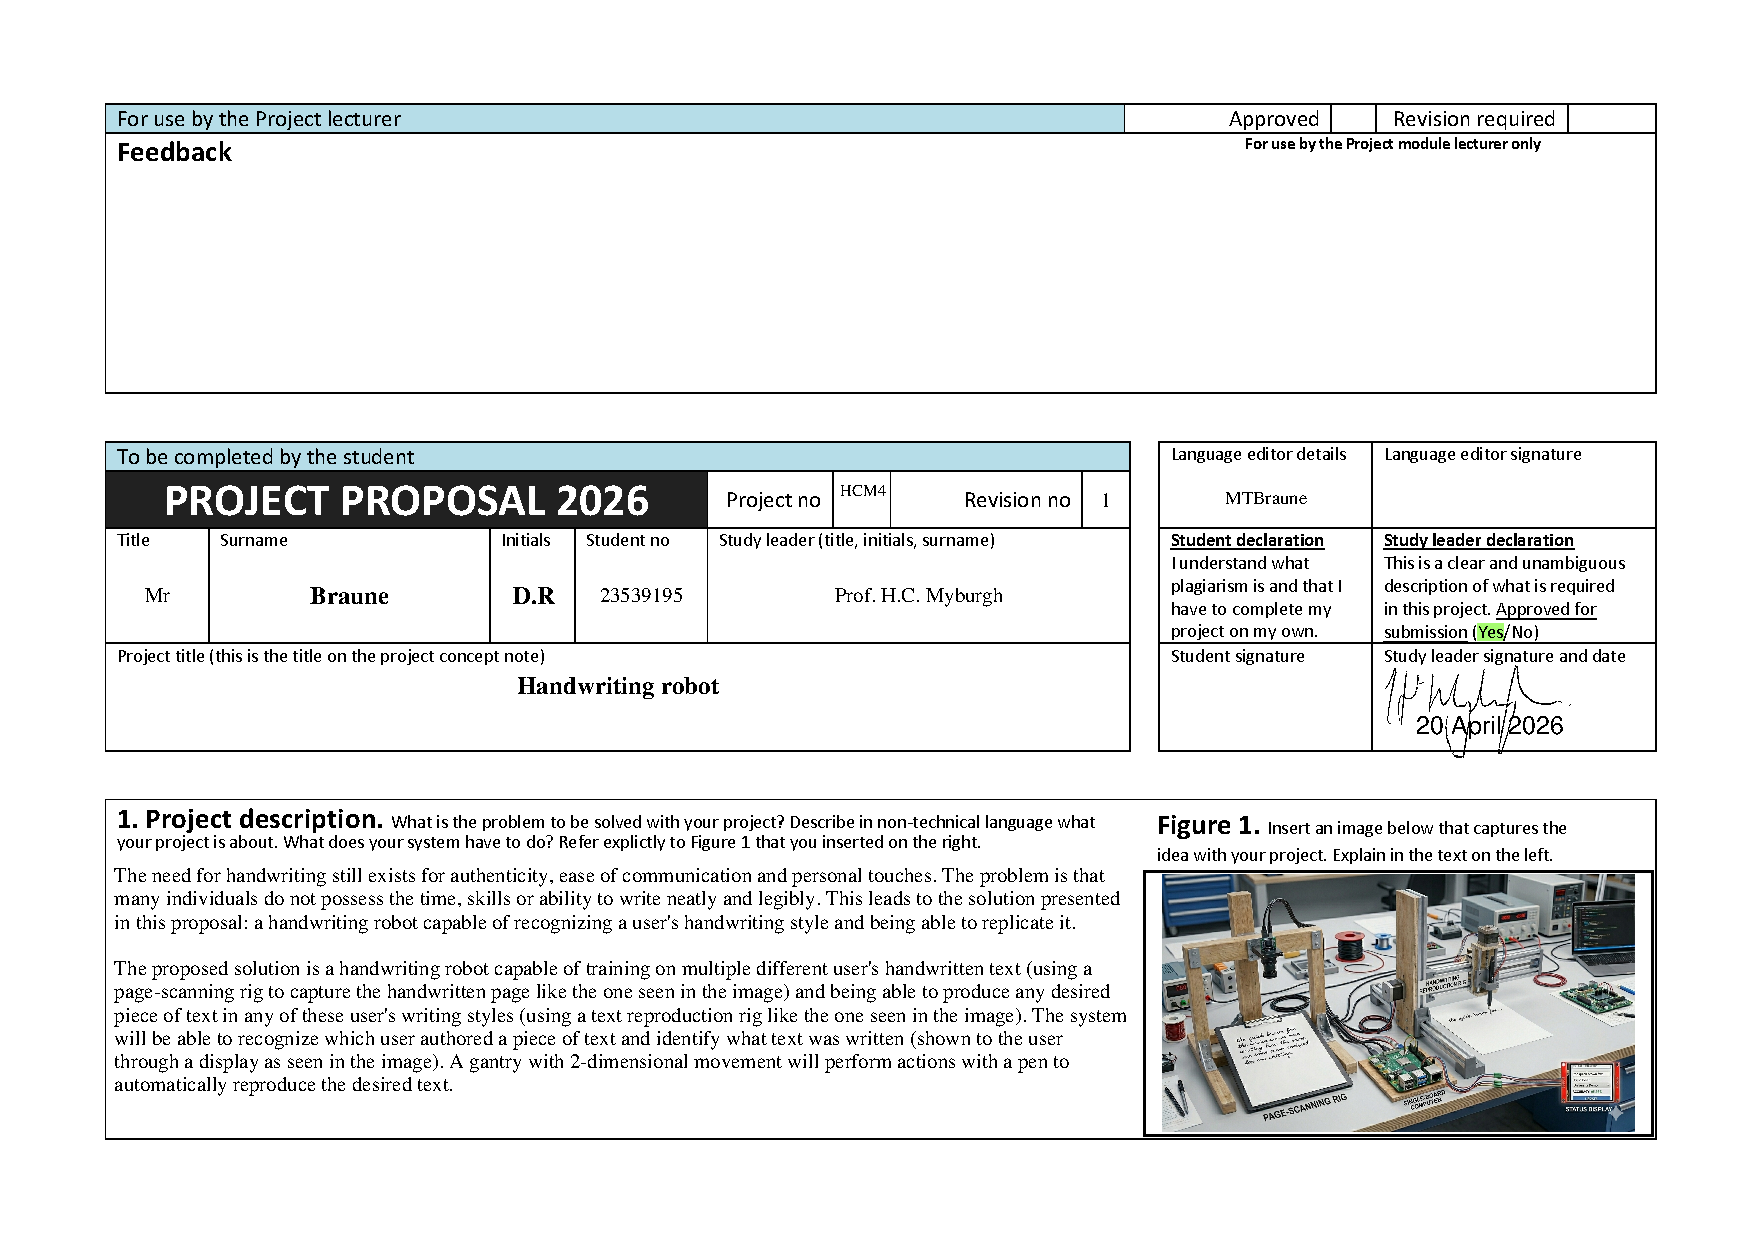
\includepdf[pages=-,landscape]{2_Project_Definition/project_proposal.pdf}


\eprsec{Part 3. Main Report}
\newpage

%% Reset the page number style and count.
\pagenumbering{arabic}
\setcounter{page}{1}

%% The abbreviation and notation lists in the Preamble are set as longtables and
%% silently consumed table numbers 1 and 2, so the first captioned table of the
%% report came out as "Table 3".  Appendix 4 requires figures and tables to be
%% numbered in separate sequences each starting at 1, so both counters are reset
%% here, at page 1 of Part 3.
\setcounter{table}{0}
\setcounter{figure}{0}

%% Import the main report content

\section{Literature study}
\label{sec:literature}
This section extends the first-semester literature study. Section~1.1 follows the signal path from photograph to robot; Section~1.2 states which technique was adopted for each subsystem and which requirement (R1 to R6) it serves.

\subsection{Background and context}
\label{sec:lit-background}

A handwriting-reproduction robot must solve three problems usually studied separately: \emph{reading}, \emph{writer identification} and \emph{writing} in a person's style with a machine.

\subsubsection{Handwriting recognition: problem, data and early solutions}
\label{sec:lit-hwr}

Handwriting recognition (HWR or HTR) converts handwriting into machine-readable text. Plamondon and Srihari~\cite{plamondon2000} distinguish \emph{online} recognition, where the pen position is recorded over time, from \emph{offline} work, where only an image of the finished writing exists. This project reads a photographed page, so it is the harder, offline problem~\cite{plamondon2000}. The distinction also matters for writing, because most pen-path generators are trained on online data (Section~\ref{sec:lit-synth}).

The data set fixes the \emph{unit of recognition}. EMNIST holds roughly 814\,000 isolated $28\times28$ characters~\cite{chen2023}, so models trained on it classify characters already cut out but cannot read connected writing. The IAM database of Marti and Bunke~\cite{marti2002} holds scanned pages of English sentences from many writers, labelled per line, which suits line recognisers and writer experiments.

Early offline systems followed a \emph{segment-then-classify} paradigm. LeCun \emph{et al.}~\cite{lecun1998} showed that a convolutional neural network (CNN) can classify isolated characters from pixels, and their LeNet-5 became the baseline for later character classifiers~\cite{chen2023,ji2021,yahya2021,mamun2024}. The weakness is segmentation: in cursive writing letters touch, and a wrong cut yields a fragment no classifier can label, so accuracy is bounded by the segmenter.

\subsubsection{Sequence recognition with neural networks}
\label{sec:lit-nn}

A \emph{convolutional layer} slides a kernel of learned weights over the image, so a stroke at a given angle is detected wherever it occurs~\cite{lecun1998}. Max-pooling halves the resolution, batch normalisation~\cite{ioffe2015} makes deeper networks trainable, and an optimiser such as Adam~\cite{kingma2015} applies the back-propagated gradients.

A CNN gives a fixed-size output, whereas a line has an unknown number of characters. The long short-term memory (LSTM) cell~\cite{hochreiter1997} gates a hidden state carried along the sequence, and a \emph{bidirectional} LSTM (BiLSTM) runs one in each direction, so each position uses the writing on both sides of it and resolves a stroke that could be a ``u'' or an ``n''.

The remaining difficulty is the training signal: the network emits $T$ time steps, but the label is only the transcription, so the alignment is unknown. Connectionist temporal classification (CTC)~\cite{graves2006} removes the need for it. Each step gives a distribution over the characters plus a ``blank''; a path $\pi$ assigns one symbol per step, and a collapse function $B$ merges repeats and deletes blanks. The probability of a text $Y$ given the image $X$ sums over all paths that collapse to it,
\begin{equation}
p(Y\mid X)=\sum_{\pi:\,B(\pi)=Y}\;\prod_{t=1}^{T}p_t(\pi_t\mid X),
\label{eq:lit-ctc}
\end{equation}
where $p_t(\pi_t\mid X)$ is the probability of symbol $\pi_t$ at step $t$. The loss is $-\ln p(Y\mid X)$, and the sum in Equation~\ref{eq:lit-ctc} and its gradient are computed by dynamic programming~\cite{graves2006}, so \emph{no character segmentation and no alignment labels are needed}. Decoding is greedy or lexicon-guided. Viterbi's algorithm~\cite{viterbi1967} instead aligns a \emph{known} transcription with the network output (forced alignment), used in Section~\ref{sec:lit-synth}.

Figure~\ref{fig:lit-ctc} shows both operations.

\begin{figure}[htbp]
\centering
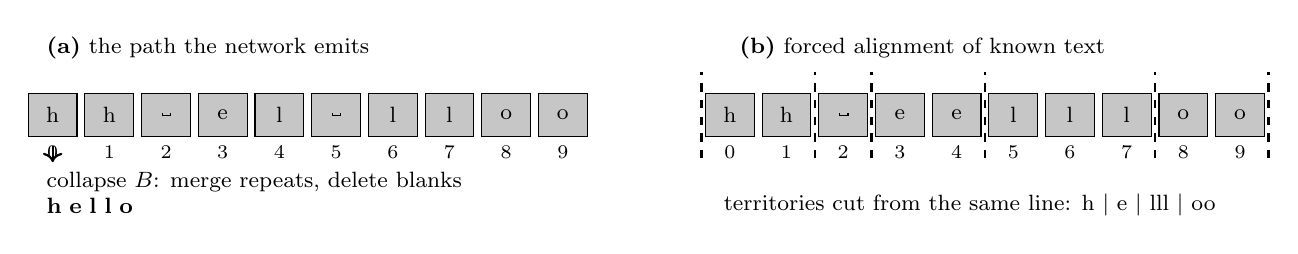
\begin{tikzpicture}[font=\footnotesize,
  cell/.style={draw,minimum width=6.2mm,minimum height=5.4mm,inner sep=0pt},
  blank/.style={cell,fill=gray!18},
  labl/.style={cell,fill=gray!45},
  brk/.style={draw,dashed,thick}]
% ---- left: emitted path -> collapse
\node[anchor=west] at (-0.2,3.35) {\textbf{(a)} the path the network emits};
\foreach \i/\s in {0/{h},1/{h},2/{\textvisiblespace},3/{e},4/{l},5/{\textvisiblespace},6/{l},7/{l},8/{o},9/{o}}{
  \ifx\s\textvisiblespace
    \node[blank] (a\i) at (\i*0.72,2.5) {\scriptsize$\varnothing$};
  \else
    \node[labl] (a\i) at (\i*0.72,2.5) {\s};
  \fi
}
\foreach \i in {0,...,9}{\node[font=\scriptsize,below] at (a\i.south) {\i};}
\node[anchor=west] at (-0.2,1.65) {collapse $B$: merge repeats, delete blanks};
\draw[->,thick] (0,2.1) -- (0,1.9);
\node[anchor=west] at (-0.2,1.35) {\textbf{h\;e\;l\;l\;o}};

% ---- right: known text -> forced alignment
\node[anchor=west] at (8.6,3.35) {\textbf{(b)} forced alignment of known text};
\foreach \i/\s in {0/{h},1/{h},2/{\textvisiblespace},3/{e},4/{e},5/{l},6/{l},7/{l},8/{o},9/{o}}{
  \ifx\s\textvisiblespace
    \node[blank] (b\i) at (8.6+\i*0.72,2.5) {\scriptsize$\varnothing$};
  \else
    \node[labl] (b\i) at (8.6+\i*0.72,2.5) {\s};
  \fi
}
\foreach \i in {0,...,9}{\node[font=\scriptsize,below] at (b\i.south) {\i};}
% character territories (blocks of steps assigned to one letter)
\draw[brk] (8.6-0.36,1.95) -- (8.6-0.36,3.05);
\draw[brk] (8.6+1*0.72+0.36,1.95) -- (8.6+1*0.72+0.36,3.05);
\draw[brk] (8.6+3*0.72-0.36,1.95) -- (8.6+3*0.72-0.36,3.05);
\draw[brk] (8.6+4*0.72+0.36,1.95) -- (8.6+4*0.72+0.36,3.05);
\draw[brk] (8.6+7*0.72+0.36,1.95) -- (8.6+7*0.72+0.36,3.05);
\draw[brk] (8.6+9*0.72+0.36,1.95) -- (8.6+9*0.72+0.36,3.05);
\node[anchor=west] at (8.6-0.2,1.35) {territories cut from the same line: h $\mid$ e $\mid$ lll $\mid$ oo};
\end{tikzpicture}
\caption{The two CTC operations used in this project. (a)~Collapsing the emitted path gives the transcription, so a line can be trained from its text alone with no character boundaries. (b)~Given the text, forced alignment finds the most probable block of time steps for each character; the dashed lines are the resulting territories, from which individual letter shapes are cut. Blank symbols are shaded.}
\label{fig:lit-ctc}
\end{figure}

Graves \emph{et al.}~\cite{graves2009} combined BiLSTM and CTC, reporting word accuracies of 74.1\,\% offline and 79.7\,\% online on IAM-derived data. Shi \emph{et al.}~\cite{shi2017} replaced the raw-pixel input by CNN features, naming the arrangement the convolutional recurrent neural network (CRNN). Puigcerver~\cite{puigcerver2017} showed on IAM that a CNN followed by BiLSTM layers matches costlier multidimensional recurrence, and the first-semester sources~\cite{ma2023,kumar2024,hemanth2022} agree.

\paragraph{Reported accuracies.}\label{sec:lit-acc} Quality is the character error rate (CER), the Levenshtein distance~\cite{levenshtein1966} between recognised and reference text divided by the reference length, or the word error rate (WER); this report uses character accuracy $1-\text{CER}$. Kizilirmak and Yanikoglu~\cite{kizilirmak2023}, whose CNN--BiLSTM--CTC network is closest to this one, report a best CER of 3.59\,\% and WER of 9.44\,\% on IAM, but only with lexicon-constrained decoding and test-time augmentation, so greedy decoding is worse. Word error rates run several times the CER because errors cluster inside words, and the accuracies above 95\,\% in the first-semester sources~\cite{yahya2021,ji2021,chen2023} are for isolated characters on clean data. Published work is also evaluated mostly on scanner images rather than on office photographs, which have uneven lighting, perspective, shadows and clutter, so pre-processing cannot be omitted.

\subsubsection{Image pre-processing and page segmentation}
\label{sec:lit-prep}

A photographed page must first become clean, separated line images; the first-semester sources~\cite{chen2023,hemanth2022} list normalisation, binarisation and line separation as standard.

A photograph records reflectance multiplied by lighting, so a lamp gradient or shadow changes the grey value of the paper itself, while \emph{binarisation} must decide for each pixel whether it is ink. Otsu's global method~\cite{otsu1979} picks the threshold $t^{*}$ maximising the between-class variance,
\begin{equation}
t^{*}=\arg\max_{t}\;\omega_{B}(t)\,\omega_{F}(t)\,\bigl[\mu_{B}(t)-\mu_{F}(t)\bigr]^{2},
\label{eq:lit-otsu}
\end{equation}
In Equation~\ref{eq:lit-otsu}, $\omega_B(t)$ and $\omega_F(t)$ are the fractions of pixels at or below, and above, $t$, with mean grey values $\mu_B(t)$ and $\mu_F(t)$. It needs no tuning but fails under uneven lighting, dropping strokes in dim areas or reading shadows as ink. \emph{Adaptive} methods threshold each pixel against a local mean and standard deviation~\cite{sauvola2000} or an integral image~\cite{bradley2007}; flat-field correction, dividing the image by a blurred copy of itself, flattens a multiplicative gradient. The summed-area table of Crow~\cite{crow1984} makes local means cheap, any rectangle sum needing four look-ups.

Ink pixels are grouped into \emph{connected components} by the two-pass labelling of Rosenfeld and Pfaltz~\cite{rosenfeld1966}; their heights give a typical character height, so thresholds in character heights are independent of camera resolution and handwriting size. Skew is found by rotating through trial angles and keeping the most sharply peaked row-wise ink histogram, the projection-profile method of Postl~\cite{postl1986} \mustdo{confirm the exact title and page range of the Postl 1986 ICPR reference, or replace it with Baird 1987 if that is the source preferred; the page range was left out of the bibliography rather than guessed.}. Lines come from gaps in that profile, which assumes straight lines, or from chaining neighbouring components, which tolerates drifting baselines and diagrams. Printed ruling lines glue letters together and must be removed without deleting the strokes crossing them. These steps are described for scanned documents rather than for a camera, desk background, ruled paper and diagrams together.

\subsubsection{Writer identification and style}
\label{sec:lit-writer}

Writer identification asks which member of a known set wrote a sample. The proposal grounded its target in the signature classification of Agduk and Aydemir~\cite{agduk2022}, who compared transfer-learning CNNs; signatures are short and practised, whereas this system must identify the writer of running text while reading it. Bulacu and Schomaker~\cite{bulacu2007} are \emph{text independent}, comparing histograms of contour direction and curvature against those of characteristic letter shapes; slant, x-height, stroke width, spacing and joined-letter frequency also describe style. A CNN can instead be trained on the images: FragNet~\cite{he2020} classifies small fragments and pools the evidence.

Two cautions affect the project. A classifier trained on ink can rely on cues a machine cannot reproduce: stroke thickness and ink density follow the writer's pen and pressure, whereas a robot draws at constant width. Most of this work uses hundreds of writers, whereas this closed set of thirteen has about one and a half thousand text lines, and test partitions that share pages with training data inflate accuracy.

\subsubsection{Handwriting synthesis and pen-path generation}
\label{sec:lit-synth}

\emph{Neural sequence generators} are trained on recorded pen trajectories: Graves~\cite{graves2013} conditioned an LSTM on the text through a soft attention window to predict the next pen offset and pen-up probability, which needs hundreds to thousands of recorded lines that photographs of a few pages cannot supply. Pretrained image generators such as the generative adversarial network of Kang \emph{et al.}~\cite{kang2020} need less data per writer, but produce rasters and give no control of slant, size or spacing. \emph{Exemplar} (glyph-based) methods are the alternative: Haines \emph{et al.}~\cite{haines2016} assemble glyphs from an annotated sample with learned spacing, thickness and pressure, so a few pages per writer suffice and the letterforms are the writer's own. Forced alignment of the transcription with a recogniser's output (Section~\ref{sec:lit-nn}) extracts those glyphs without hand-drawn boundaries.

\emph{Thinning} reduces a stroke to a one-pixel centre line without breaking connectivity; Zhang and Suen~\cite{zhang1984} delete boundary pixels in two alternating sub-iterations. The Douglas--Peucker algorithm~\cite{douglas1973} then simplifies the traced line, recursively keeping the point farthest from the chord while its distance exceeds a tolerance $\varepsilon$; the first-semester report noted it is not guaranteed optimal.

\subsubsection{Robotic writing and linear motion}
\label{sec:lit-robot}

The first-semester study identified three robot topologies~\cite{teikari2016}. A \emph{Cartesian} (gantry) system moves along two perpendicular linear axes: it is simple, its kinematics are the identity and it covers a flat page naturally. \emph{Serial-chain} arms reach further but need inverse kinematics and accumulate joint errors; \emph{parallel} robots are stiff and precise but have a small workspace. Belt, rack-and-pinion and ball-screw actuators are used in handwriting systems for durability and low cost~\cite{acarnley2002}.

Most such systems use stepper motors, which turn by a fixed angle for every pulse; a driver converts the pulse (STEP) and direction level (DIR) into winding currents, and microstepping gives finer positions. Acarnley~\cite{acarnley2002} treats open-loop stepping, torque--speed limits and controlled acceleration to avoid lost steps. Because position follows from counting pulses, error does not accumulate if commanded positions become integer step counts from a known reference. Bresenham's algorithm~\cite{bresenham1965}, from digital plotters, interleaves the two axes of a line in integer arithmetic, an error accumulator deciding when the slower axis steps, so the deviation never exceeds one step.

The proposal used Teikari's analysis~\cite{teikari2016} to set about four seconds per character, the 0.3\,mm gantry error of Huang and Xiong~\cite{huang2024} as the basis of the 0.5\,mm limit of R5, and the roughly 85\,\% accuracy derived from Babushkin \emph{et al.}~\cite{babushkin2025} for R1. None shows how a robot would reproduce an \emph{identified} person's style from a photograph.

\subsubsection{Embedded deployment and shortcomings of the literature}
\label{sec:lit-embedded}

Executing all processing on a single-board computer (SBC) makes every algorithm's cost matter. Sze \emph{et al.}~\cite{sze2017} stress that multiply--accumulate operations and the memory for weights and activations determine time and energy on a constrained processor, and that convolutions dominate. Most research relies on large frameworks, so the algorithms are never exposed~\cite{chen2023}.

Four shortcomings follow. First, recognition, writer identification, synthesis and robotics are studied in isolation, with no complete system from a photographed page to a drawn one. Second, embedded deployment is rarely demonstrated, and then through frameworks. Third, reported accuracies depend on benchmark conditions (lexicon, scanner images, shared writers or pages) unlike a photograph. Fourth, the generation literature needs recorded trajectories or large pre-training and evaluates output as an image, whereas this project must evaluate output a machine can draw with a constant-width pen.

\subsection{Application of the background to this project}
\label{sec:lit-application}

\subsubsection{Reading and identification (R2, R4)}

Cursive writing cannot be segmented reliably and the labels are line transcriptions, so a line-level recogniser trained with CTC~\cite{graves2006} was adopted and FU\,2.2 (character separation) became separation into \emph{lines}.
The architecture follows the CNN--BiLSTM--CTC pattern~\cite{shi2017,puigcerver2017,kizilirmak2023} with about 3.36 million parameters; decoding is greedy, because lexicon decoding needs corpora the project does not have (Sections~\ref{sec:textrec} and~\ref{sec:results}).
For writer identification a learned CNN on text lines was chosen over hand-crafted statistics~\cite{bulacu2007} or fragment pooling~\cite{he2020}, since the recogniser's features could be reused and accuracy measured directly.
Following Section~\ref{sec:lit-writer}, two classifiers of the same architecture were built: one on real photographed ink, one on lines thinned and redrawn at constant width, which removes thickness and pressure cues and matches the gantry.
The second was needed because the first, almost perfect on real handwriting, identified only 28\,\% of the machine's drawn lines (Section~\ref{sec:writerid}).
Both are closed-set decisions: they address R2 and the storage requirement of R6 but cannot report an unknown writer (Section~\ref{sec:dis-failure}).

\subsubsection{Reproduction (R1, R3, R5, R6)}

Neural generators need pen recordings the project does not have, and image generators produce rasters without parametric control, so an exemplar approach after Haines \emph{et al.}~\cite{haines2016} was adopted.
Glyphs are harvested from each writer's pages: the recogniser aligns the known transcription with the line (Figure~\ref{fig:lit-ctc}b), the ink is cut into letter territories, thinned~\cite{zhang1984}, traced, simplified~\cite{douglas1973}, normalised to the x-height and de-slanted; the glyphs and style statistics form a \emph{style profile} stored as a file.
Synthesis places glyphs with the writer's slant, spacing and random variation; the best of several candidates is kept by a combined score of legibility and writer-classifier confidence.
The scoring networks also perform the selection and so cannot be an independent verdict (Sections~\ref{sec:synthesis} and~\ref{sec:results}).

A Cartesian gantry with stepper motors was adopted, since position follows from step counts, the only practical route to 0.5\,mm without position sensors.
Pen paths in millimetres become G-code, which a program converts to absolute integer step counts, interleaving the axes with Bresenham's algorithm~\cite{bresenham1965} and reading the limit switches before every step; the step resolution is 12.5\,$\mu$m against the 0.5\,mm limit of R5 (Section~\ref{sec:gantry}).
Resolution is not accuracy: belt stretch, backlash, home-switch repeatability and pen compliance determine the true error, and none was measured, so R5 remains unassessed in Section~\ref{sec:results}.

\subsubsection{Embedded execution and the contribution}

Following Sze \emph{et al.}~\cite{sze2017}, the networks' cost was analysed: about $4.2\times10^{9}$ multiply--accumulate operations and 13.4\,MB of weights per recogniser pass, 91\,\% of the arithmetic being convolution.
Inference of both networks was therefore written from first principles in Python, without a neural-network framework, and agrees with the training implementation to about $10^{-5}$ in log-probability (Section~\ref{sec:textrec}).
Recognition met the 25\,ms allowance of R4 at 8.86\,ms per character, but page segmentation took 35 to 57\,s against the roughly 2\,s the requirement leaves, so R4 fails on segmentation rather than on the network (Section~\ref{sec:results}).
The contribution is therefore a complete pipeline from photograph to pen strokes, implemented from first principles in one language.

\newpage

\section{Approach}
\label{sec:approach}
This section explains how the functional analysis of the approved proposal became a first concept; mathematics and parameter values are deferred to Section~3.

\subsection{From functional analysis to concept}
\label{sec:app-concept}

The proposal defined three modes (training, classification and reproduction) and four functional units: page scanning (FU\,1), the single-board computer (SBC) and its eight processing steps (FU\,2), the gantry (FU\,3) and the power supply (FU\,4). Requirements R1 to R6 and two field conditions, FC1 (a well-lit room, 400 to 1000\,lux) and FC2 (a stable, level, vibration-free surface), were attached to this structure.

The first concept kept this structure and made one decision per block (Figure~\ref{fig:app-concept}); Table~\ref{tab:app-fu} gives each unit's realisation and its departures, justified in Section~\ref{sec:app-alternatives}.

\begin{figure}[htbp]
\centering
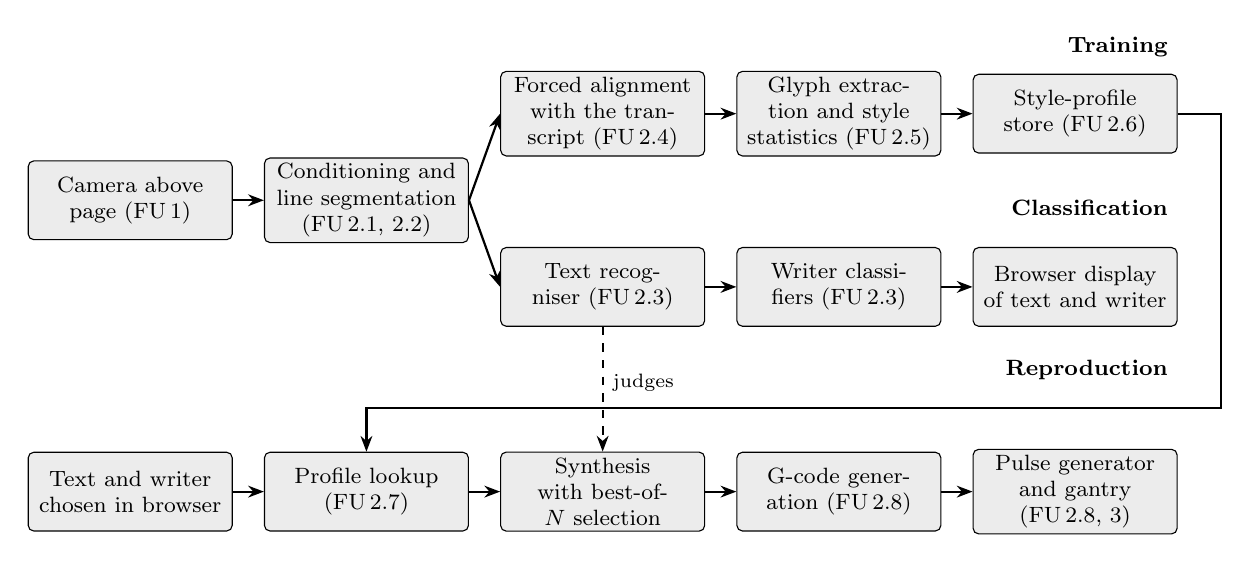
\begin{tikzpicture}[
  blk/.style={draw,rounded corners=2pt,fill=gray!15,minimum height=1.0cm,text width=2.45cm,align=center,font=\footnotesize,inner sep=2pt},
  arr/.style={-{Stealth[length=2mm]},thick},
  darr/.style={-{Stealth[length=2mm]},thick,dashed},
  lab/.style={font=\footnotesize\bfseries,anchor=east}]
\node[blk] (cam) at (0,-1.1) {Camera above page (FU\,1)};
\node[blk] (seg) at (3,-1.1) {Conditioning and line segmentation (FU\,2.1, 2.2)};
\node[blk] (ali) at (6,0) {Forced alignment with the transcript (FU\,2.4)};
\node[blk] (gly) at (9,0) {Glyph extraction and style statistics (FU\,2.5)};
\node[blk] (sto) at (12,0) {Style-profile store (FU\,2.6)};
\node[blk] (rec) at (6,-2.2) {Text recogniser (FU\,2.3)};
\node[blk] (wid) at (9,-2.2) {Writer classifiers (FU\,2.3)};
\node[blk] (dis) at (12,-2.2) {Browser display of text and writer};
\node[blk] (inp) at (0,-4.8) {Text and writer chosen in browser};
\node[blk] (lkp) at (3,-4.8) {Profile lookup (FU\,2.7)};
\node[blk] (syn) at (6,-4.8) {Synthesis with best-of-$N$ selection};
\node[blk] (gco) at (9,-4.8) {G-code generation (FU\,2.8)};
\node[blk] (gan) at (12,-4.8) {Pulse generator and gantry (FU\,2.8, 3)};
\draw[arr] (cam)--(seg);
\draw[arr] (seg.east)--(ali.west);
\draw[arr] (ali)--(gly); \draw[arr] (gly)--(sto);
\draw[arr] (seg.east)--(rec.west);
\draw[arr] (rec)--(wid); \draw[arr] (wid)--(dis);
\draw[arr] (inp)--(lkp); \draw[arr] (lkp)--(syn); \draw[arr] (syn)--(gco); \draw[arr] (gco)--(gan);
\draw[arr] (sto.east) -- ++(0.55,0) |- ($(lkp.north)+(0,0.55)$) -- (lkp.north);
\draw[darr] (rec.south) -- node[right,font=\scriptsize,pos=0.45]{judges} (syn.north);
\node[lab] at (13.3,0.85) {Training};
\node[lab] at (13.3,-1.2) {Classification};
\node[lab] at (13.3,-3.25) {Reproduction};
\end{tikzpicture}
\caption{Block diagram of the chosen concept. Solid arrows show the flow of data; the dashed arrow shows that the recogniser and writer classifier also judge the candidates in the synthesis block. Functional-unit numbers of the proposal are in brackets. Training is performed offline and is not part of the browser interface.}
\label{fig:app-concept}
\end{figure}

\begin{table}[htbp]
\centering
\fontsize{9}{10.5}\selectfont
\begin{tabularx}{\linewidth}{|p{1.5cm}|X|X|}
\hline
\textbf{Unit} & \textbf{Realisation in the final concept} & \textbf{Departure from the proposal} \\
\hline
FU\,1, 2.1 & Camera on a fixed rig over an A4 page; photograph conditioned for scale, lighting, binarisation, skew and ruled lines. & None; conditioning is far more extensive than anticipated. \\
\hline
FU\,2.2 & Separation of the page into \emph{text lines}. & Lines instead of characters (Section~\ref{sec:app-alternatives}). \\
\hline
FU\,2.3, 2.4 & Line recogniser for text, two classifiers for the writer; gradient-based training offline. & Text and writer by separate networks; training not in the interface. \mustdo{state on which computer the networks were trained and the profiles built; the proposal requires embedded-only processing.} \\
\hline
FU\,2.5--2.7 & A style profile per writer (pen-path glyphs and style statistics) stored as a data file and loaded at start-up. & Stored per glyph variant with statistics, not one map per character. \\
\hline
FU\,2.8, 3.1, 3.2 & G-code, then step/direction pulses from the SBC to two stepper-driver modules; limit switches bound the travel. & Two stages; limit switches added as a safety function. \\
\hline
FU\,3.3, 3.4 & Pen and paper holders; pen lifted by a one-way toggle gear motor with a position switch. & Pen lift not controlled through the stepper driver. \mustdo{reason for this change.} \\
\hline
FU\,4 & Power supply. & \mustdo{supply voltages, current ratings and distribution.} \\
\hline
\end{tabularx}
\caption{Translation of the functional units of the proposal into the first concept.}
\label{tab:app-fu}
\end{table}

\subsection{Design alternatives and trade-offs}

\begin{table}[htbp]
\centering
\fontsize{9}{10.5}\selectfont
\begin{tabular}{|p{1.6cm}|p{3.4cm}|p{4.3cm}|p{4.3cm}|}
\hline
\textbf{Decision} & \textbf{Alternatives} & \textbf{Comparison} & \textbf{Preferred and reason} \\
\hline
Unit of recognition & (a) Cut characters, classify each. (b) Cut lines, read with a sequence recogniser. & (a) Needs a segmenter for joined letters and character-level labels (absent); cannot repair a wrong cut. (b) No boundaries below the line; uses context; larger network. & (b): cursive cannot be segmented reliably, labels exist per line, and segmenter errors would bound system accuracy. \\
\hline
Networks for text and writer & (a) One network, two outputs. (b) Separate networks. & (a) One computation, but the tasks compete. (b) Each trainable and measurable alone. & (b): an early joint network learned the writer quickly while text accuracy stayed very low (training-script documentation; log not kept). \\
\hline
Synthesis of writing & (a) Neural generator on pen trajectories. (b) Pretrained image generators. (c) Library of the writer's own glyphs. & (a) Needs recorded pen trajectories (unavailable). (b) Raster output, no control of size or slant, slow without a graphics processor. (c) About nine pages per writer, strokes with controllable parameters; cursive links partly lost. & (c): a from-scratch generator trained on stroke data from the photographs learned slant and roundness but not legible letters; image generators took tens of seconds per line on a processor-only computer. \\
\hline
Selection of output & (a) Use the first result. (b) Draw $N$ candidates, keep the best by recogniser and writer classifier jointly. & (a) Fastest, but random variation gives good and bad results. (b) Time grows with $N$. & (b): in a design-stage tuning run at $N=14$, writer identification of the synthesised output rose from 79.2\,\% to 97.5\,\% and character accuracy from 75.9\,\% to 81.6\,\%. The later official evaluation at $N=30$ did not reproduce that writer-identification figure, measuring 80.1\,\% directly and 89.7\,\% through the G-code path (Section~\ref{sec:results}); the 97.5\,\% should therefore be read as a tuning observation on a smaller sentence set, not as a result. In both cases the judges also select the candidate, so neither is independent evidence. \\
\hline
Location of processing & (a) Offload to a personal computer. (b) All inference on the SBC. & (a) Faster, but contradicts the proposal. (b) Limits memory, compute and methods. & (b), as required; method cost was considered throughout (Section~\ref{sec:lit-embedded}). \\
\hline
\end{tabular}
\caption{Software design decisions, alternatives and reasons for the preferred solution.}
\label{tab:app-software}
\end{table}

\begin{table}[htbp]
\centering
\fontsize{9}{10.5}\selectfont
\begin{tabular}{|p{1.6cm}|p{3.4cm}|p{4.3cm}|p{4.3cm}|}
\hline
\textbf{Decision} & \textbf{Alternatives} & \textbf{Comparison} & \textbf{Preferred and reason} \\
\hline
Page capture & (a) Fixed camera. (b) Flatbed scanner. & (a) Instant capture, standard interface, live framing; lighting and tilt handled in software (FC1 applies). (b) Even lighting; larger separate device with a scanning delay. & (a): suits the compact rig and the capture budget of R4; cost is the extensive conditioning of Section~\ref{sec:segmentation}. \\
\hline
Robot type & (a) Cartesian gantry. (b) Serial arm. (c) Parallel robot. & (a) Identity kinematics, flat page, axis errors do not add up. (b) Inverse kinematics, joint errors add up. (c) Stiff, but small workspace, complex kinematics. & (a): position follows from step counts; the 0.5\,mm limit of R5 is simplest to meet and verify~\cite{teikari2016}. \\
\hline
Motor control & (a) Separate microcontroller receives moves. (b) SBC generates STEP/DIR pulses. & (a) Offloads timing, but an issued move cannot be stopped without a round trip. (b) Less deterministic timing; limit switches read before every step. & (b): stopping within one step on a limit-switch trip was valued above deterministic timing. \\
\hline
\end{tabular}
\caption{Hardware design decisions, alternatives and reasons for the preferred solution.}
\label{tab:app-hardware}
\end{table}

\label{sec:app-alternatives}

Each major decision was weighed against criteria from the requirements: accuracy (R1, R2), processing time on the SBC (R3, R4), the data available for thirteen writers (R6), first-principles implementation, and mechanical and electrical simplicity and safety. Tables~\ref{tab:app-software} and~\ref{tab:app-hardware} of the Appendix list the processing-chain and physical-system decisions with their alternatives and the reason for each choice, argued in full in Section~\ref{sec:design}.

Training from line transcriptions with connectionist temporal classification~\cite{graves2006} costs a larger network and a heavy dependence on robust \emph{line} segmentation, and the glyph library's weak case, recognised from the outset, is the heavily cursive hand, whose letter links are lost when letters are cut apart.

\subsection{Off-the-shelf components and own design}
\label{sec:app-offshelf}

Consistent with rows 5 and 6 of the proposal's requirement tables, the camera, the SBC (an ODROID N2+), the stepper motors and driver modules, the limit switches, the pen, standard gantry parts, storage and the power supply were bought, with standard system drivers for camera and input/output access. The student designed the image conditioning and page segmentation, the two networks and their training, the style-profile builder, synthesiser and candidate selection, the G-code and step-pulse conversions with their safety checks, the gantry calibration, the browser interface and the gantry's mechanical parts in CAD. \mustdo{list of the mechanical parts designed and manufactured, as opposed to purchased.}

\subsection{Verification strategy and roadmap}
\label{sec:app-verification}

The design was verified against two kinds of evidence: performance on data \emph{held out} from training, and the proposal's \emph{measurable specifications} of character and style accuracy (R1), text and writer accuracy (R2), time per character (R3, R4), positional error (R5) and stored styles (R6). The held-out data are a public line-level partition for the recogniser and one whole page per public-data writer for the classifiers; that for the two personal writers is weaker, since its lines come from the training pages, as stated where its figures are quoted. Synthesis was tuned and judged by the same two networks, so its figures measure agreement with those judges, and R3 to R5 need measurements on the built hardware; Section~4 reports what was and was not measured.

Section~3 follows the path of the data, because each stage uses the output of the preceding one, from the architecture (Section~\ref{sec:blockdiagram}) and page conditioning (Section~\ref{sec:segmentation}), where FC1 and FC2 act, to the gantry (Section~\ref{sec:gantry}) and integration (Section~\ref{sec:system}); R1 comes last because it rests on everything upstream.

\newpage

\section{Design and implementation}
\label{sec:design}

% ---- Writer 2 shared definitions (used by 3.1 - 3.5) ----
\providecommand{\wht}{h_{\mathrm{t}}}
\tikzset{
  w2box/.style={draw,rounded corners=2pt,fill=gray!12,align=center,font=\footnotesize,minimum height=7mm,inner sep=3pt},
  w2dark/.style={draw,rounded corners=2pt,fill=gray!30,align=center,font=\footnotesize,minimum height=7mm,inner sep=3pt},
  w2store/.style={draw,fill=white,align=center,font=\footnotesize,minimum height=7mm,inner sep=3pt,double,double distance=1pt},
  w2io/.style={draw,rounded corners=6pt,fill=white,align=center,font=\footnotesize,minimum height=7mm,inner sep=3pt},
  w2arr/.style={-{Stealth[length=2.2mm]},thick},
  w2dash/.style={-{Stealth[length=2.2mm]},thick,dashed},
  w2group/.style={draw,dashed,rounded corners=4pt,inner sep=5pt},
  w2lab/.style={font=\scriptsize,inner sep=1.5pt}
}

\subsection{Design summary}
\label{sec:summary}

This section summarises the project design tasks and how they were implemented (see Tables~\ref{tab:des-summary} and~\ref{tab:des-summary2}).
The rows follow the deliverables of line~5 of the table of Section~4 of the approved project proposal (requirements R1 to R6, ``own design contribution'') and the nine design and implementation tasks of Section~6.1 of that proposal.
The summary is given as two tables only so that neither of them runs across a page break; together they are the single design summary that the report requires, and the column headings are the same in both.
A task is marked \emph{Completed} only when the deliverable itself works; where any part of it is missing, unbuilt or unmeasured it is marked \emph{Incomplete} and the second column says exactly what is missing.
R1 is reproduction of text in the style of any writer of the training set, R2 decoding of the text and identification of the writer, R3 reproduction speed, R4 classification time, R5 gantry positional accuracy and R6 at least ten stored writing styles.
Only work designed and implemented by the student is claimed; the physical parts that were bought as finished items (camera, single-board computer, stepper motors and driver modules, pen, end-stop switches, power supply, standard mechanical parts) carry no design credit.
All image-processing, machine-learning, trajectory and motion-control algorithms were written by the student in Python, and the only external functions used interface with the camera, the file system and the network.

Two deviations from the proposal shape several rows.
First, the proposal planned an explicit separation of the page into characters (functional unit (FU) 2.2) before classification; the implemented design separates the page into \emph{text lines} only and reads each line with a sequence recogniser, because the characters of connected handwriting have no reliable boundaries and a segmentation error would pass directly into a wrong reading (Sections~\ref{sec:segmentation} and~\ref{sec:textrec}).
Second, the proposal placed training and the building of trajectory maps on the single-board computer (FU 2.4 to 2.6); in the implemented system the networks and the per-writer style profiles are produced by offline programs on a general-purpose computer, and only inference, synthesis and motion control run on the single-board computer, so the training mode is not offered by the user interface.
\mustdo{state the computer used for network training (the project notes mention a laptop processor and a cloud notebook) and confirm that the single-board computer was not used for training.}

\begin{table}[!htbp]
\centering
\fontsize{8}{9.4}\selectfont
\setlength{\tabcolsep}{3pt}
\renewcommand{\arraystretch}{1.0}
\begin{tabular}{|p{3.1cm}|p{7.4cm}|p{3.7cm}|}
\hline
\textbf{Deliverable or task} & \textbf{Implementation} & \textbf{Completion of deliverable or task, and section in the report} \\
\hline
Research of network types, structure, layers and feature extraction (task 6.1.1) &
A literature study of convolutional, recurrent and sequence-to-sequence recognisers, of writer-identification methods and of the alternatives to each, used to choose the methods of Sections~\ref{sec:textrec} and~\ref{sec:writerid}. &
Completed. Section~\ref{sec:literature}. \\
\hline
Research of conditioning, noise removal, separation and trajectory mapping (task 6.1.2) &
A literature study of thresholding, illumination correction, line and character separation, thinning and exemplar-based handwriting synthesis, used to choose the methods of Sections~\ref{sec:segmentation} and~\ref{sec:styleprofile}. &
Completed. Section~\ref{sec:literature}. \\
\hline
Image conditioning and noise removal (FU 2.1; R2, R4) &
Designed and implemented from first principles using only array arithmetic: size normalisation, page localisation, flat-field illumination correction with summed-area tables, local adaptive thresholding, skew correction and removal of printed rules, faint print and neighbouring-page ink. &
Completed. Section~\ref{sec:segmentation}. \\
\hline
Separation into characters (FU 2.2; R2, R4) &
Implemented as separation into text lines and diagram regions rather than into characters (connected components, glyph-scale estimation, chaining, baseline merging, text versus non-text scoring, one deskewed crop per line). Character territories are derived only offline, by forced alignment, when style profiles are built. The reason for the change from the proposal is given above and in Section~\ref{sec:textrec}. &
Completed. Sections~\ref{sec:segmentation}, \ref{sec:textrec}. \\
\hline
Optimised and efficient character separation (R4; task 6.1.3) &
The segmentation was profiled and its two dominant routines, component labelling and the box sums, were rewritten in C by the student at 84 to 88\% faster each, 25 to 32\% faster per page. The C routines are not called by the deployed program, and segmentation still exceeds the R4 allowance by over an order of magnitude. &
Incomplete. Sections~\ref{sec:segmentation}, \ref{sec:results}. \\
\hline
Neural network that decodes the text (FU 2.3; R2) &
Convolutional and bidirectional recurrent network with connectionist temporal classification (CTC) output, 3\,358\,763 trainable parameters. The layer pattern follows a published design~\cite{kizilirmak2023}; the student chose the input geometry, data pipeline, label cleaning, augmentation and staged training, and wrote the from-scratch module (forward and backward passes, optimisers, no machine-learning library) used by training, validation and deployment alike. &
Completed. Section~\ref{sec:textrec}; measured accuracy 98.61\% character and 94.21\% word on 669 real line crops (Section~\ref{sec:results}). \\
\hline
Neural network that identifies the writer (FU 2.3; R2) &
Two thirteen-class convolutional classifiers sharing the recogniser's backbone and layer module: an ink-based one for photographs, which reached 99.78\% over 1358 real lines, and one whose input is re-drawn at a constant pen width by the student's stroke normalisation, with page-level aggregation. &
Completed. Section~\ref{sec:writerid}; measured accuracy 93.67\% for the normalised classifier after a training fault was corrected (Section~\ref{sec:results}). \\
\hline
Training on datasets and choice of layer numbers (FU 2.4; task 6.1.4) &
Training programs for the recogniser and both classifiers on a public database, a public line-level set and the photographed personal pages, all built on the from-scratch module of Section~\ref{sec:textrec-numpynn}, whose every layer gradient was checked against numerical differentiation in 78 configurations. A sweep over widths, depths and learning rates was programmed but no result was kept, so the layer numbers are the published design's and are not justified by this project's own measurement. Training is offline. &
Incomplete. Sections~\ref{sec:textrec}, \ref{sec:writerid}. \\
\hline
Trajectory maps and permanent storage (FU 2.5 to 2.7; R1, R6) &
Letter shapes are harvested by forced alignment with the recogniser, thinned to centre-line pen paths, normalised and stored as one JavaScript Object Notation (JSON) file per writer with measured style statistics; thirteen styles exist, for eight database writers and five personal writers. The builder is an offline program. &
Completed. Section~\ref{sec:styleprofile}. \\
\hline
Pen trajectory mapping and G-code (FU 2.5 to 2.8; R1, R3) &
A synthesiser assembles the writer's own letter paths into lines (slant, spacing, joins, wobble) with a best-of-$N$ search judged by the recogniser and the writer classifier; a generator turns the trajectory into G-code, the numerical-control command language of plotters, with placement, stroke ordering and pen-state tracking, and a simulator replays it. &
Completed. Sections~\ref{sec:synthesis}, \ref{sec:gcode}. \\
\hline
Optimisation of pen movement (R3) &
Greedy nearest-endpoint stroke ordering reduces pen-up travel. The saving it achieves was not measured. &
Completed. Section~\ref{sec:gcode}. \\
\hline
\end{tabular}
\caption{Design summary, part 1 of 2: the research, image-processing, network and trajectory tasks.}
\label{tab:des-summary}
\end{table}

\begin{table}[!htbp]
\centering
\fontsize{8}{9.4}\selectfont
\setlength{\tabcolsep}{3pt}
\renewcommand{\arraystretch}{1.0}
\begin{tabular}{|p{3.1cm}|p{7.4cm}|p{3.7cm}|}
\hline
\textbf{Deliverable or task} & \textbf{Implementation} & \textbf{Completion of deliverable or task, and section in the report} \\
\hline
Capture rig and deployment on the single-board computer (FU 1; R2, R4; task 6.1.5) &
A generic USB camera in a printed housing that clamps the page flat, read with a live preview and a five-frame warm-up; the recognition, synthesis and motion programs run on the ODROID N2+ behind a web server. The rig geometry, camera resolution and lighting are not documented. \mustdo{camera model, resolution, mounting height, field of view, lamp, lux readings, photograph of the rig.} &
Incomplete. Sections~\ref{sec:blockdiagram}, \ref{sec:system}. \\
\hline
Testing the classifier on the single-board computer with captured images (task 6.1.6) &
The deployed programs were written to run on the board and do run on it, but no accuracy or timing figure in this report was obtained on the board; every measurement reported in Section~\ref{sec:results} was taken on a laptop. &
Incomplete. Section~\ref{sec:results}. \\
\hline
Gantry design and construction in CAD (FU 3.3, 3.4; R5; task 6.1.7) &
A Cartesian X/Y gantry built by the student from bought parts: one motor turning an 8\,mm cross-shaft that drives both ends of the moving bridge, and a second motor on that bridge driving the carriage, both on GT2 belts over linear bearings and chromed rods, with four end-stops. Hand-measured travel 204\,mm (X) and 262\,mm (Y). The machine exists but no CAD drawing or photograph was kept. \mustdo{CAD files and photographs.} &
Incomplete. Section~\ref{sec:gantry}. \\
\hline
Pen holder, pen adjuster and paper holder (R5) &
The pen is carried on the moving carriage in a holder with the toggle cam of the lift mechanism above it, and the page is clamped flat in the camera housing for capture. Whether the holder provides a pen-height adjustment, and how the paper is held on the writing bed, are not recorded. \mustdo{confirm how the pen height is adjusted and how the paper is held down on the writing bed, and supply a photograph of each; neither is documented in the project files.} &
Incomplete. Section~\ref{sec:gantry}. \\
\hline
Power supply (FU 4) &
A 24\,V supply feeds both stepper drivers through a 100\,\textmu F bulk capacitor. The conversion to the voltages the single-board computer and the pen motor require is not documented, no power budget was drawn up and the supply's rating is unknown. &
Incomplete. Section~\ref{sec:gan-supply}. \\
\hline
Stepper-motor control and pen lift (FU 2.8, 3.1 to 3.4; R5; task 6.1.8) &
A G-code interpreter generates step and direction pulses directly on the general-purpose pins, with Bresenham interpolation, absolute step bookkeeping, calibration between end-stops, debounced end-stop monitoring and software limits. The pen is lifted by a toggle gear motor confirmed by a position switch, switched by a transistor stage designed by the student, rather than through the stepper driver as the proposal planned. During bring-up the X-axis direction pin was not observed to change level on reversal and that fault was not resolved. &
Incomplete. Section~\ref{sec:gantry}. \\
\hline
Smooth motor control for efficient gantry movement (R3) &
The interpreter steps at a constant interval within a segment and executes no acceleration ramp, although the generator's time model assumes one. Abrupt starts at the feeds used may lose steps, and no torque margin was computed because the carriage masses were not measured. &
Incomplete. Sections~\ref{sec:gan-mech}, \ref{sec:gan-res}. \\
\hline
Display and user interface (R4, R6) &
A web server exposes classification, generation, calibration and sending of jobs; browser pages show the text, the writer with a confidence, the stored writers and a G-code preview. The synthesis time is returned, but the classification time that R4 asks to be displayed is not shown. &
Incomplete. Section~\ref{sec:system}. \\
\hline
Full-system testing against the requirements (task 6.1.9) &
The accuracy, writer-identification and timing evaluations of Section~\ref{sec:results} were designed and run by the student. The physical writing time of R3, the on-board timing of R4, the positional error of R5 and the random-writer reproduction of R6 were not measured, because the gantry bring-up was not completed. &
Incomplete. Section~\ref{sec:results}. \\
\hline
\end{tabular}
\caption{Design summary, part 2 of 2: the capture rig, the gantry hardware, the motion control and the verification tasks.}
\label{tab:des-summary2}
\end{table}


\subsection{System block diagram}
\label{sec:blockdiagram}

Two diagrams describe the whole implemented design, and each is walked through block by block below: Figure~\ref{fig:des-hw}, the hardware blocks and their connection to the single-board computer (SBC), and Figure~\ref{fig:des-sw}, the software data flow of the three modes of operation (reproduction, classification and offline training).
Both follow the functional block diagram of the approved proposal, which divided the system into the page-scanning set-up (FU~1), the single-board computer (FU~2), the text-reproduction gantry (FU~3) and the power supply (FU~4); Table~\ref{tab:des-fumap} relates the implemented blocks to those units and gives the reason for every departure, the physical units FU~1 to FU~4 being kept while the software units FU~2.1 to FU~2.8 were reorganised.

\begin{figure}[!htbp]
\centering
\begin{tikzpicture}[x=1cm,y=1cm]
% left column: FU1
\node[w2io,text width=3.0cm] (page) at (-5.6,3.6) {A4 page with handwriting};
\node[w2box,text width=2.9cm] (cam) at (-5.6,1.7) {USB camera on page-scanning rig};
\node[font=\scriptsize\bfseries,anchor=south west] at (-7.1,2.45) {FU 1};
\begin{scope}[on background layer]
\node[w2group,fit=(page)(cam),inner sep=6pt] (fu1) {};
\end{scope}
% SBC
\node[w2box,text width=5.0cm,minimum height=0.85cm] (m1) at (0,4.2) {Web server (API, job handling)};
\node[w2box,text width=5.0cm,minimum height=0.85cm] (m2) at (0,3.2) {Page conditioning and line segmentation};
\node[w2box,text width=5.0cm,minimum height=0.85cm] (m3) at (0,2.2) {Text recogniser and writer identification};
\node[w2box,text width=5.0cm,minimum height=0.85cm] (m4) at (0,1.2) {Handwriting synthesis and G-code generation};
\node[w2box,text width=5.0cm,minimum height=0.85cm] (m5) at (0,0.2) {G-code interpreter and general-purpose pin pulse generator};
\node[w2store,text width=5.0cm,minimum height=0.85cm] (st) at (0,-0.9) {Stored: network weights, ten style profiles};
\begin{scope}[on background layer]
\node[w2group,fit=(m1)(m5)(st),inner sep=7pt] (sbc) {};
\end{scope}
% right column: FU3
\node[w2box,text width=3.1cm] (drv) at (5.6,3.9) {Stepper driver modules for X and Y (STEP/DIR)};
\node[w2box,text width=3.1cm] (mot) at (5.6,2.5) {Stepper motors X and Y};
\node[w2box,text width=3.1cm] (gan) at (5.6,1.3) {X/Y gantry, pen holder and pen};
\node[w2box,text width=3.1cm] (pen) at (5.6,0.1) {Pen-lift toggle gear motor and pen-position switch};
\node[w2box,text width=3.1cm] (end) at (5.6,-1.1) {Four end-stop switches};
\begin{scope}[on background layer]
\node[w2group,fit=(drv)(end),inner sep=6pt] (fu3) {};
\end{scope}
\node[font=\scriptsize\bfseries,anchor=south east] at (7.2,4.55) {FU 3};
\node[font=\scriptsize\bfseries,anchor=south west,align=left] at (sbc.north west) {ODROID N2+ single-board\\ computer (FU 2)};
% laptop
\node[w2io,text width=4.6cm] (lap) at (1.6,6.5) {User's laptop: web browser (input and display)};
% power
\node[w2dark,text width=6cm] (psu) at (0,-2.6) {Power supply (FU 4)};
% arrows
\draw[w2arr] (page) -- (cam);
\draw[w2arr] (cam.east) -- ++(0.55,0) |- (m2.west);
\draw[w2arr,<->] (1.6,6.1) -- (1.6,4.65);
\draw[w2arr] (2.5,0.4) -- (3.8,0.4) |- (drv.west);
\draw[w2arr] (drv) -- (mot);
\draw[w2arr] (mot) -- (gan);
\draw[w2arr,<->] (2.5,0.2) -- (3.5,0.2) |- (pen.west);
\draw[w2arr] (end.west) -| (3.2,0.0) -- (2.5,0.0);
% power (dashed)
\draw[w2dash] (psu.north) -- (sbc.south);
\draw[w2dash] (psu.west) -| (cam.south);
\draw[w2dash] (psu.east) -| (fu3.south);
\node[w2lab,fill=white] at (-3.6,-2.6) {power};
\node[w2lab,fill=white] at (3.6,-2.6) {power};
\end{tikzpicture}
\caption{Hardware block diagram of the implemented system. Solid arrows show signals and data, dashed arrows show the power supply. FU numbers refer to the functional units of the project proposal.}
\label{fig:des-hw}
\end{figure}

\subsubsection{Hardware block diagram}

The hardware of the implemented system (Figure~\ref{fig:des-hw}) consists of four groups.
The page-scanning rig (FU~1) holds a generic USB camera above an A4 page; the camera is read by the single-board computer through the standard driver of the operating system, so no camera driver was designed by the student.
The single-board computer (FU~2) is an ODROID N2+; it runs every software block of the system, including the web server through which the user's laptop controls the robot.
The text-reproduction gantry (FU~3) is a Cartesian X/Y gantry in which each axis is moved by one stepper motor; each motor is driven by one stepper driver module whose STEP and DIR inputs are connected directly to general-purpose pins of the single-board computer, so that no separate microcontroller is present.
Four end-stop switches, two per axis, bound the travel and are read by the same program that generates the step pulses.
The pen is raised and lowered by a toggle gear motor whose state is confirmed by a pen-position switch, and both are connected to general-purpose pins as well.
The power supply (FU~4) feeds the camera, the single-board computer and the gantry electronics.
\mustdo{model numbers of the camera, stepper motors and driver modules, the supply voltages and current ratings of the power supply, the way in which the pen motor is switched, and the logic-level and grounding arrangement between the single-board computer and the drivers; these are not documented in the project files.}

\begin{figure}[!htbp]
\centering
\begin{tikzpicture}[x=1cm,y=1cm]
\tikzset{cb/.style={w2box,text width=2.4cm,minimum height=1.05cm}}
% Row 1 reproduction
\node[font=\scriptsize\bfseries,anchor=west] at (-7.0,5.45) {Reproduction mode (online)};
\node[cb] (r1) at (-5.2,4.6) {Text and writer chosen in browser};
\node[cb] (r2) at (-2.6,4.6) {Style synthesis, best of $N$ candidates};
\node[cb] (r3) at (0,4.6) {Pen trajectory in millimetres};
\node[cb] (r4) at (2.6,4.6) {G-code generator and simulator};
\node[cb] (r5) at (5.2,4.6) {G-code interpreter, step pulses to gantry};
\foreach \a/\b in {r1/r2,r2/r3,r3/r4,r4/r5} \draw[w2arr] (\a) -- (\b);
% stores
\node[w2store,text width=2.4cm] (sw) at (-5.2,2.7) {Network weights};
\node[w2store,text width=2.4cm] (sp) at (5.2,2.7) {Style profiles (one file per writer)};
% Row 3 classification
\node[font=\scriptsize\bfseries,anchor=west] at (-7.0,1.75) {Classification mode (online)};
\node[cb] (c1) at (-5.2,0.8) {Photograph from camera or upload};
\node[cb] (c2) at (-2.6,0.8) {Conditioning and line segmentation};
\node[cb] (c3) at (0,0.8) {One grey crop per text line};
\node[cb] (c4) at (2.6,0.8) {Text recogniser, ink writer classifier};
\node[cb] (c5) at (5.2,0.8) {Text, writer and confidence to browser};
\foreach \a/\b in {c1/c2,c2/c3,c3/c4,c4/c5} \draw[w2arr] (\a) -- (\b);
% Row 4 training
\node[font=\scriptsize\bfseries,anchor=west] at (-7.0,-0.65) {Training mode (offline)};
\node[cb] (t1) at (-5.2,-1.5) {Pages and transcripts};
\node[cb] (t2) at (-2.6,-1.5) {Line segmentation of the photographs};
\node[cb] (t3) at (0,-1.5) {Training of recogniser and writer classifiers};
\node[cb] (t4) at (2.6,-1.5) {Forced alignment and profile builder};
\foreach \a/\b in {t1/t2,t2/t3,t3/t4} \draw[w2arr] (\a) -- (\b);
% store connections (reads, dashed)
\draw[w2dash] (sw.east) -- (-2.6,2.7) -- (r2.south);
\draw[w2dash] (sw.east) -- (2.6,2.7) -- (c4.north);
\draw[w2dash] (sp.west) -- (-2.2,2.55) -- (-2.2,3.97);
% writes (solid) via margins
\draw[w2arr] (t3.south) -- ++(0,-0.55) -| (-6.95,2.7) -- (sw.west);
\draw[w2arr] (t4.south) -- ++(0,-0.55) -| (6.95,2.7) -- (sp.east);
\end{tikzpicture}
\caption{Software data flow of the three modes. Dashed arrows are reads from permanent storage, solid arrows between the training row and the two stores are writes. The same line-segmentation and recognition blocks serve classification, training and the judging of synthesised handwriting.}
\label{fig:des-sw}
\end{figure}

\subsubsection{Software block diagram and systems-level description}

The system learns how a person writes from photographs of that person's pages and later writes new text in the same style.
Figure~\ref{fig:des-sw} shows the three chains of blocks that do this and the two permanent stores they share, the network weights and the per-writer style profiles.
In the classification mode (R2, R4) the page is conditioned and separated into text lines (Section~\ref{sec:segmentation}), each line is read by the text recogniser (Section~\ref{sec:textrec}) and classified by the ink-based writer classifier (Section~\ref{sec:writerid}), and the writer probabilities of the lines are averaged to a page decision.
In the reproduction mode (R1, R3, R5, R6) the synthesiser (Section~\ref{sec:synthesis}) assembles the writer's own stored letter paths (Section~\ref{sec:styleprofile}) into a line, repeats the random construction for $N$ candidates and keeps the one that the recogniser and the stroke-normalised writer classifier jointly prefer; the trajectory is converted to G-code (Section~\ref{sec:gcode}) and executed by the interpreter after the gantry has been calibrated between its end-stops (Section~\ref{sec:gantry}).
The training mode runs offline: the same segmentation block prepares the pages, the networks are trained and the profile builder writes the two stores, after which no image and no training code are needed to use a style.

\begin{table}[h]
\centering
\fontsize{9.5}{11.5}\selectfont
\begin{tabularx}{\linewidth}{|p{1.5cm}|X|X|}
\hline
\textbf{Proposal unit} & \textbf{Implemented block} & \textbf{Difference and reason} \\
\hline
FU 1.1, 1.2 & USB camera over an A4 page, read by the operating-system driver. & As planned; the ``serial bitstream converter'' is the standard camera interface. \\
\hline
FU 2.1 & Page conditioning (Section~\ref{sec:segmentation}). & Much larger than planned: lighting, skew, ruled paper, neighbouring pages and diagrams are handled. \\
\hline
FU 2.2 & Line segmentation (Section~\ref{sec:segmentation}). & Lines instead of characters, because cursive characters have no reliable boundaries. \\
\hline
FU 2.3 & Text recogniser and writer classifier (Sections~\ref{sec:textrec} and~\ref{sec:writerid}). & Two separate networks instead of one character classifier. \\
\hline
FU 2.4 & Offline training programs. & Not on the single-board computer, because training needs far more memory and time than inference. \\
\hline
FU 2.5, 2.6 & Style-profile builder and permanent profile files (Section~\ref{sec:styleprofile}). & Offline; stores letter paths per writer instead of one trajectory per recognised character. \\
\hline
FU 2.7 & Synthesiser (Section~\ref{sec:synthesis}). & Constructs new text from stored letter variants and adds a best-of-$N$ search. \\
\hline
FU 2.8 & G-code generator and interpreter with pulse generation (Sections~\ref{sec:gcode} and~\ref{sec:gantry}). & Split into two stages with a standard interchange format, which allows the trajectory to be checked without the gantry. \\
\hline
FU 3.1 & Stepper driver modules on 3.3\,V pins. & No separate voltage-shifter block is documented. \mustdo{confirm.} \\
\hline
FU 3.2 & Two stepper motors on one gantry. & As planned. \\
\hline
FU 3.3, 3.4 & Pen holder and toggle pen-lift motor with position switch. & Pen lift is not driven through the stepper driver, as the proposal assumed, but by a one-direction gear motor with feedback switch. \\
\hline
FU 4 & Power supply. & Not documented in the project files. \\
\hline
(new) & End-stop switches and web server. & Added for protection of the mechanism and to replace the proposed display and input interface. \\
\hline
\end{tabularx}
\caption{Relation of the implemented blocks to the functional units of the project proposal.}
\label{tab:des-fumap}
\end{table}


\subsection{Page conditioning and line segmentation}
\label{sec:segmentation}

The first block of the classification chain (functional units FU~2.1 and FU~2.2 of the proposal) turns a photograph of a handwritten page into clean, deskewed, white-background line images for the text recogniser (Section~\ref{sec:textrec}) and the writer classifier (Section~\ref{sec:writerid}).
The deployed implementation is the module \texttt{Software/CleanPipeline/SegmentLean.py}, and its entry point is the single function \texttt{SegmentLines(path)}, which takes the path of one photograph and returns a list of line records, a debug overlay image and a dictionary of page statistics.
That function is the segmenter of the whole system: the web server calls it (\texttt{Server.py}, \texttt{SL.SegmentLines}), and so do the style-profile builder (\texttt{BuildStyleProfile.py}) and the writer-classifier training program (\texttt{TrainAuthor.py}), so the pages used for training are cut by exactly the same code that cuts a page at inference time.
The module is deliberately small: eleven functions in about 570 lines, of which seven are reusable array primitives and one is the pipeline itself.

Every decision rule in the module --- the threshold, the skew objective, the run-length tests, the profile peak picking, the dynamic program, the ownership rules and the crop rendering --- is the student's own code written in plain array arithmetic over NumPy arrays.
Pillow is used for four mechanical operations only: reading the image file and converting it to grey scale, resampling (the $2{:}1$ reduction, the rotation, and the enlargement of the background estimate and of the line masks back to full resolution), and drawing the coloured cut lines on the debug overlay.
\mustdo{declaration~6 of the preamble states that Pillow was used only for reading and writing image files. \texttt{SegmentLean.py} also calls \texttt{Image.resize} and \texttt{Image.rotate}, which are resampling routines, inside the signal path. Either widen declaration~6 to name resampling explicitly or replace those two calls with the project's own bilinear sampler (Equation~\ref{eq:seg-resize} already gives the rule).}

\subsubsection{Motivation and design goals}

Requirement R2 demands that the content and the writer are decoded from a photographed page and requirement R4 allows 2\,s for capture and conditioning; both depend on this block, because a badly cropped line cannot be repaired by the networks that follow.
A photograph differs from a flat-bed scan by seven nuisances the block has to remove: uneven illumination (a lamp gradient or a shadow), the surroundings of the sheet (desk, hand, neighbouring page), skew, printed structure (ruled and margin lines touching the handwriting), faint marks (bleed-through, pale print, lightly pressed strokes), page-boundary artefacts (edge slivers, corner shadows, fold creases) and touching lines (descenders meeting ascenders).
The block shall therefore work for any camera resolution and handwriting size without manual tuning (goal~a), never delete handwriting to remove a nuisance (b), be cheap enough in operation count that a single-board computer is not excluded on algorithmic grounds (c), and keep the number of tunable constants small enough that each one can be justified individually (d).

Goal~(a) is met by \emph{scale invariance against a measured quantity}.
The module does \emph{not} normalise the photograph to a fixed pixel size.
It works on the captured image reduced by exactly $2{:}1$, measures the \emph{line pitch} $P$ --- the vertical spacing between consecutive text lines, in pixels of that half-resolution image --- from the page itself, and expresses almost every subsequent threshold as a multiple of $P$ (for example a piece of ink is ``thin'' if it is narrower than $0.5P$, and a candidate ink dot must be smaller than $0.1P^2$ in area).
Because $P$ is measured and not assumed, the same constants hold for a 12\,megapixel photograph of large handwriting and a 2\,megapixel photograph of small handwriting.
The only constants in the module that are \emph{not} in units of $P$ are the background blur radius $r=\max(8,\min(40,\mathrm{round}(H/41)))$, which is tied to the image height $H$ and clamped, the minimum ink count of 60 pixels for a line to be emitted, the fixed classifier canvas of $64\times640$ pixels, and the numerical weights of the dynamic program.
The price of not resizing is that the \emph{run time} is proportional to the camera's pixel count rather than fixed, which Section~\ref{sec:results} must be read with.

Goal~(b) is met by a \emph{two-tier ink description}.
A strict, page-wide ink mask decides the page structure --- which pieces of ink exist, how many lines there are and which line owns each pixel --- and a second, permissive threshold, computed independently inside each crop and confined to a halo around that line's \emph{own} strong ink, paints pale strokes into a crop that has already been found.
The strict mask can therefore be conservative without pale words being lost from the crops, and the permissive threshold can be generous without ever inventing a line or stealing a pixel from a neighbouring line.

Figure~\ref{fig:seg-pipeline} shows the six stages in execution order, which are the headings below.
The output is an ordered list of records, one per text line, each holding the order index, the native-resolution grey crop, the same crop letterboxed onto the $64\times640$ classifier canvas and the bounding box in the coordinates of the deskewed full-resolution page.

\begin{figure}[!htbp]
\centering
\begin{tikzpicture}[x=1cm,y=1cm]
\tikzset{pb/.style={w2box,text width=4.45cm,minimum height=1.45cm}}
\node[pb] (a) at (-5.2,0) {\textbf{1 Load and reduce}\\ grey conversion, $2{:}1$ box reduction, working image};
\node[pb] (b) at (0,0) {\textbf{2 Ink mask}\\ divide by a blurred background, Otsu on the ratio image, solid-area veto};
\node[pb] (c) at (5.2,0) {\textbf{3 Deskew}\\ $17$ rotations in $[-4^\circ,4^\circ]$, sharpest row profile wins; ink mask redone};
\node[pb] (d) at (5.2,-2.1) {\textbf{4 Clean-up}\\ paper region, long straight runs, page-boundary artefact pieces};
\node[pb] (e) at (0,-2.1) {\textbf{5 Pitch and centres}\\ row-ink profile, Gaussian smoothing, peak picking, pitch $P$};
\node[pb] (f) at (-5.2,-2.1) {\textbf{6 Seams and crops}\\ DP least-ink seams, pixel ownership, crop rendering};
\draw[w2arr] (a)--(b); \draw[w2arr] (b)--(c); \draw[w2arr] (c)--(d);
\draw[w2arr] (d)--(e); \draw[w2arr] (e)--(f);
\node[w2io,text width=2.3cm,minimum height=0.8cm] (in) at (-5.2,1.6) {photograph};
\node[w2io,text width=3.8cm,minimum height=0.8cm] (out) at (-5.2,-3.9) {ordered list of line crops};
\draw[w2arr] (in)--(a); \draw[w2arr] (f)--(out);
\end{tikzpicture}
\caption{Flow diagram of the deployed page-conditioning and line-segmentation block, \texttt{SegmentLean.SegmentLines}. The numbers correspond to the subsubsections of Section~\ref{sec:segmentation}.}
\label{fig:seg-pipeline}
\end{figure}

\subsubsection{Stage 1: loading, grey conversion and the half-resolution working image}

The photograph is opened and converted to a single-channel grey image with the luma weights of Recommendation ITU-R BT.601~\cite{itu601}, Equation~\ref{eq:seg-luma},
\begin{equation}
G=\mathrm{clip}\,(0.299\,R+0.587\,G_{\mathrm{c}}+0.114\,B,\;0,\;255),
\label{eq:seg-luma}
\end{equation}
in which $R$, $G_{\mathrm c}$ and $B$ are the red, green and blue channels and $\mathrm{clip}(v,0,255)$ limits $v$ to the range of 8-bit values; the three coefficients 0.299, 0.587 and 0.114 are the standard luma coefficients of that recommendation~\cite{itu601}.
Because the whole block is monochrome from this point on, there is no colour-dependent rule anywhere in the module: no red-ink exclusion and no saturation test exist, which also means that a red margin rule is treated exactly like a black one and must be removed by the geometric tests of stage~4 instead.

All analysis is then done on a working image obtained by reducing the grey page by exactly $2{:}1$ on each axis with a box (area-average) filter, so that one working pixel is the mean of a $2\times2$ block of the photograph.
Averaging rather than sampling is used because the reduction must not lose a thin pale stroke, and a box average of four pixels keeps its contribution.
Every quantity written $H$ and $W$ below is the height and width of that \emph{working} image, that is half the photograph on each axis.
The reduction cuts the pixel count of every later pass by a factor of four and halves the length of every dynamic-programming row, and the crops are nevertheless rendered from the full-resolution page (stage~6), so the recogniser loses no resolution.

Three later operations enlarge or shrink an array by a non-integer factor: the rotation of stage~3, the enlargement of the background estimate and of the line masks to full resolution in stage~6, and the letterboxing of a finished crop onto the classifier canvas.
All of them sample bilinearly.
For a source image $I$ of size $h\times w$ and a target size $h'\times w'$, the value at target pixel $(i,j)$ is obtained by bilinear interpolation at the source position of Equation~\ref{eq:seg-resize},
\begin{equation}
y_s=\frac{(i+0.5)\,h}{h'}-0.5,\qquad x_s=\frac{(j+0.5)\,w}{w'}-0.5,\qquad I'(i,j)=\sum_{a,b\in\{0,1\}}\omega_{ab}\,I(\lfloor y_s\rfloor+a,\lfloor x_s\rfloor+b),
\label{eq:seg-resize}
\end{equation}
where $\omega_{ab}$ are the standard bilinear weights, which are the products of the horizontal and vertical fractional distances to the four neighbouring source pixels, and indices are clamped at the borders.
The half-pixel offsets of Equation~\ref{eq:seg-resize} place the sample at the centre of the target pixel, so the mapping is symmetric and does not shift the image.
Equation~\ref{eq:seg-resize} is the rule that the Pillow resampling calls realise, and it is also the rule used by the recogniser's own input resize (Section~\ref{sec:textrec}, Equation~\ref{eq:rec-resize}).
One ownership map is enlarged with nearest-neighbour sampling instead of Equation~\ref{eq:seg-resize}, because interpolating a map of integer line indices would invent indices that do not exist.

\paragraph{The classifier canvas.}
The module itself produces the fixed-size input that both networks expect, so that no caller has to repeat the rule.
A finished crop of size $h\times w$ is scaled by the single factor
\begin{equation}
s=\min\!\Bigl(\frac{64}{h},\frac{640}{w}\Bigr),\qquad h'=\max(1,\mathrm{round}(hs)),\qquad w'=\max(1,\mathrm{round}(ws)),
\label{eq:seg-clf}
\end{equation}
bilinearly resampled, and pasted onto a $640\times64$ canvas filled with the value 255 (white), flush with the left edge at $x=0$ and vertically centred at row $\lfloor(64-h')/2\rfloor$.
One scale factor for both axes in Equation~\ref{eq:seg-clf} means the letter proportions are never distorted, and the left-flush placement makes the mapping from a network time step back to a pixel column of the original crop the exact inverse $x_{\mathrm{orig}}=x_{\mathrm{canvas}}/s$, which the style-extraction block of Section~\ref{sec:styleprofile} needs.
A crop of zero width or height yields a blank canvas rather than an exception.

\subsubsection{Summed-area tables, box means and the two cumulative-sum primitives}

Almost every operation of the block is a sum, a maximum or an existence test over a rectangular window, and a window of half-size $r$ evaluated directly costs $O(r)$ per pixel per axis, which is prohibitive for the illumination blur of Equation~\ref{eq:seg-flat} below, whose radius reaches 40 pixels.
The module therefore builds, for each such call, the summed-area table (integral image)~\cite{crow1984} $S$, which has one extra zero row and column:
\begin{equation}
S(y,x)=\sum_{i<y}\sum_{j<x} I(i,j),
\label{eq:seg-sat}
\end{equation}
where $I$ is the image, so that $S(y,x)$ holds the sum of every pixel above and to the left of $(y,x)$.
The table of Equation~\ref{eq:seg-sat} is computed with two cumulative sums, one per axis, in a single $O(HW)$ pass.
A window of half-size $r$ centred on pixel $(y,x)$ then needs the four look-ups of Equation~\ref{eq:seg-boxsum} (Figure~\ref{fig:seg-boxsum}):
\begin{equation}
\mathrm{BoxSum}(y,x)=S(y_2,x_2)-S(y_1,x_2)-S(y_2,x_1)+S(y_1,x_1),
\label{eq:seg-boxsum}
\end{equation}
with $y_1=y$, $y_2=y+2r+1$, $x_1=x$ and $x_2=x+2r+1$ in the coordinates of the padded array.
Equation~\ref{eq:seg-boxsum} removes the two half-planes that lie above and to the left of the window and adds back their intersection, which the two subtractions removed twice; its cost is four look-ups whatever the window size.
The implemented \texttt{BoxMean} pads the input by $r$ on every side by \emph{edge replication} before building the table and then divides by the constant $(2r+1)^2$, so the window of every pixel, including a border pixel, contains exactly $(2r+1)^2$ samples and a border pixel is neither darkened nor brightened; the price is that the replicated border makes the estimate at the very edge of the frame depend on a single row or column of real data.

\begin{figure}[h]
\centering
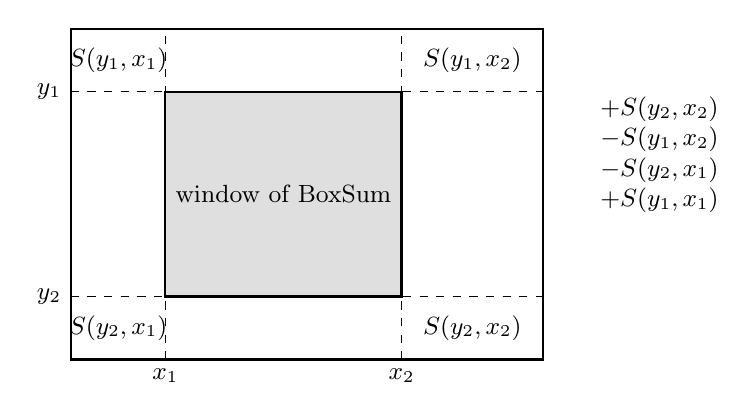
\begin{tikzpicture}[x=1cm,y=1cm]
\fill[gray!25] (1.2,0.8) rectangle (4.2,3.4);
\draw[thick] (0,0) rectangle (6,4.2);
\draw[thick] (1.2,0.8) rectangle (4.2,3.4);
\foreach \x/\l in {1.2/{$x_1$},4.2/{$x_2$}} {\draw[dashed] (\x,0) -- (\x,4.2); \node[font=\small,below] at (\x,0) {\l};}
\foreach \y/\l in {0.8/{$y_2$},3.4/{$y_1$}} {\draw[dashed] (0,\y) -- (6,\y); \node[font=\small,left] at (0,\y) {\l};}
\node[font=\small] at (2.7,2.1) {window of $\mathrm{BoxSum}$};
\node[font=\small] at (0.6,3.8) {$S(y_1,x_1)$};
\node[font=\small] at (5.1,3.8) {$S(y_1,x_2)$};
\node[font=\small] at (0.6,0.4) {$S(y_2,x_1)$};
\node[font=\small] at (5.1,0.4) {$S(y_2,x_2)$};
\node[font=\small,align=left,anchor=west] at (6.6,2.6) {$+S(y_2,x_2)$\\$-S(y_1,x_2)$\\$-S(y_2,x_1)$\\$+S(y_1,x_1)$};
\end{tikzpicture}
\caption{The four-corner rule of the summed-area table. Each table entry $S(y,x)$ is the sum of all pixels above and to the left of $(y,x)$ (measured with the vertical axis pointing down), so the shaded window sum follows from four entries (Equation~\ref{eq:seg-boxsum}).}
\label{fig:seg-boxsum}
\end{figure}

\paragraph{Dilation along one axis.}
The morphological dilation~\cite{haralick1987} that the block needs is always by a square, and a square dilation is separable into two one-dimensional dilations, each of which is again a window existence test and therefore again a cumulative sum.
With $c$ the cumulative sum of the boolean mask $m$ along the chosen axis, padded by $r+1$ before and $r$ after, the primitive is Equation~\ref{eq:seg-dilate},
\begin{equation}
\mathrm{AnyWithinRadius}(m,r)[i]=\bigl[\,c[i+2r+1]-c[i]>0\,\bigr]=\Bigl[\textstyle\bigvee_{k=-r}^{r} m[i+k]\Bigr],
\label{eq:seg-dilate}
\end{equation}
which is true wherever any set pixel lies within $r$ of position $i$ along that axis; applying Equation~\ref{eq:seg-dilate} once per axis dilates by a $(2r+1)\times(2r+1)$ square at a cost of two cumulative sums.
An \emph{erosion} of a mask is obtained as the dilation of its complement, complemented again, and a \emph{closing} as a dilation followed by an erosion; the block uses closings in three places and never needs any other structuring element.

\paragraph{Long straight runs along one axis.}
The second primitive answers, for every pixel, whether it lies on a run of at least $n$ consecutive set pixels along one axis.
With $c$ the cumulative sum of the mask along that axis, a run of length $n$ starts at index $i$ exactly when $c[i+n]-c[i]=n$; writing $\mathrm{hit}[i]$ for that indicator and $\mathrm{ch}$ for the cumulative sum of $\mathrm{hit}$, pixel $j$ is covered by some such run when Equation~\ref{eq:seg-runmask} holds,
\begin{equation}
\mathrm{LongRun}(m,n)[j]=\bigl[\,\mathrm{ch}[h_j+1]-\mathrm{ch}[l_j]>0\,\bigr],\qquad l_j=\max(0,j-n+1),\quad h_j=\min(j,L-n),
\label{eq:seg-runmask}
\end{equation}
where $L$ is the length of the axis and the window $[l_j,h_j]$ is the set of start positions of a run of length $n$ that could contain $j$; the mask is empty when $L<n$.
Equation~\ref{eq:seg-runmask} costs two cumulative sums and no loop, and it is the test on which the removal of printed rules in stage~4 rests.

\paragraph{The Gaussian kernel of the row profile.}
The only true Gaussian in the module is one-dimensional and short: the row-ink profile of stage~5 is smoothed by convolution with the 25-tap kernel of Equation~\ref{eq:seg-prof},
\begin{equation}
k[t]=\frac{\exp\bigl(-t^2/(2\sigma^2)\bigr)}{\sum_{u=-12}^{12}\exp\bigl(-u^2/(2\sigma^2)\bigr)},\qquad t=-12,\ldots,12,\qquad \sigma=4\ \text{rows},
\label{eq:seg-prof}
\end{equation}
so the kernel is truncated at exactly $3\sigma$, where the omitted tail carries about $0.3\,\%$ of the mass, and the normalisation makes the smoothed profile comparable with the raw one.
A standard deviation of four rows is about one tenth of a typical line pitch, which is enough to suppress the jitter caused by individual letters without merging two neighbouring line bodies into one peak.
Because the profile is a single vector of length $H$, a direct convolution costs $25H$ multiplications and no approximation is needed.

\paragraph{Equations retained from the earlier segmenter.}
An earlier segmenter approximated every blur as three successive box means of equal radius $r$~\cite{wells1986} \mustdo{confirm the page range of the Wells 1986 reference (IEEE TPAMI, vol.~8, no.~2) in the bibliography; it was left out rather than guessed.}, because the repeated convolution of a uniform kernel converges to a Gaussian shape by the central-limit argument.
A single box of full width $w=2r+1$ has the variance $(w^2-1)/12$, and three independent passes add their variances to
\begin{equation}
\sigma_{\mathrm{real}}^2=\frac{w^2-1}{4},\qquad w=2r+1,\qquad r=\max\Bigl(1,\;\mathrm{round}\Bigl(\tfrac12\sqrt{\tfrac{4\sigma^2}{3}+1}\Bigr)\Bigr),
\label{eq:seg-gauss}
\end{equation}
where $\sigma_{\mathrm{real}}$ is the realised standard deviation and $r$ the radius chosen for a requested nominal scale $\sigma$, so that $\sigma_{\mathrm{real}}\approx\sigma/\sqrt3\approx0.58\,\sigma$.
That earlier segmenter also converted a requested window width $B_w$ into an equivalent blur scale by the standard linear relation
\begin{equation}
\sigma_a=0.3\Bigl(\frac{B_w-1}{2}-1\Bigr)+0.8,
\label{eq:seg-sigmaa}
\end{equation}
in which $(B_w-1)/2$ is the window half-size.
\textbf{Neither Equation~\ref{eq:seg-gauss} nor Equation~\ref{eq:seg-sigmaa} is evaluated by the deployed module}, which uses a single box mean for the background (Equation~\ref{eq:seg-flat}) and the explicit kernel of Equation~\ref{eq:seg-prof} for the profile.
They are retained here, with their labels, because the segmentation timing figures reported in Section~\ref{sec:results} were measured on that earlier module and those figures include the cost of these constructions; a reader comparing the two must be able to see what was being timed.

\subsubsection{Stage 2: lighting normalisation and the ink mask}

The observed intensity of a photographed page is approximately paper reflectance times illumination, so the illumination is divided out rather than subtracted.
The background is estimated as a single box mean of the working grey image and the image is divided by it, Equation~\ref{eq:seg-flat},
\begin{equation}
\rho(p)=\frac{G(p)}{\max\bigl(\mathrm{BoxMean}_r(G)(p),\,1\bigr)},\qquad r=\max\Bigl(8,\;\min\bigl(40,\;\mathrm{round}(H/41)\bigr)\Bigr),
\label{eq:seg-flat}
\end{equation}
in which $G$ is the working grey image of stage~1, $H$ its height, $r$ the box radius, the clamp at 1 guards against division by a black background, and $\rho$ is the dimensionless \emph{ratio image} on which every threshold of the block acts.
On clean paper $\rho\approx1$ whatever the lighting; on ink $\rho$ is the local ink-to-paper reflectance ratio, which is a property of the pen and the paper and not of the lamp.
The radius of Equation~\ref{eq:seg-flat} is tied to the image height and clamped to $[8,40]$ so that it is always a few letter heights wide --- wide enough that a stroke does not darken its own background, narrow enough to follow a shadow edge --- and the clamp bounds the cost for a very large photograph.
Division rather than subtraction is used because the nuisance is multiplicative; subtracting a blurred copy would leave the ink contrast dependent on the local brightness, which is exactly what the next step must not depend on.
A limitation is that a large ink-heavy area, such as a dense diagram or a heavy correction block, is comparable in size with the blur window and therefore darkens its own background estimate, so its interior is partly flattened and may be lost.
Figure~\ref{fig:seg-illum} shows the effect on a real photograph.

\figplaceholder{5.2cm}{Four panels of the same photograph: (a) the colour photograph; (b) the working grey image $G$ after the $2{:}1$ box reduction; (c) the background estimate $\mathrm{BoxMean}_r(G)$ as a heat map, with the value of $r$ stated; (d) the ratio image $\rho$ of Equation~\ref{eq:seg-flat}. Source: call \texttt{SegmentLean.InkMask} on a personal page and save \texttt{BoxMean(gray,r)} and the returned \texttt{ratio} array; the module already returns $\rho$ as its second value, and the debug overlay it writes is $\rho$ scaled to 8 bits.}
\captionof{figure}{Lighting normalisation by division. The background estimate (c) follows the lighting gradient of the photograph, and dividing it out yields a ratio image (d) whose paper level is close to unity everywhere, on which a single global threshold is reliable.}
\label{fig:seg-illum}

\paragraph{A global threshold on the ratio image.}
Because the ratio image has already removed the slow shading, the ink decision can be a \emph{single global} threshold, which is chosen by Otsu's method~\cite{otsu1979}: the threshold that splits the histogram into a dark and a bright class so as to maximise the between-class variance, Equation~\ref{eq:seg-otsu},
\begin{equation}
t^*=\arg\max_t\;\omega_B(t)\,\omega_F(t)\,\bigl[\mu_B(t)-\mu_F(t)\bigr]^2,
\label{eq:seg-otsu}
\end{equation}
where $\omega_B(t)$ and $\omega_F(t)$ are the fractions of samples below and above $t$ and $\mu_B(t)$, $\mu_F(t)$ are the mean values of the two classes.
The product $\omega_B\omega_F$ is largest for a balanced split and the squared bracket largest for well-separated means, so Equation~\ref{eq:seg-otsu} places the cut where the two populations are most distinct.
The implementation evaluates the algebraically equivalent cumulative form of Equation~\ref{eq:seg-otsuimpl}, which needs one pass over the histogram and no inner loop,
\begin{equation}
\sigma_B^2(t)=\frac{\bigl[\mu_T\,\omega(t)-\mu(t)\bigr]^2}{\max\bigl(\omega(t)\,[1-\omega(t)],\;10^{-12}\bigr)},\qquad
\omega(t)=\sum_{i\le t}p_i,\quad \mu(t)=\sum_{i\le t} i\,p_i,\quad \mu_T=\mu(255),
\label{eq:seg-otsuimpl}
\end{equation}
in which $p_i$ is the normalised count of histogram bin $i$ and the clamp at $10^{-12}$ keeps the empty-class case finite.
The histogram has 256 bins spread uniformly over the ratio interval $[0,1.2]$, values outside being clipped into it, and the returned threshold is the centre of the winning bin, $t^*=(\arg\max+0.5)\times1.2/256$.
The upper limit 1.2 is deliberate: paper sits at $\rho\approx1$ and nothing above $1.2$ carries information about ink, so all of the resolution of the histogram is spent where the decision actually lies, and a specular highlight cannot drag the threshold.
The bin width is $1.2/256\approx0.0047$ in ratio units, which is far finer than the separation between ink and paper on any page tested.
A pixel is ink when $\rho<t^*$.

\paragraph{The solid-area veto.}
A global threshold on the ratio image still marks anything genuinely darker than its surroundings, which includes the interior of a binder shadow, a dark desk seen through a torn corner and the shaded gutter of a bound book.
Handwriting is thin: no pen stroke fills a $9\times9$ window completely.
The module therefore removes every region that does, Equation~\ref{eq:seg-solid},
\begin{equation}
\mathrm{solid}=\bigl[\mathrm{BoxMean}_4(\mathrm{ink})>0.999\bigr],\qquad
\mathrm{ink}\leftarrow\mathrm{ink}\wedge\neg\bigl[\mathrm{BoxMean}_3(\mathrm{solid})>0\bigr],
\label{eq:seg-solid}
\end{equation}
where $\mathrm{BoxMean}_4$ is the mean over a $9\times9$ window, so the first test is true only where all 81 pixels are ink, and the second test removes every pixel within a $7\times7$ window of such a centre, which strips the fringe of the blob as well as its interior.
The threshold 0.999 rather than 1 absorbs floating-point error in the integral image.
Equation~\ref{eq:seg-solid} is the one place where the block exploits a property of handwriting itself rather than of the photograph, and it is the reason the block tolerates a page photographed against a dark desk at all.
Its cost is that a very heavy marker stroke, or a filled-in letter counter in a large hand, is thinned at its centre; the halo recovery of stage~6 restores such pixels in the crop.

\paragraph{Why not a local threshold.}
A local adaptive threshold --- comparing each pixel with its own neighbourhood mean minus an offset --- is the usual answer for a photographed page, and it was what the earlier segmenter did, by Equation~\ref{eq:seg-adapt},
\begin{equation}
\mathrm{ink}(p)=\mathbb 1\bigl[\,I_{\mathrm c}(p)<M(p)-C\,\bigr]\wedge\mathrm{pageMask}(p),\qquad C=12,
\label{eq:seg-adapt}
\end{equation}
with $M$ a blurred copy of the corrected image, $\mathbb 1[\cdot]$ the indicator function and $C$ an offset in grey levels out of 255, together with a page-mask cut level derived from the median brightness $m_p$ inside the mask and $m_{bg}$ outside it,
\begin{equation}
c=\min\!\bigl(m_p-45,\;\max(m_p-85,\;\tfrac12(m_p+m_{bg}))\bigr).
\label{eq:seg-dark}
\end{equation}
\textbf{Neither Equation~\ref{eq:seg-adapt} nor Equation~\ref{eq:seg-dark} is evaluated by the deployed module}; both belonged to the earlier segmenter and are retained with their labels for the reason given above, namely that the timing figures of Section~\ref{sec:results} were measured on that module.
The deployed design replaces them with the single pair of Equations~\ref{eq:seg-flat} and~\ref{eq:seg-otsu} for three reasons that can be stated from the code alone.
First, the division has already removed the shading that the offset $C$ was there to survive, so the second local operation is redundant; second, a global threshold has no offset to tune, whereas $C$ in Equation~\ref{eq:seg-adapt} is a free parameter in grey levels that does not scale with pen contrast; and third, a local threshold necessarily marks \emph{something} in an empty region, because every region has a darkest pixel, which is precisely the behaviour that forced the earlier module's long chain of clean-up filters.
A threshold that also uses the local standard deviation~\cite{sauvola2000} would handle low-contrast regions better still, but it needs a second integral image of squared values and introduces two further constants; it was not adopted.
The cost of the global choice is honest and worth stating: a page whose illumination varies faster than the blur radius $r$ of Equation~\ref{eq:seg-flat} --- a hard shadow edge crossing the text, for instance --- is not corrected by the division, and a single global $t^*$ then either loses the dark side or floods the bright side.

\subsubsection{Stage 3: deskew by searching rotations}

If the text lines are tilted, a row-ink profile cannot resolve them, and the recogniser degrades as well.
The tilt is estimated by the classical projection-profile principle~\cite{postl1986}: when the lines are horizontal, the row-sum profile of the ink has sharp peaks at the line bodies and deep troughs between them, and any tilt smears both (Figure~\ref{fig:seg-skew}).
The module scores a candidate angle by the \emph{sum of squares} of the row profile, Equation~\ref{eq:seg-skew},
\begin{equation}
J(\theta)=\sum_y P_\theta(y)^2,\qquad P_\theta(y)=\sum_x R_\theta(y,x),\qquad \theta^*=\arg\max_\theta J(\theta),
\label{eq:seg-skew}
\end{equation}
where $R_\theta$ is the rotated ink mask and $P_\theta$ its row profile.
Equation~\ref{eq:seg-skew} is the variance criterion up to a constant: the total ink $\sum_y P_\theta(y)$ is very nearly invariant under rotation, so $\mathrm{Var}_y[P_\theta]=\frac1H\sum_yP_\theta^2-\bigl(\frac1H\sum_yP_\theta\bigr)^2$ differs from $J(\theta)/H$ by a term that is almost independent of $\theta$, and the two objectives have the same maximiser; the sum of squares is used because it needs no mean subtraction.
The search is a single exhaustive sweep of the 17 angles
\begin{equation*}
\theta\in\{-4.0^\circ,\,-3.5^\circ,\,\ldots,\,+3.5^\circ,\,+4.0^\circ\},
\end{equation*}
with no coarse-to-fine refinement, so the angular resolution is $0.5^\circ$ and the recoverable range is $\pm4^\circ$.
The mask that is rotated is the stage-2 ink mask reduced by a further factor two, that is one quarter of the photograph's linear size and one sixteenth of its area, so the whole search costs 17 rotations of a small mask plus 17 row sums.
Rotation about the image centre $(c_x,c_y)=((W-1)/2,(H-1)/2)$ uses inverse mapping,
\begin{equation}
\begin{pmatrix}x_s\\y_s\end{pmatrix}=\begin{pmatrix}\cos\theta&-\sin\theta\\ \sin\theta&\cos\theta\end{pmatrix}\begin{pmatrix}x-c_x\\y-c_y\end{pmatrix}+\begin{pmatrix}c_x\\c_y\end{pmatrix},
\label{eq:seg-rot}
\end{equation}
in which $(x,y)$ is an output pixel and $(x_s,y_s)$ the source position that is sampled.
Inverse mapping as in Equation~\ref{eq:seg-rot} is used, rather than mapping the source forward, because every output pixel then receives exactly one value and no holes can appear.
The candidate masks are rotated with nearest-neighbour sampling and a fill value of 0, so that the area outside the page contributes no ink and cannot flatten the profile; the page itself is then rotated once, bilinearly, with a fill value of 255, so that the corners brought in are white paper and not black.
Both the full-resolution page and the working image are rotated by the chosen $\theta^*$, and the ink mask and the ratio image are then \emph{recomputed} on the rotated working image, because the box mean of Equation~\ref{eq:seg-flat} is not rotation-equivariant.

\begin{figure}[h]
\centering
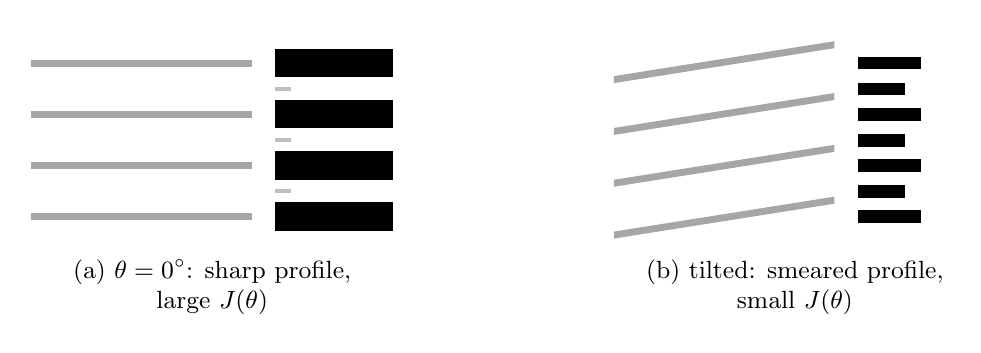
\begin{tikzpicture}[x=1cm,y=1cm]
% left: aligned lines
\begin{scope}
\foreach \k in {0,1,2,3} {\draw[line width=2.5pt,gray!70] (0,\k*0.65) -- (2.8,\k*0.65);}
\foreach \k in {0,1,2,3} {\fill[black] (3.1,\k*0.65-0.18) rectangle (3.1+1.5,\k*0.65+0.18);}
\foreach \k in {0,1,2} {\fill[black!25] (3.1,\k*0.65+0.3) rectangle (3.1+0.2,\k*0.65+0.35);}
\node[font=\small,align=center] at (2.3,-0.9) {(a) $\theta=0^\circ$: sharp profile,\\ large $J(\theta)$};
\end{scope}
% right: tilted lines
\begin{scope}[xshift=7.4cm]
\begin{scope}
\clip (0,-0.4) rectangle (2.8,2.4);
\foreach \k in {0,1,2,3} {\draw[line width=2.5pt,gray!70,rotate around={9:(1.4,1.0)}] (-0.4,\k*0.65) -- (3.2,\k*0.65);}
\end{scope}
\foreach \k in {0,1,2,3} {\fill[black] (3.1,\k*0.65-0.08) rectangle (3.1+0.8,\k*0.65+0.08);}
\foreach \k in {0,1,2} {\fill[black] (3.1,\k*0.65+0.24) rectangle (3.1+0.6,\k*0.65+0.40);}
\node[font=\small,align=center] at (2.3,-0.9) {(b) tilted: smeared profile,\\ small $J(\theta)$};
\end{scope}
\end{tikzpicture}
\caption{Principle of the projection objective of Equation~\ref{eq:seg-skew}. The bars on the right of each panel represent the row-sum profile of the ink. Aligned lines (a) give strong peaks and empty gaps and therefore a large sum of squares, whereas a tilt (b) fills the gaps and lowers it. The same profile is used again in stage~5 to find the line centres.}
\label{fig:seg-skew}
\end{figure}

\paragraph{Skew limitations and alternatives.}
The objective of Equation~\ref{eq:seg-skew} was preferred to a Hough transform~\cite{duda1972} of ink edges, because the latter is dominated by ruled lines and diagram strokes, whereas the projection objective is aligned with what the next stages need, namely a resolvable row profile; it is also the same quantity that stage~5 then reuses, so the page is scored by the criterion it is afterwards judged on.
Four limitations follow directly from the code and must be stated.
The range is only $\pm4^\circ$, so a page placed more crookedly than that is not straightened at all and the block will fail on it; the resolution is $0.5^\circ$, so a residual tilt of up to $0.25^\circ$ always remains, which over a 2000-pixel line is about 9 pixels of drift; a single global angle is estimated, so page curl and perspective keystone are not corrected; and the rotation is applied unconditionally, with no dead band around zero, so an already-straight page is resampled once for nothing, which costs a little sharpness.
The earlier segmenter searched $\pm8^\circ$ with a $0.1^\circ$ second pass and corrected the drift of each individual line afterwards by the least-squares fit of Equation~\ref{eq:seg-lsq} below; the deployed module does neither, and the residual per-line drift is simply carried into the crop.
One piece of design history belongs here: in the earlier module a sign mismatch between the rotation routine and the angle scorer was found to have \emph{doubled} the skew of every tilted page.
The deployed module is immune to that class of error by construction rather than by care, because the candidate masks are rotated by the same library call, with the same sign convention, that is afterwards applied to the page.
Figure~\ref{fig:seg-skewmeas} is reserved for a measured example of the objective.

\figplaceholder{4.4cm}{Skew search on a deliberately tilted photograph: left, a plot of $J(\theta)$ of Equation~\ref{eq:seg-skew} over the 17 candidate angles with the chosen $\theta^*$ marked; right, the page before and after rotation with the angle printed. Source: the loop inside \texttt{SegmentLines} that evaluates \texttt{max(np.arange(-4,4.01,0.5), key=...)}; store the score of every candidate instead of only the maximiser. The chosen angle is also returned in the statistics dictionary as the field \texttt{angle}.}
\captionof{figure}{Measured skew-search objective $J(\theta)$ (placeholder).}
\label{fig:seg-skewmeas}

\subsubsection{Stage 4: paper region, long straight runs and page-boundary artefacts}

A first estimate of the line pitch $P$ is now computed from the ink mask (the procedure is that of stage~5, applied here to the uncleaned mask) because every threshold of this stage is expressed in units of $P$.
Three removals then follow in order: everything outside the sheet, every long straight run, and every remaining piece of ink whose shape and position identify it as a page-boundary artefact rather than writing.

\paragraph{The paper region.}
The desk, a hand or a facing page must not contribute ink, so a boolean \emph{paper region} is estimated, and the construction exploits the fact that handwriting disappears under a sufficiently coarse average while the sheet does not.
The working grey image is reduced by a further factor $s=4$ by block averaging, blurred with a box mean of radius $\max(1,\lfloor0.15P/s\rfloor)$, and a cell is called dark when its value is below $0.45$ times the median of the reduced image.
If fewer than $0.2\,\%$ of the cells are dark there is no surround to cut away and the whole frame is accepted as paper, which is the correct answer for a photograph that is filled by the sheet.
Otherwise the bright set is labelled, its largest connected component is taken as the sheet, expanded back by a factor $s$ in each direction, and any rows or columns lost to the truncation of the reduction are counted as paper; the region is finally eroded by $\lfloor0.4P\rfloor$ on each axis with two applications of Equation~\ref{eq:seg-dilate}, so that the darkened rim of the sheet itself is not binarised as ink.
The factor $0.45$ on the median is the only brightness constant here, and it is a ratio rather than a level, so it survives a change of exposure; the erosion depth is in units of $P$, so it is about two fifths of a line spacing on any page.
The fraction of the frame that was accepted is reported as \texttt{paperCoverage} and the amount of ink discarded by this step as \texttt{inkOutsidePaper}, which makes the step auditable from the returned statistics alone.
The method fails when the desk is almost as bright as the paper, in which case the largest bright component swallows the desk; the fallback, as above, is the whole frame.
Figure~\ref{fig:seg-mask} is reserved for an example.

\figplaceholder{4.6cm}{Paper-region construction as a $2\times2$ panel: the $4\times4$-reduced blurred image, the dark set at $0.45\times$ its median, the largest bright component expanded back, and the final region after the $\lfloor0.4P\rfloor$ erosion overlaid on the photograph. Source: \texttt{SegmentLean.PaperRegionMask(g,P)}; the debug overlay that \texttt{SegmentLines} already writes (\texttt{\_cuts\_overlay.jpg}) tints everything outside this region red, so panel four can be cropped from it.}
\captionof{figure}{Construction of the paper region (placeholder).}
\label{fig:seg-mask}

\paragraph{Long straight runs: printed rules, underlines and the binder edge.}
Ruled paper, an underline and the straight shadow at the spine of a bound book all join words and lines into one giant piece of ink, and all three share one property that handwriting does not have: they are straight for longer than a line spacing.
The test is therefore the long-run primitive of Equation~\ref{eq:seg-runmask}, applied once per axis and bracketed by a dilation and a re-intersection so that a run broken by a slight tilt or by a crossing stroke still counts, Equation~\ref{eq:seg-cand},
\begin{equation}
\begin{aligned}
\mathrm{flat}&=\mathcal D_{1}^{y}\Bigl(\mathrm{LongRun}^{x}\bigl(\mathcal D_{1}^{y}(\mathrm{ink}),\;\lfloor1.25P\rfloor\bigr)\Bigr)\wedge\mathrm{ink},\\
\mathrm{upright}&=\mathcal D_{3}^{x}\Bigl(\mathrm{LongRun}^{y}\bigl(\mathcal D_{3}^{x}(\mathrm{ink}),\;\lfloor1.4P\rfloor\bigr)\Bigr)\wedge\mathrm{ink},
\end{aligned}
\label{eq:seg-cand}
\end{equation}
where $\mathcal D_r^{y}$ and $\mathcal D_r^{x}$ are the one-axis dilations of Equation~\ref{eq:seg-dilate} by radius $r$ along the row and the column axis, and the removed set is $\mathrm{flat}\vee\mathrm{upright}$.
The inner dilation is what makes Equation~\ref{eq:seg-cand} tolerant: dilating by one row before the horizontal run test lets a rule that drifts by a pixel over its length still read as a single run, and the generous radius of three columns for the vertical test absorbs the wobble of a photographed page edge.
The outer dilation grows the detected run back to the thickness it was given, and the final intersection with the ink mask guarantees that only pixels that were ink are removed.
The length thresholds are the essential point: a horizontal run must exceed $1.25P$ and a vertical run $1.4P$, both longer than any letter can be, since $P$ is the spacing between lines and a letter occupies well under half of it.
A long word written without a pen lift is not at risk, because a word is not straight to within one dilated row over $1.25P$.
The number of pixels removed is reported as \texttt{removedStraightPixels}.
The weakness of Equation~\ref{eq:seg-cand} is equally clear: a rule that is both faint and broken into fragments shorter than $1.25P$ survives it, and a deliberate long straight pen stroke --- a division bar in an equation, a strike-through --- is removed as though it were printed.
The earlier segmenter attacked the same problem by chaining short rule fragments across gaps, admitting a vertical offset of
\begin{equation}
|c_{y,b}-c_{y,a}|\le\Delta_{\max}=2\kappa+0.08\max(0,g)+0.04\,(w_a+w_b)
\label{eq:seg-slope}
\end{equation}
between two fragments separated by a gap $g$, where $c_y$ is a centroid row, $w$ a width and $\kappa$ a thickness cut.
\textbf{Equation~\ref{eq:seg-slope} is not evaluated by the deployed module}; it is retained with its label for the reason given above.
Dropping fragment chaining is a deliberate simplification --- it removed a group of constants ($\kappa$, the two slope allowances, the page-crossing span tests) at the cost of the broken-rule case just described.

\paragraph{Page-boundary artefact pieces.}
What survives the two steps above is still not all writing: edge slivers, corner shadows and fold creases remain, and they cannot be identified pixel by pixel because each is individually faint and locally indistinguishable from a stroke.
They are identified as whole \emph{pieces}.
The ink mask is closed by a square of radius $r_c=\max(1,\lfloor0.1P\rfloor)$ --- a dilation followed by an erosion, both by Equation~\ref{eq:seg-dilate} --- so that the pen lifts inside a word are bridged and a word becomes one piece, and the closed mask is labelled by the algorithm of the next subsubsection.
Every statistic is then accumulated over the \emph{original} ink pixels of each piece, so the closing decides what belongs together but never contributes area.
For a piece with area $A$, bounding box $[x_{\min},x_{\max}]\times[y_{\min},y_{\max}]$, height $h=y_{\max}-y_{\min}+1$ and width $w=x_{\max}-x_{\min}+1$, the module forms the predicates of Table~\ref{tab:seg-artifact} with $e=\max(3,\lfloor0.5P\rfloor)$ as the distance from the frame that counts as touching it.
Two of them need a measure of faintness, for which the mean ratio over the piece is compared with the page's own ink threshold, Equation~\ref{eq:seg-dark2},
\begin{equation}
\bar\rho_c=\frac{1}{A_c}\sum_{p\in c}\rho(p),\qquad \mathrm{faint}(c)=\bigl[\,\bar\rho_c>0.85\,t^*\,\bigr],
\label{eq:seg-dark2}
\end{equation}
where $t^*$ is the Otsu threshold of Equation~\ref{eq:seg-otsu} on the same ratio image.
A piece is faint when its average ink is only just past the threshold that admitted it; a real pen stroke is much darker than $0.85\,t^*$, whereas a crease or a printed rule sits barely below $t^*$ by construction, because that is how it got in.
Expressing faintness relative to $t^*$ rather than as a fixed level is what lets the same constant serve a pencil page and a fibre-tip page.
A further reference quantity is the \emph{text margin} $x_L$, the fifth percentile of the left edges of all letter-like pieces, a piece being letter-like when $A\ge0.065P^2$ and $h\le2.2P$; any piece lying entirely more than $1.2P$ to the left of $x_L$ is outside the text block and is discarded.
The number of pieces discarded is reported as \texttt{artifactPieces}.

\begin{table}[h]
\centering
\fontsize{9.5}{11.5}\selectfont
\begin{tabularx}{\linewidth}{|p{3.3cm}|X|}
\hline
\textbf{Discard condition} & \textbf{What it is meant to catch} \\
\hline
$x_{\min}\le e$ & Any piece touching the left frame edge: the sliver of the facing page or of the desk that the paper erosion left behind. \\
\hline
$x_{\max}\ge W-1-e$ and $w\le0.5P$ & A narrow sliver at the right frame edge; a real line reaching the right edge is wider than $0.5P$. \\
\hline
$y_{\min}\le e$ or $y_{\max}\ge H-1-e$, with $h\le0.5P$ and $w\le0.5P$ & A small fleck at the top or bottom frame edge. \\
\hline
$h>2.2P$ and $w\le0.5P$ & A tall thin streak spanning more than two line spacings: a binder edge or a fold. \\
\hline
$w\le0.12P$ and $h\ge1.2P$ & A vertical bar thinner than any letter and taller than any letter. \\
\hline
$\mathrm{faint}$, $w\le0.2P$ and $h\ge0.6P$ & A faint vertical bar: a printed margin rule or a crease. \\
\hline
$(y_{\min}\le e$ or $y_{\max}\ge H-1-e)$, $h\le1.2P$, $A/(hw)<0.15$, $\mathrm{faint}$ and $w>P$ & An edge shadow or fold: wide, faint, at an edge, and so sparse inside its own box that it cannot be writing. \\
\hline
$x_{\max}<x_L-1.2P$ & A piece entirely left of the text margin: a hole punch, a staple shadow, a page number in the gutter. \\
\hline
\end{tabularx}
\caption{The eight discard predicates applied to each closed piece of ink in stage~4, with $e=\max(3,\lfloor0.5P\rfloor)$, $x_L$ the fifth percentile of the left edges of letter-like pieces, and $\mathrm{faint}$ as defined by Equation~\ref{eq:seg-dark2}. The background label is exempt from all of them.}
\label{tab:seg-artifact}
\end{table}

The first row of Table~\ref{tab:seg-artifact} is the most aggressive rule in the module and its cost must be stated plainly: \emph{any} piece whose leftmost ink lies within $\max(3,\lfloor0.5P\rfloor)$ of the left edge of the frame is discarded regardless of its size or darkness, so a page photographed so tightly that the writing itself reaches the left edge loses the first letters of those lines.
The rule is safe for the intended use, in which the sheet is photographed with a visible margin, and it is the single rule that removes the facing page of an open book, which no shape test alone could do.
A second limitation of this stage is that it owns no model of what text \emph{is}: a diagram, a table or a stamp that is dark, compact and inside the text margin passes every predicate and is handed on to stage~5 as though it were writing.

\subsubsection{Stage 5a: connected components}

A \emph{connected component} is a maximal set of mask pixels that touch each other, diagonal neighbours included (8-connectivity).
Components are found with a run-length two-pass algorithm with union-find, a design that follows the classical sequential labelling idea~\cite{rosenfeld1966} but works on runs instead of single pixels.
Each image row is first encoded as maximal runs $[s,e)$ of set pixels, obtained from the differences of the row against a zero-padded copy of itself, so that a $+1$ marks a run start and a $-1$ a run end; no per-pixel loop is involved in finding the runs.
For every pair of adjacent rows the runs are swept with two pointers, and run $i$ of the upper row and run $j$ of the lower row are merged when they touch; for 8-connectivity the condition (Equation~\ref{eq:seg-adj}) is
\begin{equation}
s_i<e_j+1\ \ \wedge\ \ s_j<e_i+1,
\label{eq:seg-adj}
\end{equation}
and for 4-connectivity the $+1$ terms are dropped, where $s$ and $e$ are the start and end (exclusive) columns of the runs.
The pointer whose run ends first is advanced, so each row pair is swept once.
The merging uses a union-find structure with path halving~\cite{tarjan1984}, one of the one-pass compaction rules whose almost-linear amortised cost follows from Tarjan's analysis of path compression~\cite{tarjan1975}; the union itself always attaches the larger root index to the smaller, which keeps the labels of the first-seen components stable.
Roots are finally mapped to compact labels $1\ldots n$ by a sort-and-invert step, label 0 being the background, and the labels are painted back run by run.
The cost is linear in the number of runs times an almost constant factor, which is far cheaper than a pixel-wise method for thin handwriting strokes, where a run is typically several pixels long.
The routine is called on the closed mask (stage~4), on the raw mask (the dot rules of stage~6), inside the paper-region estimate, inside the pitch fallback and once per band when the fragment rule runs; it is the most frequently invoked primitive in the module.

\subsubsection{Stage 5b: line pitch and line centres from the row-ink profile}

This is the stage at which the deployed design departs most sharply from the earlier one, and the departure is in favour of the \emph{simpler} method, so the justification matters.

\paragraph{The profile.}
The row-ink profile is the number of mask pixels in each row, taken over the horizontal interval from $0.05W$ to $0.97W$ so that the extreme left and right of the frame cannot contribute, and smoothed with the Gaussian kernel of Equation~\ref{eq:seg-prof}:
\begin{equation}
\mathrm{prof}(y)=\sum_{x=\lfloor0.05W\rfloor}^{\lfloor0.97W\rfloor-1}\mathrm{ink}(y,x),\qquad \mathrm{sm}=\mathrm{prof}*k .
\label{eq:seg-pitch}
\end{equation}
A \emph{peak} of the smoothed profile is an interior row $y$ with
\begin{equation}
\mathrm{sm}(y)\ge\mathrm{sm}(y-1),\qquad \mathrm{sm}(y)>\mathrm{sm}(y+1),\qquad \mathrm{sm}(y)>0.06\max_u\mathrm{sm}(u),
\label{eq:seg-centres}
\end{equation}
the asymmetric pair of comparisons in Equation~\ref{eq:seg-centres} selecting the \emph{last} row of a flat plateau exactly once, so that a broad line body yields one peak and not a cluster of them, and the relative floor of $0.06$ of the maximum rejecting the ripple that stray marks leave between the lines.
The line pitch is then the median of the gaps between consecutive peaks,
\begin{equation*}
P=\mathrm{median}\bigl\{y_{i+1}-y_i\bigr\},
\end{equation*}
whenever at least two peaks exist, which is the case for every multi-line page.
Taking the median of the \emph{observed} gaps, rather than fitting one periodicity to the page, is what lets the pitch be right on a page whose paragraph spacing is irregular, and the module's own comment records that this choice was checked against sixteen real pages.

\paragraph{Three fallbacks.}
When fewer than two peaks are resolved, the pitch is estimated from the autocorrelation of the mean-removed smoothed profile $a=\mathrm{sm}-\overline{\mathrm{sm}}$: the non-negative-lag part of $a\star a$ is examined over lags $15$ to $\min(200,\lfloor L_{ac}/3\rfloor)$, and the first local maximum reaching $0.7$ of the segment maximum gives $P$.
The lower lag bound of 15 rows excludes the central spike and the upper bound of one third of the correlation length keeps the estimate inside the region where the correlation is still supported by enough overlap.
This branch is a fallback and not the primary method precisely because it can lock onto a \emph{multiple} of the true spacing on a page with uneven paragraph gaps, which the direct peak gap cannot.
If the autocorrelation gives nothing either --- a page with a single line of writing, where there is no spacing to measure --- the scale is taken from the letters themselves, by the median height of the plausible components, Equation~\ref{eq:seg-ht},
\begin{equation}
P=\max\bigl(15,\ \mathrm{round}\bigl(2.2\,\mathrm{median}\{h_c\}\bigr)\bigr),\qquad c:\ A_c\ge8\ \wedge\ 3\le h_c\le H,
\label{eq:seg-ht}
\end{equation}
where $h_c$ and $A_c$ are the height and the area of component $c$; the area floor of 8 pixels and the height floor of 3 rows exclude speckle, and the factor $2.2$ is the empirical ratio of line pitch to letter height for the hands in this project.
Equation~\ref{eq:seg-ht} is the only place where a glyph height still sets the scale, and it is a last resort rather than the primary unit, which is the substantive difference from the earlier segmenter: there, a median glyph height $\wht$ obtained by a median-of-medians over the components was the scale unit of the \emph{whole} block, so a page with one unusually large heading rescaled every threshold on it.
If no component qualifies at all, $P=48$ rows, an arbitrary but harmless default on a page that has no usable ink.

\paragraph{The line centres.}
The pitch and the profile are recomputed once on the \emph{cleaned} mask, after stage~4, because removing a ruled line or a shadow changes both.
The peaks of Equation~\ref{eq:seg-centres} are then turned into line centres by a greedy non-maximum suppression in units of the pitch: the peaks are visited in order of decreasing profile value and a peak is accepted as a centre only if it is at least $0.6P$ from every centre already accepted; the accepted set is finally sorted by row.
Visiting the strongest peak first means that where two peaks fall within $0.6P$ of each other --- the body of a line and the band of its own ascenders, for instance --- the one carrying more ink wins, which is the line body.
The separation floor of $0.6P$ is somewhat more than half a pitch, so two genuine lines can never be merged while a doubled peak inside one line can never be split.
Figure~\ref{fig:seg-chain} shows the profile, the centres and the seams of stage~6 together.

\paragraph{Why a row profile was chosen, and what it cannot do.}
The earlier segmenter rejected a row projection and grouped the components instead, by chaining each component to a successor on its right under the cost
\begin{equation}
\mathrm{cost}(a,b)=\max(0,\mathrm{gap})+3\,\Delta y,
\label{eq:seg-cost}
\end{equation}
with $\mathrm{gap}$ the horizontal distance between bounding boxes and $\Delta y$ the offset of the centroid rows, and by giving each resulting chain an area-weighted five-point moving-average baseline
\begin{equation}
\tilde y_i=\frac{\sum_{k=i-2}^{i+2}A_k\,y_k}{\sum_{k=i-2}^{i+2}A_k}.
\label{eq:seg-curve}
\end{equation}
\textbf{Neither Equation~\ref{eq:seg-cost} nor Equation~\ref{eq:seg-curve} is evaluated by the deployed module}, which uses the row profile of Equations~\ref{eq:seg-pitch} and~\ref{eq:seg-centres} instead; both are retained with their labels for the reason given above.
The reversal was deliberate and is justified as follows.
Chaining needs a correct component set before it can start, so every error of the clean-up stages propagates into the line structure, and it needs a chain-merging policy on top, which in the earlier module came to three passes with ten further constants and a quadratic worst case; the profile needs no component set at all, costs one pass over the mask, and produces the scale unit $P$ and the line centres from the same computation, so the page's own spacing calibrates the thresholds that are then applied to it.
Against that, three weaknesses of the profile are real and are accepted.
It assumes a single dominant horizontal orientation, so it is only as good as the $\pm4^\circ$ deskew that precedes it and it cannot represent a baseline that curves within one line; it assumes one column, so a two-column page or a diagram beside the text contributes peaks that belong to no single line and will be read as spurious lines or will corrupt $P$; and it has no notion of what text is, so it offers nothing like the text-versus-diagram separation the earlier module attempted.
A fourth weakness is a threshold rather than a principle: the floor of $0.06\max\mathrm{sm}$ in Equation~\ref{eq:seg-centres} will silently discard a line so faint or so short that its peak falls below six per cent of the strongest line's peak.
\mustdo{measure how often the $0.06\max\mathrm{sm}$ floor of Equation~\ref{eq:seg-centres} discards a real line. The quantity to report is the number of lines missed over the test pages, against the hand-counted line total; nothing in the project files records it.}
Finally, and most seriously, the module has no guard for the case in which \emph{no} peak clears that floor: an empty or near-empty page yields an empty set of centres, and the construction of the first cut then indexes the first centre of an empty list, which raises an exception rather than returning zero lines.
The same applies to the text margin $x_L$ of stage~4 when no piece is letter-like.
Both are blank-page failure modes, not misreadings, and the server should reject such an image before calling the block.

\subsubsection{Stage 6a: least-ink seams by dynamic programming}

The line centres say where the lines are; the boundaries between them are found as paths that cross as little ink as possible.
A straight horizontal cut halfway between two centres would sever every descender of the upper line and every ascender of the lower one, so the boundary is allowed to bend.
Between two consecutive centres $c_0<c_1$ the module builds the cost field of Equation~\ref{eq:seg-cost2} over the rows of that gap,
\begin{equation}
C(y,x)=4.0\,\tilde m(y,x)+0.012\left(\frac{y-\mu}{\max(1,(c_1-c_0)/2)}\right)^{\!2},\qquad \mu=c_0+\tfrac12(c_1-c_0),
\label{eq:seg-cost2}
\end{equation}
in which $\tilde m$ is the closed ink mask as a 0/1 field, $\mu$ the midline of the gap and the denominator a normalisation to the half-width of the gap, so that the second term is $0.012$ at the two centres and zero at the midline.
The first term of Equation~\ref{eq:seg-cost2} is the one that matters: with a weight of $4.0$ against a maximum of $0.012$ for the midline term, crossing a single ink pixel is more than three hundred times as expensive as sitting one half-gap away from the midline, so the path will take almost any detour to avoid ink and the midline term only breaks ties over the large empty areas between words.
Without that weak pull the path would wander arbitrarily far through the empty space and could leave the gap entirely; with it, the path traces real ink where there is ink and relaxes to a straight line where there is none.

The cheapest such path is found by dynamic programming over columns, Equation~\ref{eq:seg-seam},
\begin{equation}
A(y,x)=C(y,x)+\min_{|d|\le s}\bigl[\,A(y+d,\,x-1)+0.02\,|d|\,\bigr],\qquad s=7,
\label{eq:seg-seam}
\end{equation}
with $A(y,0)=C(y,0)$, where $d$ is the row displacement taken between column $x-1$ and column $x$ and the term $0.02|d|$ is a small penalty for not going straight ahead.
The chosen $d$ is stored for every cell, the path end is the row minimising $A(\cdot,W-1)$, and the path is recovered by following the stored displacements back to the first column.
Equation~\ref{eq:seg-seam} is exact: because the cost of a path is a sum over columns and the recursion considers every admissible predecessor, the value $A(y,x)$ is the true minimum cost of any admissible path from column 0 to cell $(y,x)$, and no search heuristic is involved.
The step limit $s=7$ rows per column is what lets the boundary react to a tall narrow descender rather than cutting through it, and the penalty $0.02$ per row of displacement --- weak against the ink weight $4.0$ but not negligible against the midline term --- keeps the path from zig-zagging where nothing forces it to move.
The mask used in Equation~\ref{eq:seg-cost2} is first closed by a square of radius $\max(2,\lfloor0.07P\rfloor)$; the module's own comment gives the reason, which is that a plain dilation would inflate every stroke into a blob and the cut would then trace the blob, whereas a closing fills only the thin gap beside a letter stem through which a path could otherwise thread, leaving the outer shape of the stroke close to the truth.
The outermost two boundaries are not computed but fixed: a constant row at $\max(0,c_{\mathrm{first}}-\lfloor0.75P\rfloor)$ above the first centre and at $\min(H-1,c_{\mathrm{last}}+\lfloor0.75P\rfloor)$ below the last, three quarters of a pitch being enough to contain the ascenders of the first line and the descenders of the last.
With $L$ centres there are therefore $L+1$ boundaries and $L$ bands.
Evaluating Equation~\ref{eq:seg-seam} costs $(2s+1)=15$ candidate comparisons per cell, and the cells of all gaps together are at most the rows of the page times its columns, so the whole seam computation is $O(15\,HW)$ in the worst case and in practice proportional to the ink-bearing height of the page.

\begin{figure}[h]
\centering
\begin{tikzpicture}[x=1cm,y=1cm]
% page area with three rows of text
\draw[thick] (0,0) rectangle (7.6,4.6);
% line 1 bodies
\foreach \x in {0.4,1.3,2.1,3.2,4.2,5.4,6.4} {\fill[gray!45] (\x,3.45) rectangle (\x+0.55,3.95);}
\fill[gray!45] (2.35,3.0) rectangle (2.5,3.5); % descender of line 1
% line 2 bodies
\foreach \x in {0.4,1.2,2.0,3.1,4.0,5.2,6.2} {\fill[gray!45] (\x,2.1) rectangle (\x+0.55,2.6);}
\fill[gray!45] (4.55,2.55) rectangle (4.7,3.15); % ascender of line 2
% line 3 bodies
\foreach \x in {0.4,1.4,2.4,3.4,4.5} {\fill[gray!45] (\x,0.75) rectangle (\x+0.55,1.25);}
% centres
\foreach \y/\l in {3.7/{$c_1$},2.35/{$c_2$},1.0/{$c_3$}} {
  \draw[dashed,gray] (0,\y) -- (7.6,\y);
  \node[font=\scriptsize,anchor=east] at (-0.08,\y) {\l};}
% seams
\draw[thick,red] plot[smooth,tension=0.7] coordinates {(0,3.05) (1.0,3.05) (2.0,3.05) (2.25,2.88) (2.6,2.88) (2.85,3.05) (4.0,3.05) (4.45,3.22) (4.8,3.22) (5.1,3.05) (6.4,3.05) (7.6,3.05)};
\draw[thick,blue] plot[smooth,tension=0.7] coordinates {(0,1.68) (1.5,1.68) (3.0,1.68) (4.5,1.68) (6.0,1.68) (7.6,1.68)};
% profile on the right
\begin{scope}[xshift=8.1cm]
\draw[->] (0,0) -- (0,4.6);
\draw[->] (0,0) -- (2.5,0) node[below,font=\scriptsize,anchor=north west] {$\mathrm{sm}(y)$};
\draw[thick] plot[smooth] coordinates {(0.05,0.2) (0.1,0.6) (0.9,1.0) (2.1,1.25) (0.9,1.45) (0.12,1.68) (0.08,1.9) (1.0,2.15) (2.3,2.35) (1.0,2.6) (0.1,2.85) (0.3,3.05) (0.12,3.25) (1.1,3.5) (2.25,3.7) (1.1,3.9) (0.1,4.15) (0.05,4.4)};
\draw[dashed,gray] (0,3.7) -- (2.4,3.7);
\draw[dashed,gray] (0,2.35) -- (2.4,2.35);
\draw[dashed,gray] (0,1.25) -- (2.4,1.25);
\fill[black] (2.25,3.7) circle (1.6pt);
\fill[black] (2.3,2.35) circle (1.6pt);
\fill[black] (2.1,1.25) circle (1.6pt);
\node[font=\scriptsize,anchor=west] at (2.4,3.7) {peak};
\draw[<->] (2.75,2.35) -- (2.75,3.7);
\node[font=\scriptsize,anchor=west] at (2.8,3.0) {$P$};
\end{scope}
\node[w2lab,anchor=south west] at (0.1,4.15) {seams bend around a descender and an ascender};
\end{tikzpicture}
\caption{Line pitch, centres and seams. The smoothed row-ink profile on the right has one peak per line body; the median gap between peaks is the pitch $P$ and the suppressed peaks are the line centres $c_i$ (Equations~\ref{eq:seg-pitch} and~\ref{eq:seg-centres}). Each boundary between two centres is the least-cost path of Equation~\ref{eq:seg-seam}, which detours around the descender of the line above and the ascender of the line below (red) and relaxes to a straight line where the gap is empty (blue).}
\label{fig:seg-chain}
\end{figure}

\subsubsection{Stage 6b: pixel ownership}

The seams divide the page into $L$ bands, and the default rule is the simplest possible one: an ink pixel belongs to the band it lies in.
Writing is not that tidy, however --- a descender crosses a seam, an $i$ dot sits a long way above its own line's body, a comma dangles below it --- so five correction rules act on top of the default, all of them stated in units of $P$ and $P^2$ and all of them conservative in the sense that a piece is only ever moved to an \emph{adjacent} band or dropped.
The band index of a pixel is obtained without any search, as the number of interior boundaries above it,
\begin{equation}
\mathrm{band}(y,x)=\sum_{n=1}^{L-1}\bigl[\,y\ge\mathrm{cut}_n(x)\,\bigr],
\label{eq:seg-band}
\end{equation}
Equation~\ref{eq:seg-band} is a single accumulation over the boundaries and gives $0$ for the top band and $L-1$ for the bottom one; pixels above the first boundary or below the last are outside every band and are never emitted.
For each piece $c$ of the closed labelling and each band $n$, the module counts the ink $N_{c,n}$ of that piece inside that band, and the ownership decision rests on the share
\begin{equation}
\mathrm{share}_{c,n}=\frac{N_{c,n}}{\sum_{m}N_{c,m}},\qquad
\mathrm{major}(c)=\begin{cases}\min\{n:\mathrm{share}_{c,n}\ge0.15\} & \text{if any share reaches }0.15,\\[2pt] \arg\max_n N_{c,n} & \text{otherwise.}\end{cases}
\label{eq:seg-share}
\end{equation}
A share of $0.15$ is the threshold at which a piece is held to have a genuine presence in a band, and the choice of the \emph{topmost} such band in Equation~\ref{eq:seg-share} rather than the largest is deliberate: when a piece really does span two lines, the crop that goes wrong if it loses the piece is the upper one, whose descender it is.
Figure~\ref{fig:seg-ramp} collects the size thresholds that the rules below use.

\begin{figure}[h]
\centering
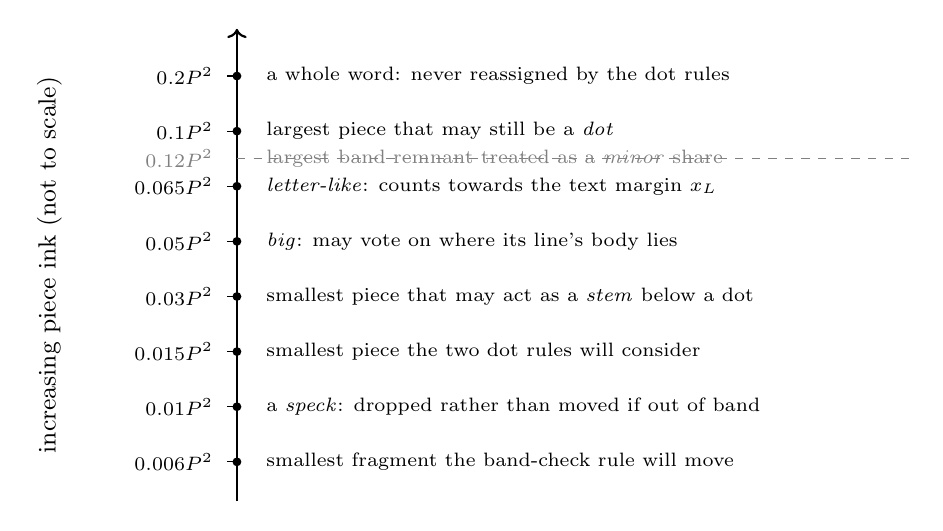
\begin{tikzpicture}[x=1cm,y=1cm]
\tikzset{sz/.style={font=\scriptsize,anchor=west}}
\draw[->,thick] (0,0) -- (0,6.0);
\node[font=\small,rotate=90,anchor=south] at (-2.1,3.0) {increasing piece ink (not to scale)};
\foreach \y/\v/\t in {
  0.5/{$0.006P^2$}/{smallest fragment the band-check rule will move},
  1.2/{$0.01P^2$}/{a \emph{speck}: dropped rather than moved if out of band},
  1.9/{$0.015P^2$}/{smallest piece the two dot rules will consider},
  2.6/{$0.03P^2$}/{smallest piece that may act as a \emph{stem} below a dot},
  3.3/{$0.05P^2$}/{\emph{big}: may vote on where its line's body lies},
  4.0/{$0.065P^2$}/{\emph{letter-like}: counts towards the text margin $x_L$},
  4.7/{$0.1P^2$}/{largest piece that may still be a \emph{dot}},
  5.4/{$0.2P^2$}/{a whole word: never reassigned by the dot rules}} {
  \fill[black] (0,\y) circle (1.6pt);
  \draw (0,\y) -- (-0.12,\y);
  \node[font=\scriptsize,anchor=east] at (-0.18,\y) {\v};
  \node[sz] at (0.25,\y) {\t};}
\draw[dashed,gray] (0,4.35) -- (8.6,4.35);
\node[font=\scriptsize,anchor=east,gray] at (-0.18,4.35) {$0.12P^2$};
\node[sz,gray] at (0.25,4.35) {largest band remnant treated as a \emph{minor} share};
\end{tikzpicture}
\caption{The piece-size ladder of stage~6b. Every size threshold in the ownership rules is a multiple of $P^2$, so the whole decision structure scales with the measured line pitch and none of it is tied to a pixel count. The entries are read from \texttt{SegmentLean.SegmentLines}.}
\label{fig:seg-ramp}
\end{figure}

\paragraph{Rule 1: minor remnants rejoin their own piece.}
A band in which a piece has a small, narrow remnant --- fewer than $0.12P^2$ pixels, less than $0.35$ of the piece's ink, in a band adjacent to its major one, and spanning at most $0.55P$ horizontally --- is not a line of its own but the tail of a letter that crossed the seam, and its pixels are given to the piece's major band.
The width condition is what separates the two cases that the ink count alone cannot: a cut-off tail is narrow, whereas a genuine short word in the next band is wide.

\paragraph{Rule 2: strays and specks.}
A piece with less than $0.06P^2$ of ink in total is too small to be a word.
Such a piece is first tested for company: the \emph{big} pieces (at least $0.05P^2$) that share its major band and lie within $6P$ horizontally are collected, and if there are none --- or if the piece is a \emph{speck} of under $0.01P^2$ and there are none even within $3P$ --- the piece is nowhere near any writing of that line and is dropped.
Otherwise the body of the line is located as the median centroid row of those neighbours (preferring those within $1.5P$ horizontally), and the piece is compared with it: if it sits more than $0.5P$ below that body it is moved down one band, and if more than $0.7P$ above it, up one band, a speck being dropped instead of moved in either case.
The asymmetry between $0.5P$ and $0.7P$ reflects the asymmetry of writing: a mark below the body of a line is usually a comma or a descender of that line, whereas a mark well above it is more often an accent belonging to the line above.
A second pass handles the intermediate sizes, between $0.06P^2$ and $0.15P^2$: such a piece simply joins whichever of its own band and the two neighbouring bands has its body closest in row to the piece's centroid.

\paragraph{Rule 3: a dot goes with the stem below it.}
An $i$ dot or a diaeresis floats above its line's body, often above the seam, and no size or position rule can place it correctly; what places it is the stem it belongs to.
A piece is a \emph{dot} when it is small and compact, Equation~\ref{eq:seg-dot},
\begin{equation}
A<0.1P^2,\qquad \max(h,w)\le0.45P,\qquad \max(h,w)\le2.2\max\bigl(\min(h,w),1\bigr),
\label{eq:seg-dot}
\end{equation}
the last condition of Equation~\ref{eq:seg-dot} bounding the aspect ratio at $2.2$ so that a short dash is not taken for a dot, and a \emph{stem} is any piece of at least $0.03P^2$ that is not a dot.
For each dot the module scans downwards up to $\lfloor0.4P\rfloor$ rows, over the columns of the dot widened by two on the left and three on the right, and takes the first stem it meets.
The dot is moved to that stem's band only if the geometry also agrees: the body of that band, measured as before over the big pieces within $1.5P$, must lie between $0.25P$ and $0.7P$ \emph{below} the dot, which is where an $i$ dot sits relative to its own x-height band.
The two conditions together are much stronger than either alone, because the vertical scan can meet the wrong stem on a crowded page and the band test can accept a mark that belongs to no stem.

\paragraph{Rule 4: a dot welded to the line above.}
The closing of stage~4 bridges gaps of up to $0.1P$, which occasionally welds an $i$ dot to a descender of the line above, so that the dot and that descender are one piece and rule~3 cannot see the dot at all.
This case is caught on the \emph{raw}, unclosed labelling, in which the dot is still separate.
A raw component qualifying as a dot by the test of Equation~\ref{eq:seg-dot} with the slightly wider bounds $0.015P^2\le A<0.1P^2$ and $\max(h,w)\le0.5P$ is followed downwards, as in rule~3, to the first raw stem; writing $n_1$ for the band that currently owns most of the dot's pixels and $n_2$ for the band of the stem, the dot's pixels are handed to $n_2$ only when all three of the following hold: $n_2=n_1+1$, so the move is downward by exactly one band; the closed piece containing the dot is smaller than $0.2P^2$, so that a whole word is never dragged across a seam; and the dot's own centre lies at least $0.45P$ below the centre of band $n_1$, so that a mark genuinely belonging to the upper line is not taken.

\paragraph{Rule 5: a ring at the foot of a stroke.}
The same welding produces a second, harder shape: the dot merges with the descender it touches and the pair reads as a stroke with a ring at its foot.
For each raw component the module takes the lowest ink pixel of each column, visits those columns in order of decreasing depth (at most sixty of them, with a horizontal exclusion of $\lfloor0.35P\rfloor$ around each one already visited so the same blob is not examined twice), and walks upwards from the lowest pixel while the component stays wide, stopping where the width falls below $0.45$ of the widest it has seen --- that is, where the blob narrows into the stem above it.
The shape is accepted as a welded dot only if its widest extent is between $0.2P$ and $0.45P$, its height-to-width ratio between $0.6$ and $1.6$, its height under $0.5P$, and --- the decisive test --- only if the blob \emph{encloses a hole}, which is checked by labelling the complement of the blob inside a one-pixel border and requiring more than one background component.
A dot ring encloses a hole; a hook or a loop tail at the end of a descender does not.
The reassignment then requires, exactly as in rule~4, that the band below be the next one, that the closed piece be under $0.2P^2$, and that the touch point lie no more than $0.45P$ above the centre of the receiving band.

\paragraph{Rule 6: a fragment with no ink in its own line's band.}
The rules above act on pieces; this last one acts on what the band assignment has actually produced.
For each band the pixels assigned to it are labelled afresh, and any resulting fragment of at least $0.006P^2$ that has \emph{no} pixel within $0.28P$ of that band's centre is, by definition, not part of that line's x-height body and is in the wrong place.
Such a fragment is first offered back to the line whose ink it touches: the fragment is dilated by two pixels, the bands of the mask pixels it then meets are counted, and if some other band is met at three or more pixels and that band is adjacent, and lies on the same side of the centre as the fragment does, the fragment moves there.
If the fragment touches nothing, the weaker positional test applies: it moves to whichever neighbouring band's centre is nearest, but only if that centre is within $0.2P$, that is only if the fragment genuinely lies in that line's x-height band.
Fragments placed by rules~4 and~5 are protected from this rule when they are small (under $0.04P^2$ and at most $0.4P$ across), because a dot deliberately lifted into a band has no ink near that band's centre and would otherwise be pushed straight back.
The conditions ``adjacent band'' and ``same side of the centre'' are what keep this rule from cascading: a fragment can move one band, in the direction its own position already indicates, and no further.

\subsubsection{Stage 6c: rendering the line crops}

The crops are rendered from the \emph{full-resolution}, lighting-normalised page, so the recogniser receives every pixel the camera captured even though all the decisions were taken at half resolution.
The background estimate computed at half resolution by Equation~\ref{eq:seg-flat} is enlarged to the full page by Equation~\ref{eq:seg-resize} and the full page is divided by it, which repeats the flat-field correction at full resolution without recomputing the integral image there.
The half-to-full scale factor is $f=W_{\mathrm{full}}/W$, and the bounding boxes reported to the caller are in full-resolution coordinates of the deskewed page.

A band is emitted as a line only if it carries enough ink and enough height: at least $\max(60,\,0.12\,\mathrm{median}_n N_n)$ owned pixels, where $N_n$ is the ink of band $n$, and a vertical extent of at least $\max(6,\,0.2P)$ rows.
The relative part of the ink floor is what makes this test work on a page of varying line lengths --- a short line is kept as long as it has an eighth of the typical line's ink --- and the absolute floor of 60 pixels catches the degenerate case of a page whose median is itself tiny.
The height floor is deliberately low, at a fifth of a pitch, because a line consisting only of short lower-case letters is a real line.
Within a band, a paragraph-sized vertical gap is then trimmed: the owned rows are split at empty rows into runs, the run carrying the most ink is kept, and the others are discarded --- but only if doing so removes more than $0.8P$ of height, so that the ordinary gap between a line's body and its own ascenders is never trimmed and only a stray mark a full line-spacing away is.

The bounding box of the surviving ink is padded by $\lfloor0.15P\rfloor$ on all four sides and scaled by $f$.
Inside that box the crop is composited from three layers.
The \emph{alpha} layer is the band's own ink mask, enlarged bilinearly, which gives a soft edge of one full-resolution pixel and avoids the staircase that nearest-neighbour enlargement would leave on every stroke.
The \emph{recovery} layer is the second tier of the two-tier ink description: a threshold computed afresh inside this crop, so that a pale line is judged against its own contrast and not the page's, by exactly the rule of Equations~\ref{eq:seg-flat} and~\ref{eq:seg-otsu} with the local radius $\max(3,\min(20,\mathrm{round}(h_{\mathrm{crop}}/8)))$.
That permissive mask is admitted only inside a halo of the band's own strong ink, obtained by dilating the band mask by $\max(1,\lfloor0.20P\rfloor)$ on each axis, and only where the ownership map does not already give the pixel to another band.
The composite is the double-threshold hysteresis rule of Canny's edge detector~\cite{canny1986}, applied to ink rather than to edge pixels, Equation~\ref{eq:seg-hyst},
\begin{equation}
\alpha=\max\Bigl(\alpha_{\mathrm{strong}},\ \ \mathbb 1[\rho_{\mathrm{local}}<t^*_{\mathrm{local}}]\cdot\alpha_{\mathrm{halo}}\cdot\mathbb 1[\text{not owned by another band}]\Bigr),
\label{eq:seg-hyst}
\end{equation}
in which $\alpha_{\mathrm{strong}}$ is the enlarged band mask, $\alpha_{\mathrm{halo}}$ the enlarged halo, $\rho_{\mathrm{local}}$ and $t^*_{\mathrm{local}}$ the ratio image and Otsu threshold of this crop alone, and the last factor is the ownership map enlarged by nearest-neighbour sampling.
The halo factor in Equation~\ref{eq:seg-hyst} is the strong-ink anchor that makes the recovery safe: a pale stroke is accepted when it is close to ink this line already owns, which bridges a letter the page-wide threshold missed, and it is refused when it stands alone, which is what would otherwise import the neighbouring line's ink or a smudge.
The ownership factor is an absolute veto, so recovery can never take a pixel that the page has already given to a neighbour, and the two crops of adjacent lines therefore cannot both claim the same ink.

The grey values are finally stretched so that the recogniser sees a consistent contrast whatever the pen, Equation~\ref{eq:seg-stretch},
\begin{equation}
\ell=\mathrm{clip}\!\left(\frac{255\,(v-b)}{\max(w-b,1)},0,255\right),\qquad
\mathrm{out}=255\Bigl(1-\bigl(\tfrac{255-\ell}{255}\bigr)^{0.55}\Bigr),
\label{eq:seg-stretch}
\end{equation}
where $v$ is the normalised grey value, $b$ is the 40th percentile of the values under the mask and $w$ the 75th percentile of the whole crop region.
Using the 40th percentile of the ink rather than its darkest pixel makes $b$ the \emph{typical} ink darkness, so a single very dark speck cannot flatten the whole line, and the 75th percentile of the region is a robust white point that a stray dark border cannot shift.
The exponent $0.55$ is below unity, which pulls the mid-tones towards black and therefore darkens a faint stroke much more than an already-dark one.
Outside the mask the crop is pure white, $255$, by the composite $\alpha\cdot\mathrm{out}+(1-\alpha)\cdot255$, so the recogniser never sees the paper texture or a neighbour's ink.
As a last step the crop is shifted horizontally so that its first column with $\alpha>0.1$ sits exactly $\lfloor \lfloor0.15P\rfloor f\rfloor$ pixels from the left edge, which gives every crop the same leading white margin; a constant left offset matters because the recogniser's input is left-flush (Equation~\ref{eq:seg-clf}) and a varying margin would shift the whole character sequence in time.

Each record returned holds the order index, the native-resolution crop, the $64\times640$ classifier canvas of Equation~\ref{eq:seg-clf} and the bounding box.
Alongside the records the module returns a debug overlay --- the ratio image in grey, the region outside the paper tinted red, and the boundaries drawn in alternating colours --- and a statistics dictionary with the fields \texttt{angle}, \texttt{pitch}, \texttt{paperCoverage}, \texttt{inkOutsidePaper}, \texttt{removedStraightPixels}, \texttt{artifactPieces}, \texttt{nLines} and \texttt{seconds}, which is how a page can be audited without instrumenting the module.
Figure~\ref{fig:seg-result} is reserved for an example output.

Two capabilities of the earlier segmenter are absent here and the absence is a design decision, not an oversight.
There is no text-versus-non-text tag: the earlier module scored every component for being a drawing, by
\begin{equation}
\begin{gathered}
\mathrm{holeScore}=\mathrm{clip}\!\Bigl(\frac{A_h/\wht^2-0.7}{0.8},0,1\Bigr),\qquad
\mathrm{sparse}=\begin{cases}0.7,&w>6\wht\wedge h>1.8\wht\wedge\mathrm{fill}<0.05\\0,&\text{otherwise}\end{cases}\\
\mathrm{mess}=\max(\mathrm{holeScore},\mathrm{sparse}),
\end{gathered}
\label{eq:seg-mess}
\end{equation}
with $A_h$ the area of the largest enclosed hole and $\wht$ the median glyph height, and emitted the high-scoring blocks as \texttt{MESS} items rather than text.
There is also no per-line deskew: the earlier module fitted a straight line $y=ax+b$ to the centroids of each line's components by area-weighted least squares,
\begin{equation}
\min_{a,b}\ \sum_i A_i\,(y_i-a\,x_i-b)^2,\qquad \phi=\arctan a,
\label{eq:seg-lsq}
\end{equation}
whose normal equations give the slope in closed form from the weighted sums of $x_i$, $y_i$, $x_i^2$ and $x_iy_i$ with no iteration, and rotated each crop by $-\phi$.
\textbf{Neither Equation~\ref{eq:seg-mess} nor Equation~\ref{eq:seg-lsq} is evaluated by the deployed module}; both are retained with their labels for the reason given above.
Dropping them has two consequences that Section~\ref{sec:results} must be read with: a diagram on a page is cut into line-shaped crops and passed to the recogniser, which will return nonsense for it, and the residual within-line baseline drift left by the $0.5^\circ$ skew resolution is carried into the crop instead of being corrected.
Both are accepted because the pages the system is used on are plain lined prose, and because the recogniser proved robust to a few degrees of residual drift; neither is defensible for a general document.

\figplaceholder{4.2cm}{Result of the block on a personal page: the debug overlay that the module already writes (\texttt{\_cuts\_overlay.jpg}, produced by running \texttt{python SegmentLean.py page.jpg outdir}), showing the ratio image with the paper region tinted and the seams of Equation~\ref{eq:seg-seam} drawn in alternating colours, next to three of the numbered crops from \texttt{outdir} and the corresponding $640\times64$ canvases from \texttt{outdir/classifier}.}
\captionof{figure}{Output of the segmentation block (placeholder).}
\label{fig:seg-result}

\subsubsection{Design history: the earlier segmenter}

The project had a first segmenter, \texttt{Software/CNN/SegmentPage.py}, whose entry point was \texttt{ProcessPage}.
It was a much larger program --- about 2200 lines and some sixty functions against the eleven of the deployed module --- and it worked in nine stages: it resized every photograph to a long side of 2400 pixels, built an explicit paper mask by a chain of ten morphological steps, applied a flat-field correction and then a local adaptive threshold with a fixed offset (Equations~\ref{eq:seg-adapt} and~\ref{eq:seg-dark}), excluded red ink by a colour test, removed printed structure in four separate passes including the fragment chaining of Equation~\ref{eq:seg-slope}, labelled the components and derived a median glyph height $\wht$ as the scale unit of the whole block (its own form of Equation~\ref{eq:seg-ht}), scored each component for being a diagram (Equation~\ref{eq:seg-mess}), grouped the components into lines by local chaining with a smoothed baseline (Equations~\ref{eq:seg-cost} and~\ref{eq:seg-curve}) followed by three chain-merging passes and a refinement step, and finally rendered the crops with a weak-ink hysteresis and the per-line deskew of Equation~\ref{eq:seg-lsq}.
It tagged its output \texttt{TEXT} or \texttt{MESS} and so could keep a diagram out of the recogniser.
That module is still in the repository and is still the module on which the segmentation timings of Section~\ref{sec:results} were measured, but \textbf{no part of the deployed pipeline calls it}: the server, the style-profile builder and the writer-classifier training program were all moved to \texttt{SegmentLean.SegmentLines}.

The move was made for three reasons.
First, the chain of clean-up filters existed mainly to repair the output of the local threshold, which marks something in every region; replacing that threshold with the division of Equation~\ref{eq:seg-flat} followed by one global Otsu cut on the ratio image removed the need for most of them, and with them a large number of constants that had each been tuned by hand on a few pages.
Second, grouping by chaining made the line structure depend on the component set, so any clean-up error propagated into it, and the chain-merging passes had a quadratic worst case and restarted after every merge; the row profile needs no component set, costs one pass, and yields the scale unit and the centres together.
Third, the glyph-height scale unit $\wht$ was fragile on a page with mixed writing sizes, whereas the line pitch $P$ is the quantity the segmentation problem is actually posed in.
What was given up is equally clear and has been stated above: text-versus-diagram tagging, per-line deskew, the broader $\pm8^\circ$ skew range with its $0.1^\circ$ resolution, and the chaining of broken rule fragments.

\subsubsection{Data sets, complexity, performance and limitations}

\paragraph{Use for the training data.}
The deployed module segments the photographed personal pages used for training as well as the pages submitted at inference time, because \texttt{BuildStyleProfile.py} and \texttt{TrainAuthor.py} call the same \texttt{SegmentLines} function as the server; there is therefore no train-to-deployment mismatch in the segmentation itself, which is the main practical argument for having only one segmenter.
The flat-scanned pages of the public database are not cut by this module at all: they are prepared by separate offline scripts under \texttt{Software/CNN/DatasetPrep}, which are not part of the deployed system.
The labels of those database pages were produced by reading the printed prompt of each form and aligning its word list with the detected ink word runs by dynamic programming, the global sequence alignment of Needleman and Wunsch~\cite{needleman1970} with a cost of the project's own choosing; the alignment cost for a run of measured width $a$ and an expected width $e$ is $c(a,e)=((a-e)/(e+1))^2$, with a penalty of 0.5 for the merging or splitting of words.

\paragraph{Complexity.}
Let $N_p=HW$ be the pixel count of the working image, which is one quarter of the photograph's.
Every thresholding, box-mean, dilation and long-run pass is $O(N_p)$ with a small constant, because each is one or two cumulative sums and four look-ups per pixel (Equations~\ref{eq:seg-boxsum}, \ref{eq:seg-dilate} and~\ref{eq:seg-runmask}); the number of such passes is fixed and does not grow with the page.
The skew search of Equation~\ref{eq:seg-skew} is 17 rotations and row sums of an image of $N_p/4$ pixels, so $O(17N_p/4)$.
Component labelling is linear in the number of runs times the almost-constant union-find factor~\cite{tarjan1975}, and it is invoked a fixed small number of times plus once per band in rule~6.
The dynamic program of Equation~\ref{eq:seg-seam} evaluates $2s+1=15$ candidates per cell over at most $N_p$ cells in total, so $O(15N_p)$, and it is the single most expensive array operation in the module.
The ownership rules are the only part not expressed as whole-array arithmetic: the two dot rules loop over the dot-shaped pieces, scanning at most $\lfloor0.4P\rfloor$ rows each, and the ring rule loops over the raw components, examining at most sixty columns each and walking at most $\lfloor0.5P\rfloor$ rows per column, so their cost is $O(n_{\mathrm{pieces}}\,P)$ and grows with the amount of writing rather than with the page area.
Peak memory is a handful of half-resolution arrays, one full-resolution normalised page, and one integral image per \texttt{BoxMean} call, each in double precision and of the same shape as its input.

\paragraph{Measured performance, and what was \emph{not} measured.}
This must be stated without hedging.
\textbf{The run time of the deployed segmenter was never measured.}
The segmentation timings quoted in Section~\ref{sec:results} --- the 24.8 to 69.1\,s per page, the share spent in component grouping, and the 25 to 32\,\% improvement from the two compiled replacements --- were all obtained from the \emph{earlier} module, \texttt{SegmentPage.ProcessPage}.
This is unambiguous from the stored measurement data: the timing field in \texttt{Report/FinalReport\_v3/qtp\_data/qtp4\_results.json} is literally named \texttt{stage1\_processpage\_s}, and the script that produced it imports \texttt{SegmentPage} and calls \texttt{ProcessPage}.
Those figures are therefore \emph{not} the cost of the block described in this section and must not be read as such.
No inference about the deployed module's speed is drawn from them here either: the deployed module is structurally much leaner --- it works on a quarter of the pixels, has no chain-merging passes and no nine-stage clean-up chain --- but ``leaner'' is not a measurement, and the one quantity that would settle it, the \texttt{seconds} field that \texttt{SegmentLines} itself returns on every call, was not collected into the results data.
\mustdo{measure the deployed segmenter. \texttt{SegmentLean.SegmentLines} already returns its own wall-clock time in the \texttt{seconds} field of its statistics dictionary; run it over the same pages and repeats on the development laptop, record the mean and the range, and repeat the run on the ODROID N2+. Until that is done, Section~\ref{sec:results} must continue to attribute its segmentation range explicitly to \texttt{SegmentPage.ProcessPage} and must state that the deployed module's own cost is unknown.}
\mustdo{the processing time of the block on the ODROID N2+ was not recorded in the project files; measure it.}
Whichever module is timed, the laptop figures that do exist are an order of magnitude above the 2\,s that requirement R4 allows for image capture and conditioning, so conditioning as implemented does not satisfy that budget; Section~\ref{sec:results} must report this, and must not claim the budget is met on the strength of the deployed module being leaner.
One further caution belongs here: Section~\ref{sec:discussion} proposes reducing the photograph before segmentation as a future saving, but the deployed module \emph{already} works at half resolution on each axis (stage~1), so that saving is in large part already taken and must not be counted twice.

\paragraph{Segmentation accuracy.}
A project note states that the earlier segmenter reproduced the hand-checked line count on a set of six pages; the test set and the scoring rule are not documented, so this statement is not used as evidence here, and in any case it was not obtained with the deployed module.
\mustdo{a quantified segmentation accuracy over the test pages for \texttt{SegmentLean.SegmentLines}, if it is claimed in Section~\ref{sec:results}. The simplest defensible measure is the detected line count against the hand-counted line count per page, reported per page and not only as a total, since a missed line and a spurious line cancel in a total.}

\paragraph{Design alternatives and justification.}
Table~\ref{tab:seg-alt} compares the main design choices of the deployed module with their alternatives; each chosen operation is the cheapest one robust against exactly one photographic nuisance.

\begin{table}[h]
\centering
\fontsize{9.5}{11.5}\selectfont
\begin{tabularx}{\linewidth}{|p{2.6cm}|X|X|}
\hline
\textbf{Decision} & \textbf{Alternative} & \textbf{Reason for the choice} \\
\hline
Lighting & Subtract a blurred background; no correction at all & The nuisance is multiplicative, so division (Equation~\ref{eq:seg-flat}) leaves an ink-to-paper ratio that does not depend on the lamp, whereas subtraction leaves the contrast brightness-dependent. \\
\hline
Ink threshold & Local mean minus an offset (Equation~\ref{eq:seg-adapt}, the earlier module); local mean and standard deviation~\cite{sauvola2000} & After the division the shading is already gone, so one global Otsu cut~\cite{otsu1979} on the ratio image suffices and has no offset to tune; a local rule necessarily marks something in an empty region, which is what forced the earlier module's long clean-up chain. \\
\hline
Blur & Direct Gaussian convolution; three box means (Equation~\ref{eq:seg-gauss}) & A single box mean over a summed-area table~\cite{crow1984} costs four look-ups per pixel at any radius, and the background estimate does not need a Gaussian profile. \\
\hline
Scale unit & Median glyph height $\wht$ (the earlier module); a fixed page size of 2400\,px & The line pitch $P$ is the quantity the problem is posed in, is measured on the page, and is unaffected by a heading of a different size; nothing then has to be resized to a fixed resolution. \\
\hline
Lines & Component chaining with a baseline curve (Equations~\ref{eq:seg-cost} and~\ref{eq:seg-curve}, the earlier module) & \emph{The deployed design uses the row-ink profile.} It needs no component set, so clean-up errors do not propagate into the line structure; it is one $O(N_p)$ pass instead of a quadratic merge; and it yields $P$ and the line centres from the same computation. Accepted cost: one column only, no curved baselines, no text-versus-diagram separation. \\
\hline
Line boundaries & A straight cut at the midline between centres & A straight cut severs every descender and ascender; the least-ink path of Equation~\ref{eq:seg-seam} bends around them, and the weak midline term keeps it straight where there is no ink to avoid. \\
\hline
Skew & Hough transform of edges~\cite{duda1972} & Edge directions are dominated by rules and diagram strokes; the projection objective~\cite{postl1986} is the same quantity the line-finding profile then uses. \\
\hline
Rule removal & Long morphological opening~\cite{haralick1987}; run-length chaining across gaps (Equation~\ref{eq:seg-slope}) & An opening erases long underlines and cross-bars and cannot follow a slope; the dilated long-run test of Equation~\ref{eq:seg-cand} tolerates slope and crossing strokes with two constants instead of five. \\
\hline
Faint filtering & A fixed darkness cut-off & Pen pressure and lighting differ per page; measuring faintness relative to the page's own Otsu threshold (Equation~\ref{eq:seg-dark2}) calibrates itself. \\
\hline
Text versus diagram & The hole-and-sparseness score of Equation~\ref{eq:seg-mess} (the earlier module); a learned layout detector & Not implemented in the deployed module. A learned detector is outside the first-principles scope; the score was dropped with the component-chaining stage it depended on, and the consequence --- a diagram is cut as if it were text --- is accepted for plain prose pages. \\
\hline
Per-line deskew & The area-weighted least-squares fit of Equation~\ref{eq:seg-lsq} (the earlier module) & Not implemented in the deployed module; the residual drift left by the $0.5^\circ$ skew resolution is carried into the crop, which the recogniser tolerates. \\
\hline
Page geometry & Four-point perspective warp & Not implemented; the camera looks straight down at the page, so keystone is small. \\
\hline
\end{tabularx}
\caption{Design alternatives of the deployed segmentation block. Rows that name an equation of the earlier segmenter record a capability that was deliberately given up.}
\label{tab:seg-alt}
\end{table}

\paragraph{Limitations.}
The block assumes left-to-right writing in a single column of roughly horizontal lines, and the following failures follow from the design rather than from tuning.
Skew beyond $\pm4^\circ$ is not corrected at all, and a residual of up to $0.25^\circ$ always remains and is not removed per line.
A page with two columns, or with a diagram beside the text, produces profile peaks that belong to no single line, so the line structure is wrong rather than merely imprecise; there is no text-versus-non-text tag, so a diagram is cut into line-shaped crops and read as nonsense.
A line whose profile peak is below six per cent of the strongest line's peak is silently lost, and a blank or near-blank page raises an exception instead of returning no lines, as does a page on which no piece of ink is letter-like.
Any piece of ink reaching within $\max(3,\lfloor0.5P\rfloor)$ of the left edge of the frame is discarded whatever its size, so the page must be photographed with a visible left margin.
A long deliberate pen stroke, such as a division bar or a strike-through, is removed as though it were a printed rule, while a faint rule broken into fragments shorter than $1.25P$ survives.
Illumination that varies faster than the background radius of Equation~\ref{eq:seg-flat} --- a hard shadow edge across the text --- is not corrected, and a single global threshold then loses one side of it.
A very heavy stroke that fills a $9\times9$ window is thinned by the solid-area veto of Equation~\ref{eq:seg-solid} and is only partly restored by the halo recovery.
Page curl and perspective are not corrected, and a desk nearly as bright as the paper defeats the paper region, whose fallback is the whole frame.
Finally, because the module is monochrome throughout, a coloured rule or a coloured correction is treated exactly like black ink and must be caught by the geometric tests alone.


\subsection{Text recognition}
\label{sec:textrec}

This subsection describes the neural network that decodes a handwritten line image into text (functional unit FU~2.3 of the proposal, requirement R2).
The network, its training procedure and the layer library that trains it and runs it on the single-board computer were designed and written by the student.
No machine-learning library is used in the recogniser, the writer classifiers of Section~\ref{sec:writerid} or the forced alignment of Section~\ref{sec:styleprofile}: forward passes, backward (gradient) passes and optimiser updates are all evaluated by the student's own code (Section~\ref{sec:textrec-numpynn}).

\subsubsection{Problem statement and design approach}

The input is one grey-scale image of a text line from the segmentation block (Section~\ref{sec:segmentation}); the output is the string that was written.
Three properties of handwriting determine the design.
First, cursive characters are joined, so their boundaries cannot be located reliably; cutting the line into characters and classifying each piece, as the proposal planned, would pass every cutting error into a wrong reading.
Second, the number of characters is unknown and has no fixed relation to image width, since the same letter can be written narrow or wide.
Third, the available training material (public handwriting databases and the personal pages of the two writers) gives line images with transcriptions, but not the position of every character.
The design that follows from these three properties is reviewed against its alternatives at the end of this subsection.

The design is therefore a \emph{convolutional neural network (CNN)} followed by a \emph{bidirectional long short-term memory (BiLSTM)} network and trained with \emph{connectionist temporal classification (CTC)}~\cite{graves2006,shi2017}: the convolutional layers turn the image into one feature vector per narrow vertical slice, the recurrent layers give every slice the context of the whole line, and the CTC loss allows training from the line transcription alone, with no alignment between characters and columns.
The layer pattern follows a published design for the IAM handwriting database~\cite{kizilirmak2023}; the student fixed the input geometry, built the data pipeline and the training recipe, and verified every layer shape and parameter count (Table~\ref{tab:rec-layers}).

\subsubsection{Input pre-processing}

The input size is fixed at $64\times640$ pixels, which allows batching and a fixed sequence length; it is smaller than the $100\times960$ of the published design, which needed about one hour per training epoch on a processor-only computer.
A line crop of height $h$ and width $w$ pixels is resized \emph{uniformly} (the aspect ratio is preserved) with the scale
\begin{equation}
s=\min\!\Bigl(\frac{64}{h},\frac{640}{w}\Bigr),\qquad w'=\max(1,\mathrm{round}(ws)),\qquad h'=\max(1,\mathrm{round}(hs)),
\label{eq:rec-resize}
\end{equation}
using bilinear interpolation (Equation~\ref{eq:seg-resize}), and pasted onto a white $640\times64$ canvas, left-aligned and vertically centred (Figure~\ref{fig:rec-canvas}), the left alignment making the conversion from a network time step back to a pixel position in the original crop an exact inverse, $x_{\mathrm{orig}}=x_{\mathrm{canvas}}/s$, which the style-extraction block (Section~\ref{sec:styleprofile}) needs when it cuts characters out of lines.
Typical text lines are about $14{:}1$ in width to height and the canvas is $10{:}1$, so for most lines the width binds in Equation~\ref{eq:rec-resize} and the line occupies fewer than 64 rows.
A plain stretch to the canvas was used initially but distorted letter proportions: in one example it applied a horizontal scale of 0.48 against a vertical scale of 0.35, which is why the uniform scale of Equation~\ref{eq:rec-resize} replaced it.
The grey values $p\in[0,255]$ are then inverted and normalised by Equation~\ref{eq:rec-norm},
\begin{equation}
x=\frac{(1-p/255)-0.5}{0.5}=1-\frac{2p}{255},
\label{eq:rec-norm}
\end{equation}
where $x\in[-1,1]$ is the network input: white paper ($p=255$) becomes $-1$ and black ink ($p=0$) becomes $+1$ in Equation~\ref{eq:rec-norm}.
The constant of Equation~\ref{eq:rec-norm} is \emph{fixed} rather than a per-image mean and standard deviation, so the amount of white padding cannot change the contrast statistics.
Figure~\ref{fig:rec-canvas} shows the complete pre-processing geometry.

\begin{figure}[h]
\centering
\begin{tikzpicture}[x=1cm,y=1cm]
\draw[thick,fill=gray!15] (0,2.2) rectangle (5.6,3.3);
\node[font=\small] at (2.8,2.75) {line crop: $w\times h$ pixels, variable};
\draw[w2arr] (2.8,2.1) -- (2.8,1.4) node[midway,right,font=\small] {scale by $s$, Equation~\ref{eq:rec-resize}};
\draw[thick] (0,0) rectangle (8,0.8);
\draw[thick,fill=gray!15] (0,0.1) rectangle (5.6,0.7);
\node[font=\small] at (2.8,0.4) {scaled line $w'\times h'$};
\node[font=\small] at (6.8,0.4) {white padding};
\node[font=\small,anchor=east] at (-0.1,0.4) {64};
\node[font=\small,anchor=north] at (4,-0.05) {640 pixels};
\draw[<->] (-0.05,0) -- (-0.05,0.8);
\node[font=\small,align=left,anchor=west] at (8.5,0.4) {ink $\rightarrow+1$\\ paper $\rightarrow-1$};
\end{tikzpicture}
\caption{Pre-processing of a line crop. The crop is scaled uniformly, left-aligned on a white canvas and normalised to the range $[-1,1]$ (Equation~\ref{eq:rec-norm}).}
\label{fig:rec-canvas}
\end{figure}


\subsubsection{Network architecture}

The $1\times64\times640$ input passes through three convolutional stages of 32, 64 and 128 channels separated by two $2\times2$ max-pools, which leaves a $128\times16\times160$ feature map; a maximum over the height turns it into 160 vectors, two bidirectional LSTM layers of hidden size 256 per direction give $160\times512$, and a linear layer with log-softmax gives the $160\times75$ scores that greedy CTC decoding turns into text.
Figure~\ref{fig:rec-arch} is the overview diagram of those stages with their tensor shapes, and Table~\ref{tab:rec-layers} lists every layer with its shape and parameter count; the building blocks are defined first.

\begin{figure}[h]
\centering
\begin{tikzpicture}[x=1cm,y=1cm]
\tikzset{nb/.style={w2box,text width=2.55cm,minimum height=1.5cm}}
\node[nb] (in) at (-6.2,0) {\textbf{Input}\\ $1\times64\times640$};
\node[nb] (s1) at (-3.1,0) {\textbf{Stage 1}\\ 2$\times$[conv 3$\times$3, BN, ReLU], 32 ch.\\ $32\times64\times640$};
\node[nb] (p1) at (0,0) {\textbf{Max-pool 2$\times$2}\\ $32\times32\times320$};
\node[nb] (s2) at (3.1,0) {\textbf{Stage 2}\\ 4$\times$[conv, BN, ReLU], 64 ch.\\ $64\times32\times320$};
\node[nb] (p2) at (6.2,0) {\textbf{Max-pool 2$\times$2}\\ $64\times16\times160$};
\node[nb] (s3) at (6.2,-2.3) {\textbf{Stage 3}\\ 6$\times$[conv, BN, ReLU], 128 ch.\\ $128\times16\times160$};
\node[nb] (hm) at (3.1,-2.3) {\textbf{Height max-pool}\\ $128\times1\times160$\\ $\rightarrow$ 160 vectors};
\node[nb] (ls) at (0,-2.3) {\textbf{BiLSTM $\times2$}\\ hidden 256 per direction\\ $160\times512$};
\node[nb] (ln) at (-3.1,-2.3) {\textbf{Linear + log-softmax}\\ $160\times75$};
\node[nb] (dc) at (-6.2,-2.3) {\textbf{Greedy CTC decoding}\\ collapse repeats, delete blanks $\rightarrow$ text};
\foreach \a/\b in {in/s1,s1/p1,p1/s2,s2/p2,p2/s3,s3/hm,hm/ls,ls/ln,ln/dc} \draw[w2arr] (\a)--(\b);
\end{tikzpicture}
\caption{Architecture of the text recogniser. Tensor shapes are channels $\times$ height $\times$ width for the convolutional part and time steps $\times$ features for the recurrent part; BN denotes batch normalisation.}
\label{fig:rec-arch}
\end{figure}

\begin{table}[h]
\centering
\fontsize{9.5}{11.5}\selectfont
\begin{tabular}{|l|l|r|}
\hline
\textbf{Layer} & \textbf{Output shape} & \textbf{Trainable parameters} \\
\hline
Input & $1\times64\times640$ & 0 \\
Conv 3$\times$3 (1$\to$32), BN, ReLU & $32\times64\times640$ & 384 \\
Conv 3$\times$3 (32$\to$32), BN, ReLU & $32\times64\times640$ & 9\,312 \\
Max-pool 2$\times$2 & $32\times32\times320$ & 0 \\
Conv 3$\times$3 (32$\to$64), BN, ReLU & $64\times32\times320$ & 18\,624 \\
3$\times$ Conv 3$\times$3 (64$\to$64), BN, ReLU & $64\times32\times320$ & 111\,168 \\
Max-pool 2$\times$2 & $64\times16\times160$ & 0 \\
Conv 3$\times$3 (64$\to$128), BN, ReLU & $128\times16\times160$ & 74\,112 \\
5$\times$ Conv 3$\times$3 (128$\to$128), BN, ReLU & $128\times16\times160$ & 739\,200 \\
Height max-pool & $128\times1\times160$ & 0 \\
BiLSTM layer 1 (128$\to$256, 2 directions) & $160\times512$ & 790\,528 \\
BiLSTM layer 2 (512$\to$256, 2 directions) & $160\times512$ & 1\,576\,960 \\
Linear (512$\to$75) & $160\times75$ & 38\,475 \\
Log-softmax & $160\times75$ & 0 \\
\hline
\textbf{Total} & & \textbf{3\,358\,763} \\
\hline
\end{tabular}
\caption{Layer-by-layer shapes and trainable parameters of the text recogniser (batch dimension omitted). Batch normalisation also stores 2\,176 non-trainable running statistics, so the from-scratch checkpoint \texttt{paper\_cnn\_bilstm\_ctc\_scratch\_best.npz} holds $3\,358\,763+2\,176=3\,360\,939$ numbers in 90 arrays (13.4\,MB as 32-bit floating point). The earlier checkpoints converted from the framework runs hold the same 3\,360\,939 weights and statistics in 102 arrays, 3\,360\,951 numbers in all, the twelve extra entries being per-layer batch counters that play no part in the forward pass and are not used anywhere in this report.}
\label{tab:rec-layers}
\end{table}

\paragraph{Two-dimensional convolution.}
A convolutional layer slides a small learned filter over the image, so the same pattern detector (for example a stroke end or a loop) acts at every position.
For an input feature map $X$ with $C_{\mathrm{in}}$ channels, the output channel $o$ at position $(i,j)$ is Equation~\ref{eq:rec-conv},
\begin{equation}
Y[o,i,j]=b_o+\sum_{c=1}^{C_{\mathrm{in}}}\sum_{u=0}^{k-1}\sum_{v=0}^{k-1}W[o,c,u,v]\;X_{\mathrm{pad}}[c,\,s\,i+u,\,s\,j+v],
\label{eq:rec-conv}
\end{equation}
with $W$ the learned weights, $b_o$ the bias of channel $o$, $k$ the kernel size, $s$ the stride and $X_{\mathrm{pad}}$ the input zero-padded by $p$ pixels on every side.
The output size follows from the same kernel size, padding and stride by Equation~\ref{eq:rec-outsize},
\begin{equation}
H_{\mathrm{out}}=\Bigl\lfloor\frac{H+2p-k}{s}\Bigr\rfloor+1,\qquad W_{\mathrm{out}}=\Bigl\lfloor\frac{W+2p-k}{s}\Bigr\rfloor+1,
\label{eq:rec-outsize}
\end{equation}
where $H$ and $W$ are the input height and width and $H_{\mathrm{out}}$, $W_{\mathrm{out}}$ those of the output; Equation~\ref{eq:rec-outsize} is what fixes every tensor shape of Table~\ref{tab:rec-layers}.
For the values used here, $k=3$, $p=1$ and $s=1$, Equation~\ref{eq:rec-outsize} returns the input size, so only pooling changes the size, and a layer has $C_{\mathrm{out}}(C_{\mathrm{in}}k^2+1)$ parameters.
Equation~\ref{eq:rec-conv} is the expression from which the forward and the backward pass of the layer were derived by hand (Section~\ref{sec:textrec-numpynn}), and its six nested summations are also the reason the implementation does not evaluate it directly.
Instead the padded input of each convolution is cut into overlapping $k\times k$ patches that become the columns of a matrix $\mathrm{cols}$, and the whole layer is evaluated as the single matrix product of Equation~\ref{eq:rec-im2col} (the im2col method~\cite{chellapilla2006}),
\begin{equation}
Y=\tilde W\,\mathrm{cols}+b\,\mathbf 1^{\top},
\label{eq:rec-im2col}
\end{equation}
where $\tilde W\in\mathbb R^{C_{\mathrm{out}}\times C_{\mathrm{in}}k^2}$ is the weight tensor of Equation~\ref{eq:rec-conv} reshaped to a matrix, $\mathrm{cols}\in\mathbb R^{(C_{\mathrm{in}}k^2)\times(H_{\mathrm{out}}W_{\mathrm{out}})}$ holds one flattened $3\times3$ patch per column, and $b\,\mathbf 1^\top$ adds the channel bias at all positions.
Equation~\ref{eq:rec-im2col} is the same sum as Equation~\ref{eq:rec-conv} rearranged, so it changes the cost and not the result: one optimised matrix product replaces the six nested loops of Equation~\ref{eq:rec-conv} and was found to be about ten times faster than a general summation routine, with a difference of about $10^{-13}$ between the two.
The cost is memory. The largest matrix, for the second convolution of stage 1, has $288\times40\,960$ entries (47\,MB as 32-bit floating point), and the largest activation tensor is 5.2\,MB, so the working set of Equation~\ref{eq:rec-im2col} is a few tens of megabytes.

\paragraph{Batch normalisation, rectified linear unit and pooling.}
Deep networks train poorly if the distribution of each layer's inputs keeps changing, so every convolution is followed by batch normalisation~\cite{ioffe2015} and the rectified linear unit $\mathrm{ReLU}(x)=\max(0,x)$~\cite{nair2010}, and a $2\times2$ max-pooling with stride 2~\cite{lecun1998} halves height and width, tolerates small shifts and has no parameters.
During training, for each channel the mean $\mu_B$ and variance $\sigma_B^2$ are computed over the mini-batch and all spatial positions, and the output is Equation~\ref{eq:rec-bn},
\begin{equation}
\hat x=\frac{x-\mu_B}{\sqrt{\sigma_B^2+\varepsilon}},\qquad y=\gamma\hat x+\beta,\qquad\varepsilon=10^{-5},
\label{eq:rec-bn}
\end{equation}
where $\gamma$ and $\beta$ are the learned scale and shift parameters of the channel in Equation~\ref{eq:rec-bn}.
Running averages of the mean and variance are kept during training, and at test time they replace $\mu_B$ and $\sigma_B^2$, which turns the layer into the fixed per-channel affine map $y=a\,x+b$ of Equation~\ref{eq:rec-bnfold},
\begin{equation}
a=\frac{\gamma}{\sqrt{\sigma^2_{\mathrm{run}}+\varepsilon}},\qquad b=\beta-a\,\mu_{\mathrm{run}},
\label{eq:rec-bnfold}
\end{equation}
where $\mu_{\mathrm{run}}$ and $\sigma^2_{\mathrm{run}}$ are the running statistics; the folded form of Equation~\ref{eq:rec-bnfold} is exactly the form that the inference implementation uses.
The $2\times2$ max-pooling outputs the maximum of each block, $Y[c,i,j]=\max_{u,v\in\{0,1\}}X[c,2i+u,2j+v]$, where $X$ is the input feature map, $Y$ the output, $c$ the channel and $(i,j)$ the output position.
After the last convolution the remaining 16 rows are collapsed by a maximum over the height, Equation~\ref{eq:rec-hmax},
\begin{equation}
z_t[c]=\max_{i}F[c,i,t],\qquad t=1,\ldots,T=160,
\label{eq:rec-hmax}
\end{equation}
where, in Equation~\ref{eq:rec-hmax}, $F$ is the output of the last convolutional stage, $c$ the channel, $i$ the row and $z_t\in\mathbb R^{128}$ the feature vector of step $t$; the height collapse is therefore a maximum over a whole column rather than over a $2\times2$ block.
The collapse of Equation~\ref{eq:rec-hmax} discards the vertical position and keeps only whether a feature is present anywhere in the column, which suits the ascenders and descenders of handwriting, and it turns the two-dimensional map into a one-dimensional sequence; the two pools halve the width twice, so $T=640/4=160$ steps remain and one step covers a four-pixel-wide column group.
The region of the input that influences one feature is found with the recursion of Equation~\ref{eq:rec-rf}, in which $r$ is the receptive field and $j$ the distance in input pixels between adjacent features (the jump).
\begin{equation}
r_{\mathrm{out}}=r_{\mathrm{in}}+(k-1)\,j_{\mathrm{in}},\qquad j_{\mathrm{out}}=j_{\mathrm{in}}\,s.
\label{eq:rec-rf}
\end{equation}
Applied to the network (two convolutions, a pool, four convolutions, a pool, six convolutions) Equation~\ref{eq:rec-rf} gives 5, 6, 22, 24 and finally 72 pixels, so each column feature has a receptive field of $72\times72$ pixels, the full height of the line and about 18 time steps of context, before the recurrent layers add unbounded horizontal context.

\paragraph{Long short-term memory.}
The recurrent part reads the 160 feature vectors in order. A plain recurrent network forgets information over long sequences, so a long short-term memory (LSTM) cell~\cite{hochreiter1997} is used, whose memory is protected by a forget, an input and an output gate (Figure~\ref{fig:rec-lstm}).
For input $x_t$ and the previous hidden state $h_{t-1}$ and memory $c_{t-1}$ (both initially zero), one direction of one layer with hidden size $n=256$ computes Equation~\ref{eq:rec-lstm},
\begin{equation}
\begin{aligned}
i_t&=\sigma(W_{ii}x_t+b_{ii}+W_{hi}h_{t-1}+b_{hi}), &&\text{input gate,}\\
f_t&=\sigma(W_{if}x_t+b_{if}+W_{hf}h_{t-1}+b_{hf}), &&\text{forget gate,}\\
g_t&=\tanh(W_{ig}x_t+b_{ig}+W_{hg}h_{t-1}+b_{hg}), &&\text{candidate memory,}\\
o_t&=\sigma(W_{io}x_t+b_{io}+W_{ho}h_{t-1}+b_{ho}), &&\text{output gate,}\\
c_t&=f_t\odot c_{t-1}+i_t\odot g_t,\qquad h_t=o_t\odot\tanh(c_t),
\end{aligned}
\label{eq:rec-lstm}
\end{equation}
with, in Equation~\ref{eq:rec-lstm}, $\sigma(a)=1/(1+e^{-a})$ the logistic function, $\odot$ the element-wise product, the $W$ weight matrices (input $W_{i\cdot}$, recurrent $W_{h\cdot}$) and the $b$ bias vectors.
The forget gate sets how much old memory is kept, the input gate how much of the candidate is written and the output gate how much is revealed.
In the implementation the four pre-activations of Equation~\ref{eq:rec-lstm} come from one product, $[i;f;g;o]=W_{ih}x_t+b_{ih}+W_{hh}h_{t-1}+b_{hh}$ with $W_{ih}\in\mathbb R^{1024\times I}$ and $W_{hh}\in\mathbb R^{1024\times256}$, the four blocks of rows being the four gates of Equation~\ref{eq:rec-lstm}.
A \emph{bidirectional} layer~\cite{schuster1997} runs one LSTM from step 1 to 160 and an independent second from 160 to 1, and concatenates their hidden states at every step as in Equation~\ref{eq:rec-bi},
\begin{equation}
h_t=\bigl[\,\overrightarrow{h}_t\,;\,\overleftarrow{h}_t\,\bigr]\in\mathbb R^{512},
\label{eq:rec-bi}
\end{equation}
in which $\overrightarrow{h}_t$ and $\overleftarrow{h}_t$ are the 256-dimensional states of the forward and the backward direction at step $t$, so each step of Equation~\ref{eq:rec-bi} sees the letters before and after it, which is needed to distinguish the cursive strokes of u, n and m.
Two such bidirectional layers are stacked, with no dropout, following the published design.

\begin{figure}[h]
\centering
\begin{tikzpicture}[x=1cm,y=1cm]
\draw[thick,rounded corners=3pt] (0,0) rectangle (8,3.6);
\node[w2box,minimum width=1cm] (f) at (1.4,1.2) {$\sigma$};
\node[w2box,minimum width=1cm] (i) at (3.0,1.2) {$\sigma$};
\node[w2box,minimum width=1cm] (g) at (4.6,1.2) {$\tanh$};
\node[w2box,minimum width=1cm] (o) at (6.6,1.2) {$\sigma$};
\node[font=\scriptsize] at (1.4,0.55) {$f_t$};
\node[font=\scriptsize] at (3.0,0.55) {$i_t$};
\node[font=\scriptsize] at (4.6,0.55) {$g_t$};
\node[font=\scriptsize] at (6.6,0.55) {$o_t$};
\draw[thick,-{Stealth}] (-0.8,3.0) -- (8.8,3.0) node[right,font=\small] {$c_t$};
\node[font=\small,left] at (-0.8,3.0) {$c_{t-1}$};
\node[w2dark,circle,inner sep=1pt] (m1) at (1.4,3.0) {$\odot$};
\node[w2dark,circle,inner sep=1pt] (a1) at (3.8,3.0) {$+$};
\node[w2dark,circle,inner sep=1pt] (m2) at (3.8,2.1) {$\odot$};
\node[w2box,minimum width=0.9cm] (th) at (6.6,3.0) {$\tanh$};
\node[w2dark,circle,inner sep=1pt] (m3) at (6.6,2.1) {$\odot$};
\draw[w2arr] (f) -- (m1);
\draw[w2arr] (i) |- (m2); \draw[w2arr] (g) |- (m2); \draw[w2arr] (m2) -- (a1);
\draw[w2arr] (o) -- (m3); \draw[w2arr] (th) -- (m3);
\draw[w2arr] (m3) -- ++(0,-2.6) -- ++(0,0);
\node[font=\small,anchor=west] at (7.0,2.1) {$h_t$};
\node[font=\small,anchor=north] at (4.0,-0.2) {inputs of all four gates: $[x_t,\,h_{t-1}]$};
\end{tikzpicture}
\caption{Schematic of an LSTM cell (Equation~\ref{eq:rec-lstm}). The memory line $c_t$ at the top is changed only by the forget gate (multiplication) and the input gate (addition), which allows information to travel over many time steps.}
\label{fig:rec-lstm}
\end{figure}


\paragraph{Output layer and parameter count.}
A linear layer maps the 512-dimensional state of each step to one score $\ell_t^k$ for each of the 75 classes (74 characters and one blank, index 0), and a log-softmax turns the scores into the log-probabilities of Equation~\ref{eq:rec-softmax},
\begin{equation}
\ell_t=W_oh_t+b_o,\qquad \log y_t^k=\ell_t^k-\log\sum_{j=0}^{74}e^{\ell_t^j},
\label{eq:rec-softmax}
\end{equation}
with, in Equation~\ref{eq:rec-softmax}, $h_t\in\mathbb R^{512}$ the bidirectional state of step $t$, $W_o\in\mathbb R^{75\times512}$ and $b_o$ the learned weights and bias, and $y_t^k=P(\pi_t=k\mid x)$ the probability of class $k$ at step $t$.
The 74 symbols of Equation~\ref{eq:rec-softmax} are the 26 lower-case and 26 upper-case letters, the ten digits and twelve symbols (space and . , ; : ' " ! ? ( ) -).
Characters outside this set are removed from every label, lines that become empty are dropped, and lines of more than 120 characters, which indicate merged lines, are dropped.

The counts of Table~\ref{tab:rec-layers} follow from the layer shapes.
A convolution with batch normalisation has $C_{\mathrm{out}}(9C_{\mathrm{in}}+1)+2C_{\mathrm{out}}$ trainable parameters, and one LSTM direction has the count of Equation~\ref{eq:rec-params},
\begin{equation}
N_{\mathrm{LSTM}}=4n(I+n)+2\cdot4n,
\label{eq:rec-params}
\end{equation}
with $I$ the input size, $n=256$ the hidden size and the last term of Equation~\ref{eq:rec-params} the two bias vectors; the first layer gives $N=4\cdot256\cdot384+2048=395\,264$ and the second $788\,480$ per direction.
The network holds 3\,358\,763 parameters, of which the LSTM layers hold 70.5\,\%, stage 3 24.2\,\%, stage 2 3.9\,\%, the output layer 1.1\,\% and stage 1 0.3\,\%.
The number of multiply--accumulate operations (MACs) for one line is Equation~\ref{eq:rec-macs},
\begin{equation}
\begin{split}N_{\mathrm{MAC}}={}&\sum_\ell 9\,C_{\mathrm{in},\ell}C_{\mathrm{out},\ell}H_\ell W_\ell\\&+2T\,[4n(128+n)+4n(512+n)]+T\cdot512\cdot75\approx4.17\times10^9,\end{split}
\label{eq:rec-macs}
\end{equation}
with $H_\ell W_\ell$ the feature-map size at convolutional layer $\ell$ and $T=160$ the number of time steps: the three terms of Equation~\ref{eq:rec-macs} are $3.79\times10^9$ for the convolutions, $0.38\times10^9$ for the BiLSTM and $6\times10^6$ for the output layer.
Convolutions therefore dominate the arithmetic (91\,\%), while the LSTM is inherently sequential, with $160\times2\times2=640$ small matrix--vector products.

\subsubsection{Connectionist temporal classification}

The network outputs a distribution over 75 symbols at each of 160 steps, but the transcription has only, for example, 40 characters and its alignment with the steps is unknown; CTC solves this by summing over all alignments.
A \emph{path} $\pi=(\pi_1,\ldots,\pi_T)$ assigns one symbol, possibly the blank, to every step, and the many-to-one map $\mathcal B$ merges consecutive repeats and then deletes the blanks, so that $\mathcal B(\text{--hh-e-ll-ll-o})=\text{hello}$, the blank between the two groups of l allowing a genuine double letter.
With the steps conditionally independent, the probability of a transcription $y=(y_1,\ldots,y_U)$ of length $U$ is the sum over all paths that collapse to it, and the loss its negative logarithm:
\begin{equation}
P(\pi\mid x)=\prod_{t=1}^{T}y_t^{\pi_t},\qquad p(y\mid x)=\sum_{\pi:\,\mathcal B(\pi)=y}P(\pi\mid x),\qquad \mathcal L_{\mathrm{CTC}}=-\ln p(y\mid x).
\label{eq:rec-ctcprob}
\end{equation}
The number of paths is exponential in $T$, so the sum of Equation~\ref{eq:rec-ctcprob} is evaluated by the forward--backward dynamic programme of Graves \emph{et al.}~\cite{graves2006} on the blank-augmented label $y'=(\varnothing,y_1,\varnothing,y_2,\ldots,y_U,\varnothing)$ of length $S=2U+1$ (Figure~\ref{fig:rec-ctc}).
The forward variable $\alpha_t(s)$ is the total probability of all consistent path prefixes of length $t$ ending at position $s$ of $y'$, and obeys the recursion of Equation~\ref{eq:rec-alpha}:
\begin{equation}
\begin{split}&\alpha_1(1)=y_1^{\varnothing},\quad\alpha_1(2)=y_1^{y_1},\quad\alpha_1(s)=0\ (s>2),\\&\alpha_t(s)=\Bigl[\alpha_{t-1}(s)+\alpha_{t-1}(s-1)+\mathbb 1[\,y'_s\ne\varnothing\wedge y'_s\ne y'_{s-2}\,]\,\alpha_{t-1}(s-2)\Bigr]\,y_t^{\,y'_s},\end{split}
\label{eq:rec-alpha}
\end{equation}
where $y_t^{\varnothing}$ is the network's blank probability at step $t$, $y_t^{y'_s}$ the probability of the symbol at position $s$ of $y'$ and $\mathbb 1[\cdot]$ the indicator function.
The three bracket terms of Equation~\ref{eq:rec-alpha} are the allowed transitions into position $s$: staying on the same symbol, advancing one position, and skipping a blank to the next symbol.
The skip is forbidden when $y'_s$ is a blank or equals $y'_{s-2}$, since skipping the blank between two equal letters would merge them.
Carried to the last step, the recursion of Equation~\ref{eq:rec-alpha} gives the probability of the transcription as Equation~\ref{eq:rec-pfinal},
\begin{equation}
p(y\mid x)=\alpha_T(S)+\alpha_T(S-1),
\label{eq:rec-pfinal}
\end{equation}
where $T$ is the number of time steps and $S=2U+1$ the length of $y'$ for a transcription $y$ of $U$ characters.
The two terms of Equation~\ref{eq:rec-pfinal} are the paths that end on the last character of $y$ and those that end on the final blank of $y'$, which are the only two positions a complete alignment can occupy at step $T$, so the exponential sum of Equation~\ref{eq:rec-ctcprob} costs $O(TS)$ operations.
The backward variable $\beta_t(s)$ is the mirror image of $\alpha_t(s)$: it is the total probability of all consistent path \emph{suffixes} that start at position $s$ of $y'$ at step $t$ and reach the end of $y'$ at step $T$, and it obeys the recursion of Equation~\ref{eq:rec-beta}, run from $t=T$ downwards,
\begin{equation}
\begin{split}&\beta_T(S)=\beta_T(S-1)=1,\qquad\beta_T(s)=0\ (s<S-1),\\
&\beta_t(s)=\beta_{t+1}(s)\,y_{t+1}^{\,y'_s}+\beta_{t+1}(s+1)\,y_{t+1}^{\,y'_{s+1}}+\mathbb 1[\,y'_s\ne\varnothing\wedge y'_s\ne y'_{s+2}\,]\,\beta_{t+1}(s+2)\,y_{t+1}^{\,y'_{s+2}},\end{split}
\label{eq:rec-beta}
\end{equation}
where $S=2U+1$, $y_{t+1}^{\,y'_s}$ is the network's probability at step $t+1$ of the symbol standing at position $s$ of the blank-augmented label, terms with $s+1$ or $s+2$ beyond $S$ are zero, and $\mathbb 1[\cdot]$ forbids the same skip transition as Equation~\ref{eq:rec-alpha}.
The three terms of Equation~\ref{eq:rec-beta} are the reverses of the three transitions of Equation~\ref{eq:rec-alpha}, read forwards out of position $s$ instead of backwards into it, and the two non-zero initial values are the two positions a complete alignment may occupy at step $T$, the same two that Equation~\ref{eq:rec-pfinal} adds.
The emission at step $t$ itself is deliberately \emph{not} included in $\beta_t(s)$, which is why Equation~\ref{eq:rec-beta} multiplies by the probabilities of step $t+1$ and initialises $\beta_T$ to one rather than to $y_T^{\,y'_s}$; with that convention the product $\alpha_t(s)\beta_t(s)$ counts the emission $y_t^{\,y'_s}$ exactly once, since $\alpha_t(s)$ already carries it.
Equations~\ref{eq:rec-alpha} and~\ref{eq:rec-beta} together cost $O(TS)$ each and are the whole of the forward--backward dynamic programme.

From the two variables the gradient follows in closed form. The posterior probability that the alignment occupies position $s$ at step $t$, given the transcription, is the normalised product $\gamma_t(s)$ of Equation~\ref{eq:rec-ctcocc}; summing it over every position of $y'$ that carries class $k$ gives the \emph{occupancy} of that class at that step, and the gradient of the loss with respect to the pre-softmax score $\ell_t^k$ is the network's own probability less that occupancy,
\begin{equation}
\gamma_t(s)=\frac{\alpha_t(s)\,\beta_t(s)}{p(y\mid x)},\qquad \mathrm{occ}_t^{\,k}=\sum_{s:\,y'_s=k}\gamma_t(s),\qquad \frac{\partial\mathcal L}{\partial\ell_t^{k}}=y_t^k-\mathrm{occ}_t^{\,k},
\label{eq:rec-ctcocc}
\end{equation}
where $p(y\mid x)$ is the sequence probability of Equation~\ref{eq:rec-pfinal} and $y_t^k$ the softmax probability of class $k$ at step $t$.
Equation~\ref{eq:rec-ctcocc} is the form the implementation evaluates, and it is the equivalent of the classical statement of Graves \emph{et al.}~\cite{graves2006} reproduced as Equation~\ref{eq:rec-ctcgrad},
\begin{equation}
\frac{\partial\mathcal L}{\partial\ell_t^{k}}=y_t^k-\frac{1}{p(y\mid x)\,y_t^k}\sum_{s:\,y'_s=k}\alpha_t(s)\beta_t(s),
\label{eq:rec-ctcgrad}
\end{equation}
in which $y_t^k$ is the network's probability of class $k$ at step $t$, $p(y\mid x)$ the sequence probability of Equation~\ref{eq:rec-pfinal}, and $\alpha_t(s)$ and $\beta_t(s)$ the forward and backward variables of the recursions of Equations~\ref{eq:rec-alpha} and~\ref{eq:rec-beta}.
The subtracted term of Equation~\ref{eq:rec-ctcgrad} is the share of the total path probability that passes through class $k$ at step $t$, so the gradient is that class's own probability less the responsibility the alignment assigns to it; back-propagation then proceeds through the log-softmax, both LSTM layers and the convolutional stack.
The two statements differ only by the convention for $\beta$: the factor $1/y_t^k$ in Equation~\ref{eq:rec-ctcgrad} removes the emission at step $t$, which the classical $\beta$ includes and which the product $\alpha_t\beta_t$ therefore counts twice, whereas the $\beta$ of Equation~\ref{eq:rec-beta} excludes it and no such division is needed.
Taking the gradient with respect to the pre-softmax scores, rather than with respect to the probabilities, means that the log-softmax of Equation~\ref{eq:rec-softmax} needs no separate backward pass of its own: its derivative is already folded into the difference of Equation~\ref{eq:rec-ctcocc}, exactly as it is in the cross-entropy gradient of Equation~\ref{eq:wid-cebw}.
Because the loss returned to the trainer is the mean over the $B$ lines of a batch, both the loss and every entry of Equation~\ref{eq:rec-ctcocc} are divided by $B$ before the gradient leaves the function, and the per-line division by the target length described below is applied to the reported loss only.

Both recursions run in the logarithmic domain for numerical stability, since $\alpha_t(s)$ and $\beta_t(s)$ are products of up to $T=160$ probabilities and would underflow 32-bit or even 64-bit arithmetic long before step 160.
Every sum of two probabilities then becomes the log-sum-exp of Equation~\ref{eq:rec-lse},
\begin{equation}
\mathrm{LSE}(a,b)=m+\ln\bigl(e^{a-m}+e^{b-m}\bigr),\qquad m=\max(a,b),\qquad \mathrm{LSE}(-\infty,-\infty)=-\infty,
\label{eq:rec-lse}
\end{equation}
in which $a$ and $b$ are logarithms of probabilities; subtracting the larger of the two before exponentiating keeps both exponentials in $(0,1]$, so no term can overflow and the larger term cannot underflow.
Each three-term sum of Equations~\ref{eq:rec-alpha} and~\ref{eq:rec-beta} is evaluated as $\mathrm{LSE}(\mathrm{LSE}(\cdot,\cdot),\cdot)$, a forbidden transition being carried as $-\infty$, which is the case the third clause of Equation~\ref{eq:rec-lse} defines; the multiplications by $y_t^{\,y'_s}$ become additions of $\log y_t^{\,y'_s}$, and the log-softmax that supplies them is itself computed by the same device, as $\ell_t^k-m_t-\ln\sum_je^{\ell_t^j-m_t}$ with $m_t=\max_k\ell_t^k$, which is Equation~\ref{eq:rec-softmax} rearranged so that the largest exponent is zero.
Only $\gamma_t(s)$ of Equation~\ref{eq:rec-ctcocc} is returned to the linear domain, by exponentiating $\log\alpha_t(s)+\log\beta_t(s)-\log p(y\mid x)$, a quantity that is a probability and therefore bounded by one.
Figure~\ref{fig:rec-ctc} draws the lattice and one of its paths.

\begin{figure}[h]
\centering
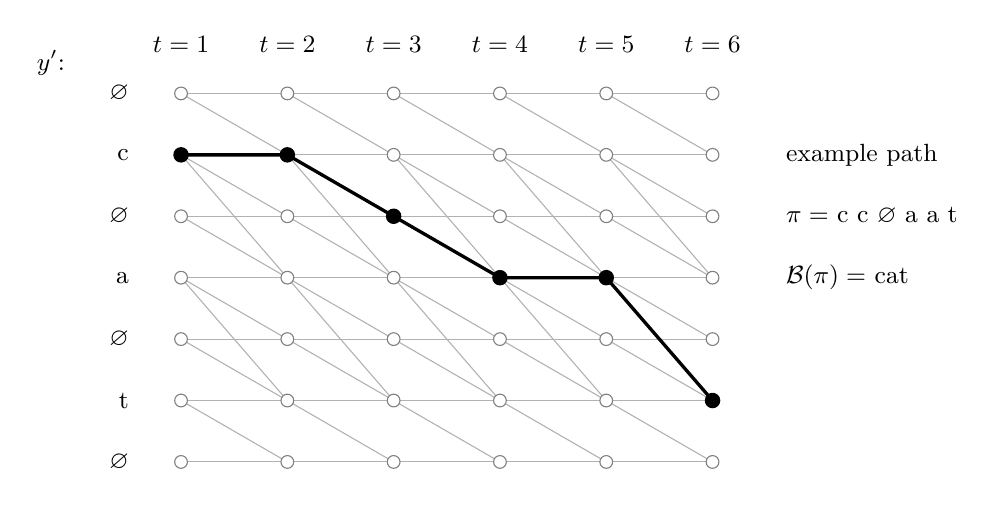
\begin{tikzpicture}[x={(1.35cm,0)},y={(0,-0.78cm)}]
\foreach \t in {1,...,5} {
  \foreach \s in {1,...,7} {\draw[gray!60] (\t,\s) -- (\t+1,\s);}
  \foreach \s in {1,...,6} {\draw[gray!60] (\t,\s) -- (\t+1,\s+1);}
  \draw[gray!60] (\t,2) -- (\t+1,4);
  \draw[gray!60] (\t,4) -- (\t+1,6);
}
\foreach \t in {1,...,6} {\foreach \s in {1,...,7} {\fill[white,draw=gray] (\t,\s) circle (2.3pt);}}
\foreach \s/\l in {1/$\varnothing$,2/c,3/$\varnothing$,4/a,5/$\varnothing$,6/t,7/$\varnothing$} {\node[font=\small,anchor=east] at (0.6,\s) {\l};}
\foreach \t in {1,...,6} {\node[font=\small,anchor=south] at (\t,0.5) {$t=\t$};}
\draw[very thick] (1,2) -- (2,2) -- (3,3) -- (4,4) -- (5,4) -- (6,6);
\foreach \t/\s in {1/2,2/2,3/3,4/4,5/4,6/6} {\fill (\t,\s) circle (2.8pt);}
\node[font=\small,anchor=west] at (6.6,2) {example path};
\node[font=\small,anchor=west] at (6.6,3) {$\pi=$ c c $\varnothing$ a a t};
\node[font=\small,anchor=west] at (6.6,4) {$\mathcal B(\pi)=$ cat};
\node[font=\small,anchor=east] at (0.0,0.5) {$y'$:};
\end{tikzpicture}
\caption{CTC lattice for the word ``cat'' with $T=6$ steps. The rows are the positions of the blank-augmented label $y'$; thin lines are the allowed transitions of Equation~\ref{eq:rec-alpha} (stay, advance, and skip over a blank between different letters). The thick path is one of the many paths that collapse to the word.}
\label{fig:rec-ctc}
\end{figure}

Three conventions of the implementation of Equations~\ref{eq:rec-ctcprob} to~\ref{eq:rec-ctcgrad} matter for the losses quoted below.
Each line's loss is divided by its target length, so every loss quoted below is a per-character negative log-likelihood, and lines with no valid path are given zero loss.
Every line of a batch uses the full $T=160$ steps including the padding.
A label cap of 120 characters, $\lfloor160\cdot0.75\rfloor$, keeps every label far below $T$, which CTC requires: it needs $T\ge U$ plus the number of adjacent repeated letters of the target.


\paragraph{Decoding.}
At inference the most probable symbol of each step is taken, repeats are merged and blanks deleted, which is the best-path (greedy) decoding of Graves \emph{et al.}~\cite{graves2006}, Equation~\ref{eq:rec-greedy}:
\begin{equation}
\hat\pi_t=\arg\max_k y_t^k,\qquad \hat y=\mathcal B(\hat\pi).
\label{eq:rec-greedy}
\end{equation}
In Equation~\ref{eq:rec-greedy}, $y_t^k$ is the probability of class $k$ at step $t$, $\hat\pi$ the path of per-step arg-maxima and $\mathcal B$ the many-to-one map defined above that merges repeats and deletes blanks.
This best-path decoding approximates $\arg\max_y p(y\mid x)$ in 160 arg-max operations; no lexicon, language model or beam search is used.
The published design reaches its best error rate with lexicon-constrained decoding, which was not implemented here, so that publication's headline figure is not a result of this project.

\subsubsection{Training data and splits}

Table~\ref{tab:rec-data} lists the data sets, the rule separating training from validation data, and the leakage each rule leaves.

\begin{table}[h]
\centering
\fontsize{9.5}{11.5}\selectfont
\begin{tabularx}{\linewidth}{|p{2.8cm}|p{3.6cm}|X|}
\hline
\textbf{Data set} & \textbf{Split rule} & \textbf{Caveat on the validation figure} \\
\hline
Lines segmented by the student's own block from scanned database pages, with labels generated by alignment (first stage only) &
The last labelled page of every writer is held out. &
Same writers in training and hold-out, so the figure is writer-dependent; the labels are project-generated and noisy. \\
\hline
Public line-level IAM transcription set: 6\,482 training, 976 validation, 2\,915 test lines (6\,481, 976 and 2\,915 after label cleaning) &
Official training, validation and test partitions. &
The validation set drives learning-rate decay and checkpoint choice, so its accuracy is mildly optimistic; the test set is used for no decision. The partitions are believed, but not verified, to be writer-independent, and the warm start from the first stage may have seen some of the same forms. \\
\hline
13 photographed pages of the two personal writers (8 and 5 pages), 355 transcription lines of which one is a diagram marker. \mustdo{This row describes the two-writer personal set. The project now has five personal writers, 30 photographed pages and 669 transcription lines, and Section~\ref{sec:results} reports the recogniser's accuracy on all 669 of them while stating that those writers appear in its fine-tuning data. Confirm which personal set the deployed recogniser was actually fine-tuned on, and correct this row and the one below to match. I could not establish this from the saved checkpoints.} &
Per page, 15\,\% of the lines (at least one) are drawn at random with a fixed seed as validation; about 52 validation lines in total. &
Validation lines come from the same pages, pen, paper, lighting and vocabulary as training lines; the figure measures ``same writer, same notebook, new lines'' and is optimistic. It also takes part in checkpoint selection. \\
\hline
Ten-author hold-out (eight database writers and two of the personal writers) &
Used only as an evaluation set. &
The held-out database lines may have been seen in the line-level training data, and their labels are project-generated, so the figure is not a writer-independent measure. \\
\hline
\end{tabularx}
\caption{Data sets of the text recogniser and their leakage assessment.}
\label{tab:rec-data}
\end{table}

In short, the first-stage hold-out is writer-dependent with noisy labels; the public set's validation split drives learning-rate decay and checkpoint choice, so its accuracy is mildly optimistic, while its test split is used for no decision, although the partitions are only believed, not verified, to be writer-independent; the personal validation lines are random lines of the same pages as the training lines (optimistic); and the ten-author hold-out may overlap the training data and has project-generated labels.
The labels of the database pages were generated by aligning the printed prompt words with the detected ink word runs by dynamic programming, the Needleman--Wunsch global alignment~\cite{needleman1970} with the project's own cost. An earlier purely proportional labelling assigned wrong text to lines; correcting the evaluation labels, with no change of the weights, raised the measured accuracy on the ten-author hold-out from 42.7\,\% to 89.4\,\%.
Label quality, not the network, had limited the earlier measurements, which is why the recogniser was later trained on a public line-level set with clean labels.

\paragraph{Data augmentation.}
Training images, and never validation images, are augmented after the resize to $64\times640$ with at most one of four geometric transformations: horizontal shear, rotation, elastic distortion~\cite{simard2003} and perspective distortion.
Each of the four is enabled independently with probability 0.5; if none is enabled the image is unchanged, otherwise one of the enabled ones is chosen uniformly, so that $P(\text{no augmentation})=1/16=6.25\,\%$ and at most one transformation acts on an image.
The transformations are a horizontal \emph{shear} with factor $k\sim U(-0.6,0.6)$ (angle $\arctan k$), a \emph{rotation} by an angle in $U(-2.5^\circ,2.5^\circ)$, an \emph{elastic distortion}~\cite{simard2003} in which random displacement fields (uniform in $[-1,1]$ per pixel) are smoothed with a Gaussian of standard deviation $\sigma\in\{3,4\}$ and scaled by $\alpha\in\{15,20\}$ before the image is warped, and a \emph{perspective} distortion in which each corner is moved by up to $d\,W/2$ horizontally and $d\,H/2$ vertically with $d\sim U(0.03,0.08)$, where $W$ and $H$ are the canvas width and height.
The fill colour of the geometric transformations is white.
No colour, contrast, noise or blur augmentation and no synthetic pre-training data are used.

\subsubsection{Training procedure}

\paragraph{Optimiser.}
The loss of Equation~\ref{eq:rec-ctcprob} is minimised by mini-batch gradient descent with the RMSprop update of Tieleman and Hinton~\cite{tieleman2012}, Equation~\ref{eq:rec-rmsprop}: for the gradient $g_t$ at update $t$, learning rate $\eta$ and weight decay $\lambda=10^{-5}$ (an L2 term added to the gradient), the update is
\begin{equation}
g_t\leftarrow g_t+\lambda\theta_{t-1},\qquad v_t=\rho\,v_{t-1}+(1-\rho)\,g_t^2,\qquad \theta_t=\theta_{t-1}-\eta\,\frac{g_t}{\sqrt{v_t}+\epsilon},
\label{eq:rec-rmsprop}
\end{equation}
with $\theta$ the parameters, $v_t$ the running average of the squared gradient (smoothing $\rho=0.99$) and $\epsilon=10^{-8}$; there is no momentum in Equation~\ref{eq:rec-rmsprop}.
Dividing the step by the square root of that running average gives every parameter its own step size, which suits the very different gradient magnitudes of convolutional and recurrent layers.
In the joint stage the global gradient norm is clipped at 5 by the rule of Pascanu \emph{et al.}~\cite{pascanu2013}, Equation~\ref{eq:rec-clip},
\begin{equation}
g\leftarrow g\,\min\Bigl(1,\frac{5}{\|g\|_2}\Bigr),
\label{eq:rec-clip}
\end{equation}
$g$ being the concatenated gradient of all parameters and $\|g\|_2$ its Euclidean norm; the clip of Equation~\ref{eq:rec-clip} stops a rare exploding gradient of the recurrent layers from destroying the weights, and batches with a non-finite loss are skipped.
A plateau schedule halves the learning rate: after a number of validation checks (the patience) without improvement of the validation loss, $\eta\leftarrow\max(0.5\,\eta,\eta_{\min})$, with $\eta$ the learning rate of Equation~\ref{eq:rec-rmsprop} and $\eta_{\min}$ a floor below which it is not reduced.
The patience of each stage, its floor $\eta_{\min}$ (which was $10^{-5}$ or $10^{-6}$) and its restart rule are listed in Table~\ref{tab:rec-stages}.

\paragraph{Staged recipe.}
Training was carried out in four stages (Table~\ref{tab:rec-stages}, Figure~\ref{fig:rec-stages}), and each stage is motivated by a limitation that was found in the previous one.
\begin{enumerate}
\item \emph{Base stage.} The published recipe was reproduced on lines that were segmented from database pages by the student's own tools. The data turned out to be small and noisy because of the labelling defect and segmentation errors, and the best validation loss was 1.06.
\item \emph{Clean-label stage.} The network was warm-started from the base stage and trained on the public line-level IAM set, whose human-checked labels remove all segmentation and labelling noise.
\item \emph{Personal fine-tuning (rejected).} Fine-tuning on the personal lines alone raised the accuracy on the personal validation lines but reduced the accuracy on the general data by about ten points (catastrophic forgetting, Table~\ref{tab:rec-forget}); freezing the convolutional layers reduced the forgetting only slightly.
\item \emph{Joint stage.} Training continues from the clean-label stage on both data sets at once, with a weighted sampler: each public line receives the weight $w_T=(1-f)/n_T$ and each personal line $w_P=f/n_P$, where $n_T=6\,481$, $n_P\approx280$ and $f=0.20$, and $n_T$ indices are drawn per epoch with replacement with probability proportional to the weights, Equation~\ref{eq:rec-sampler},
\begin{equation}
P(i)=\frac{w_i}{\sum_jw_j}.
\label{eq:rec-sampler}
\end{equation}
In expectation the sampler of Equation~\ref{eq:rec-sampler} draws 20\,\% of every epoch ($\approx1\,296$ draws) from the personal set, so that each personal line is seen about 4.6 times per epoch with fresh random augmentation, and 80\,\% from the public set. The checkpoint of the epoch with the largest $\min(\text{accuracy}_{\mathrm{public}},\text{accuracy}_{\mathrm{personal}})$ is kept, so that neither domain is sacrificed. This stage wrote the checkpoint file \texttt{paper\_cnn\_bilstm\_ctc\_joint\_best.npz}, which is the file every accuracy quoted for stage~4 was measured on.
\end{enumerate}

\begin{table}[h]
\centering
\fontsize{9.5}{11.5}\selectfont
\begin{tabularx}{\linewidth}{|l|l|l|l|l|l|X|}
\hline
\textbf{Stage} & \textbf{Data} & \textbf{$\eta_0$} & \textbf{Batch} & \textbf{Epochs} & \textbf{Clip} & \textbf{Schedule and selection} \\
\hline
Base & own lines & $10^{-3}$ & 16 & $\le200$ & none & halve after 5 stalls; stop after 15; up to 3 restarts from the best weights; best validation loss \\
\hline
Clean labels & public set & $10^{-3}$ & 16 & $\le200$ & none & as above, up to 8 restarts; best public validation loss \\
\hline
Personal & personal lines & $3\!\times\!10^{-4}$ & 8 & 60 & 5 & halve after 5 stalls; best personal validation loss \\
\hline
Joint & both, $f=0.20$ & $5\!\times\!10^{-4}$ & 16 & 30 & 5 & halve after 4 stalls on the sum of both validation losses; best $\min$ of the two accuracies \\
\hline
\end{tabularx}
\caption{Hyper-parameters of the four training stages. All stages use RMSprop~\cite{tieleman2012} (Equation~\ref{eq:rec-rmsprop}) with weight decay $10^{-5}$; the minimum learning rate was $10^{-5}$ or $10^{-6}$.}
\label{tab:rec-stages}
\end{table}

\begin{figure}[h]
\centering
\begin{tikzpicture}[x=1cm,y=1cm]
\tikzset{sb/.style={w2box,text width=3.6cm,minimum height=1.4cm}}
\node[sb] (b) at (-5.4,0) {\textbf{1 Base}\\ own database lines, noisy labels\\ best val. loss 1.06};
\node[sb] (h) at (-0.6,0) {\textbf{2 Clean labels}\\ public line set, 6\,481 lines\\ val./test 93.87/91.60\,\%};
\node[sb] (n) at (4.5,1.2) {\textbf{3 Personal only (rejected)}\\ val./test 84.26/80.56\,\%\\ personal 90.2\,\%};
\node[sb] (j) at (4.5,-1.2) {\textbf{4 Joint, 80/20 sampler}\\ val./test 94.03/91.82\,\%\\ personal 89.64\,\%};
\draw[w2arr] (b)--(h) node[midway,above,font=\scriptsize] {warm start};
\draw[w2arr] (h.east) -- ++(0.45,0) |- (n.west);
\draw[w2arr] (h.east) -- ++(0.45,0) |- (j.west);
\end{tikzpicture}
\caption{Staged training recipe of the text recogniser with the character accuracies (public validation and test sets, and personal validation; see Table~\ref{tab:rec-results} for the caveats). Stage~2 wrote \texttt{paper\_cnn\_bilstm\_ctc\_hf\_best.npz}, stage~3 \texttt{paper\_cnn\_bilstm\_ctc\_personal\_best.npz} and stage~4 \texttt{paper\_cnn\_bilstm\_ctc\_joint\_best.npz}; every accuracy in the figure was measured on the stage's own file. The checkpoint the deployed server actually loads is a different, later one, \texttt{paper\_cnn\_bilstm\_ctc\_scratch\_best.npz}, for which no accuracy is reported anywhere in this report (see below).}
\label{fig:rec-stages}
\end{figure}

Table~\ref{tab:rec-forget} sets the three ways of adding the personal data side by side.

\begin{table}[h]
\centering
\fontsize{9.5}{11.5}\selectfont
\begin{tabular}{|l|r|r|r|}
\hline
\textbf{Training} & \textbf{Public val./test (\%)} & \textbf{Personal val. (\%)} & \textbf{Remark} \\
\hline
Clean-label stage only & 93.87 / 91.60 & -- & before personal data \\
Personal only, all layers & 84.26 / 80.56 & 90.2 & forgetting \\
Personal only, frozen convolutions & 85.87 / 82.62 & 88.5 & forgetting \\
Joint, 80/20 sampler & 94.03 / 91.82 & 89.64 & both domains kept \\
\hline
\end{tabular}
\caption{The catastrophic-forgetting experiment: character accuracies of the three ways of adding personal data. Every figure in the table was measured on the stage's own checkpoint file, the last row on \texttt{paper\_cnn\_bilstm\_ctc\_joint\_best.npz}; none of them was measured on the from-scratch checkpoint that the server loads.}
\label{tab:rec-forget}
\end{table}

\paragraph{Which checkpoint is deployed.}
Four text checkpoints exist in \texttt{Software/CNN/weights}, and the quoted accuracies belong to three of them: \texttt{paper\_cnn\_bilstm\_ctc\_hf\_best.npz} from the clean-label stage (93.87\,\% public validation, 91.60\,\% public test), \texttt{paper\_cnn\_bilstm\_ctc\_personal\_best.npz} from the rejected personal-only stage (84.26/80.56\,\% public, 90.2\,\% personal) and \texttt{paper\_cnn\_bilstm\_ctc\_joint\_best.npz} from the joint stage (94.03/91.82\,\% public, 89.64\,\% personal), the figures of Table~\ref{tab:rec-forget} and Figure~\ref{fig:rec-stages}.
The fourth file, \texttt{paper\_cnn\_bilstm\_ctc\_scratch\_best.npz}, is the output of the from-scratch trainer of Section~\ref{sec:textrec-numpynn}, and it is the file the deployed system actually uses: the loader prefers it over the joint checkpoint whenever it exists, which it does, so the server serves the from-scratch weights and not the joint ones.
This matters for every accuracy in this subsection, because no accuracy of the from-scratch checkpoint is reported anywhere in this report.
Its training produced no log, and unlike the resumable runs described below its stored file contains weights and batch-normalisation statistics only, with no epoch number and no best validation score, so neither its selected epoch nor its accuracy can be recovered from the file.
The honest position is therefore that the four-stage recipe and its accuracies describe the joint checkpoint, while the deployed path loads a later checkpoint of the same architecture whose accuracy has not been measured.
\mustdo{resolve the checkpoint question before submission: either re-run the evaluation of Table~\ref{tab:rec-results} on \texttt{paper\_cnn\_bilstm\_ctc\_scratch\_best.npz} and quote its public validation, public test and personal-crop accuracies beside the joint figures, or state explicitly which single checkpoint is being submitted as the deployed recogniser and remove the other from the loader's search path so that the quoted figures and the served weights are the same file.}

A sweep over learning rate, LSTM width, depth, convolution width, dropout and optimiser (14 configurations of 50 epochs) was programmed, but no result file was kept, so the deployed architecture is the published one and not an optimum found by the student.
Training was done offline on a general-purpose computer; the training log of the joint stage was not kept, so epoch-by-epoch curves cannot be shown, and the stored joint checkpoint contains weights only.

\subsubsection{From-scratch forward-and-backward implementation}
\label{sec:textrec-numpynn}

Only work done from first principles counts for credit in this report, so a framework supplying ready-made layers and automatic differentiation would earn no credit for the recogniser's training.
The student therefore wrote one Python module that implements, from the defining equations and with no machine-learning library, the forward \emph{and} the backward (gradient) pass of every layer used by the recogniser and the two writer classifiers of Section~\ref{sec:writerid}, together with the two optimiser updates, the learning-rate schedules and the gradient-norm clip, so that no machine-learning framework supplies any layer, any gradient or any optimiser used in training.
The scope of that claim is stated precisely at the end of this subsection: it is a claim about the learning machinery, not a claim that the training programs import nothing at all.

\paragraph{Layers implemented from first principles.}
The module implements, from the defining equations and with no machine-learning library, the forward and the backward pass of the convolution of Equation~\ref{eq:rec-conv}, batch normalisation in its training form (batch statistics, Equation~\ref{eq:rec-bn}) and its folded inference form (Equation~\ref{eq:rec-bnfold}), the rectified linear unit, max-pooling and the two adaptive pools of Equations~\ref{eq:rec-hmax} and~\ref{eq:wid-pool}, a fully connected (linear) layer, dropout, the multilayer bidirectional LSTM of Equations~\ref{eq:rec-lstm} and~\ref{eq:rec-bi}, and the CTC forward--backward recursion of Equations~\ref{eq:rec-alpha} to~\ref{eq:rec-ctcgrad}.
It also implements the RMSprop update of Equation~\ref{eq:rec-rmsprop}, the AdamW update of the writer classifiers (Equations~\ref{eq:wid-adamwmom} and~\ref{eq:wid-adamw}), the plateau and cosine learning-rate schedules and the gradient-norm clip of Equation~\ref{eq:rec-clip}, so that no layer, no gradient and no optimiser update used in training comes from a machine-learning framework.
One shared training program calls it to build and train either the recogniser or a writer classifier, since the two share the convolutional backbone (Section~\ref{sec:writerid}).
The convolutional stack, the pooling layers and the fully connected layer are also called in their inference (eval) form by the validation step at the end of every epoch and by the deployed program on the single-board computer, so training, validation and deployment are three uses of one implementation.
The framework alternative would have earned no credit for the recogniser's training even though the student designed the architecture and data pipeline around it.

\paragraph{Exactly what the training code does and does not import.}
The claim made above is deliberately narrower than ``no external library at all'', because the latter would not be true, and the difference is worth stating exactly.
Every layer forward pass, every backward pass, both optimisers, both learning-rate schedules and the gradient-norm clip are in the student's own module \texttt{NumpyNN.py}, which imports nothing but \texttt{numpy}; the module contains no machine-learning import of any kind, and the from-scratch trainer builds and trains both the recogniser and the writer classifiers out of it alone.
The data pipeline that feeds that trainer does use two image-processing utilities from SciPy, and only two.
The first is \texttt{scipy.ndimage}, from which \texttt{gaussian\_filter} and \texttt{map\_coordinates} are imported at \texttt{Software/CleanPipeline/TrainText.py:27} and used to smooth the random displacement fields and to resample the warped image in the elastic distortion described above (\texttt{TrainText.py:175--180}); an equivalent separable Gaussian blur and bilinear resampling could have been written from the definitions already given in this report (Equation~\ref{eq:rec-resize} supplies the interpolation), and that they were not is a convenience and not a dependence of the learning algorithm.
The second is \texttt{scipy.signal.find\_peaks}, imported at \texttt{Software/CleanPipeline/ExtractIAMLines.py:12} and used once, to locate the minima of the smoothed row-ink profile when lines are cut out of a database page.
The from-scratch trainer \texttt{TrainScratch.py} reuses the data loaders of \texttt{TrainText.py} and \texttt{TrainAuthor.py} and therefore inherits both of these, and it also depends on the Python imaging library for reading and resizing image files.
Neither utility touches a weight, a gradient or an update: elastic distortion acts on the input image before Equation~\ref{eq:rec-norm}, and peak finding acts on a page before any line exists.
The defensible statement, and the one this report makes, is therefore that \emph{no machine-learning framework supplies any layer, gradient or optimiser}, while two SciPy image-processing utilities (Gaussian smoothing with resampling for the elastic augmentation, and peak finding for line cutting) and the imaging library are used in the data pipeline around the network.
One further library, the data-set reader used by \texttt{ExportTekliaLines.py} to export the public line images once to disk, is used outside training altogether and never during it.

\paragraph{Backward passes derived by hand.}
The forward equations of every layer have been given above; this paragraph gives the backward equations that go with them, because it is the backward passes, and not the forward ones, that a framework would otherwise have supplied, and a gradient that is merely exhibited as code has not been derived.
Throughout, $\mathcal L$ is the scalar loss and, for a tensor $A$ appearing in a forward equation, $\mathrm dA$ denotes the tensor of partial derivatives $\partial\mathcal L/\partial A$, of the same shape as $A$; $\mathrm dA$ is precisely what the module's backward function for that layer returns to its caller, $\mathrm dY$ is the gradient arriving from the layer above, $\odot$ is the element-wise product and $\mathbb 1[\cdot]$ the indicator function.
Each equation below is checked by one or more configurations of the numerical check of the next paragraph, and the correspondence between the two is stated there.

\emph{Two-dimensional convolution.} Differentiating the forward sum of Equation~\ref{eq:rec-conv} with respect to its three arguments gives
$\mathrm dW[o,c,u,v]=\sum_{n,i,j}\mathrm dY[n,o,i,j]\,X_{\mathrm{pad}}[n,c,si+u,sj+v]$ for the weights,
a plain sum over batch and position for the bias, and a sum over every window in which a given input pixel appears for the input.
Since the column of $\mathrm{cols}_n$ indexed by the output position $(i,j)$ holds exactly those entries $X_{\mathrm{pad}}[n,c,si+u,sj+v]$ for all $(c,u,v)$, the first of these is a matrix product, and the implementation evaluates the three gradients of Equation~\ref{eq:rec-im2col} as Equation~\ref{eq:rec-convbw},
\begin{equation}
\mathrm d\tilde W=\sum_{n=1}^{B}\mathrm dY_n\,\mathrm{cols}_n^{\top},\qquad
\mathrm db_o=\sum_{n,i,j}\mathrm dY[n,o,i,j],\qquad
\mathrm d\,\mathrm{cols}_n=\tilde W^{\top}\,\mathrm dY_n,
\label{eq:rec-convbw}
\end{equation}
in which the sum for $\mathrm db_o$ runs over the batch and over all $H_{\mathrm{out}}W_{\mathrm{out}}$ output positions, $B$ is the batch size, $\mathrm dY_n\in\mathbb R^{C_{\mathrm{out}}\times H_{\mathrm{out}}W_{\mathrm{out}}}$ is the incoming gradient of sample $n$ with its two spatial axes flattened, $\mathrm{cols}_n$ is that sample's im2col matrix from Equation~\ref{eq:rec-im2col}, $\tilde W\in\mathbb R^{C_{\mathrm{out}}\times C_{\mathrm{in}}k^2}$ is the reshaped weight matrix of Equation~\ref{eq:rec-im2col}, and $\mathrm d\tilde W$ is reshaped back to the four axes of $W$ before it is returned.
Both products of Equation~\ref{eq:rec-convbw} are evaluated as one batched product over $n$ (the sum over the batch being a reduction of the leading axis of the first), which is the saving quantified in Figure~\ref{fig:rec-conv2d}; the three gradients are the exact derivative of Equation~\ref{eq:rec-conv} and not an approximation of it, since Equation~\ref{eq:rec-im2col} is Equation~\ref{eq:rec-conv} rearranged.
The input gradient is then returned from the columns to the image by the col2im operation of Equation~\ref{eq:rec-col2im},
\begin{equation}
\begin{gathered}
\mathrm dX_{\mathrm{pad}}[n,c,r,q]=\sum_{u=0}^{k-1}\sum_{v=0}^{k-1}\mathrm d\,\mathrm{cols}\bigl[n,\,(c,u,v),\,(r-u,\;q-v)\bigr],\\
\mathrm dX=\mathrm dX_{\mathrm{pad}}\bigl[\,\cdot\,,\,\cdot\,,\;p{:}p{+}H,\;p{:}p{+}W\,\bigr],
\end{gathered}
\label{eq:rec-col2im}
\end{equation}
where $(r,q)$ is a position of the zero-padded input, $(c,u,v)$ indexes the rows of $\mathrm{cols}$ as channel and kernel offset, terms whose output index $(r-u,q-v)$ falls outside the $H_{\mathrm{out}}\times W_{\mathrm{out}}$ grid are zero, and the second expression of Equation~\ref{eq:rec-col2im} discards the $p$-pixel border that padding added, recovering a gradient of the same shape as the layer's input.
Equation~\ref{eq:rec-col2im} is the transpose of the im2col rearrangement and it must \emph{accumulate}: for $k>1$ the windows overlap, so one input pixel appears in up to $k^2=9$ columns and receives one contribution from each.
The implementation therefore realises it as a scatter-add, a loop of nine slice additions into a zero-initialised padded array; a reshape alone, which would be correct for non-overlapping windows, would here keep one contribution in nine and is the single most likely place for a convolution backward pass to be silently wrong.

\emph{Batch normalisation in its training form.} The learned parameters of Equation~\ref{eq:rec-bn} differentiate immediately, as Equation~\ref{eq:rec-bnbw},
\begin{equation}
\mathrm d\gamma_c=\sum_{n,i,j}\mathrm dY[n,c,i,j]\,\hat x[n,c,i,j],\qquad
\mathrm d\beta_c=\sum_{n,i,j}\mathrm dY[n,c,i,j],\qquad
\mathrm d\hat x=\gamma_c\,\mathrm dY,
\label{eq:rec-bnbw}
\end{equation}
where $\hat x$ is the normalised activation of Equation~\ref{eq:rec-bn}, $\gamma_c$ and $\beta_c$ the scale and shift of channel $c$, and every sum runs over the batch index $n$ and both spatial axes $(i,j)$ of that channel.
The input gradient is harder, because the mean $\mu_B$ and the variance $\sigma_B^2$ of Equation~\ref{eq:rec-bn} are themselves functions of every element of the channel: perturbing one element changes the output through three routes, directly through $\hat x$, through $\mu_B$ and through $\sigma_B^2$.
Collecting the three routes gives the single expression of Equation~\ref{eq:rec-bnbwx}, the form the module implements,
\begin{equation}
\mathrm dx=\frac{1}{N\sqrt{\sigma_B^2+\varepsilon}}\Bigl(N\,\mathrm d\hat x\;-\;\sum_{n,i,j}\mathrm d\hat x\;-\;\hat x\sum_{n,i,j}\bigl(\mathrm d\hat x\odot\hat x\bigr)\Bigr),
\label{eq:rec-bnbwx}
\end{equation}
in which $N=BHW$ is the number of elements of the channel over which Equation~\ref{eq:rec-bn} takes its statistics, $\varepsilon=10^{-5}$, and the two sums are scalars per channel that are broadcast back over all $N$ positions.
The three terms of Equation~\ref{eq:rec-bnbwx} are the three routes in order, and the two sums are what couples all $N$ elements of a channel: training-form batch normalisation is the one layer in this network whose backward pass cannot be written element by element, and Equation~\ref{eq:rec-bnbwx} computes all $N$ derivatives in one pass over the channel instead of $N$ separate ones.
Equation~\ref{eq:rec-bnbwx}, and not the folded inference map of Equation~\ref{eq:rec-bnfold}, is the form that is differentiated, because the folded form is never trained through: the running statistics receive no gradient at all, being updated outside the gradient path by $\mu_{\mathrm{run}}\leftarrow(1-m)\mu_{\mathrm{run}}+m\,\mu_B$ with momentum $m=0.1$, the variance by its unbiased estimate $\sigma_B^2N/(N-1)$.

\emph{Rectified linear unit and dropout.} Both are masks, and both backward passes re-apply the mask the forward pass recorded, Equation~\ref{eq:rec-relubw}:
\begin{equation}
\mathrm dx=\mathrm dY\odot\mathbb 1[x>0]\quad\text{(rectifier)},\qquad
\mathrm dx=\mathrm dY\odot M,\quad M_k=\frac{\mathbb 1[\xi_k\ge p]}{1-p}\quad\text{(dropout)},
\label{eq:rec-relubw}
\end{equation}
where $x$ is the rectifier's input, $M$ the inverted-dropout mask of Equation~\ref{eq:wid-head} with keep probability $1-p$ and $\xi_k$ the uniform draw of unit $k$.
The kink of the rectifier at $x=0$ is assigned the derivative zero in Equation~\ref{eq:rec-relubw}, which is the usual convention and is the reason the numerical check of that layer is run on inputs that keep every element away from the kink.

\emph{Max-pooling and the two adaptive pools.} A maximum is a selector, so it routes the whole incoming gradient to the element that won and nothing to the others, Equation~\ref{eq:rec-poolbw}:
\begin{equation}
\mathrm dX[n,c,2i+u,2j+v]=\begin{cases}\mathrm dY[n,c,i,j], & (u,v)=a^{\star}(n,c,i,j),\\[2pt] 0,&\text{otherwise,}\end{cases}
\label{eq:rec-poolbw}
\end{equation}
with $a^{\star}(n,c,i,j)=\arg\max_{u,v\in\{0,1\}}X[n,c,2i+u,2j+v]$ the within-window arg-max that the forward pass of the $2\times2$ pool stored in its cache, and $u,v\in\{0,1\}$ ranging over the window of output position $(i,j)$.
Because the stride equals the kernel, the windows of Equation~\ref{eq:rec-poolbw} tile the input without overlapping, so the routed values can be written into place directly and, unlike Equation~\ref{eq:rec-col2im}, no accumulation is needed.
The height maximum of Equation~\ref{eq:rec-hmax} and the width mean of Equation~\ref{eq:wid-pool} differentiate to the two halves of Equation~\ref{eq:rec-adaptbw},
\begin{equation}
\begin{gathered}
\mathrm dF[n,c,i,t]=\mathbb 1\bigl[\,i=r^{\star}(n,c,t)\,\bigr]\,\mathrm dz_t[n,c],\qquad r^{\star}(n,c,t)=\arg\max_iF[n,c,i,t],\\
\mathrm dm[n,c,t]=\frac{1}{T}\,\mathrm df[n,c],
\end{gathered}
\label{eq:rec-adaptbw}
\end{equation}
where $r^{\star}$ is the winning row cached by the forward pass of Equation~\ref{eq:rec-hmax} and $T=160$ the number of columns the mean of Equation~\ref{eq:wid-pool} runs over.
The first half of Equation~\ref{eq:rec-adaptbw} sends the gradient of a time step to the one row that supplied its value, so a feature that is never the column maximum receives nothing, which is the gradient-side price of discarding vertical position in Equation~\ref{eq:rec-hmax}.
The second half spreads the gradient of a pooled feature evenly over all 160 columns including the white padding of a short line, the exact counterpart of the dilution noted after Equation~\ref{eq:wid-pool}.

\emph{Fully connected layer.} With every axis but the last flattened into one index, Equation~\ref{eq:rec-linbw} holds:
\begin{equation}
\mathrm dW=\mathrm dY^{\top}X,\qquad \mathrm db=\sum_{m=1}^{M}\mathrm dY[m,\,\cdot\,],\qquad \mathrm dX=\mathrm dY\,W,
\label{eq:rec-linbw}
\end{equation}
where $X\in\mathbb R^{M\times I}$ is the input and $\mathrm dY\in\mathbb R^{M\times O}$ the incoming gradient with all leading axes collapsed into the index $m$, $W\in\mathbb R^{O\times I}$ is the weight matrix and $\mathrm dX$ is reshaped back to the input's own axes before it is returned.
That flattening is what lets one function serve both uses of the layer without change: for the recogniser's output layer of Equation~\ref{eq:rec-softmax}, $M=TB=160B$, so all 160 time steps of all lines of a batch contribute to one weight gradient, whereas for the writer classifier's head of Equation~\ref{eq:wid-head}, $M=B$.

\emph{Long short-term memory.} At step $t$ the hidden state is reached both from the layer above and from step $t+1$, and the memory only from step $t+1$, so the two gradients entering the cell are $\mathrm dh_t=\mathrm dY_t+\delta h_t$ and $\mathrm dc_t=\delta c_t+\mathrm dh_t\odot o_t\odot(1-\tanh^2c_t)$, where $\mathrm dY_t$ is the gradient of $h_t$ from above, $\delta h_t$ and $\delta c_t$ are the recurrent contributions produced by step $t+1$, and both recurrent terms are zero at $t=T$.
Differentiating the six lines of Equation~\ref{eq:rec-lstm} with $\sigma'=\sigma(1-\sigma)$ and $\tanh'=1-\tanh^2$ gives the four gate pre-activation gradients of Equation~\ref{eq:rec-lstmbw},
\begin{equation}
\begin{aligned}
\mathrm d\tilde o_t&=\mathrm dh_t\odot\tanh(c_t)\odot o_t\odot(1-o_t), &\qquad \mathrm d\tilde f_t&=\mathrm dc_t\odot c_{t-1}\odot f_t\odot(1-f_t),\\
\mathrm d\tilde i_t&=\mathrm dc_t\odot g_t\odot i_t\odot(1-i_t), &\qquad \mathrm d\tilde g_t&=\mathrm dc_t\odot i_t\odot(1-g_t^2),
\end{aligned}
\label{eq:rec-lstmbw}
\end{equation}
in which a tilde marks a gate's pre-activation, that is the argument of the $\sigma$ or $\tanh$ in Equation~\ref{eq:rec-lstm}, and $i_t$, $f_t$, $g_t$, $o_t$, $c_{t-1}$ and $\tanh(c_t)$ are the activations the forward pass cached at that step; each line of Equation~\ref{eq:rec-lstmbw} is the gradient of the cell output with respect to one gate multiplied by that gate's own activation derivative, so the forward cache makes the backward pass free of any re-evaluation.
The recursion that carries Equation~\ref{eq:rec-lstmbw} through time, the back-propagation through time proper, is Equation~\ref{eq:rec-lstmbptt},
\begin{equation}
\begin{aligned}
\mathrm d\tilde a_t&=\bigl[\,\mathrm d\tilde i_t;\;\mathrm d\tilde f_t;\;\mathrm d\tilde g_t;\;\mathrm d\tilde o_t\,\bigr]\in\mathbb R^{B\times4n},\\
\delta h_{t-1}&=\mathrm d\tilde a_t\,W_{hh},\qquad \delta c_{t-1}=\mathrm dc_t\odot f_t,\qquad \mathrm dx_t=\mathrm d\tilde a_t\,W_{ih},\\
\mathrm dW_{ih}&=\sum_{t=1}^{T}\mathrm d\tilde a_t^{\top}x_t,\qquad \mathrm dW_{hh}=\sum_{t=1}^{T}\mathrm d\tilde a_t^{\top}h_{t-1},\qquad \mathrm db_{ih}=\mathrm db_{hh}=\sum_{t=1}^{T}\mathbf 1^{\top}\mathrm d\tilde a_t,
\end{aligned}
\label{eq:rec-lstmbptt}
\end{equation}
with $n=256$ the hidden size, $W_{ih}\in\mathbb R^{4n\times I}$ and $W_{hh}\in\mathbb R^{4n\times n}$ the stacked gate matrices introduced after Equation~\ref{eq:rec-lstm}, $\mathrm d\tilde a_t$ the four gate gradients stacked in the same gate order, and $\mathbf 1^{\top}\mathrm d\tilde a_t$ the sum over the $B$ samples of the batch.
The loop of Equation~\ref{eq:rec-lstmbptt} runs from $t=T$ down to $t=1$, carries $\delta h_{t-1}$ and $\delta c_{t-1}$ into the previous step, accumulates the four parameter gradients over all 160 steps and emits $\mathrm dx_t$ for the layer below; the single concatenated $\mathrm d\tilde a_t$ mirrors the single concatenated forward product, so a step costs two matrix products of $4n=1024$ rows backwards against one forwards.
Both bias gradients of Equation~\ref{eq:rec-lstmbptt} are equal because both biases enter the same pre-activation sum in Equation~\ref{eq:rec-lstm}, a redundancy kept so that the checkpoint format matches the four-tensor convention of the inference code.
The term $\delta c_{t-1}=\mathrm dc_t\odot f_t$ is the reason the cell transports gradient over long distances: along the memory line drawn at the top of Figure~\ref{fig:rec-lstm} the gradient is multiplied only by the forget gate and never by a weight matrix, so it decays at a rate the network itself controls instead of at the fixed rate of a plain recurrent network, which is the vanishing-gradient property of Hochreiter and Schmidhuber~\cite{hochreiter1997} read backwards.
For the bidirectional layer of Equation~\ref{eq:rec-bi} the incoming gradient is split at the concatenation and the backward direction is handled by time reversal, Equation~\ref{eq:rec-lstmrev},
\begin{equation}
\mathrm d\overrightarrow h_t=\mathrm dh_t[1{:}n],\quad
\mathrm d\overleftarrow h_t=\mathrm dh_t[n{+}1{:}2n],\quad
\mathrm dx=\mathrm dx^{\rightarrow}+\mathcal R\bigl(\mathrm dx^{\leftarrow}\bigr),
\label{eq:rec-lstmrev}
\end{equation}
where $\mathcal R$ is the time-reversal operator, $(\mathcal Ru)_t=u_{T+1-t}$, and $\mathrm dx^{\rightarrow}$, $\mathrm dx^{\leftarrow}$ are the input gradients that Equation~\ref{eq:rec-lstmbptt} returns for the two directions.
The backward direction's forward pass ran on $\mathcal R(x)$, so its recursion must be driven by $\mathcal R(\mathrm d\overleftarrow h)$ and not by $\mathrm d\overleftarrow h$, and the $\mathrm dx$ it returns is in reversed time and must be reversed back, which is the second $\mathcal R$ of Equation~\ref{eq:rec-lstmrev}; omitting either reversal yields a gradient that is wrong only in its time ordering, an error the numerical check below detects at once but a falling loss curve would hide.
The two input gradients add in Equation~\ref{eq:rec-lstmrev} because both directions read the same input sequence, and for the stack of two bidirectional layers Equation~\ref{eq:rec-lstmrev} is applied to the layers in reverse order, the $\mathrm dx$ of the upper layer being the $\mathrm dY$ of the lower.

\emph{Loss layers and the complete chain.} The recogniser's loss gradient is Equation~\ref{eq:rec-ctcocc}, computed from the forward and backward recursions of Equations~\ref{eq:rec-alpha} and~\ref{eq:rec-beta} in the logarithmic domain of Equation~\ref{eq:rec-lse}; the writer classifiers' loss gradient is the cross-entropy gradient of Equation~\ref{eq:wid-cebw}.
Both are taken with respect to the pre-softmax scores, so neither the log-softmax of Equation~\ref{eq:rec-softmax} nor the softmax of Equation~\ref{eq:wid-ce} needs a backward pass of its own.
The complete backward chain of the recogniser is therefore Equation~\ref{eq:rec-ctcocc}, then Equation~\ref{eq:rec-linbw} for the output layer, then Equations~\ref{eq:rec-lstmrev} and~\ref{eq:rec-lstmbptt} once for each of the two bidirectional layers, then Equation~\ref{eq:rec-adaptbw} for the height collapse, and then, for each of the twelve convolutional units in reverse order, Equations~\ref{eq:rec-relubw}, \ref{eq:rec-bnbwx} and~\ref{eq:rec-convbw} with~\ref{eq:rec-col2im}, interrupted by Equation~\ref{eq:rec-poolbw} at the two max-pools; the writer classifiers' chain is Equation~\ref{eq:wid-cebw}, Equation~\ref{eq:rec-linbw} twice with Equation~\ref{eq:rec-relubw} between them, Equation~\ref{eq:rec-adaptbw} for both pools, and the same convolutional sequence.
The resulting gradients are then clipped by Equation~\ref{eq:rec-clip} and consumed by the updates of Equations~\ref{eq:rec-rmsprop}, \ref{eq:wid-adamwmom} and~\ref{eq:wid-adamw}.
Nothing in that chain is approximate: every equation of this paragraph is an exact derivative of a forward equation given earlier in this subsection, which is what makes the next paragraph a check of the algebra rather than a measurement of an error.

\paragraph{Verification by numerical differentiation.}
No automatic differentiation tool checks these hand-derived backward passes, so each was verified independently against the central-difference estimate of Equation~\ref{eq:rec-gradcheck},
\begin{equation}
\frac{\partial\mathcal L}{\partial\theta_i}\approx\frac{\mathcal L(\theta+\varepsilon e_i)-\mathcal L(\theta-\varepsilon e_i)}{2\varepsilon},\qquad\varepsilon=10^{-5},
\label{eq:rec-gradcheck}
\end{equation}
where, in Equation~\ref{eq:rec-gradcheck}, $e_i$ is the unit vector of parameter $i$ and $\mathcal L$ a scalar loss on a small random input.
A configuration is one (layer variant, tensor) pair; both the input gradient and the gradient with respect to every learnable parameter of that layer are checked, so one layer gives several configurations.
The 78 configurations exist for exactly one purpose, which is to test the equations of the previous paragraph, and they map onto them one for one: the three gradients of Equation~\ref{eq:rec-convbw} and the scatter-add of Equation~\ref{eq:rec-col2im} are three configurations of the convolution (one for $\mathrm d\tilde W$, one for $\mathrm db_o$ and one for the input gradient that Equation~\ref{eq:rec-col2im} assembles), repeated over the kernel, padding and channel variants the network uses; the two parameter gradients of Equation~\ref{eq:rec-bnbw} and the input gradient of Equation~\ref{eq:rec-bnbwx} are three more; the masks of Equation~\ref{eq:rec-relubw}, the routing of Equation~\ref{eq:rec-poolbw} and the two halves of Equation~\ref{eq:rec-adaptbw} are one configuration each; the three gradients of Equation~\ref{eq:rec-linbw} are three; the LSTM contributes the four parameter tensors and the input gradient of Equation~\ref{eq:rec-lstmbptt} for each direction of each layer, together with the split and the two reversals of Equation~\ref{eq:rec-lstmrev}; and the loss layers contribute the logit gradients of Equations~\ref{eq:rec-ctcocc} and~\ref{eq:wid-cebw}.
The derivations and the check are therefore one argument and not two: each equation above is a claim about a derivative, and each configuration below is the independent test of one such claim, so a passing configuration is evidence for a specific line of algebra rather than for the module in general.
A configuration is accepted when the relative difference of Equation~\ref{eq:rec-gradtol} stays below the tolerance $10^{-6}$,
\begin{equation}
\frac{\max_i\lvert g_i^{\mathrm{a}}-g_i^{\mathrm{n}}\rvert}{\max\bigl(1,\ \max_i\lvert g_i^{\mathrm{a}}\rvert+\max_i\lvert g_i^{\mathrm{n}}\rvert\bigr)}<10^{-6},
\label{eq:rec-gradtol}
\end{equation}
with $g^{\mathrm{a}}$ the analytic and $g^{\mathrm{n}}$ the numerical gradient of Equation~\ref{eq:rec-gradtol}.
Of the 78 configurations, 77 passed. The relative differences of Equation~\ref{eq:rec-gradtol} lie between $4.9\times10^{-12}$ and $1.4\times10^{-10}$, four to six orders of magnitude inside the tolerance, the agreement expected of a correct derivative at this step size.
The scalar loss used in Equation~\ref{eq:rec-gradcheck} is $\mathcal L=\sum_j o_jR_j$ for a fixed random $R$, so $\partial\mathcal L/\partial o=R$ exactly and no second approximation enters the comparison.
The check is a standalone program, \texttt{GradCheckNumpyNN.py}, part of the code submission; its full output is saved beside it.
All arithmetic is in double precision, $\varepsilon=10^{-5}$, and up to 40 randomly chosen elements of each tensor are probed (2044 elements in total).
On the stricter per-element measure $\lvert g^{\mathrm a}-g^{\mathrm n}\rvert/(\lvert g^{\mathrm a}\rvert+\lvert g^{\mathrm n}\rvert)$ the worst case over all 2044 elements is $2.0\times10^{-7}$, on a recurrent weight of the two-layer bidirectional LSTM whose gradient is itself near zero, where the central difference has no significant digits left.
Max-pooling and the rectified linear unit were checked with inputs from a permuted linear spacing, so no element lies within $\varepsilon$ of the kink of Equation~\ref{eq:rec-relubw} and no perturbation can change the arg-max $a^{\star}$ of Equation~\ref{eq:rec-poolbw}, which would otherwise make the numerical estimate compare two different selectors rather than one derivative; dropout was checked with the mask $M$ of Equation~\ref{eq:rec-relubw} held fixed, since a resampled mask changes the function between the two evaluations of Equation~\ref{eq:rec-gradcheck}; and batch normalisation was checked in its training form, Equation~\ref{eq:rec-bnbwx}, the form whose backward pass is used, so the all-to-all coupling of that equation is inside what was verified and the folded map of Equation~\ref{eq:rec-bnfold} is not relied upon.
The agreement of Equation~\ref{eq:rec-gradtol} at $4.9\times10^{-12}$ to $1.4\times10^{-10}$ is therefore the strongest single piece of evidence in this subsection that the derivations of Equations~\ref{eq:rec-convbw} to~\ref{eq:rec-lstmrev}, and the loss gradients of Equations~\ref{eq:rec-ctcocc} and~\ref{eq:wid-cebw}, are the correct derivatives of the forward equations they were derived from.

The one configuration that failed is a genuine defect, reported here rather than removed.
The CTC loss does not survive an empty label sequence: for a transcription of length $L=0$ the blank-interleaved target has $S=2L+1=1$ entry, but two of the shifted arrays that carry the recursion are built with two entries regardless of $S$, so the recursion writes a two-element array into a one-element row and raises a shape error instead of returning the loss.
Those shifted arrays are the implementation of the $s-1$ and $s-2$ terms of Equation~\ref{eq:rec-alpha} and the $s+1$ and $s+2$ terms of Equation~\ref{eq:rec-beta}, which is why the fault is confined to the lattice indexing and touches neither the transition rule nor the gradient of Equation~\ref{eq:rec-ctcocc}.
A single-character target ($S=3$) and a target with a repeated character, the case that exercises the forbidden skip transition, both pass, so this is an edge-case indexing fault and not a wrong derivative.
Its practical effect is small, because a line with no transcription never reaches the trainer, but the function is not safe against one and the fault is listed in Section~\ref{sec:discussion}.
The check also confirmed that when no alignment exists, that is when $2L+1>T$, the loss is returned as infinite with undefined gradients; this is correct for an impossible alignment, but such samples must be removed before training rather than relied upon to contribute nothing.

The gradient check runs against the batched form of each layer that the trainer uses, so the faster form is the one verified.
Every layer of the module was first written as an explicit loop over the batch, for clarity and correctness, and the batch loop was then replaced, where it dominated the running time, by one batched matrix product; Figure~\ref{fig:rec-conv2d} gives the forward and the backward code of the convolution in that batched form.

\begin{figure}[h]
\centering
\fontsize{8.5}{10}\selectfont
\begin{verbatim}
def Conv2dForward(x, w, b, padding=1):
    cols = Im2Col(x, kernelSize=3, padding=padding)      # (B, Cin*9, H*W)
    wFlat = w.reshape(w.shape[0], -1)                    # (Cout, Cin*9)
    out = (wFlat @ cols).reshape(B, Cout, H, W) + b[:, None, None]
    return out, (x, w, cols)                             # cache for backward

def Conv2dBackward(dOut, cache):
    x, w, cols = cache
    dOutFlat = dOut.reshape(B, Cout, -1)
    dw = (dOutFlat @ cols.transpose(0, 2, 1)).sum(axis=0).reshape(w.shape)
    db = dOut.sum(axis=(0, 2, 3))
    dCols = w.reshape(Cout, -1).T @ dOutFlat
    dx = Col2Im(dCols, x.shape, kernelSize=3, padding=padding)
    return dx, dw, db
\end{verbatim}
\caption{Forward and backward pass of the two-dimensional convolution, simplified from the student's implementation. The code is the implementation of the equations and not a substitute for them: \texttt{out} is Equation~\ref{eq:rec-im2col}, \texttt{dw}, \texttt{db} and \texttt{dCols} are the three gradients of Equation~\ref{eq:rec-convbw}, and \texttt{Col2Im} is the scatter-add of Equation~\ref{eq:rec-col2im}. The batch dimension $B$ is handled by a single broadcasted matrix product (\texttt{@}) rather than a Python loop over samples, which was measured to be about 35\,\% faster than an equivalent per-sample loop for a realistic training batch.}
\label{fig:rec-conv2d}
\end{figure}

\paragraph{Training speed and warm-starting.}
With no graphics processor and no vectorised automatic-differentiation engine behind it, one training step of a batch of 16 real lines took on the order of tens of seconds on a general-purpose laptop processor, substantially slower than the published-framework implementation used for the four-stage recipe above, and timing showed that an un-vectorised convolution, not the recurrent layers or the CTC loss, was the dominant cost, hence the batched matrix product of Figure~\ref{fig:rec-conv2d}.
Training is therefore not run to convergence from a random initial condition at this speed.
Instead the training program can load every tensor of an existing checkpoint whose shape matches (a warm start), so a further run only continues improving an already-competent network.
It also writes the current epoch number and the best validation score into the checkpoint after every epoch, so a run interrupted by a crash or a time limit resumes from the last completed epoch.
Complete code for this module, the shared training program and the deployed inference program has been submitted separately on the AMS.

\paragraph{Evaluation metrics.}
Accuracy is measured with the Levenshtein edit distance~\cite{levenshtein1966}, the minimum number of insertions, deletions and substitutions that turn string $a$ into string $b$, computed by the dynamic programme of Wagner and Fischer~\cite{wagner1974}, Equation~\ref{eq:rec-lev},
\begin{equation}
\begin{gathered}D[i][j]=\min\bigl(D[i-1][j]+1,\;D[i][j-1]+1,\;D[i-1][j-1]+\mathbb 1[a_i\ne b_j]\bigr),\\ D[i][0]=i,\ D[0][j]=j,\end{gathered}
\label{eq:rec-lev}
\end{equation}
with $d_{\mathrm{lev}}(a,b)=D[|a|][|b|]$ the value of Equation~\ref{eq:rec-lev} at the two full string lengths.
For training and validation the character error rate is micro-averaged over all lines $n$ with prediction $\hat y_n$ and reference $y_n$, Equation~\ref{eq:rec-cer},
\begin{equation}
\mathrm{CER}=\frac{\sum_nd_{\mathrm{lev}}(\hat y_n,y_n)}{\sum_n|y_n|},\qquad\text{character accuracy}=1-\mathrm{CER},
\label{eq:rec-cer}
\end{equation}
where $d_{\mathrm{lev}}$ is the Levenshtein edit distance; the character error rate of Equation~\ref{eq:rec-cer} is the total edit distance divided by the total reference length, the character accuracy is one minus it, and the measure is case-sensitive.
The end-to-end evaluation of Section~\ref{sec:results} instead averages per line the floored accuracy $\max(0,1-d_{\mathrm{lev}}/|y|)$ after lower-casing, which is slightly more lenient, so the two kinds of figure are not computed identically.
The word measure is implemented as the longest-common-subsequence (LCS) recall of Equation~\ref{eq:rec-wacc},
\begin{equation}
\mathrm{WordAcc}=\frac{\mathrm{LCS}(\text{reference words},\text{predicted words})}{\#\text{reference words}},
\label{eq:rec-wacc}
\end{equation}
so that Equation~\ref{eq:rec-wacc} is an in-order recall and not $1-\mathrm{WER}$; a standard word error rate $\mathrm{WER}=d_{\mathrm{lev}}(\text{word sequences})/\#\text{reference words}$ was computed only once, when the public sets were re-evaluated.

Table~\ref{tab:rec-results} sets out the measurements taken while this block was designed and the limits of what they support.
They are \emph{not} the final qualification results, which belong to Section~\ref{sec:results}, and every figure carries the caveat of its data set (Table~\ref{tab:rec-data}).

\begin{table}[h]
\centering
\fontsize{9.5}{11.5}\selectfont
\begin{tabularx}{\linewidth}{|p{3.7cm}|p{2.7cm}|X|}
\hline
\textbf{Data set} & \textbf{Result} & \textbf{Status of the figure} \\
\hline
Public set, validation (976 lines) & 94.03\,\% character accuracy; WER 21.1\,\% & Used for model selection, therefore mildly optimistic. \\
\hline
Public set, test (2\,915 lines) & 91.82\,\% character accuracy; WER 26.7\%; 15.9\,\% of lines exactly right & Used for no decision; the cleanest figure for the general benchmark, with the partition caveats of Table~\ref{tab:rec-data}. \\
\hline
\textbf{Personal crops, 669 correctly cut lines (current 13-writer system)} & \textbf{98.61\,\% character, 94.21\,\% word} & Measured on crops the segmenter produced and that were confirmed to match the label count, so segmentation failures are excluded; the writers also appear in the fine-tuning data. This is the operating figure of Section~\ref{sec:results}, not an end-to-end page figure. \\
\hline
Personal crops, per writer & Owen 99.15\,\%, Dylan 99.03\,\%, Abhinav 98.94\,\%, Yeukita 98.30\,\%, Thiya 96.46\,\% character accuracy & 75 to 206 crops each; Thiya is the weakest hand for recognition. \\
\hline
Ten personal photographed pages, full page pipeline including segmentation and label alignment & 61.21\,\% (CER 38.79\,\%, 3\,617 of 9\,324 characters) & Six unique pages (four listed twice); measured with an earlier recogniser, before the personal pages were used for fine-tuning. It is the only figure in the project that exercises the complete page-to-text chain. \\
\hline
Recognition speed, 669 crops & 8.86\,ms per character, 353\,ms per line & Against the 25\,ms per character of R4 this is a margin of about 2.8 times, on the development laptop. \\
\hline
\end{tabularx}
\caption{Accuracy of the text recogniser. The public-set figures and the full-page figure predate the final training and are retained because they are the only ones measured on an independent partition or through the complete chain; the 669-crop figure is the current operating point. The two public-set rows were measured on \texttt{paper\_cnn\_bilstm\_ctc\_joint\_best.npz}; no row of this table was measured on \texttt{paper\_cnn\_bilstm\_ctc\_scratch\_best.npz}, the checkpoint the deployed loader prefers (see ``Which checkpoint is deployed'' above).}
\label{tab:rec-results}
\end{table}

Three conclusions follow.
First, joint training kept the general accuracy while adding the personal writers (the test accuracy rose by 0.22 points over the stage with clean labels only), so the weighted sampler is justified; fine-tuning on the personal lines alone was rejected because the general accuracy fell by about ten points.
Second, the word error rate is about four times the character error rate, so roughly one word in four contains a character error and only about one line in six is entirely correct; greedy decoding without a lexicon leaves spelling errors uncorrected.
Third, the gap between the operating figure of 98.61\,\% on correctly cut crops and the 61.21\,\% through the complete page pipeline is the largest discrepancy in this report, and it shows where the remaining end-to-end loss most probably lies.
That comparison is not clean.
The two figures used different recogniser versions and different page sets, and the pages used for the full-page measurement were later included in the fine-tuning data, so an unknown part of the 37-point difference is recognition improvement rather than segmentation or label-alignment error.
What can be stated is that the crops in the operating figure were hand-checked to be correct whereas the full-page path has no such guarantee, so the difference bounds the combined effect of segmentation and label alignment from above and cannot be attributed to recognition, measured at 98.61\,\% given correct crops.
Splitting the two causes requires re-running the full page pipeline with the current recogniser on pages never used for training, the protocol proposed in Section~\ref{sec:discussion}.

\subsubsection{Inference implementation for the single-board computer}

The single-board computer runs the eval-mode form of the same module (Section~\ref{sec:textrec-numpynn}), in Python, using only array arithmetic, so no re-implementation was needed between training and deployment.
Each convolution becomes the one matrix product of Equation~\ref{eq:rec-im2col}: that optimised product replaces the six nested loops of Equation~\ref{eq:rec-conv} and was about ten times faster than a general summation routine, at the cost of memory.
Batch normalisation uses the folded form of Equation~\ref{eq:rec-bnfold}, pooling uses windowed views of the array, the height collapse is a maximum over one axis, and the LSTM is an explicit loop over the 160 steps with one product of 1024 rows per step and direction, the backward direction being a pass over the reversed sequence; the weights are read directly from the plain array checkpoint written by training, with no parsing of any third-party model format.
Before the eval-mode form was trusted, its forward pass was cross-checked, independently of the gradient check, against the training-mode forward pass on the same weights with the batch-normalisation statistics frozen: over 1358 real lines the top-1 agreement was 100.00\,\% with a maximum absolute logit difference of $7.6\times10^{-6}$.
Recognition measured 8.86\,ms per character and 353\,ms per line over 669 real crops, inside the 25\,ms per character of requirement R4 by a margin of about 2.8 times, with the model already resident in memory on the development laptop.
The earlier figure of 65 to 75\,ms per character differs by measurement conditions, not by a change of model: it was one isolated forward pass including image preparation, whereas the current figure is total inference time divided by total characters over a full run.
Timing on the ODROID N2+ was not measured, and the ARM processor is expected to be slower than the development laptop, so the margin is expected to shrink on the target hardware.
\mustdo{measure the recognition time per line on the ODROID N2+; the project files contain no such measurement, and the proposal's budget may refer to the whole classification step.}

\paragraph{The earlier separate inference implementation and its weight reader.}
Training needs a large software environment, which should not be installed on the single-board computer.
Before the single shared module above was adopted, the student therefore wrote a separate, from-scratch inference implementation in Python that reads the trained weights directly and uses only array arithmetic; it consists of three small modules (about 480 lines in total): the layer functions, the network, and a weight reader.
The training-time weight file of that design is an archive that contains a serialised object structure, in which every tensor is replaced by a reference to a storage key, and one raw little-endian byte file per storage.
The student's weight reader opens the archive, parses the object structure with a customised reader that intercepts the tensor and storage constructors, reads the bytes of each storage into an array, rebuilds every tensor from its shape and strides, and returns a dictionary of 102 arrays with the names of the training model.
The inference code then indexes the weights by name, and no machine-learning software is needed at run time.
For one random $64\times640$ input, the largest difference between the $160\times75$ log-probability matrices of that inference code and the training code was $2.3\times10^{-5}$ for the deployed weights, $1.1\times10^{-5}$ for the clean-label stage and $9.5\times10^{-6}$ for the personal stage, with identical arg-max (and therefore decoded text) at all 160 steps; this is a single synthetic input and not a test-set sweep, which is why the 1358-line comparison above was made afterwards.
The weights occupy 13.4\,MB.
On the development computer (processor only) one forward pass of one line took 2.6 to 3.1\,s; for a line of 40 characters this is about 65 to 75\,ms per character, which exceeds the 25\,ms per character that requirement R4 allows, and the ARM processor of the single-board computer is expected to be slower still.
Optional compiled replacements for the convolution and the LSTM exist but are not used: the compiled convolution was slower than the optimised matrix product on a desktop processor, and the compiled LSTM was 2.8 to 4.4 times faster than the array version.

\subsubsection{Design alternatives and justification}

Table~\ref{tab:rec-alt} compares the design with the alternatives that were considered.
Only the chosen design was built and measured; the statements about the others are arguments, not measurements.

\begin{table}[h]
\centering
\fontsize{9.5}{11.5}\selectfont
\begin{tabularx}{\linewidth}{|p{3.2cm}|X|X|}
\hline
\textbf{Alternative} & \textbf{For} & \textbf{Against} \\
\hline
Character segmentation and a per-character classifier (small convolutional network) &
Simple network; the proposal's plan. &
Needs a segmenter that works on joined letters; classification errors cannot be repaired by context; needs character-level labels that the available data lack. \\
\hline
Line-level CNN-BiLSTM-CTC (chosen) &
No segmentation below the line; alignment-free training from line transcriptions; context from both sides; output is a string; 3.36 million parameters can be run by a from-scratch implementation. &
Needs line segmentation; greedy decoding leaves spelling errors; CTC assumes independent steps. \\
\hline
Lexicon or language-model decoding &
Repairs near-miss words; gives the lowest error in the published design. &
Needs a corpus and a decoder; the technical vocabulary and symbols of the pages are largely out of vocabulary. Future work. \\
\hline
Deeper backbones with skip connections &
Easier training of very deep networks. &
The 12-layer network with batch normalisation trained well; larger models cost memory and time on the single-board computer. \\
\hline
Attention-based encoder--decoder or transformer &
Strong accuracy on large corpora. &
Far more parameters, large pre-training data, slow autoregressive decoding that can skip or invent text, and hard to implement from scratch for the board. \\
\hline
Word-level recognition &
Uses the lexicon directly. &
Needs word segmentation and a closed vocabulary; poor for names, numbers and symbols. \\
\hline
\end{tabularx}
\caption{Alternatives to the line-level recogniser.}
\label{tab:rec-alt}
\end{table}


The chosen design fits the four facts of the problem: the output is a sequence of unknown length (CTC), cursive strokes need context from both sides (bidirectional recurrence), the available labels are line transcriptions (an alignment-free loss), and the model is small enough to re-implement with matrix products and element-wise gate equations on the single-board computer.
The same convolutional backbone is reused for the writer classifiers of Section~\ref{sec:writerid} and the forced alignment of Section~\ref{sec:styleprofile}, which saves design and training effort.


\subsection{Writer identification}
\label{sec:writerid}

This subsection describes the neural networks that identify which of the thirteen stored writers wrote a line or a page (functional unit FU~2.3, requirement R2) and that judge how closely synthesised handwriting resembles a writer (requirement R1).
Two classifiers with the same architecture were designed, differing in input pre-processing and in what was trained. The training programs, the stroke-normalisation algorithm, the aggregation rule, the shared from-scratch layer library and the inference code were written by the student; training and inference call the same Python functions (Section~\ref{sec:textrec-numpynn}).

\subsubsection{Problem statement and the need for two classifiers}

The task is closed-set writer identification: given a line image, choose one of $K=13$ known writers, eight from a public handwriting database and the five personal writers whose pages were photographed for this project.
A line-level image classifier was chosen, trained with few lines per writer (63 to 184 training lines per writer, Table~\ref{tab:wid-data}).

A first classifier, trained on the raw grey-scale line crops, classified real held-out lines almost perfectly (99.78\,\% over 1358 lines in the final system) but identified the writer of \emph{synthesised} output in only about 28\,\% of trials, with the errors concentrated on a few classes rather than scattered.
The explanation is the physics of the plotter.
The plotter draws every stroke with one pen at one width and one pressure, whereas real handwriting carries a stroke thickness, an ink density and a pressure modulation that a convolutional network readily exploits when training lines are few.
A judge relying on such cues does not predict what the robot can achieve, nor match how a person judges a style, which is by geometry (slant, proportions, spacing, letter shapes and joins).
A second classifier was therefore built whose input contains only geometry, the thickness having been removed by construction by the stroke-normalisation algorithm of Section~\ref{sec:wid-strokenorm}, because geometry is both what a person judges a style by and what the robot can actually reproduce.

The ink classifier therefore takes the raw grey-scale line crop and has all 966\,445 parameters trained from the recogniser backbone, and is used for real photographed pages in classification mode; the shape classifier takes the stroke-normalised crop and judges synthesised and G-code-rendered output inside the best-of-$N$ search of Section~\ref{sec:synthesis}.
The shape classifier was first trained by fitting only the 13\,645 parameters of its head on features of a frozen backbone, and that configuration, which appears in Tables~\ref{tab:wid-roles} and~\ref{tab:wid-hyper} marked as superseded, was later found to be a training fault and replaced by end-to-end training of all 966\,445 parameters.
Table~\ref{tab:wid-roles} sets the two roles side by side.

\begin{table}[h]
\centering
\fontsize{9.5}{11.5}\selectfont
\begin{tabularx}{\linewidth}{|p{3.3cm}|X|X|}
\hline
& \textbf{Ink-based classifier} & \textbf{Shape (stroke-normalised) classifier} \\
\hline
Input & Raw grey-scale line crop. & Line crop after stroke normalisation (constant pen width). \\
\hline
Used for & Real photographed pages in the classification mode. & Judging synthesised and G-code-rendered output, inside the best-of-$N$ search of Section~\ref{sec:synthesis}. \\
\hline
What was trained & All 966\,445 parameters, started from the weights of the text recogniser backbone. & \textbf{Deployed:} all 966\,445 parameters, trained end-to-end. \newline \textbf{Superseded configuration:} only the 13\,645 parameters of the head, on features of a frozen text-recogniser backbone. This is the configuration the 83.36\,\% figure and the fault analysis of Section~\ref{sec:writerid} refer to; it was replaced because it was a training fault. \\
\hline
\end{tabularx}
\caption{Roles of the two writer classifiers. The shape classifier's ``what was trained'' entry distinguishes the deployed end-to-end training from the superseded frozen-head configuration: the second describes the earlier model that reached 83.36\,\%, not the model in use, whose backbone was verified to differ from the recogniser's in all 84 tensors.}
\label{tab:wid-roles}
\end{table}

\subsubsection{Architecture}

Both classifiers use the same network, whose layer stack is shown in Figure~\ref{fig:wid-arch} and whose layer shapes and parameter counts are listed layer by layer in Table~\ref{tab:wid-layers}.
The line crop is brought to the fixed $64\times640$ canvas and normalised exactly as for the text recogniser (Equations~\ref{eq:rec-resize} and~\ref{eq:rec-norm}), and the backbone is that recogniser's 12-layer convolutional stack (Table~\ref{tab:rec-layers}, stages 1 to 3, Equations~\ref{eq:rec-conv} to~\ref{eq:rec-bnfold}), which delivers a feature map $F\in\mathbb R^{128\times16\times160}$; the recurrent layers are not used, because writer identity does not depend on the letter sequence.

\begin{figure}[h]
\centering
\begin{tikzpicture}[x=1cm,y=1cm]
\tikzset{wb/.style={w2box,text width=2.55cm,minimum height=1.5cm}}
\node[wb] (in) at (-6.2,0) {\textbf{Input}\\ $1\times64\times640$\\ (raw or stroke-normalised)};
\node[wb] (bb) at (-3.1,0) {\textbf{Backbone}\\ 12 conv 3$\times$3 + BN + ReLU, two max-pools\\ $128\times16\times160$};
\node[wb] (hm) at (0,0) {\textbf{Height max-pool}\\ $128\times160$};
\node[wb] (wm) at (3.1,0) {\textbf{Width mean-pool}\\ $128$};
\node[wb] (fc1) at (6.2,0) {\textbf{FC 128$\to$96}\\ ReLU, dropout 0.2};
\node[wb] (fc2) at (6.2,-2.2) {\textbf{FC 96$\to$13}\\ scores $z$};
\node[wb] (sm) at (3.1,-2.2) {\textbf{Softmax}\\ probabilities $p$};
\node[wb] (am) at (0,-2.2) {\textbf{Arg-max}\\ writer, confidence};
\foreach \a/\b in {in/bb,bb/hm,hm/wm,wm/fc1,fc1/fc2,fc2/sm,sm/am} \draw[w2arr] (\a)--(\b);
\end{tikzpicture}
\caption{Architecture of the two writer classifiers. The backbone is that of the text recogniser; the head has 13\,645 parameters. FC denotes a fully connected (linear) layer.}
\label{fig:wid-arch}
\end{figure}

\begin{table}[h]
\centering
\fontsize{9.5}{11.5}\selectfont
\begin{tabular}{|l|l|r|}
\hline
\textbf{Block} & \textbf{Output shape} & \textbf{Trainable parameters} \\
\hline
Stage 1 (2 conv units, 32 channels) & $32\times64\times640$ & 9\,696 \\
Max-pool 2$\times$2 & $32\times32\times320$ & 0 \\
Stage 2 (4 conv units, 64 channels) & $64\times32\times320$ & 129\,792 \\
Max-pool 2$\times$2 & $64\times16\times160$ & 0 \\
Stage 3 (6 conv units, 128 channels) & $128\times16\times160$ & 813\,312 \\
Height max-pool and width mean-pool & 128 & 0 \\
FC 128$\to$96, ReLU, dropout & 96 & 12\,384 \\
FC 96$\to$13 & 13 & 1\,261 \\
\hline
\textbf{Total} (backbone 952\,800, head 13\,645) & & \textbf{966\,445} \\
\hline
\end{tabular}
\caption{Layer shapes and parameters of the writer classifiers. Batch normalisation adds 2\,176 non-trainable running statistics, so the network holds $966\,445+2\,176=968\,621$ numbers, and the stored checkpoint holds 968\,633 of them in 89 arrays, the twelve extra entries being the per-layer batch counters that play no part in the forward pass, together with one further array carrying the thirteen writer names. The earlier figure of 968\,330 was the total of the ten-writer system, whose smaller head had 13\,354 rather than 13\,645 parameters. A forward pass needs about $3.79\times10^9$ multiply--accumulate operations.}
\label{tab:wid-layers}
\end{table}

The feature map is reduced to one 128-dimensional vector $f$ by a maximum over the height and a mean over the width, Equation~\ref{eq:wid-pool},
\begin{equation}
m_{c,t}=\max_{r=1,\ldots,16}F_{c,r,t},\qquad f_c=\frac1{160}\sum_{t=1}^{160}m_{c,t},\qquad f\in\mathbb R^{128},
\label{eq:wid-pool}
\end{equation}
where, in Equation~\ref{eq:wid-pool}, $c$ is the channel, $r$ the row and $t$ the column of $F$, so that the representation is a ``bag of local stroke patterns'' independent of position along the line.
That mean runs over all 160 columns, including the white padding of short lines, so a short line's feature is diluted; this is the same in training and in use, but the absolute size of the scores, and therefore the confidence, depends on line length.
The two-layer head of Equation~\ref{eq:wid-head} converts $f$ into scores for the $K=13$ writers:
\begin{equation}
h=\mathrm{ReLU}(W_1f+b_1)\in\mathbb R^{96},\qquad z=W_2\,\mathrm{Drop}_{0.2}(h)+b_2\in\mathbb R^{K},
\label{eq:wid-head}
\end{equation}
where $W_1\in\mathbb R^{96\times128}$ and $W_2\in\mathbb R^{K\times96}$ are learned and $\mathrm{Drop}_{0.2}$ is dropout~\cite{srivastava2014} with probability 0.2: during training each element is replaced by $h_k\xi_k/(1-0.2)$ with $\xi_k\sim\mathrm{Bernoulli}(0.8)$, which prevents the head of Equation~\ref{eq:wid-head} from relying on single units, and at inference it is the identity.
The scores become probabilities by the softmax and the network is trained with the cross-entropy loss of Equation~\ref{eq:wid-ce},
\begin{equation}
p_k=\frac{e^{z_k}}{\sum_{j=1}^{K}e^{z_j}},\qquad
\mathcal L=-\frac1B\sum_{n=1}^{B}\log p^{(n)}_{y_n}=\frac1B\sum_{n=1}^B\Bigl[\log\sum_je^{z^{(n)}_j}-z^{(n)}_{y_n}\Bigr],\qquad\hat k=\arg\max_kp_k,
\label{eq:wid-ce}
\end{equation}
where $B$ is the batch size, $y_n$ the true writer of sample $n$, and $p_k$ the probability that the line was written by writer $k$; the loss of Equation~\ref{eq:wid-ce} is unweighted, without class weights or label smoothing.
The second form of Equation~\ref{eq:wid-ce}, in which the softmax has been substituted into the logarithm, is the form that is implemented, and it is also the form that is differentiated, because it makes the backward pass of the loss and of the softmax together a single subtraction, Equation~\ref{eq:wid-cebw}:
\begin{equation}
\frac{\partial\mathcal L}{\partial z^{(n)}}=\frac{1}{B}\bigl(p^{(n)}-e_{y_n}\bigr),\qquad\text{that is}\qquad
\frac{\partial\mathcal L}{\partial z^{(n)}_k}=\frac{1}{B}\bigl(p^{(n)}_k-\mathbb 1[k=y_n]\bigr),
\label{eq:wid-cebw}
\end{equation}
where $z^{(n)}\in\mathbb R^{K}$ are the pre-softmax scores of sample $n$ from Equation~\ref{eq:wid-head}, $p^{(n)}$ its softmax probabilities from Equation~\ref{eq:wid-ce}, $e_{y_n}$ the one-hot vector of the true writer, $\mathbb 1[\cdot]$ the indicator function and the factor $1/B$ the mean over the batch that Equation~\ref{eq:wid-ce} takes.
Equation~\ref{eq:wid-cebw} follows from differentiating the bracket of Equation~\ref{eq:wid-ce}: the derivative of $\log\sum_je^{z_j}$ with respect to $z_k$ is $p_k$ and the derivative of $-z_{y_n}$ is $-\mathbb 1[k=y_n]$.
Taking the gradient with respect to $z$ rather than with respect to $p$ means the softmax needs no backward pass of its own and the division by a possibly tiny $p_{y_n}$ never occurs, which is the same simplification that Equation~\ref{eq:rec-ctcocc} makes for the CTC loss; the forward loss is likewise evaluated by the log-sum-exp device of Equation~\ref{eq:rec-lse}, as $\log\sum_je^{z_j}=m+\log\sum_je^{z_j-m}$ with $m=\max_jz_j$, so no exponential of a large score is ever formed.
Equation~\ref{eq:wid-cebw} is the start of the backward chain of both classifiers, which then follows Equation~\ref{eq:rec-linbw} through the two layers of the head, Equation~\ref{eq:rec-relubw} for the rectifier and the dropout between them, Equation~\ref{eq:rec-adaptbw} for the two pools of Equation~\ref{eq:wid-pool} and the convolutional sequence of Section~\ref{sec:textrec-numpynn} through the backbone.

\subsubsection{Stroke normalisation}
\label{sec:wid-strokenorm}

Stroke normalisation re-draws every line with a constant pen width proportional to the line's own letter height, so the thickness cue is identical for all writers and for synthesised lines.
It is applied to the full-resolution crop \emph{before} the resize to the $64\times640$ canvas, in six steps (Figure~\ref{fig:wid-strokenorm}), which are the student's own design.

\emph{Step 1, binarisation.} The crop is binarised with the global Otsu threshold (Equation~\ref{eq:seg-otsu}), ink being the pixels below it.

\emph{Step 2, removal of ruled lines and underlines.} These are removed with the run-length idea of Section~\ref{sec:segmentation}: with $h$ the crop height, an ink pixel is a rule pixel if the test of Equation~\ref{eq:wid-rule} holds,
\begin{equation}
H_{\mathrm{run}}\ge\max(24,\lfloor1.1h\rfloor)\quad\wedge\quad V_{\mathrm{run}}\le\max(3,\lfloor0.12h\rfloor),
\label{eq:wid-rule}
\end{equation}
where, in Equation~\ref{eq:wid-rule}, $H_{\mathrm{run}}$ and $V_{\mathrm{run}}$ are the horizontal and vertical ink-run lengths through the pixel; rule pixels crossed by a vertical stroke have a large $V_{\mathrm{run}}$ and are kept.

\emph{Step 3, closing of hairline breaks and removal of specks.} Hairline breaks are closed with the morphological closing~\cite{haralick1987} by a square structuring element of side $k_c=\mathrm{clip}(\mathrm{round}(0.045h),2,4)$, and 8-connected components of fewer than 6 pixels are removed. If no ink remains the sample is dropped.

\emph{Step 4, measurement of the pixel x-height.} With the row ink profile $P(r)=\sum_c\mathrm{ink}(r,c)$, the core band runs from the first to the last row with $P(r)\ge0.45\max P$, the dense band of the lower-case bodies, while ascenders and descenders are sparse, and the pixel x-height is given by Equation~\ref{eq:wid-xh},
\begin{equation}
x_h=\text{base}-\text{top},\qquad\text{or}\ x_h=\max(8,h/3)\ \text{if no valid band exists or}\ x_h<4,
\label{eq:wid-xh}
\end{equation}
where top and base are the first and last row of the band and $h$ is the crop height.
The target stroke width follows from the x-height of Equation~\ref{eq:wid-xh}, which makes it independent of the scan resolution:
\begin{equation}
w=\mathrm{clip}\bigl(\mathrm{round}(0.14\,x_h),\,2,\,9\bigr),\qquad k=2\lfloor w/2\rfloor+1,
\label{eq:wid-penw}
\end{equation}
where $k$ is the odd side of the structuring element that realises the width of Equation~\ref{eq:wid-penw} (for example $x_h=20$ gives $w=3$ and $k=3$).

\emph{Step 5, thinning.} The ink is thinned to a one-pixel centre line with the iterative algorithm of Zhang and Suen~\cite{zhang1984}, which preserves the topology of the strokes.
In each of two sub-iterations a pixel $p_1$ is deleted if the condition of Equation~\ref{eq:wid-zs} holds, namely
\begin{equation}
2\le B(p_1)\le6,\qquad A(p_1)=1,\qquad\text{and the product conditions of the sub-iteration,}
\label{eq:wid-zs}
\end{equation}
where, in Equation~\ref{eq:wid-zs}, $B(p_1)$ is the number of ink neighbours among the eight neighbours, $A(p_1)$ the number of transitions from background to ink around the ring of neighbours $P_2,\ldots,P_9$, and the product conditions are $P_2P_4P_6=0$ and $P_4P_6P_8=0$ (first sub-iteration) or $P_2P_4P_8=0$ and $P_2P_6P_8=0$ (second); the passes are repeated until no pixel changes.

\emph{Step 6, re-inking.} The skeleton is dilated back to the constant width $k$ by the morphological dilation~\cite{haralick1987} of Equation~\ref{eq:wid-dilate}, computed from a box sum, a pixel being set if the sum exceeds 0.5:
\begin{equation}
\mathrm{ink}_{\mathrm{norm}}=\mathrm{Dilate}_{k\times k}(\mathrm{skeleton}).
\label{eq:wid-dilate}
\end{equation}
Because the kernel of Equation~\ref{eq:wid-dilate} is square, a stroke has the width $k$ along the axes and about $k\sqrt2$ along diagonals; this is the same for every writer.
The result is then inverted to black strokes on white and passed through the standard resize and normalisation of Equations~\ref{eq:rec-resize} and~\ref{eq:rec-norm}.

Stroke normalisation removes the thickness and pressure cues but leaves slant, letter proportions, spacing and connection habits, the properties the style profiles and the synthesiser measure.
Every input of the shape classifier, real or synthesised, passes through the same transform, so real training lines and synthesised test lines share an identical geometry-only distribution; the ink classifier on real pages does not use it.
The synthesis renderer draws with a pen width of 0.085 times the x-height and the judge uses 0.14; because the judge re-draws every input itself, the two constants need not match.

\begin{figure}[h]
\centering
\begin{tikzpicture}[x=1cm,y=1cm]
\newcommand{\wcurve}[1]{\draw[#1] (0,0) .. controls (0.25,1.1) and (0.85,1.1) .. (0.7,0.45) .. controls (0.6,0.05) and (1.1,-0.05) .. (1.55,0.5);}
% column headings
\node[font=\small,align=center] at (1.0,3.25) {(a) raw crop};
\node[font=\small,align=center] at (4.2,3.25) {(b) core band};
\node[font=\small,align=center] at (7.4,3.25) {(c) skeleton};
\node[font=\small,align=center] at (10.6,3.25) {(d) re-inked};
% row A: thick, slanted
\begin{scope}[xshift=0.2cm,yshift=1.7cm,xslant=0.35]\wcurve{line width=5pt,gray!70,cap=round}\end{scope}
\begin{scope}[xshift=3.4cm,yshift=1.7cm,xslant=0.35]\wcurve{line width=5pt,gray!40,cap=round}\end{scope}
\draw[dashed] (3.3,1.55) -- (5.4,1.55) node[right,font=\scriptsize] {};
\draw[dashed] (3.3,2.35) -- (5.4,2.35);
\draw[<->] (5.2,1.55) -- (5.2,2.35); \node[font=\scriptsize,anchor=west] at (5.2,1.95) {$x_h$};
\begin{scope}[xshift=6.6cm,yshift=1.7cm,xslant=0.35]\wcurve{line width=0.8pt,black,cap=round}\end{scope}
\begin{scope}[xshift=9.8cm,yshift=1.7cm,xslant=0.35]\wcurve{line width=3pt,black,cap=round}\end{scope}
% row B: thin, upright
\begin{scope}[xshift=0.2cm,yshift=0.1cm]\wcurve{line width=1.8pt,gray!70,cap=round}\end{scope}
\begin{scope}[xshift=3.4cm,yshift=0.1cm]\wcurve{line width=1.8pt,gray!40,cap=round}\end{scope}
\draw[dashed] (3.3,-0.05) -- (5.4,-0.05);
\draw[dashed] (3.3,0.75) -- (5.4,0.75);
\draw[<->] (5.2,-0.05) -- (5.2,0.75); \node[font=\scriptsize,anchor=west] at (5.2,0.35) {$x_h$};
\begin{scope}[xshift=6.6cm,yshift=0.1cm]\wcurve{line width=0.8pt,black,cap=round}\end{scope}
\begin{scope}[xshift=9.8cm,yshift=0.1cm]\wcurve{line width=3pt,black,cap=round}\end{scope}
\node[font=\scriptsize,anchor=east] at (-0.2,2.0) {writer A};
\node[font=\scriptsize,anchor=east] at (-0.2,0.4) {writer B};
\draw[w2arr] (2.3,-0.9) -- (3.1,-0.9);
\end{tikzpicture}
\caption{Stroke normalisation of a schematic letter from two different writers. The raw strokes differ in thickness and slant (a); the core band gives the x-height $x_h$ (b); thinning reduces the stroke to a centre line (c); and the centre line is re-drawn with the width $w=\mathrm{round}(0.14\,x_h)$, identical for both writers (d). A real example is to be supplied as Figure~\ref{fig:wid-strokereal}.}
\label{fig:wid-strokenorm}
\end{figure}

Figure~\ref{fig:wid-strokereal} is reserved for the same six steps applied to real lines.

\figplaceholder{4.6cm}{Real example of the stroke normalisation on one line from one database writer and one personal writer: grey crop, Otsu mask with rules removed, core band with $x_h$, Zhang--Suen skeleton, re-inked line, final canvas. Source: apply the stroke-normalisation function to crops from \texttt{Data/Datasets/IAMpages10} and \texttt{Software/CNN/NOGIT/dylan}.}
\captionof{figure}{Stroke normalisation of real lines (placeholder).}
\label{fig:wid-strokereal}

\subsubsection{Training data, protocol and leakage}

The thirteen writers, a count that exceeds the ten styles the proposal requires, are the eight database writers 150, 151, 152, 153, 384, 551, 552 and 588 (ten pages of each, except where a page failed the crop-to-label check) and the five personal writers, whose photographed pages were added as the project progressed.
The stroke-normalised data set used for the current measurements holds 689 database-writer lines and 669 personal-writer crops, 1358 in total, as listed in Section~\ref{sec:results}.
Table~\ref{tab:wid-data} gives the training and validation line counts of every writer.

\begin{table}[h]
\centering
\fontsize{9.5}{11.5}\selectfont
\begin{tabular}{|l|r|r|l|}
\hline
\textbf{Writer} & \textbf{Training lines} & \textbf{Validation lines} & \textbf{Validation lines are} \\
\hline
150, 151, 152, 153 & 82, 78, 79, 88 & 9, 8, 8, 9 & the held-out page \\
384, 551, 552, 588 & 72, 78, 63, 78 & 11, 8, 10, 8 & the held-out page \\
Personal writer 1 & 118 & 20 & random lines of training pages \\
Personal writer 2 & 184 & 32 & random lines of training pages \\
\hline
\textbf{Total} & \textbf{920} & \textbf{123} & \\
\hline
\end{tabular}
\caption{Lines of the shape classifier. The ink classifier uses the same split but its counts may differ slightly, because no lines are lost to the stroke normalisation.}
\label{tab:wid-data}
\end{table}

The split differs between the two kinds of writer and the figures must be read accordingly. For the database writers the last labelled page of each writer is held out and all its lines are validation lines, so the split is at page level with the same writer in training, the intended closed-set task; each writer contributes 8 to 11 validation lines.
For the personal writers the lines of every photographed page are shuffled with a fixed seed and 15\,\% (at least one line) become validation lines, so training and validation lines come from the same physical pages, pen, paper, lighting and session.
A line classifier can exploit such page-level nuisance, and since each personal class is perfectly confounded with its collection session, the validation figure is inflated for 52 of the 123 validation lines (42\,\%).
The checkpoint with the best validation accuracy is also the one reported, so the validation set serves both for selection and for reporting, and with 123 lines a single line is 0.81 percentage points. There is no untouched test set for the writer classifiers, and the validation accuracies below must not be described as true held-out test accuracies; a defensible mitigation that was not carried out is to hold out whole pages of the personal writers.

\paragraph{Augmentation and optimisation.}
The recogniser's augmentation (shear, rotation, elastic and perspective distortion, at most one per image) is applied to the training images; shear and perspective change slant and proportions, which are themselves writer cues, and the augmentation was inherited from the recogniser and not tuned.
Its magnitude can be compared with the writers themselves: a shear of $\pm0.6$ is about $\pm31^\circ$, against measured writer slants between about $-7.5^\circ$ and $+42^\circ$, so the augmentation moves a line by about as much as the writers differ.
Both classifiers are trained with AdamW~\cite{kingma2015,loshchilov2019}, which updates each parameter with a bias-corrected running mean $\hat m$ and running mean of squares $\hat v$ of the gradient and applies the weight decay separately from the gradient step, with the cosine annealing learning-rate schedule of Loshchilov and Hutter~\cite{loshchilov2017} (without their warm restarts).
The two running averages and their bias correction are Equation~\ref{eq:wid-adamwmom}, maintained for every parameter separately at update step $s=1,2,\ldots$,
\begin{equation}
\begin{aligned}
m_s&=\beta_1m_{s-1}+(1-\beta_1)\,g_s, &\qquad \hat m&=\frac{m_s}{1-\beta_1^{\,s}}, &\qquad \beta_1&=0.9,\\
v_s&=\beta_2v_{s-1}+(1-\beta_2)\,g_s^2, &\qquad \hat v&=\frac{v_s}{1-\beta_2^{\,s}}, &\qquad \beta_2&=0.999,
\end{aligned}
\label{eq:wid-adamwmom}
\end{equation}
where $g_s$ is the gradient of the parameter at step $s$, computed by the backward chain that begins with Equation~\ref{eq:wid-cebw}; $m_s$ is the exponential moving average of the gradient (the first moment, a direction smoothed over recent batches) and $v_s$ the exponential moving average of its square (the second moment, a per-parameter estimate of gradient magnitude); $\beta_1$ and $\beta_2$ are the decay rates of the two averages, so that $1/(1-\beta_1)=10$ and $1/(1-\beta_2)=1000$ updates are the effective averaging windows; and $m_0=v_0=0$.
That zero initialisation is what makes the bias correction necessary: after one update $m_1=(1-\beta_1)g_1$ is ten times too small, and dividing by $1-\beta_1^{\,s}$ in Equation~\ref{eq:wid-adamwmom} removes exactly that bias, the two divisors tending to one as $s$ grows so that the correction matters only in the first tens of updates, which with 20 or 500 epochs of a few tens of batches each is a non-negligible part of a short run.
The parameter step itself is then Equation~\ref{eq:wid-adamw},
\begin{equation}
\theta\leftarrow\theta-\eta\Bigl(\frac{\hat m}{\sqrt{\hat v}+\epsilon}+\lambda\theta\Bigr),\qquad\eta_t=\frac{\eta_0}{2}\Bigl(1+\cos\frac{\pi t}{T_{\max}}\Bigr),\qquad\epsilon=10^{-8},
\label{eq:wid-adamw}
\end{equation}
with, in Equation~\ref{eq:wid-adamw}, weight decay $\lambda=10^{-4}$, the numerical floor $\epsilon=10^{-8}$ that keeps the division finite when a parameter's gradient has been zero throughout (it is added to $\sqrt{\hat v}$ and not inside the root), and the cosine schedule of the learning rate $\eta_t$ over $T_{\max}$ epochs, which decreases smoothly from $\eta_0$ to zero.
Dividing by $\sqrt{\hat v}$ in Equation~\ref{eq:wid-adamw} makes the step size of each parameter roughly independent of the scale of its own gradient, as in Equation~\ref{eq:rec-rmsprop}, while the numerator $\hat m$ adds the momentum that Equation~\ref{eq:rec-rmsprop} does not have; the ``W'' of AdamW is the placement of $\lambda\theta$ \emph{inside} the update and not inside $g_s$, so the decay is not scaled by $1/\sqrt{\hat v}$ and is therefore the same relative shrinkage for every parameter, which is the correction of Loshchilov and Hutter~\cite{loshchilov2019} to the L2-via-gradient form used in Equation~\ref{eq:rec-rmsprop}.
Table~\ref{tab:wid-hyper} lists the hyper-parameters of both runs.
The moment recursions of Equation~\ref{eq:wid-adamwmom}, the AdamW update rule of Equation~\ref{eq:wid-adamw} and the gradient-norm clip~\cite{pascanu2013} of Equation~\ref{eq:rec-clip} were implemented by the student from the defining equations, inside the same from-scratch layer library used for the text recogniser (Section~\ref{sec:textrec-numpynn}), not taken from an existing framework; the clip is applied to $g_s$ before Equation~\ref{eq:wid-adamwmom} updates the moments, so a clipped batch cannot contaminate the running averages.

\begin{table}[h]
\centering
\fontsize{9.5}{11.5}\selectfont
\begin{tabular}{|l|l|l|}
\hline
& \textbf{Ink classifier} & \textbf{Shape classifier} \\
& \textbf{(deployed)} & \textbf{(SUPERSEDED frozen-head run)} \\
\hline
Optimiser, weight decay & AdamW, $10^{-4}$ & AdamW, $10^{-4}$ \\
Initial learning rate & $10^{-3}$ & $3\times10^{-3}$ \\
Schedule & cosine over the epochs & cosine over 500 epochs \\
Epochs & 20 (default) & 500 \\
Batch & 16 images & 64 feature vectors \\
Gradient clipping & global norm 5 & none \\
Trainable parameters & 966\,445 & 13\,645 (head only) \\
Stored feature vectors & none (images) & 3\,680 \\
Checkpoint rule & best validation accuracy & best validation accuracy \\
\hline
\end{tabular}
\caption{Training settings of the two writer classifiers. \textbf{The whole shape-classifier column describes the superseded frozen-head run} --- 500 epochs, batches of 64 pre-computed feature vectors, 3\,680 stored vectors and only the 13\,645 head parameters trained --- which is the configuration that reached 83.36\,\% and that the fault analysis above refers to. It is \emph{not} a description of the deployed shape classifier, which is trained end-to-end on images with all 966\,445 parameters and reaches 93.67\,\%; the settings of that end-to-end run were not recorded, and neither was the best epoch or the number of epochs actually run for either set of stored weights.}
\label{tab:wid-hyper}
\end{table}

The ink classifier is fully fine-tuned from the recogniser backbone, which has already learned stroke-shape features, and the weights of both classifiers were compared against the stored recogniser checkpoints to confirm what training had actually changed.
The backbone of either classifier consists of 84 stored tensors, the convolution weight and bias and the batch-normalisation scale, shift, running mean, running variance and batch counter of each of the twelve convolutional units.
For the ink classifier all 84 of those tensors differ from the recogniser's, as full fine-tuning requires.
The shape classifier was \emph{intended} to differ in none of them.
Its original recipe trained only the head: the frozen backbone, in inference mode, computed the 128-dimensional feature $f$ of every training image once, each line appearing four times (once unaugmented and three times with a different random augmentation), and only the head was fitted on these 3\,680 stored vectors, which would leave every backbone tensor bit-identical to the recogniser's.
The stored shape model does not match that description.
All 84 of its backbone tensors differ from the corresponding tensors of every one of the four stored text checkpoints: none is bit-identical to any of them, and the same holds tensor by tensor against the ink classifier's backbone, so the three backbones are three distinct sets of weights.
That is the expected consequence of the correction described next rather than a contradiction, because the frozen-head recipe was abandoned: fitting only the head on frozen recogniser features was itself a training fault, and training the network end-to-end instead raised the shape classifier from 83.36\,\% to 93.67\,\% on the same 1358 real lines (Table~\ref{tab:wid-results}).
End-to-end training necessarily updates the backbone, so the stored model's backbone must differ from the recogniser's, and the measurement confirms that it does.
The frozen-head configuration therefore describes the superseded model that the 83.36\,\% figure and this fault analysis refer to, not the deployed one: the deployed shape classifier has all 966\,445 parameters trained, like the ink classifier, and the columns of Tables~\ref{tab:wid-roles} and~\ref{tab:wid-hyper} marked as superseded below are the settings of the earlier run.
Training only the head was fast and could not overfit the thickness cue in the backbone, but it also meant that no augmentation was re-sampled between epochs, each line contributing the same four fixed feature vectors for all 500 epochs, which is the most likely immediate cause of the systematic error the correction removed.
Both training programs share the recogniser's checkpoint format: every tensor goes into a single plain array archive (no object serialisation of any kind), keyed by the same dotted names as the layer functions (for example \texttt{author\_head.0.weight}); because the archive cannot store a Python dictionary, the thirteen writer names are written as one extra array of strings and rebuilt into a name-to-index mapping when opened.

\subsubsection{From line decisions to a page decision}

On real photographs the ink classifier is applied to every text line that the segmentation block delivers, and the line probabilities are averaged by Equation~\ref{eq:wid-aggr},
\begin{equation}
\bar p_k=\frac1N\sum_{n=1}^Np^{(n)}_k,\qquad\hat k=\arg\max_k\bar p_k,\qquad\text{confidence}=100\,\bar p_{\hat k}\ \%,
\label{eq:wid-aggr}
\end{equation}
where, in Equation~\ref{eq:wid-aggr}, $N$ is the number of detected text lines, $p^{(n)}_k$ the probability of writer $k$ for line $n$ and $\bar p_k$ the page probability; the page decision is the arg-max of that average and the reported confidence its value as a percentage (Figure~\ref{fig:wid-aggr}).
All lines carry equal weight in Equation~\ref{eq:wid-aggr}, not weighted by length or by confidence.
Averaging is less sensitive to a few confidently wrong lines than a majority vote and uses all the probability mass; no experiment comparing the two was carried out.
The confidence is a softmax probability, not a calibrated one: no calibration step exists and the networks were trained to a near-perfect training fit, so over-confidence is expected.
For synthesised output the shape classifier is used differently: each rendered sentence is classified by the arg-max of a single softmax, and the probability of the target writer becomes one score in the best-of-$N$ search of Section~\ref{sec:synthesis}.

\begin{figure}[h]
\centering
\begin{tikzpicture}[x=1cm,y=1cm]
\tikzset{ab/.style={w2box,text width=2.5cm,minimum height=1.2cm}}
\node[ab] (a) at (-5.6,0) {$N$ text-line crops from segmentation};
\node[ab] (b) at (-2.8,0) {ink classifier for each line: $p^{(1)},\ldots,p^{(N)}$};
\node[ab] (c) at (0,0) {mean $\bar p$ (Equation~\ref{eq:wid-aggr})};
\node[ab] (d) at (2.8,0) {arg-max: writer $\hat k$};
\node[ab] (e) at (5.6,0) {confidence $100\,\bar p_{\hat k}$ and all $\bar p_k$ to browser};
\foreach \p/\q in {a/b,b/c,c/d,d/e} \draw[w2arr] (\p)--(\q);
\end{tikzpicture}
\caption{Aggregation of line decisions to a page decision in the classification mode.}
\label{fig:wid-aggr}
\end{figure}


\subsubsection{Design-stage evidence}

Five measurements motivated the design, and chance level for thirteen writers is 7.7\,\%.
Over the same 1358 real lines (689 database-writer lines and 669 personal-writer crops) the ink classifier reaches 99.78\,\%, the strongest figure in the project and the classifier the live server uses on photographs, and the shape classifier 93.67\,\%, raised from 83.36\,\% by training the network end-to-end instead of fitting only the classification head on frozen recogniser features; before that correction 118 of one writer's 148 lines were assigned to a single neighbour, a systematic rather than a scattered error.
On synthesised output the ink classifier manages only 28\,\% over 39 drawn lines, because it depends on stroke thickness and ink density, which a constant-width plotter cannot reproduce, so it cannot judge the machine's own output and this is why the normalised classifier exists; the shape classifier reaches 89.7\,\% through G-code over 13 writers, 3 sentences and best-of-8, and 80.1\,\% in the official run at best-of-30, but the same classifier family selects the candidates, so these two figures measure whether the pipeline satisfies its own judge and not an independent verdict.
The two classifiers are therefore complementary and neither is redundant: the ink classifier is the correct instrument for real photographs and the normalised classifier for drawn output.
Table~\ref{tab:wid-results} sets the same five measurements out row by row with the status of each; the final qualification figures belong to Section~\ref{sec:results}.

\begin{table}[!htbp]
\centering
\fontsize{9.5}{11.5}\selectfont
\begin{tabularx}{\linewidth}{|p{4.2cm}|p{2.5cm}|X|}
\hline
\textbf{Measurement} & \textbf{Result} & \textbf{Status of the figure} \\
\hline
\textbf{Ink classifier, 1358 real lines (current 13-writer system)} & \textbf{99.78\,\%} & 689 database-writer lines and 669 personal-writer crops. The strongest figure in the project and the classifier the live server uses on photographs. \\
\hline
\textbf{Shape classifier, 1358 real lines (after the training fault was corrected)} & \textbf{93.67\,\%} & Same lines. Raised from 83.36\,\% by training the network end-to-end instead of fitting only the classification head on frozen recogniser features. \\
\hline
Shape classifier, 1358 real lines, before the correction & 83.36\,\% & 118 of one writer's 148 lines were assigned to a single neighbour, a systematic rather than scattered error. \\
\hline
Ink classifier on synthesised output & 28\,\% over 39 drawn lines & Chance for thirteen writers is 7.7\,\%. The ink classifier depends on stroke thickness and ink density, which a constant-width plotter cannot reproduce, so it cannot judge the machine's own output; this is why the normalised classifier exists. \\
\hline
Shape classifier on synthesised output, current system & 89.7\,\% through G-code over 13 writers, 3 sentences, best-of-8; 80.1\,\% in the official run at best-of-30 & The same classifier family selects the candidates, so these figures measure whether the pipeline satisfies its own judge and not an independent verdict. \\
\hline
\end{tabularx}
\caption{Evidence for the writer classifiers. Chance level for thirteen writers is 7.7\,\%. The two classifiers are complementary and neither is redundant: the ink classifier is the correct instrument for real photographs and the normalised classifier for drawn output.}
\label{tab:wid-results}
\end{table}

The residual errors of the corrected shape classifier over the 1358 real lines are scattered, not concentrated: eleven of the thirteen writers score 98.9\,\% or above, and the remaining loss is 48 lines for owen, 19 for dylan, 6 for abhinav, 5 each for 552 and thiya, and 1 each for 150, 153 and yeukita. The concentration on owen is the only systematic pattern left and is listed as an unsolved problem in Section~\ref{sec:dis-unsolved}.
The ink classifier is effectively perfect on the same lines, which is why the two are reported side by side rather than merged: the same hand is identified at 99.78\,\% by one instrument and 93.67\,\% by the other, a property of the instruments and not of the handwriting.

\subsubsection{Alternatives and justification}

Table~\ref{tab:wid-alt} lists the alternatives.
None of them was built, so they are arguments and not measurements.

\begin{table}[h]
\centering
\fontsize{9.5}{11.5}\selectfont
\begin{tabularx}{\linewidth}{|p{3.4cm}|X|X|}
\hline
\textbf{Alternative} & \textbf{For} & \textbf{Against} \\
\hline
Hand-crafted features (slant, x-height, spacing, connectedness) with nearest-profile classification &
Interpretable; the style-profile builder already measures these features. &
Needs feature selection; weak when two hands are similar in coarse statistics (writer 150 and a personal writer); no classification accuracy of such a method was measured. \\
\hline
Contour-direction and allograph statistics~\cite{bulacu2007} &
Text-independent and strong for large writer sets. &
Hand-built features; less direct as a judge of constant-width output. \\
\hline
Siamese or metric learning &
Open-set: new writers without retraining. &
Needs pair mining and threshold calibration; the project needs only a closed set of ten. \\
\hline
Deep fragment or patch networks~\cite{he2020} &
Scale to hundreds of writers. &
Only ten writers and about 1\,000 lines are available. \\
\hline
One joint network with a text head and a writer head &
A single backbone. &
Tried first: writer accuracy reached 98.9 to 100\,\% by epoch 20 while the text accuracy stalled at 28 to 29\,\%, so separate single-task networks were adopted. \\
\hline
Ink classifier with random pen-width augmentation &
No second network. &
Reduces but does not remove the thickness cue; the normalisation removes it by construction and matches the transform of the plotter. No ablation was run. \\
\hline
\end{tabularx}
\caption{Alternatives to the two-classifier design.}
\label{tab:wid-alt}
\end{table}

Hand-crafted features (slant, x-height, spacing, connectedness) with nearest-profile classification are interpretable and already measured by the style-profile builder, but separate two similar hands (writer 150 and a personal writer) poorly, and no such classifier was measured; contour-direction and allograph statistics~\cite{bulacu2007} are text-independent and strong for large writer sets but hand-built and less direct as a judge of constant-width output; Siamese or metric learning is open-set but needs pair mining and threshold calibration, while only a closed set of ten is required; deep fragment networks~\cite{he2020} scale to hundreds of writers, which are not available here; a joint text-and-writer network was tried first, but writer accuracy reached 98.9 to 100\,\% by epoch 20 while text accuracy stalled at 28 to 29\,\%, so separate single-task networks were adopted; and an ink classifier with random pen-width augmentation would reduce but not remove the thickness cue, whereas normalisation removes it by construction (no ablation was run).

The known limits are a closed set with no ``unknown writer'' class (the softmax cannot answer ``none of them''), small validation sets, geometry cues of the personal writers that may be confounded with the collection session, and a judge that is also an objective of the generator.

\subsubsection{Inference on the single-board computer}

The classifiers run with the same layer functions as the recogniser (Section~\ref{sec:textrec}), so the training and the deployed pass are the same Python functions and no numerical comparison between the two is needed here, only the one gradient check of Section~\ref{sec:textrec-numpynn}.
Unlike the earlier design, in which an inference-only program had to be checked against a separate training program, the evaluation pass the training script runs after every epoch to measure validation accuracy (eval-mode batch normalisation, no dropout) and the pass the web server runs on a photographed page call identical backbone and head functions.
That deployed pass is, layer by layer, the convolution of Equation~\ref{eq:rec-conv} evaluated as one matrix product per layer by Equation~\ref{eq:rec-im2col}, batch normalisation in the folded form of Equation~\ref{eq:rec-bnfold}, windowed pooling, the pooling of Equation~\ref{eq:wid-pool}, a matrix product for each linear layer of Equation~\ref{eq:wid-head}, the dropout skipped and the softmax of Equation~\ref{eq:wid-ce} computed after subtracting the maximum score.
The weights are read from the plain array checkpoint written by the training script, with no parsing of any third-party model format.
The server names the ink classifier's checkpoint explicitly and lets the stroke-normalised judge take the default, which is a latent trap worth recording: the loader's default search order prefers a from-scratch author checkpoint first, then the stroke-normalised file, and only then the ink file. That first name does not exist at present, so the default resolves to the stroke-normalised weights, which is what the judge is meant to use. If the from-scratch author trainer were ever run, however, it would write that first name and the judge would silently change model without any change to the server.
\mustdo{either remove the unused first entry from the author-checkpoint search order or make the server name the stroke-normalised file explicitly, as it already does for the ink classifier, so that the judge cannot change model by accident.}
A forward pass needs about $3.79\times10^9$ multiply--accumulate operations, and the parameters occupy about 3.9\,MB as 32-bit floating-point numbers.
\mustdo{execution time of one classifier pass on the ODROID N2+.}


% ---- Writer 3 shared definitions (used by 3.6 - 3.10) ----
\tikzset{
  w3box/.style={draw,rounded corners=2pt,fill=gray!12,align=center,font=\footnotesize,minimum height=8mm,inner sep=3pt},
  w3dark/.style={draw,rounded corners=2pt,fill=gray!30,align=center,font=\footnotesize,minimum height=8mm,inner sep=3pt},
  w3store/.style={draw,fill=white,align=center,font=\footnotesize,minimum height=8mm,inner sep=3pt,double,double distance=1pt},
  w3io/.style={draw,rounded corners=6pt,fill=white,align=center,font=\footnotesize,minimum height=8mm,inner sep=3pt},
  w3dec/.style={draw,diamond,aspect=2.2,fill=white,align=center,font=\scriptsize,inner sep=1pt},
  w3arr/.style={-{Stealth[length=2.2mm]},thick},
  w3dash/.style={-{Stealth[length=2.2mm]},thick,dashed},
  w3group/.style={draw,dashed,rounded corners=4pt,inner sep=5pt},
  w3lab/.style={font=\scriptsize,inner sep=1.5pt}
}

\subsection{Style extraction and glyph library}
\label{sec:styleprofile}

This subsection describes how a writer's style is learned from photographs of that writer's pages and stored permanently (functional units FU~2.5 to FU~2.7; requirements R1 and R6).
``Training'' a writer trains no network.
A \emph{style profile} is built once per writer: a library of the writer's own letter shapes, each reduced to a thin centre-line pen path (a \emph{glyph}), plus measured numbers such as slant, letter height, spacing and how often letters are joined.
It is one text file; afterwards no page images or networks are needed to write in that style.
The builder (Figure~\ref{fig:sty-flow}) is an offline program written by the student, which uses the recogniser of Section~\ref{sec:textrec} for inference only.
Its input is the line crops and transcriptions of Section~\ref{sec:segmentation}: ten pages each of eight database writers (150, 151, 152, 153, 384, 551, 552, 588; the last labelled page is held out, so no evaluation text enters a profile) and the notebook pages of the five personal writers (abhinav, dylan, owen, thiya, yeukita; 15\,\% of their lines held out), aligned with the recogniser fine-tuned on their hands.

\emph{Implementation note: the builder cannot at present extract glyphs from a page image.}
The glyph-extraction function \texttt{ExtractLineGlyphs} of \texttt{Software/\allowbreak CleanPipeline/\allowbreak BuildStyleProfile.py} opens with the statement \texttt{from TrainText import FrameXToPixel,\,INPUT\_WIDTH}, and the recogniser module \texttt{Software/\allowbreak CleanPipeline/\allowbreak TrainText.py} of the delivered pipeline defines no name \texttt{FrameXToPixel} in any spelling: the frame-to-pixel conversion of Equation~\ref{eq:sty-f2p} survives only as the function \texttt{frame\_x\_to\_pixel} of the retired tree \texttt{Software/CNN/TrainText.py}, which was not carried across when the pipeline was rewritten without machine-learning libraries.
Because the statement sits inside the function and not at the top of the module, the module still imports, the profiles already on disk still load, and every cached rebuild and every part of the write path still works; but any fresh extraction of glyphs from a page image raises \texttt{ImportError} at the first line.
The practical consequence is stated plainly: \emph{no new writer can be added and none of the thirteen stored profiles can at present be regenerated from the page images}.
The stored files are dated 10 October 2026 and therefore predate the current state of the code, which is why several of the figures tabulated below had to be re-read from the files themselves rather than reproduced by re-running the builder.
\mustdo{repair the import in \texttt{ExtractLineGlyphs} --- either port \texttt{frame\_x\_to\_pixel} from \texttt{Software/CNN/TrainText.py} into the delivered \texttt{TrainText.py} or compute the conversion of Equation~\ref{eq:sty-f2p} in place --- then re-run the builder on all thirteen writers and confirm that the regenerated profiles match the stored ones.}

\begin{figure}[!htbp]
\centering
\begin{tikzpicture}[x=1cm,y=1cm]
\tikzset{b/.style={w3box,text width=3.05cm,minimum height=1.0cm}}
\node[b] (a1) at (0,0) {Line crop and transcript};
\node[b] (a2) at (3.7,0) {Recogniser: 160 log-probability vectors};
\node[b] (a3) at (7.4,0) {Viterbi forced alignment (Eq.~\ref{eq:sty-viterbi})};
\node[b] (a4) at (11.1,0) {Territories cut at thin low columns (Eq.~\ref{eq:sty-cut})};
\node[b] (b4) at (11.1,-1.6) {Binarise, strip rules, thin whole line};
\node[b] (b3) at (7.4,-1.6) {Trace skeleton, prune spurs, join at junctions};
\node[b] (b2) at (3.7,-1.6) {Split at territories, Douglas--Peucker (Eq.~\ref{eq:sty-dp})};
\node[b] (b1) at (0,-1.6) {Normalise to x-height frame (Eq.~\ref{eq:sty-norm})};
\node[b] (c1) at (0,-3.2) {Quality gates, letter prior (Eq.~\ref{eq:sty-prior})};
\node[b] (c2) at (3.7,-3.2) {Variants, medoid, denoised prototype};
\node[b] (c3) at (7.4,-3.2) {Style statistics (slant, gap, joins)};
\node[w3store,text width=3.05cm,minimum height=1.0cm] (c4) at (11.1,-3.2) {JSON profile, one file per writer};
\foreach \p/\q in {a1/a2,a2/a3,a3/a4,b4/b3,b3/b2,b2/b1,c1/c2,c2/c3,c3/c4,a4/b4,b1/c1} \draw[w3arr] (\p) -- (\q);
\end{tikzpicture}
\caption{Flow chart of the offline style-profile builder: alignment (top), glyph extraction (middle) and profile assembly (bottom).}
\label{fig:sty-flow}
\end{figure}

\subsubsection{Forced alignment: where is each character?}

A character in a joined line has no visible boundary and no per-character labels exist, so \emph{forced alignment} asks which of the recogniser's $T=160$ time steps (4-pixel slices of the canvas) belong to which character, given the known transcript.
Let $y=(y_1,\ldots,y_U)$ be the transcript, $y'=(\varnothing,y_1,\varnothing,\ldots,y_U,\varnothing)$ the blank-augmented label of length $S=2U+1$ (Figure~\ref{fig:rec-ctc}) and $\ell_t(k)=\ln y_t^k$ (Equation~\ref{eq:rec-softmax}).
Where the CTC loss (Equation~\ref{eq:rec-alpha}) \emph{sums} over all paths, the alignment keeps the single best path, found by the Viterbi recursion~\cite{viterbi1967} of Equation~\ref{eq:sty-viterbi}, in which $\delta_t(s)$ is the best log-probability of a path at position $s$ at step $t$:
\begin{equation}
\begin{split}
&\delta_1(1)=\ell_1(\varnothing),\quad\delta_1(2)=\ell_1(y'_2),\quad\delta_1(s)=-\infty\ (s>2),\\
&\delta_t(s)=\ell_t(y'_s)+\max\bigl\{\delta_{t-1}(s),\ \delta_{t-1}(s-1),\ \delta^{\mathrm{skip}}_{t-1}(s)\bigr\},\\
&\delta^{\mathrm{skip}}_{t-1}(s)=\begin{cases}\delta_{t-1}(s-2)&s\ge3,\ y'_s\ne\varnothing,\ y'_s\ne y'_{s-2},\\-\infty&\text{otherwise.}\end{cases}
\end{split}
\label{eq:sty-viterbi}
\end{equation}
The transition that wins the maximum in Equation~\ref{eq:sty-viterbi} is stored as a back-pointer, and the path is traced backwards from its end at a cost of $O(TS)$: it ends on the last character or on the final blank ($s^*_T=S$ if $\delta_T(S)\ge\delta_T(S-1)$, otherwise $s^*_T=S-1$), and character $i$ owns the frames with $s^*_t=2i$, with span $[a_i,b_i)=[t_{\mathrm{first}}-1,t_{\mathrm{last}})$ in frame boundaries.
Figure~\ref{fig:sty-lattice} is a worked example of the lattice and the back-traced path, and is an illustration only; the recursion above is complete.

\begin{figure}[!htbp]
\centering
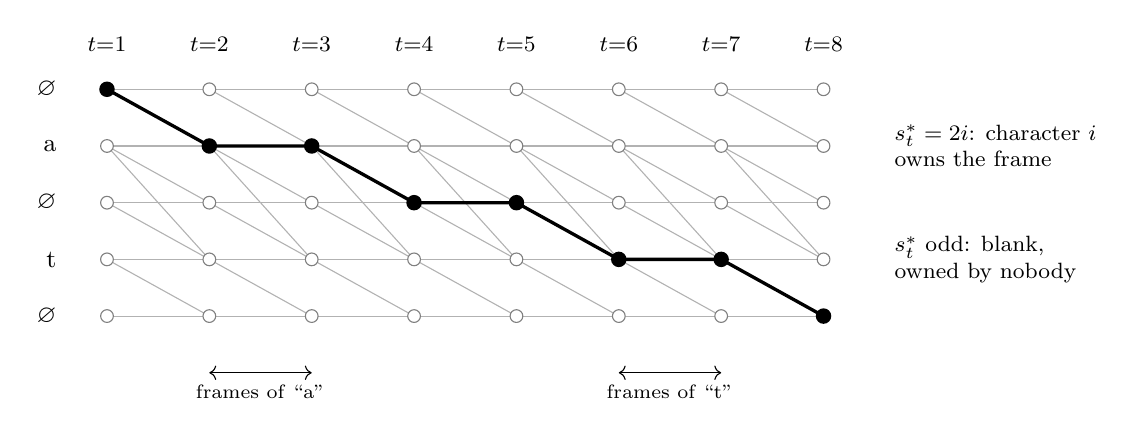
\begin{tikzpicture}[x={(1.3cm,0)},y={(0,-0.72cm)}]
\foreach \t in {1,...,7} {
  \foreach \s in {1,...,5} {\draw[gray!60] (\t,\s) -- (\t+1,\s);}
  \foreach \s in {1,...,4} {\draw[gray!60] (\t,\s) -- (\t+1,\s+1);}
  \draw[gray!60] (\t,2) -- (\t+1,4);
}
\foreach \t in {1,...,8} {\foreach \s in {1,...,5} {\fill[white,draw=gray] (\t,\s) circle (2.3pt);}}
\foreach \s/\l in {1/$\varnothing$,2/a,3/$\varnothing$,4/t,5/$\varnothing$} {\node[font=\small,anchor=east] at (0.6,\s) {\l};}
\foreach \t in {1,...,8} {\node[font=\footnotesize,anchor=south] at (\t,0.5) {$t{=}\t$};}
\draw[very thick] (1,1) -- (2,2) -- (3,2) -- (4,3) -- (5,3) -- (6,4) -- (7,4) -- (8,5);
\foreach \t/\s in {1/1,2/2,3/2,4/3,5/3,6/4,7/4,8/5} {\fill (\t,\s) circle (2.8pt);}
\draw[<->] (2,6.0) -- (3,6.0); \node[font=\scriptsize,anchor=north] at (2.5,6.05) {frames of ``a''};
\draw[<->] (6,6.0) -- (7,6.0); \node[font=\scriptsize,anchor=north] at (6.5,6.05) {frames of ``t''};
\node[font=\footnotesize,anchor=west,align=left] at (8.6,2) {$s^*_t=2i$: character $i$\\ owns the frame};
\node[font=\footnotesize,anchor=west,align=left] at (8.6,4) {$s^*_t$ odd: blank,\\ owned by nobody};
\end{tikzpicture}
\caption{Forced-alignment lattice for the transcript ``at'' with $T=8$ steps (cf.\ Figure~\ref{fig:rec-ctc}). The thick path is the Viterbi path of Equation~\ref{eq:sty-viterbi}; only the frames on the row of a letter belong to that letter, so the spans are narrow.}
\label{fig:sty-lattice}
\end{figure}

\paragraph{Frame-to-pixel conversion and line selection.}
Because the recogniser input is left-aligned with the uniform scale of Equation~\ref{eq:rec-resize}, a frame boundary converts exactly back to a pixel position in the crop: by Equation~\ref{eq:sty-f2p} the frame boundary $a$ lies at the original pixel
\begin{equation}
x_{\mathrm{px}}(a)=\frac{640\,a}{T\,s},\qquad s=\min\Bigl(\frac{64}{h},\frac{640}{w}\Bigr),
\label{eq:sty-f2p}
\end{equation}
for a crop of $h\times w$ pixels, so Equation~\ref{eq:sty-f2p} gives about 6 pixels per frame for a 980-pixel line.
The \emph{alignment confidence} is the mean log-probability along the path, Equation~\ref{eq:sty-conf},
\begin{equation}
\mathrm{conf}=\frac1T\sum_{t=1}^{T}\ell_t\bigl(y'_{s^*_t}\bigr),
\label{eq:sty-conf}
\end{equation}
and the value of Equation~\ref{eq:sty-conf} is low if the recogniser never really read the line, so every line below the 25th percentile of the writer's own confidences is dropped, provided at least eight lines exist: 22 of the 88 lines of writer 153 are discarded in this way.

\paragraph{Cutting the ink into territories.}
CTC spans are narrow slivers that lag the ink, so only their centres $c_k$ (pixels, Equation~\ref{eq:sty-f2p}) are used, with the provisional boundary $\hat x_k=\tfrac12(c_{k-1}+c_k)$ between two characters.
In cursive the only honest boundary is a ligature, where the ink is thin and low, so the boundary is snapped by Equation~\ref{eq:sty-cut} to
\begin{equation}
\begin{aligned}
\mathrm{cost}(x)&=\mathrm{thin}(x)+1.15\,\mathrm{top}(x),\qquad r=\max\bigl(3,\mathrm{round}(0.5x_h)\bigr),\\
x^*&=\arg\min_{|x-\hat x_k|\le r}\Bigl[\mathrm{cost}(x)+0.6\,\frac{|x-\hat x_k|}{r}\Bigr],
\end{aligned}
\label{eq:sty-cut}
\end{equation}
where in Equation~\ref{eq:sty-cut} $\mathrm{thin}(x)$ is the smoothed column ink count divided by its 60th percentile over non-empty columns, $\mathrm{top}(x)$ the height of the highest ink above the baseline in x-heights (limited to 3), the cost is zero in empty columns, and $x_h$ is the x-height of Equation~\ref{eq:wid-xh}.
The cuts are vertical: cutting along the slant lowered the writer identification of the synthesised output from 81.8\,\% to 68.6\,\% (shape classifier, design-stage measurement without raw log), because vertically cut glyphs retile more naturally.

\subsubsection{From ink to ordered pen paths}

\paragraph{Binarisation, core band and slant.}
Each line is binarised like the shape classifier's input (Otsu threshold, rule removal by Equation~\ref{eq:wid-rule}, closing and speck removal; Section~\ref{sec:wid-strokenorm}), and the baseline and x-height $x_h$ come from the core band of Equation~\ref{eq:wid-xh}, whose median over the thirteen writers ranges from 15 to 47 pixels.
The \emph{slant} is the shear that makes the strokes vertical, and it is estimated by the sheared vertical-projection method of Vinciarelli and Luettin~\cite{vinciarelli2001} \mustdo{confirm the page range of the Vinciarelli and Luettin reference (Pattern Recognition Letters, vol.~22, no.~9) in the bibliography; it was left out rather than guessed.}.
For ink pixels $(x_i,y_i)$ with mean row $\bar y$ and trial angle $\theta$ (image $y$ downwards), Equation~\ref{eq:sty-slant} defines the sheared column histogram and its score,
\begin{equation}
x'_i(\theta)=\bigl\lfloor x_i-(y_i-\bar y)\tan\theta\bigr\rfloor,\qquad H_\theta(c)=\#\{i:x'_i(\theta)=c\},\qquad S(\theta)=\sum_cH_\theta(c)^2 ,
\label{eq:sty-slant}
\end{equation}
and $\hat\theta=-\arg\max_\theta S(\theta)$ over $\theta\in\{-45^\circ,-43.5^\circ,\ldots,45^\circ\}$, forward lean positive: since $\sum_cH_\theta(c)$ is fixed, the score of Equation~\ref{eq:sty-slant} peaks when the ink falls in fewest columns.

\paragraph{Thinning and tracing.}
The whole line is thinned \emph{once} with the Zhang--Suen algorithm~\cite{zhang1984} (Equation~\ref{eq:wid-zs}) and only then cut at the territories, because thinning each slice separately creates a spurious spine along the cut.
The skeleton pixels form a graph in the 8-neighbourhood, which is walked into chains: walks start from ends and junctions and follow degree-2 pixels, and chains shorter than 2.5 pixels with a free end are pruned as spurs.
A pen stroke that crosses itself (loops of e, l, o; the bar of t) appears as several chains at a junction, so chain ends within 1.5 pixels of one another are merged repeatedly in order of the smallest continuation angle, the test of Equation~\ref{eq:sty-join},
\begin{equation}
\varphi=\arccos\bigl(-\mathbf d_i\cdot\mathbf d_j\bigr)<75^\circ,
\label{eq:sty-join}
\end{equation}
where $\mathbf d_i,\mathbf d_j$ in Equation~\ref{eq:sty-join} are the outward unit directions of the two ends, so that $\varphi=0$ is a straight continuation.
A chain that crosses a territory boundary is split, and each crossing records that the pen did not lift between the two characters (flags $\mathrm{connL}_i$, $\mathrm{connR}_i$).

\paragraph{Douglas--Peucker simplification.}
Thinning leaves a pixel staircase, so each chain is simplified with the Douglas--Peucker algorithm~\cite{douglas1973}, which recursively splits the chain at the vertex farthest from the chord through its end points $a,b$ until that distance falls below the tolerance $\varepsilon=0.6$ pixels (0.05 to 0.12\,mm at 4\,mm per x-height).
Of a chain with first and last vertex $a,b$, the vertex $p_i$ farthest from the line through $a$ and $b$ has the distance of Equation~\ref{eq:sty-dp},
\begin{equation}
d_i=\frac{\bigl|(b_x-a_x)(p_{i,y}-a_y)-(b_y-a_y)(p_{i,x}-a_x)\bigr|}{\lVert b-a\rVert+10^{-9}},
\label{eq:sty-dp}
\end{equation}
and if $\max_id_i>\varepsilon$ the chain is split there and both halves are simplified recursively, otherwise only $a$ and $b$ are kept; Figure~\ref{fig:sty-dp} sketches the recursion.
\emph{Implementation note:} Equation~\ref{eq:sty-dp} is the distance to the infinite line, not clamped to the segment, so on a closed chain with $a\approx b$ the chord has no length and the whole loop would collapse to two identical points --- which is why the implementation splits closed curves first.
Before the recursion, \texttt{SimplifyPolyline} measures the distance of every vertex from the first, and if the last vertex lies no farther than $\max(1.5,\,0.25\max_i\lVert p_i-p_0\rVert)$ pixels from it the chain is treated as closed, split at its farthest vertex, and the two open halves are simplified separately and rejoined.
The loops of e, l and o are therefore kept.

\begin{figure}[!htbp]
\centering
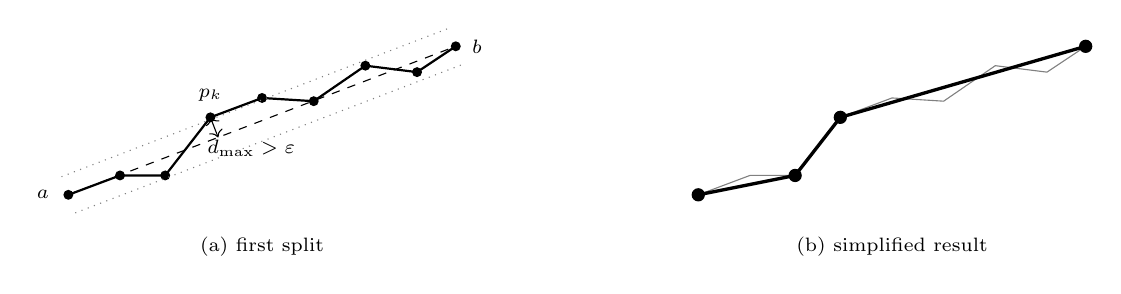
\begin{tikzpicture}[x=0.82cm,y=0.82cm]
\newcommand{\dppoly}[1]{\draw[#1] (0,0) -- (0.8,0.3) -- (1.5,0.3) -- (2.2,1.2) -- (3.0,1.5) -- (3.8,1.45) -- (4.6,2.0) -- (5.4,1.9) -- (6.0,2.3);}
\dppoly{thick}
\foreach \p in {(0,0),(0.8,0.3),(1.5,0.3),(2.2,1.2),(3.0,1.5),(3.8,1.45),(4.6,2.0),(5.4,1.9),(6.0,2.3)} {\fill \p circle (1.8pt);}
\draw[dashed] (0,0) -- (6.0,2.3);
\draw[gray,dotted] (-0.107,0.280) -- (5.893,2.580);
\draw[gray,dotted] (0.107,-0.280) -- (6.107,2.020);
\draw[<->] (2.2,1.2) -- (2.32,0.889);
\node[font=\scriptsize,anchor=west] at (2.0,0.72) {$d_{\max}>\varepsilon$};
\node[font=\scriptsize,anchor=east] at (-0.15,0) {$a$};
\node[font=\scriptsize,anchor=west] at (6.1,2.3) {$b$};
\node[font=\scriptsize] at (2.2,1.55) {$p_k$};
\node[font=\scriptsize,anchor=north] at (3.0,-0.5) {(a) first split};
\begin{scope}[xshift=8.0cm]
\dppoly{gray}
\draw[very thick] (0,0) -- (1.5,0.3) -- (2.2,1.2) -- (6.0,2.3);
\foreach \p in {(0,0),(1.5,0.3),(2.2,1.2),(6.0,2.3)} {\fill \p circle (2.4pt);}
\node[font=\scriptsize,anchor=north] at (3.0,-0.5) {(b) simplified result};
\end{scope}
\end{tikzpicture}
\caption{Douglas--Peucker simplification (schematic, tolerance exaggerated). (a) The vertex $p_k$ with the largest distance $d_{\max}$ from the chord $ab$ lies outside the tolerance band (dotted) and splits the chain. (b) After recursion on both halves four of the original nine vertices remain.}
\label{fig:sty-dp}
\end{figure}

\paragraph{Normalisation and resampling.}
Every simplified point $(x,y)$ (pixels, $y$ down) of a chain in the territory $[L,R)$ goes, by Equation~\ref{eq:sty-norm}, to the writer-independent frame with baseline 0, $y$ up, unit x-height and the slant removed:
\begin{equation}
y_n=\frac{y_b-y}{x_h},\qquad x_n=\frac{x-L}{x_h}-\sigma\,y_n,\qquad\sigma=\tan\hat\theta .
\label{eq:sty-norm}
\end{equation}
The synthesiser applies the inverse shear (Equation~\ref{eq:syn-place}) to the result of Equation~\ref{eq:sty-norm}, so glyphs are stored upright and re-appear at the writer's lean.
A cursive cut falls inside a ligature, so on a side confirmed connected the outward-running low connector is trimmed, and only if at least 18\,\% of the glyph width remains; the entry and exit points are recorded for the synthesiser's own connector.
Kept variants are then resampled at 0.055 x-heights of arc length and smoothed with two passes of the binomial filter of Equation~\ref{eq:sty-smooth} (end points fixed),
\begin{equation}
q_i\leftarrow\tfrac14q_{i-1}+\tfrac12q_i+\tfrac14q_{i+1}
\label{eq:sty-smooth}
\end{equation}
because without the smoothing of Equation~\ref{eq:sty-smooth} the pixel staircase left by thinning (median turn angle $8.9^\circ$, 90th percentile $59.5^\circ$) would be drawn as hand tremor.

\subsubsection{Variants, quality gates and the cross-writer letter prior}

Of about 2\,122 to 4\,031 raw instances per writer roughly 10\,\% survive five gates, applied per character in order:
(1) \emph{geometry} (size limits, at most six strokes, a class prior on height, no swallowed neighbour, and a pen length above an \emph{adaptive} floor);
(2) \emph{outliers} (width and height within fixed ratios of the 40th-percentile width and the median height);
(3) the \emph{cross-writer prior} of Equation~\ref{eq:sty-prior}, which keeps the 70\,\% nearest;
(4) \emph{consensus}: the nearest 75\,\% to the L1-medoid of the kept descriptors are kept, removing glyphs contaminated by a neighbour;
(5) \emph{typicality}: the best 12 by closeness to the reference width and height are kept.
The pen-length floor of gate~(1) is not a fixed number of x-heights: the live gate is $\max(\texttt{MIN\_PEN\_ABS},\ \texttt{FRAGMENT\_PEN\_FRAC}\cdot\tilde p_c)$ with $\texttt{FRAGMENT\_PEN\_FRAC}=0.5$, $\texttt{MIN\_PEN\_ABS}=0.30$ x-heights and $\tilde p_c$ the median pen length of that character's own instances, because a dotless i is much shorter than an o and a single fixed floor either kept neighbour bleed or discarded real short letters.
(An earlier fixed floor of 1.05 x-heights survives only in the retired tree and is not the gate of the delivered builder.)
\emph{Cross-writer prior.} One writer's ten pages cannot show what a clean letter is; thirteen writers can. A glyph becomes a shape descriptor $v_g$ (points along its strokes accumulated on a $12\times12$ grid over its bounding box, damped, blurred and normalised to unit length); the prior $\bar v_c$ of a character is the normalised element-wise median over all writers, and a glyph's distance is given by Equation~\ref{eq:sty-prior},
\begin{equation}
\mathrm{priorD}(g,c)=1-v_g\cdot\bar v_c\in[0,1].
\label{eq:sty-prior}
\end{equation}
The 70\,\% nearest by Equation~\ref{eq:sty-prior} are kept; the prior only \emph{rejects} malformed variants and later gates substitution, and never imports another writer's shapes.
Two derived glyphs are also stored: the \emph{medoid}, the real variant closest to all others (the writer's own ``ideal'' letter), and a \emph{denoised prototype}, the per-stroke median curve of the modal stroke-count group, which is prepended (so a library can hold 13 variants) only if it is clearly cleaner than the variants it summarises.
Figure~\ref{fig:sty-glyphs} shows stored variants.

\begin{figure}[!htbp]
\centering

\includegraphics[width=\linewidth]{Figures/w3_glyphs153_ae.png}
\caption{Stored variants of the letters a, b, c, d and e of writer 153 (a strongly joined hand) in the glyph grid of the web interface; each row is one character with up to 12 variants. The short tails at the sides are remains of ligatures.}
\label{fig:sty-glyphs}
\end{figure}

\subsubsection{Style statistics and permanent storage}

Besides glyphs the profile holds numbers measured over the kept lines (Table~\ref{tab:sty-schema} lists every key of a style-profile file with its meaning and an example value from the profile of writer 153): slant, x-height, stroke width, typical ascender and descender reach, the median advance of each character, the word gap, and the \emph{connectedness} of Equation~\ref{eq:sty-conn},
\begin{equation}
c=\frac{\#\{\text{adjacent letter pairs with }\mathrm{connR}\}}{\#\{\text{adjacent letter pairs}\}}.
\label{eq:sty-conn}
\end{equation}
The numerator of Equation~\ref{eq:sty-conn} counts the pen-down crossings recorded during tracing.
The word gap is measured on the \emph{real} ink (median of ink-free column runs wider than $0.5x_h$), because CTC gives a space only a narrow slice, and the slant and reach of the real lines are stored for the calibration of Section~\ref{sec:syn-cal}.

{
\fontsize{9.5}{11.5}\selectfont
\setlength{\tabcolsep}{4pt}
\begin{longtable}{|p{3.2cm}|p{1.6cm}|p{6.6cm}|p{2.5cm}|}
\hline
\textbf{Key} & \textbf{Type} & \textbf{Meaning} & \textbf{Example (153)} \\
\hline
\endfirsthead
\hline
\textbf{Key} & \textbf{Type} & \textbf{Meaning} & \textbf{Example (153)} \\
\hline
\endhead
\hline
\endfoot
\texttt{authorId} & string & Writer identifier. & \texttt{"153"} \\
\hline
\texttt{slantDeg} & float & Median slant of the lines, forward lean positive (Equation~\ref{eq:sty-slant}). & 30.0 \\
\hline
\texttt{xHeightPx} & float & Median pixel x-height of the kept lines. & 33.0 \\
\hline
\texttt{strokeWidthXh} & float & Ink area divided by skeleton length, in x-heights. & 0.189 \\
\hline
\texttt{ascender}, \texttt{descender} & float & Typical reach of tall and descending lower-case glyphs, in x-heights (defaults 1.7 and $-0.6$ if no glyph qualifies). & 1.59, $-1.10$ \\
\hline
\texttt{wordSpaceXh} & float & Word gap measured on the real ink, in x-heights. & 1.59 \\
\hline
\texttt{connectedness} & float & Fraction of adjacent in-word letter pairs that the pen joins (Equation~\ref{eq:sty-conn}). & 0.961 \\
\hline
\texttt{letterAdvance} & dict & Median advance of each character, in x-heights (45 keys). & \texttt{T}: 1.438, \texttt{e}: 1.147 \\
\hline
\texttt{nLines} & int & Number of lines that survived the alignment-confidence cut. & 66 \\
\hline
\texttt{slantMeasRef}, \texttt{ascMeasRef}, \texttt{descMeasRef} & float & Slant (degrees) and ascender and descender reach of the real full lines, measured with the estimators later used on synthesised renders; input of the style calibration (Equation~\ref{eq:syn-cal}). & 30.0, 1.933, $-1.468$ \\
\hline
\texttt{inkFracRef}, \texttt{aspectRef}, \texttt{paperLevel}, \texttt{inkLevel}, \texttt{midFracRef} & float & Ink fraction, width-to-height ratio and grey statistics of the real lines; stored but ignored while the constant pen width is used for rendering. & 0.0620, 14.95, 246, 81, 0.038 \\
\hline
\texttt{glyphs} & dict & Variant library: for each character a list of at most 13 variant dictionaries (37 characters and 283 variants for writer 153). & see below \\
\hline
\texttt{idealGlyphs} & dict & Per-stroke median prototype of a letter (23 characters), with the keys \texttt{strokes}, \texttt{priorD}, \texttt{advance}, \texttt{lead}, \texttt{width}, \texttt{top}, \texttt{bot}, \texttt{entryY}, \texttt{exitY}, \texttt{nPool}. & --- \\
\hline
\texttt{idealMedoid} & dict & The real variant that is most typical of the writer (29 characters), same keys; this is the anchor used by the synthesiser. & --- \\
\hline
\texttt{legibilityLambda} & float & Legibility parameter $\lambda$ of Equations~\ref{eq:syn-global} and~\ref{eq:syn-swap}; written by the tuner after the build, \emph{not} by the builder. \textbf{Absent from all thirteen stored profiles}, so the deployed code falls back to $\lambda=0$ (see below). & not present \\
\hline
\multicolumn{4}{|l|}{\textbf{Keys of one variant in \texttt{glyphs[c][i]}}} \\
\hline
\texttt{char} & string & The character. & \texttt{"e"} \\
\hline
\texttt{strokes} & list & Strokes, each a list of $[x,y]$ points in x-height units, baseline $y=0$, upright. & 2 strokes, 4 and 33 points \\
\hline
\texttt{width}, \texttt{advance}, \texttt{lead} & float & Ink width, cell width and gap before the ink, in x-heights. & 0.903, 1.097, 0.0 \\
\hline
\texttt{top}, \texttt{bot} & float & Highest and lowest point. & 0.871, 0.0 \\
\hline
\texttt{entryX}, \texttt{entryY}, \texttt{exitX}, \texttt{exitY} & float & Entry and exit points of the pen for connectors. & $-0.149$, 0.258, 0.847, 0.097 \\
\hline
\texttt{connL}, \texttt{connR} & bool & The pen was joined to the left or right neighbour. & true, true \\
\hline
\texttt{priorD} & float & Cosine distance to the cross-writer letter prior (Equation~\ref{eq:sty-prior}). & 0.1179 \\
\hline
\texttt{denoised} & bool & Present and true if the variant is the denoised prototype. & --- \\
\hline
\caption{Keys of a style-profile file (JavaScript Object Notation). The example column was re-read from the stored file \texttt{StyleProfiles10/153.json}; an earlier version of this table quoted the values of a superseded build of that profile.}
\label{tab:sty-schema}
\end{longtable}
}

The thirteen writers differ widely (Table~\ref{tab:sty-writers}, which lists the scalar values of all thirteen stored profiles, re-read from the files themselves): slant from $-10.5^\circ$ to $42.0^\circ$, connectedness 0.195 to 0.968, word gap 0.94 to 2.68 x-heights, the diversity requirement R1 asks the system to reproduce.

\begin{table}[!htbp]
\centering
\fontsize{9}{11}\selectfont
\setlength{\tabcolsep}{3pt}
\begin{tabular}{|l|r|r|r|r|r|r|r|r|r|r|r|}
\hline
\textbf{Writer} & \textbf{Lines} & \textbf{Slant ($^\circ$)} & \textbf{$x_h$ (px)} & \textbf{Stroke width} & \textbf{$A$} & \textbf{$D$} & \textbf{Gap} & \textbf{Conn.} & \textbf{$\lambda$} & \textbf{Chars} & \textbf{Var.} \\
\hline
150 & 61 & $-4.5$ & 47 & 0.096 & 1.58 & $-0.72$ & 1.33 & 0.343 & 0.90$^\dagger$ & 42 & 296 \\
151 & 58 & 33.0 & 22 & 0.271 & 2.69 & $-1.09$ & 1.59 & 0.968 & 1.00$^\dagger$ & 43 & 287 \\
152 & 59 & 19.5 & 46 & 0.104 & 1.48 & $-0.79$ & 1.47 & 0.715 & 0.45$^\dagger$ & 38 & 273 \\
153 & 66 & 30.0 & 33 & 0.189 & 1.59 & $-1.10$ & 1.59 & 0.961 & 0.45$^\dagger$ & 37 & 283 \\
384 & 54 & 4.5 & 43 & 0.107 & 1.93 & $-0.71$ & 1.37 & 0.500 & 0.30$^\dagger$ & 36 & 252 \\
551 & 58 & 42.0 & 20 & 0.225 & 1.84 & $-0.67$ & 2.68 & 0.557 & 1.00$^\dagger$ & 38 & 271 \\
552 & 47 & $-10.5$ & 32 & 0.148 & 1.62 & $-0.56$ & 1.53 & 0.609 & 0.00$^\dagger$ & 40 & 288 \\
588 & 58 & 0.0 & 29 & 0.163 & 1.73 & $-0.68$ & 2.07 & 0.668 & 0.30$^\dagger$ & 41 & 254 \\
abhinav & 130 & 6.0 & 28 & 0.141 & 1.78 & $-0.84$ & 2.13 & 0.789 & --- & 56 & 335 \\
dylan & 79 & $-6.0$ & 26 & 0.135 & 1.68 & $-0.62$ & 1.79 & 0.195 & 1.00$^\dagger$ & 42 & 302 \\
owen & 93 & 0.0 & 32 & 0.111 & 1.51 & $-0.68$ & 1.10 & 0.319 & --- & 43 & 307 \\
thiya & 48 & 30.75 & 15 & 0.331 & 2.24 & $-1.00$ & 1.65 & 0.962 & --- & 42 & 239 \\
yeukita & 74 & 0.0 & 27 & 0.151 & 1.45 & $-0.58$ & 0.94 & 0.417 & 0.15$^\dagger$ & 58 & 333 \\
\hline
\end{tabular}
\caption{Scalar values of the thirteen stored style profiles, read directly from the files in \texttt{Software/CNN/NOGIT/StyleProfiles10}: kept lines, slant, pixel x-height, stroke width (x-heights), ascender $A$ and descender $D$ and word gap (x-heights), connectedness, legibility parameter $\lambda$, number of characters and number of variants. Writers 150 to 588 are database writers, the last five are the personal writers. $^\dagger$The $\lambda$ column is \emph{not} read from these files: the key \texttt{legibilityLambda} is absent from every one of them, and the values shown are the output of an earlier tuning run that predates the current profiles; abhinav, owen and thiya were added afterwards and were never tuned. An earlier version of this table listed ten writers and the scalar values of a superseded build.}
\label{tab:sty-writers}
\end{table}

\paragraph{The legibility parameter is not in the stored profiles.}
The legibility parameter $\lambda$ (Section~\ref{sec:synthesis}) is written into the file after the build by the tuner \texttt{TuneLegibility} of \texttt{Evaluate.py}, not by the builder, and \emph{the key is absent from all thirteen files as delivered}: the profiles were rebuilt after the tuner last ran and the tuner was not re-run on them.
Every reader of the key in the synthesiser supplies a default when it is missing, and the default on the deployed path is zero --- the server calls \texttt{SynthesizeJointBestOf}, which takes \texttt{profile.get('legibilityLambda',\,0.0)} --- so \emph{the delivered system synthesises every writer at $\lambda=0$}, that is, entirely from the writer's own glyphs with no legibility anchor substitution at all.
(One older entry point, \texttt{SynthesizeLegible}, falls back to \texttt{DEFAULT\_LEGIBILITY}${}=0.65$ instead, but the server does not use it.)
The $\lambda$ values of Table~\ref{tab:sty-writers} are genuine measurements of the tuning run that produced them and are retained for that reason, but they describe neither the stored profiles nor the behaviour of the delivered system, and the design-stage gains attributed to per-writer $\lambda$ in Section~\ref{sec:synthesis} are therefore not realised by the code as submitted.
\mustdo{re-run \texttt{TuneLegibility} over the thirteen current profiles so that \texttt{legibilityLambda} is written back into each file, then re-measure the figures of Table~\ref{tab:syn-evid} that depend on it; until this is done the per-writer legibility control described in Section~\ref{sec:synthesis} is inactive.}

\emph{Permanent storage (R6):} a profile is a JavaScript Object Notation (JSON) text file of 290 to 497\,kB (about 4.8\,MB for all thirteen), loaded when the server starts (Section~\ref{sec:system}); thirteen profiles exist and the web interface lists them.
\mustdo{the demonstration of R6 (display of the stored writers, reproduction in a writer chosen by the examiner) and the storage device holding the files.}

\subsubsection{Design alternatives and justification}

Table~\ref{tab:sty-alt} lists the alternatives with the reason for the chosen design.
Fixed widths, projection minima or hand labelling would replace the forced alignment, but joined letters have no gaps, hand labelling of about 90 pages is impractical, and the recogniser already knows the text.
One averaged letter per writer blurs letters whose strokes are arranged differently, whereas variants keep the natural variation; importing the median shape into every writer would erase the writer, whereas filtering keeps the shapes the writer's own; and a generator learned from on-line pen data is impossible, because no such data exist for the thirteen writers (47 to 130 usable lines each).
Cutting a joined line destroys how a letter changes with its neighbours, so the most joined hands (writers 151 and 551) are reproduced least legibly (Section~\ref{sec:synthesis}).

\begin{table}[!htbp]
\centering
\fontsize{9.5}{11.5}\selectfont
\begin{tabularx}{\linewidth}{|p{3.0cm}|X|X|}
\hline
\textbf{Decision} & \textbf{Alternative} & \textbf{Reason for the chosen design} \\
\hline
Character boundaries & Fixed widths, projection minima, hand labelling. & Joined letters have no gaps and hand labelling of about 90 pages is impractical; the recogniser knows the text, so alignment is automatic. \\
\hline
Thin whole line, then cut & Thin each slice. & A slice edge creates a spurious spine stored as a bar. \\
\hline
Several variants per letter & One averaged letter. & Averaging blurs letters whose strokes are arranged differently; variants keep the natural variation, medoid and prototype remain options. \\
\hline
Prior as a filter & Import the median shape into every writer. & Importing would erase the writer; filtering keeps the shapes the writer's own. \\
\hline
Glyphs from scanned pages & Generator learned from on-line pen data. & No on-line data of the thirteen writers exist (47 to 130 usable lines each), and the pen path must be recovered from the image in any case (Section~\ref{sec:synthesis}). \\
\hline
\end{tabularx}
\caption{Design alternatives for the style extraction.}
\label{tab:sty-alt}
\end{table}

A real example of the builder stages, Figure~\ref{fig:sty-stages}, is still to be supplied.

\begin{figure}[!htbp]
\centering
\figplaceholder{3.4cm}{One real line of a database writer and one personal line: grey crop, ink mask with rules removed and core band, Zhang--Suen skeleton, traced chains in colours with the territory cuts as vertical lines, and one extracted glyph in the normalised frame. Source: the functions of the profile builder applied to a crop of \texttt{Data/Datasets/IAMpages10} and one of \texttt{Software/CNN/NOGIT/dylan}.}
\caption{Stages of the style builder on real lines (placeholder).}
\label{fig:sty-stages}
\end{figure}


\subsection{Handwriting synthesis}
\label{sec:synthesis}

This subsection describes how a text is converted into pen paths in the style of a stored writer (functional units FU~2.7 and part of FU~2.5; requirements R1 and R3).
The synthesiser takes the text, a style profile (Section~\ref{sec:styleprofile}), the x-height size $x_{\mathrm{mm}}$ in millimetres (4\,mm by default) and a random seed, and returns a \emph{trajectory}: pen-down polylines in millimetres, $y$ upwards, origin at the first baseline.
The construction is random, so a search over several candidates (Section~\ref{sec:syn-search}) keeps the one that the text recogniser (Section~\ref{sec:textrec}) and the stroke-normalised writer classifier (Section~\ref{sec:writerid}) jointly prefer.
Geometry stays in x-height units until one multiplication at the end, so one profile serves any pen size.

\subsubsection{Global quantities and glyph choice}

Let $\theta_{\mathrm p}$ be the slant, $c$ the connectedness, $A$ and $D<0$ the ascender and descender reach and $g$ the word gap of the profile, and $\lambda\in[0,1]$ the writer's legibility parameter (below; in the delivered system $\lambda=0$ for every writer, because the key is missing from the stored profiles --- Section~\ref{sec:styleprofile}, so every formula below that contains $\lambda$ should be read at $\lambda=0$ when judging what the submitted code does).
The synthesiser derives, in Equation~\ref{eq:syn-global},
\begin{equation}
\theta_{\mathrm{cap}}=45^\circ-19^\circ\lambda,\quad\sigma=\tan\!\bigl(\operatorname{clip}(\theta_{\mathrm p},\pm\theta_{\mathrm{cap}})\bigr)+\Delta_\sigma,\quad p_{\mathrm j}=\min(c,1),\quad L=(A-D+0.85)\,x_{\mathrm{mm}},
\label{eq:syn-global}
\end{equation}
the shear coefficient $\sigma$ (calibration shift $\Delta_\sigma$, Section~\ref{sec:syn-cal}), the join probability $p_{\mathrm j}$ and the line pitch $L$, which Equation~\ref{eq:syn-global} puts at 12.6\,mm for $A=1.7$, $D=-0.6$ and $x_{\mathrm{mm}}=4$\,mm.
The connectedness is a \emph{probability}: as a threshold it joined every pair for every writer above it and fused words into blobs.

For each character the synthesiser tries, in order, the writer's own variants, a borrowed shape (other case or similar character), the \emph{anchor} glyph, and finally a hand-designed skeleton or a blank.
Variants are ranked by $\mathrm{priorD}$ (Equation~\ref{eq:sty-prior}); only the five best are eligible, and rank $i=0,\ldots,4$ is drawn with probability proportional to the weight of Equation~\ref{eq:syn-pick},
\begin{equation}
w_i=\frac{1}{1+1.4\,i}\exp\!\Bigl[-\Bigl(\frac{\mathrm{entryY}_i-\hat e}{0.45}\Bigr)^2\Bigr],
\label{eq:syn-pick}
\end{equation}
where the exponential factor of Equation~\ref{eq:syn-pick} applies only when the glyph is joined to a previous letter and $\hat e$ is the pen's exit height above the baseline in x-heights: a variant whose entry height matches the pen avoids tangled joins.
Without that exponential factor the five eligible ranks are drawn with probabilities $0.494$, $0.206$, $0.130$, $0.095$ and $0.075$.
A writer forms a letter consistently, and restricting the choice to typical variants gave 80.5\,\% writer identification with the two best variants against 75.5\,\% over all twelve (design-stage measurement, no raw log).

\paragraph{The anchor glyph.}
The \emph{anchor} is a legible stand-in: it is the writer's own medoid if that medoid has $\mathrm{priorD}\le0.30$, and otherwise a hand-designed single-stroke skeleton, joined cursive for $c\ge0.5$ and upright print otherwise, re-proportioned to the writer's reach by $y\mapsto1+(y-1)\max\bigl(0.35,(A-1)/0.75\bigr)$ for $y>1$ and $y\mapsto y\max\bigl(0.35,|D|/0.55\bigr)$ for $y<0$.
The print skeleton reads back at about 96\,\% character and about 84\,\% word accuracy through the recogniser (the figures of the code comment at \texttt{SynthesizeHandwriting.py} line~238, no raw log), which is far clearer than any data-driven consensus glyph, so it is the legibility floor.
\mustdo{the corresponding read-back accuracy of the \emph{cursive} skeleton. An earlier draft of this paragraph quoted about 89\,\% for it; that figure matches no comment or log in the delivered code and has been withdrawn rather than left standing as a measurement.}

\paragraph{The role of $\lambda$.}
The parameter does \emph{not} interpolate geometrically between the writer's glyph and the anchor; it scales the probability, given by Equation~\ref{eq:syn-swap}, that a chosen variant with prior distance $d$ is \emph{replaced} by the anchor,
\begin{equation}
P_{\mathrm{swap}}(\lambda,d)=\begin{cases}1&d\ge0.55,\\0&\lambda\le10^{-3},\\0.06\,\lambda&d\le0.12,\\\operatorname{clip}\bigl(\lambda\,(0.55+0.9\,b),0,1\bigr),\ b=\operatorname{clip}\bigl(\tfrac{d-0.12}{0.43},0,1\bigr)&\text{otherwise,}\end{cases}
\label{eq:syn-swap}
\end{equation}
and it lowers the cap on the writer's own slant (Equation~\ref{eq:syn-global}).
By Equation~\ref{eq:syn-swap} clean glyphs are almost always kept, garbage is always replaced, and in between replacement grows with $\lambda$ (at $\lambda=1$: 0.74 for $d=0.21$, 0.99 for $d=0.33$), so the sources are mixed probabilistically: with the $\lambda$ values of the tuning run the share of anchor glyphs in a design-stage probe ranged from 0\,\% (writer 552, $\lambda=0$) to 76\,\% (writer 151, $\lambda=1$).
$\lambda$ is set per writer (Table~\ref{tab:sty-writers}) by an automatic search on a novel corpus followed by manual adjustment against the evaluation script, so it is tuned on the sentences of Section~\ref{sec:results}.

\emph{Implementation note: in the system as submitted this mechanism is inert.}
The key \texttt{legibilityLambda} is absent from all thirteen stored style profiles, and the entry point the server uses, \texttt{SynthesizeJointBestOf}, defaults the parameter to zero when the key is missing, so $\lambda=0$ for every writer on the live path (Section~\ref{sec:styleprofile}).
The second branch of Equation~\ref{eq:syn-swap} then fires for every glyph whose prior distance is below 0.55, so the \emph{only} anchor substitutions that still happen are the unconditional ones at $d\ge0.55$, and the slant cap of Equation~\ref{eq:syn-global} sits at its widest value $\theta_{\mathrm{cap}}=45^\circ$.
The 0\,\% to 76\,\% range of anchor shares quoted above is therefore the behaviour of the tuned configuration and \emph{not} of the delivered one, where the share is whatever the $d\ge0.55$ rule alone produces; the 76\,\% figure for writer 151 in particular depended on $\lambda=1$ and does not describe the current build.
The $\lambda$ values of Table~\ref{tab:sty-writers} are real measurements of that earlier tuning run and are kept for that reason, labelled as such, and the outstanding item of Section~\ref{sec:styleprofile} to re-run the tuner applies to every $\lambda$-dependent statement in this subsection.
\emph{Further note:} a geometric blend toward the anchor and a ``soft archetype'' proposal appear only in the project notes, not in the delivered code.

\subsubsection{Placement, joins and randomness}

A chosen glyph $(x,y)$ (x-height units, upright) is placed at the pen position $(P_x,P_y)$ (mm) by Equation~\ref{eq:syn-place},
\begin{equation}
X=P_x+(\ell+x+\sigma_g\,y)\,x_{\mathrm{mm}},\qquad Y=P_y+(y+\delta_g)\,x_{\mathrm{mm}},
\label{eq:syn-place}
\end{equation}
with the glyph's lead $\ell$, shear $\sigma_g$ and baseline drift $\delta_g$; Equation~\ref{eq:syn-place} inverts the de-slanting of Equation~\ref{eq:sty-norm}, and Figure~\ref{fig:syn-layout} shows the resulting line-layout geometry.
The writer's own glyphs use $\sigma$; anchor glyphs are limited to $\pm\tan30^\circ$ (cursive) or $\pm\tan22^\circ$ (print), because a $40^\circ$ shear makes even a clean letter collide.
A guard shifts glyph and pen right if the glyph would come closer than $0.05\,x_{\mathrm{mm}}$ to the previous ink, and the pen advances by the glyph's \emph{own} advance, never the character median.
After a word the pen advances by the randomised word gap $g\,x_{\mathrm{mm}}(0.85+0.3u)$ with $u\sim U(0,1)$, and a word that would cross the line width (185\,mm in the server) starts a new line at the pitch $L$.
Adjacent letters are joined if both are alphabetic, both are the writer's own glyphs or both the cursive anchor, and a random $u<p_{\mathrm j}$ (a print anchor is never joined through).
The connector from exit $p_0$ to the next entry $p_1$ is the path of Equation~\ref{eq:syn-lig},
\begin{equation}
\begin{aligned}
&\text{path}(p_0,m,p_1),\qquad m=\Bigl(\tfrac{p_{0x}+p_{1x}}{2},\ \min(p_{0y},p_{1y})-\mathrm{sag}\Bigr),\\
&\mathrm{sag}=\min\bigl(0.11\,x_{\mathrm{mm}},0.16\,|\Delta x|\bigr)+\mathcal N\bigl(0,(0.015\,x_{\mathrm{mm}})^2\bigr),
\end{aligned}
\label{eq:syn-lig}
\end{equation}
with $\Delta x=p_{1x}-p_{0x}$; the sag of Equation~\ref{eq:syn-lig} is proportional to the span because a fixed dip would turn a short join into a loop.
A joined run is one pen-down polyline, so the pen lifts only where the writer lifts, and every polyline is resampled at 0.35\,mm arc length for even plotter motion.
One pseudo-random stream, seeded by the seed argument, supplies every draw, so the arguments fix the output completely.

\begin{figure}[!htbp]
\centering
\begin{tikzpicture}[x=1cm,y=1cm]
\newcommand{\hshape}[1]{\draw[#1] (0.1,0) -- (0.1,1.8); \draw[#1] (0.1,0.6) .. controls (0.3,1.0) and (0.7,1.0) .. (0.75,0.6) -- (0.75,0);}
\draw[gray] (-0.3,0) -- (4.3,0); \node[w3lab,anchor=east] at (-0.3,0) {baseline};
\draw[gray,dashed] (-0.3,1) -- (4.3,1); \node[w3lab,anchor=east] at (-0.3,1) {$y{=}1$};
\begin{scope}[xshift=0.2cm]\hshape{thick}\end{scope}
\begin{scope}[xshift=2.6cm,xslant=0.466]\hshape{thick}\end{scope}
\draw[w3arr] (1.2,0.9) -- (2.2,0.9);
\node[w3lab] at (1.7,1.15) {shear};
\draw[dotted] (2.7,0) -- (2.7,1.8);
\node[font=\scriptsize] at (2.0,-0.45) {(a) $X=\ell+x+y\tan\theta$};
\begin{scope}[xshift=6.3cm]
\draw[gray] (-0.3,0) -- (7.2,0);
\draw[fill=gray!10] (0,0) rectangle (2.3,1.4);
\draw[fill=gray!10] (2.3,0) rectangle (4.3,1.4);
\draw[thick] (0.5,0.1) rectangle (1.9,1.2);
\draw[thick] (2.55,0.1) rectangle (4.0,1.2);
\draw[<->] (0,-0.25) -- (2.3,-0.25); \node[w3lab,anchor=north] at (1.15,-0.25) {advance $a$};
\draw[<->] (0,1.6) -- (0.5,1.6); \node[w3lab,anchor=south] at (0.25,1.6) {$\ell$};
\draw[<->] (1.9,1.6) -- (2.55,1.6); \node[w3lab,anchor=south] at (2.3,1.6) {gap};
\draw[w3arr] (0,-0.9) -- (0.9,-0.9) node[midway,below,w3lab] {$P_x$};
\node[w3lab,anchor=west] at (4.4,0.7) {word gap $g\,x_{\mathrm{mm}}(0.85{+}0.3u)$};
\node[font=\scriptsize] at (3.2,-1.3) {(b) cells, ink boxes and guard};
\end{scope}
\end{tikzpicture}
\caption{Glyph placement. (a) A stored upright glyph is sheared by the writer's slant (Equation~\ref{eq:syn-place}). (b) Each glyph occupies a cell of its own advance $a$; the ink starts after the lead $\ell$, and the collision guard keeps a minimum clear gap between consecutive ink boxes.}
\label{fig:syn-layout}
\end{figure}

\paragraph{Glyph jitter and baseline drift.}
Each glyph receives the random rotation, scaling and translation of amplitude $J$ (0.15 by default, 0.5 in the search) given by Equation~\ref{eq:syn-jit},
\begin{equation}
\begin{pmatrix}x'\\y'\end{pmatrix}=R(\vartheta)\,\mathrm{diag}(s_x,s_y)\begin{pmatrix}x\\y\end{pmatrix}+\begin{pmatrix}d_x\\d_y\end{pmatrix},\quad
\begin{aligned}d_x&\sim\mathcal N(0,(0.022J)^2),&d_y&\sim\mathcal N(0,(0.0132J)^2),\\\vartheta&\sim\mathcal N(0,(2.2^\circ J)^2),&s_{x,y}&\sim1+\mathcal N(0,(0.05J)^2),\end{aligned}
\label{eq:syn-jit}
\end{equation}
with the translations of Equation~\ref{eq:syn-jit} in x-heights; the baseline drifts in addition as a slow first-order walk whose constants are in Table~\ref{tab:syn-const}.
At $J=0.5$ Equation~\ref{eq:syn-jit} gives a translation spread below 0.05\,mm, a rotation of $1.1^\circ$ and a scale change of 2.5\,\%.
Table~\ref{tab:syn-const} collects every remaining constant of the synthesiser and of the jitter model, including those not quoted in the text above.

\begin{table}[!htbp]
\centering
\fontsize{9.5}{11.5}\selectfont
\begin{tabularx}{\linewidth}{|p{5.2cm}|p{2.2cm}|X|}
\hline
\textbf{Constant} & \textbf{Value} & \textbf{Role} \\
\hline
Eligible variants per letter & 5 & Highest-ranked variants that can be drawn (Equation~\ref{eq:syn-pick}). \\
\hline
Clean and garbage prior distances & 0.12 and 0.55 & Limits of Equation~\ref{eq:syn-swap}. \\
\hline
Maximum prior distance of an anchor medoid & 0.30 & Otherwise the generic skeleton is used. \\
\hline
Connected-hand threshold for the cursive anchor & 0.5 & A value above 1 disables the cursive anchor (an earlier configuration used 2.0); lowering it to 0.3 lowered the evaluation score and was reverted. \\
\hline
Slant limit of anchor glyphs & $30^\circ$ / $22^\circ$ & Cursive / print skeleton. \\
\hline
Jitter share of anchor glyphs & 0.15 & Anchor glyphs wobble less. \\
\hline
Collision gap & 0.05 $x_{\mathrm{mm}}$ & Minimum clear space between consecutive ink boxes. \\
\hline
Output resampling and connector step & 0.35\,mm & Arc-length step of every pen-down polyline. \\
\hline
Rendering for the judges & 0.085 $x$, blur 0.30 & Constant pen width in x-heights and Gaussian blur as a fraction of the stroke width; 18 pixels per millimetre; padding $0.18\,x_{\mathrm{mm}}$. \\
\hline
Search stopping scores & 0.99 / 0.995 & Early stop of the candidate loop / no repair above this score. \\
\hline
Repair rounds and pins per round & 3 and 2 & Joint-aware repair pass. \\
\hline
Seed step between candidates & 977 & Candidate $k$ uses $\mathrm{base}+977k$. \\
\hline
Calibration probe & seed 17, $J=0$ & Sentence ``the quick brown fox jumps over lazy dogs and by half past eight it kept flying quietly''. \\
\hline
\end{tabularx}
\begin{tabularx}{\linewidth}{|X|c|c|}
\hline
\textbf{Perturbation (Equation~\ref{eq:syn-jit})} & \textbf{Standard deviation} & \textbf{At $J=0.5$, $x_{\mathrm{mm}}=4$\,mm} \\
\hline
Translation in $x$ / $y$ & $0.022J$ / $0.0132J$ x-heights & 0.044\,mm / 0.026\,mm \\
\hline
Rotation & $2.2^\circ J$ & $1.1^\circ$ \\
\hline
Scale in $x$ and $y$ (independent) & $0.05J$ & 2.5\,\% \\
\hline
Baseline drift (AR(1), clipped) & $0.05J\cdot0.35$ per step, $\pm0.25$ & $\pm0.25$ x-heights \\
\hline
Connector sag noise & $0.015\,x_{\mathrm{mm}}$ & 0.06\,mm \\
\hline
Word-gap factor & uniform 0.85 to 1.15 & --- \\
\hline
\end{tabularx}
\caption{Constants of the synthesiser and the jitter model.}
\label{tab:syn-const}
\end{table}

\paragraph{Style calibration.}
\label{sec:syn-cal}
A line of separate glyphs does not automatically reproduce the line-level slant and reach of the real lines (writer 150's ascenders came out about 7\,\% too tall, writer 551's slant about $9^\circ$ too steep).
A probe sentence is therefore synthesised once per writer and size, measured with the estimators of Section~\ref{sec:styleprofile}, and three fixed-point iterations adjust the shear shift $\Delta_\sigma$ and the scale factors $K_A$, $K_D$ of the writer's own tall and deep strokes until the probe matches the stored real-line values.
Writing ``ref'' for the stored real-line value and ``got'' for the value measured on the probe, the three iterations are those of Equation~\ref{eq:syn-cal},
\begin{equation}
\Delta_\sigma\leftarrow\Delta_\sigma+\tan\theta_{\mathrm{ref}}-\tan\theta_{\mathrm{got}},\quad K_A\leftarrow\operatorname{clip}\Bigl(K_A\frac{A_{\mathrm{ref}}-1}{A_{\mathrm{got}}-1},0.5,1.6\Bigr),\quad K_D\leftarrow\operatorname{clip}\Bigl(K_D\frac{D_{\mathrm{ref}}}{D_{\mathrm{got}}},0.5,1.6\Bigr),
\label{eq:syn-cal}
\end{equation}
in which $\theta$ is the line slant of Equation~\ref{eq:sty-slant}, $A>1$ the ascender reach and $D<0$ the descender reach, the stored reference values being \texttt{slantMeasRef}, \texttt{ascMeasRef} and \texttt{descMeasRef} of Table~\ref{tab:sty-schema}.
The scale factors of Equation~\ref{eq:syn-cal} are applied as $y\leftarrow1+(y-1)K_A$ for $y>1$ and $y\leftarrow yK_D$ for $y<0$ on the writer's own glyphs, the clip to $[0.5,1.6]$ bounding the correction, and $\Delta_\sigma$ is added to the shear coefficient of Equation~\ref{eq:syn-global}.
The probe is synthesised with seed 17 and no jitter (Table~\ref{tab:syn-const}).
The same estimator measures both sides, so the agreement of slant and reach is partly self-fulfilling and not independent evidence.

\subsubsection{Best-of-$N$ search with joint scoring}
\label{sec:syn-search}

Single draws vary in quality, so the line is drawn $N$ times and the best candidate kept.
Selecting by text accuracy alone raised legibility but lowered writer identification for some writers (Table~\ref{tab:syn-evid}): the most legible draw need not be the most characteristic.
The score therefore uses both judges.
For a rendered candidate $I$, with $\hat y(I)$ the greedy CTC reading (Equation~\ref{eq:rec-greedy}) and $y$ the intended text, the joint score is given by Equation~\ref{eq:syn-score},
\begin{equation}
a(I)=\max\Bigl(0,1-\frac{\mathrm{Lev}(\hat y(I),y)}{|y|}\Bigr),\quad w(I)=\mathrm{softmax}\bigl(f_{\mathrm{wid}}(I)\bigr)_{a^\star},\quad S(I)=\frac{2\,a(I)\,w(I)}{a(I)+w(I)},
\label{eq:syn-score}
\end{equation}
where in Equation~\ref{eq:syn-score} $\mathrm{Lev}$ is the Levenshtein distance (Equation~\ref{eq:rec-lev}), $f_{\mathrm{wid}}$ the shape classifier after stroke normalisation (Section~\ref{sec:wid-strokenorm}), $a^\star$ the target writer, and $S=0$ if $a+w\le10^{-9}$.
The harmonic mean is dominated by the smaller term, so a candidate cannot win on one criterion while failing the other, and $w$ is a probability, not a hit-or-miss flag.

\paragraph{Steps of the search and the repair pass.}
The steps of Figure~\ref{fig:syn-flow} are:
(1) for $k=0,\ldots,N-1$, synthesise a candidate with seed $\mathrm{base}+977k$ and $J=0.5$, render it at a constant pen width of 0.085 x-heights (18 pixels per millimetre), compute $S$ (Equation~\ref{eq:syn-score}), keep it if $S>\mathrm{best}$ (initially $-1$), and stop early at $\mathrm{best}\ge0.99$;
(2) \emph{repair} (at most three rounds, skipped if $\mathrm{best}\ge0.995$): forced-align the intended text to the recogniser output on the best image (Equation~\ref{eq:sty-viterbi}) and score each non-space character $i$ by its mean own-class log-probability over its frames, Equation~\ref{eq:syn-weak},
\begin{equation}
m_i=\frac{1}{b_i-a_i}\sum_{t=a_i+1}^{b_i}\ell_t(y_i),
\label{eq:syn-weak}
\end{equation}
where Equation~\ref{eq:syn-weak} is set to $m_i=-10^9$ if the path never visits character $i$, and the characters are sorted ascending by $m_i$;
(3) pin the two worst unpinned characters to the anchor, re-synthesise the \emph{whole} line with seed $\mathrm{base}$, render and score it;
(4) accept only if the joint score strictly exceeds $\mathrm{best}$.
A repaired line is therefore accepted only if the joint score strictly exceeds the best so far, so a repair that fixes a letter but makes the line look like another writer is rejected (a text-only search with a plain repair that accepts on text score alone was measured to cost writer identification; Table~\ref{tab:syn-evid}).

\begin{figure}[!htbp]
\centering
\begin{tikzpicture}[x=1cm,y=1cm]
\tikzset{n/.style={w3box,text width=3.6cm,minimum height=0.7cm,font=\scriptsize},d/.style={w3dec,text width=2.1cm}}
\node[w3io,text width=3.6cm,font=\scriptsize,minimum height=0.7cm] (s0) at (0,0) {Text, writer, $N$, base seed};
\node[n] (s1) at (0,-1.0) {Synthesise candidate $k$, seed $\mathrm{base}+977k$, $J=0.5$};
\node[n] (s2) at (0,-2.0) {Render at constant pen width};
\node[n] (s3) at (0,-3.0) {Judges $a(I)$, $w(I)$; $S(I)$ (Eq.~\ref{eq:syn-score})};
\node[d] (s4) at (0,-4.2) {$S>\mathrm{best}$?};
\node[d] (s5) at (0,-5.7) {$\mathrm{best}\ge0.99$ or $k=N-1$?};
\node[n,text width=2.0cm] (keep) at (3.0,-4.2) {keep candidate};
\node[n] (r1) at (7.0,-0.3) {Forced-align text; rank characters by $m_i$ (Eq.~\ref{eq:syn-weak})};
\node[d] (r0) at (7.0,-1.6) {$\mathrm{best}\ge0.995$ or 3 rounds?};
\node[n] (r2) at (7.0,-2.9) {Pin the 2 worst unpinned characters to the anchor};
\node[n] (r3) at (7.0,-3.9) {Re-synthesise line, seed $=\mathrm{base}$; judge};
\node[d] (r4) at (7.0,-5.0) {$S'>\mathrm{best}$?};
\node[n,text width=2.2cm] (acc) at (10.0,-5.0) {accept; keep pins};
\node[w3io,text width=3.0cm,font=\scriptsize,minimum height=0.7cm] (out) at (7.0,-6.3) {Trajectory to G-code};
\draw[w3arr] (s0) -- (s1); \draw[w3arr] (s1) -- (s2); \draw[w3arr] (s2) -- (s3); \draw[w3arr] (s3) -- (s4);
\draw[w3arr] (s4) -- (keep) node[midway,above,w3lab] {yes};
\draw[w3arr] (s4) -- (s5) node[midway,right,w3lab] {no};
\draw[w3arr] (keep.south) |- (s5.east);
\draw[w3arr] (s5.west) -- ++(-1.6,0) |- (s1.west) node[pos=0.2,left,w3lab] {no};
\draw[w3arr] (s5.south) -- ++(0,-0.45) -| ++(3.6,0) |- (r1.west) node[pos=0.1,right,w3lab] {yes};
\draw[w3arr] (r1) -- (r0);
\draw[w3arr] (r0) -- (r2) node[midway,right,w3lab] {no};
\draw[w3arr] (r2) -- (r3); \draw[w3arr] (r3) -- (r4);
\draw[w3arr] (r4) -- (acc) node[midway,above,w3lab] {yes};
\draw[w3arr] (r4.south) -- (out.north) node[pos=0.3,right,w3lab] {no};
\draw[w3arr] (acc.south) |- (out.east);
\draw[w3arr] (r0.east) -- ++(1.3,0) |- ++(0,-4.4) |- (out.east);
\end{tikzpicture}
\caption{Flow chart of the joint best-of-$N$ search: the search over $N$ candidates (left) and the repair pass (right). A repair round ends after acceptance or rejection and the next round starts from the best candidate; when its test is satisfied the repair loop exits to the output.}
\label{fig:syn-flow}
\end{figure}

If candidate scores were independent with distribution function $F$, then the order statistic of Equation~\ref{eq:syn-order},
\begin{equation}
\Pr\bigl[\max_kS_k\le\tau\bigr]=F(\tau)^N,
\label{eq:syn-order}
\end{equation}
shows that the gain of Equation~\ref{eq:syn-order} grows roughly logarithmically in $N$; the seeds share a profile, so independence is only approximate, and no per-$N$ curve was kept.
\emph{Implementation notes.} (i) The repair re-uses seed $\mathrm{base}$, so it is a fresh draw with pins, not a patch of the winner. (ii) The pin set is updated only on acceptance, so after a rejection the next round re-synthesises an identical candidate and the remaining rounds are wasted work. (iii) In three probe runs (writers 150, 153, 551, $N=14$) no repair was accepted, so the repair pass rarely changes the result.

\paragraph{Values of $N$ and cost.}
$N$ is 6 as the function default, 14 for the design-stage measurements of Table~\ref{tab:syn-evid}, 20 as the web default and 30 in the official evaluation script.
A candidate costs one synthesis, one rendering, one recogniser pass and one classifier pass, so the total cost is that of Equation~\ref{eq:syn-cost},
\begin{equation}
T\approx N\,(T_{\mathrm{syn}}+T_{\mathrm{ren}}+T_{\mathrm{text}}+T_{\mathrm{wid}})+\text{(up to three repair candidates)},
\label{eq:syn-cost}
\end{equation}
and each network pass in Equation~\ref{eq:syn-cost} is about $4\times10^9$ multiply--accumulate operations (Equation~\ref{eq:rec-macs}, Table~\ref{tab:wid-layers}).
Laptop timings per stage are in Table~\ref{tab:syn-cost}: synthesis takes 11 to 16\,ms per candidate and the two judges 0.5 to 4\,s, dominated by thinning the full-resolution render, so the search at $N=14$ took 23 to 137\,s; times on the single-board computer were not recorded.

\begin{table}[!htbp]
\centering
\fontsize{9.5}{11.5}\selectfont
\begin{tabularx}{\linewidth}{|X|c|c|c|}
\hline
\textbf{Quantity (56-character sentence)} & \textbf{Writer 150} & \textbf{Writer 153} & \textbf{Writer 551} \\
\hline
Render size (pixels) & $3585\times225$ & $5508\times207$ & $7876\times277$ \\
\hline
Synthesis of one candidate (ms) & 11 & 13 & 16 \\
\hline
Rendering (ms) & 20 & 27 & 56 \\
\hline
Text recogniser (s) & 0.50 & 0.49 & 0.74 \\
\hline
Writer classifier incl. stroke normalisation (s) & 1.03 & 1.65 & 3.74 \\
\hline
Complete search, $N=14$, with repair attempts (s) & 23 & 37 & 137 \\
\hline
\end{tabularx}
\caption{Indicative cost of the search on the development laptop (single profiling run, unknown background load, jitter 0.5); times on the single-board computer were not recorded.}
\label{tab:syn-cost}
\end{table}

\subsubsection{Design-stage measurements of the synthesiser}

Table~\ref{tab:syn-evid} lists the measurements that motivated the design (six novel sentences, two seeds, ten writers: 12 lines per writer, so one misjudged line moves a writer's rate by 8.3 percentage points), together with the final system for comparison.
\emph{Every figure after the search was introduced is the opinion of the very networks that selected the output}: the search loads the same weight files as the measurement, so a selection effect is added to genuine quality, and $\lambda$, the anchor threshold and $N$ were tuned on the same sentences.
The values show that the pipeline can satisfy these two judges, not that human readers or an independent recogniser agree; the non-circular reference is the recogniser on \emph{real} held-out handwriting of the same writers, 89.4\,\% character and 70.8\,\% word accuracy (Table~\ref{tab:rec-data}; possible training overlap).
Section~\ref{sec:results} reports the final evaluation.

\begin{table}[!htbp]
\centering
\fontsize{9.5}{11.5}\selectfont
\begin{tabularx}{\linewidth}{|X|c|c|}
\hline
\textbf{Stage} & \textbf{Writer ID, direct / G-code (\%)} & \textbf{Char. acc., direct / G-code (\%)} \\
\hline
Plain synthesis after label and glyph fixes & 79.2 / 80.0 & 75.9 / 76.3 \\
\hline
+ per-writer $\lambda$ & 83.3 / 86.7 & 77.2 / 77.8 \\
\hline
Text-only best-of-$N$ with plain repair & 76.7 / 73.3 & 83.8 / 82.7 \\
\hline
Joint best-of-$N$, $N=6$ & 92.5 / 92.5 & 79.9 / 79.6 \\
\hline
Joint best-of-$N$, $N=14$ & 97.5 / 95.8 & 81.6 / 81.4 \\
\hline
\textbf{Final system, 13 writers, 3 sentences, $N=8$} & \textbf{92.3 / 89.7} & \textbf{79.2 / 79.2} \\
\hline
\textbf{Final system, 13 writers, 6 sentences $\times$ 2 seeds, $N=30$} & \textbf{80.1 / 78.8} & \textbf{82.2 / 82.5} \\
\hline
\textbf{Matching comparison: the writers' own handwriting of the same words} & not applicable & \textbf{89.0 / ---} \\
\hline
\textbf{Matching comparison: the system's synthesis of those same words} & not applicable & \textbf{81.6 / ---} \\
\hline
\end{tabularx}
\caption{Measurements that motivated the design (upper rows) and the final system (lower rows). ``G-code'' means converted to G-code and read back (Section~\ref{sec:gcode}). The upper rows and the writer-identification columns are judged by the networks that drive the search and were tuned on the same sentences, so they are not independent evidence; the two matching-comparison rows are independent of the search and are the figures to trust. The gain shown in the ``per-writer $\lambda$'' row is not available in the delivered system: the key \texttt{legibilityLambda} is absent from the stored profiles, so the live path runs at $\lambda=0$ (Section~\ref{sec:styleprofile}).}
\label{tab:syn-evid}
\end{table}

Four remarks follow from Table~\ref{tab:syn-evid}.
First, on the matching comparison of identical words the writers' own hands are read at 89.0\,\% and the synthesis of those words at 81.6\,\% character accuracy, so synthesis costs 7.4 percentage points.
Second, the same comparison divides word accuracy by more than 1.5 (70.5\,\% against 46.7\,\%), locating the loss in spacing and word boundaries rather than letterforms.
Third, at the final settings the two most joined writers stay well below the 85\,\% target: writers 151 and 552 reach 53\,\% and 56\,\% character accuracy through G-code, against about 84\,\% for the other eleven.
This is the clearest limitation of the exemplar approach on strongly cursive hands.
Fourth, the writer-identification figures on synthesised text (80.1\,\% in the official run and 89.7\,\% in the coverage run) come from a classifier that also selects the candidates, so a best-of-$N$ search necessarily raises the score by which it is judged; they are reported as what the system computes at run time, not as an independent measure of style.
For these reasons the measurements of Table~\ref{tab:syn-evid} motivated the settings of this block but cannot stand as a verification of it.
Figure~\ref{fig:res-e2e} shows the per-writer breakdown and Figure~\ref{fig:syn-lines} one candidate each for a print and a joined hand.

\begin{figure}[!htbp]
\centering

\includegraphics[width=\linewidth]{Figures/w3_synth_150.png}\\[2pt]

\includegraphics[width=\linewidth]{Figures/w3_synth_153.png}
\caption{Synthesised line ``The gantry writes this sentence for the first time today'' for writer 150 (upper, printed hand; read back with three small errors) and writer 153 (lower, joined hand; read back as ``the garoby writes tttas senkence for tthe furst tuse today''), one seed and candidate each, rendered from the trajectory of an end-to-end run; the $N$ of that run was not recorded.}
\label{fig:syn-lines}
\end{figure}

\subsubsection{Design alternatives and justification}

Table~\ref{tab:syn-alt} lists the alternatives with the assessment of each.
A recurrent sequence generator with attention and mixture-density output~\cite{graves2013} needs on-line pen data (hundreds to thousands of lines per writer), whereas only 47 to 130 scanned lines per writer exist (Table~\ref{tab:sty-writers}); a from-scratch version trained on skeleton-derived strokes learned slant, roundness and connectedness but no legible letters and was rejected.
Adversarial and diffusion generators of line images~\cite{kang2020,dai2024} need less data, but their output is a raster needing the same thinning to vectorise, size, slant and spacing cannot be controlled, and a trial took 35 to 45\,s per line on a laptop processor against 3 to 8\,s for glyph synthesis.
The glyph library needs about nine pages per writer and no training, outputs pen strokes directly, exposes size, slant, joins and gap as numbers, traces a failure to a single glyph and has a fallback for every glyph; its weakness is joined hands, whose joins are lost by cutting.
Glyph assembly from one writer's sample~\cite{haines2016} is a related approach.
Synthesis costs about 15\,ms, so only the optional search is expensive, suiting a single-board computer without accelerator.

\begin{table}[!htbp]
\centering
\fontsize{9.5}{11.5}\selectfont
\begin{tabularx}{\linewidth}{|p{3.2cm}|X|}
\hline
\textbf{Alternative} & \textbf{Assessment} \\
\hline
Recurrent sequence generator with attention and mixture-density output~\cite{graves2013} & Natural cursive, but needs on-line pen data (hundreds to thousands of lines per writer); only 47 to 130 scanned lines per writer exist. A from-scratch version trained on skeleton-derived strokes learned slant, roundness and connectedness but no legible letters. Rejected. \\
\hline
Adversarial or diffusion image generators~\cite{kang2020,dai2024} & Low data need through pre-training, but the output is a raster: it needs vectorisation with the same thinning artefacts, size, slant and spacing cannot be controlled, and a trial took 35 to 45\,s (one line, laptop processor) to 2--3\,min against 3 to 8\,s for glyph synthesis. Rejected and parked. \\
\hline
Glyph assembly from one writer's sample~\cite{haines2016} & Related approach; the present design adds the recogniser-aligned profile and the judge-driven search. \\
\hline
Glyph library with search (chosen) & Needs about nine pages per writer and no training; pen strokes are the native output; size, slant, joins and gap are explicit numbers; failures trace to one glyph; every glyph has a fallback. Weakness: cursive hands, whose joins are lost by cutting. \\
\hline
\end{tabularx}
\caption{Alternatives to the glyph-library synthesiser (timings are trial runs on a laptop without accelerator).}
\label{tab:syn-alt}
\end{table}


\subsection{G-code generation}
\label{sec:gcode}

This subsection describes how a trajectory in millimetres becomes a machine program (functional unit FU~2.8, first stage; requirements R3 and R5).
The format is G-code, the standard line-oriented command language of plotters and numerically controlled machines, standardised as ISO 6983-1~\cite{iso6983}, because it separates the two stages of the motion chain: the generator needs no knowledge of the gantry electronics, the interpreter of Section~\ref{sec:gantry} none of handwriting, and the drawing can be checked on a computer without the machine.
Both programs were written by the student; the file format itself was not designed.

\subsubsection{Coordinate frames, placement and ordering}

The trajectory (Section~\ref{sec:synthesis}) and the machine frame both have $X$ to the right and $Y$ upwards, so no mirroring is needed (Figure~\ref{fig:gc-frames}).
The origin $(0,0)$ of the G-code is the safe corner 5\,mm inside the minimum switches (Section~\ref{sec:gan-calib}), and the text block is placed with its top-left corner at $(X_{\mathrm o},Y_{\mathrm o})=(10,180)$\,mm, later lines descending.
For a trajectory with bounding box $(x_0,y_0,x_1,y_1)$, width $w$ and height $h$, the block is shrunk (Equation~\ref{eq:gc-map}), never enlarged, if it would leave the work area $[0,X_{\max}]\times[0,Y_{\max}]$, $X_{\max}=Y_{\max}=200$\,mm:
\begin{equation}
s=\min\Bigl(1,\ \frac{X_{\max}-X_{\mathrm o}}{w},\ \frac{Y_{\mathrm o}-Y_{\min}}{h}\Bigr),\qquad X=X_{\mathrm o}+(x-x_0)\,s,\quad Y=Y_{\mathrm o}-(y_1-y)\,s,
\label{eq:gc-map}
\end{equation}
with $Y_{\min}=0$.
At scale 1 the area holds at most $\lfloor(180-9.2)/12.6\rfloor+1=14$ lines of the default size ($9.2=(A-D)x_{\mathrm{mm}}$, pitch 12.6\,mm).
A final clamp moves vertices outside the work area onto its border and writes a header warning, and vertices closer than 0.12\,mm to the previous one are dropped (inert in practice, since the synthesiser resamples at 0.35\,mm).
The strokes are then ordered by a greedy nearest-endpoint rule: they are grouped into text rows and, within a row, the next stroke is the one whose end is nearest to the pen, entered from that end.
Only order and direction change, so the ink is identical; this is the pen-movement optimisation of R3, whose saving was not measured.
\emph{Implementation note:} the rows are sorted by ascending $Y$, so a multi-line job starts with the \emph{bottom} line, not in reading order; this was found by reading the code and was not checked on the machine.

Figure~\ref{fig:gc-frames} draws the two frames to scale and shows how the generator's work area, the text block and the driver's calibrated usable area of Section~\ref{sec:gan-calib} lie inside the switch-to-switch travel of the machine.

\begin{figure}[!htbp]
\centering
\begin{tikzpicture}[x=0.0225cm,y=0.0225cm]
\draw[fill=gray!8] (0,0) rectangle (204,262);
\draw[dashed] (5,5) rectangle (199,257);
\draw[thick] (5,5) rectangle (205,205);
\draw[thick,fill=gray!30] (15,40) rectangle (195,185);
\draw[w3arr] (5,5) -- (45,5) node[right,font=\scriptsize] {$X$};
\draw[w3arr] (5,5) -- (5,45) node[above,font=\scriptsize] {$Y$};
\fill (5,5) circle (3pt); \node[font=\scriptsize,anchor=north west] at (7,3) {machine $(0,0)$};
\fill (15,185) circle (3pt); \node[font=\scriptsize,anchor=south west] at (17,186) {$(X_{\mathrm{o}},Y_{\mathrm{o}})$};
\node[font=\scriptsize] at (105,110) {text block (illustrative)};
\draw[<->] (0,-18) -- (204,-18); \node[font=\scriptsize,anchor=north] at (102,-20) {204 mm switch-to-switch (X)};
\draw[<->] (-18,0) -- (-18,262); \node[font=\scriptsize,rotate=90,anchor=south] at (-20,131) {262 mm (Y)};
\node[font=\scriptsize,anchor=west,align=left] at (232,232) {dashed: driver usable area\\ $194\times252$ mm (5 mm edges)};
\node[font=\scriptsize,anchor=west,align=left] at (232,135) {solid: generator work area\\ $200\times200$ mm};
\end{tikzpicture}
\caption{Coordinate frames drawn to scale. The machine frame has its origin 5\,mm inside the minimum switches; the generator places the text block with its top-left corner at $(10,180)$\,mm inside a $200\times200$\,mm work area, and the driver clamps all targets to its calibrated usable area of $194\times252$\,mm. The extent of the text block is illustrative.}
\label{fig:gc-frames}
\end{figure}

\subsubsection{Pen state, feed rates and program structure}

The pen lift is a one-way toggle motor (Section~\ref{sec:gan-pen}), so the generator tracks the pen state in software and emits a command only when the state changes; a pulse where none is needed would invert the pen for the rest of the job.
Each change emits \texttt{M3} (down) or \texttt{M5} (up) and a dwell of $(260+90)\,\mathrm{ms}=0.350$\,s (the assumed time of one $90^\circ$ rotation and settling), so a stroke costs 0.7\,s of dwell; the interpreter additionally confirms the state with the pen switch.
Drawing uses 900\,mm/min (15\,mm/s) and travel 2400\,mm/min (40\,mm/s); Table~\ref{tab:gc-config} lists all constants of the generator, together with their role.
The motor, driver and transmission rows of Table~\ref{tab:gc-config} are assumptions made in the program comments; the calibrated steps per millimetre of Section~\ref{sec:gan-calib} replace the derived values in the interpreter.
A program consists of a comment header, \texttt{G21} (millimetres), \texttt{G90} (absolute), then for each stroke of at least two points a travel \texttt{G0} to its start, pen down, \texttt{G1 F900} and one \texttt{G1} per vertex with three decimals (1\,\textmu m), and finally pen up, parking and \texttt{M2}; an excerpt is shown in Figure~\ref{fig:gc-excerpt} (vertices 0.35\,mm apart).
\emph{Implementation note on feed rates:} the interpreter has one \emph{modal} feed register and no rapid mode (Section~\ref{sec:gantry}).
The generator emits \texttt{G0 F2400} once at the start and \texttt{G1 F900} before every stroke, so every pen-up travel after the first stroke runs at 900\,mm/min, not 2400; the real job time is longer than the estimate below assumes, and emitting the feed before every travel would remove the discrepancy.
The single \texttt{G0 F2400} line is visible at the head of Figure~\ref{fig:gc-excerpt}, which is why the fault can be read straight off the file.

\begin{table}[!htbp]
\centering
\fontsize{9.5}{11.5}\selectfont
\begin{tabularx}{\linewidth}{|p{4.2cm}|p{2.2cm}|X|}
\hline
\textbf{Field} & \textbf{Value} & \textbf{Meaning} \\
\hline
Full steps per revolution & 200 & Assumed 1.8$^\circ$ stepper motor. \\
\hline
Microstepping & 16 & Assumed driver setting. \\
\hline
Travel per revolution X, Y & 40.0\,mm & Assumed belt of 2\,mm pitch and a 20-tooth pulley. \\
\hline
Steps per millimetre (derived) & 80.000 & $200\cdot16/40$. \\
\hline
Work area & 0 to 200\,mm in X and Y & Limits of the clamp. \\
\hline
Origin and park position & (10, 180)\,mm & Top-left corner of the text block. \\
\hline
Draw feed & 900\,mm/min & Pen down (15\,mm/s). \\
\hline
Travel feed & 2400\,mm/min & Pen up (40\,mm/s); emitted once. \\
\hline
Acceleration & 400\,mm/s$^2$ & Used only by the time model. \\
\hline
Minimum segment & 0.12\,mm & Shorter moves are collapsed. \\
\hline
Pen pulse and settling time & 260\,ms and 90\,ms & Assumed time for a $90^\circ$ rotation and dwell after a toggle. \\
\hline
Pen codes & \texttt{M5}, \texttt{M3} & Pen up, pen down. \\
\hline
Pen state at power-on & up & Assumed. \\
\hline
\end{tabularx}
\caption{Configuration of the G-code generator.}
\label{tab:gc-config}
\end{table}

\begin{figure}[!htbp]
\begin{lstlisting}[basicstyle=\ttfamily\footnotesize,frame=none]
; Handwriting-Robot G-code -- author yeukita
; steps/mm  X=80.000  Y=80.000 (3200 microsteps/rev)
G21   ; millimetres
G90   ; absolute
G0 F2400                      <- travel feed, emitted once
G0 X10.059 Y179.271           <- travel to the first stroke
M3   ; pen DOWN (one 90deg pulse of the one-way gear motor)
G4 P0.350   ; wait for the 90deg rotation to finish
G1 F900                       <- draw feed
G1 X10.084 Y178.920           <- one line per vertex (0.35 mm apart)
...
M5   ; pen UP (one 90deg pulse of the one-way gear motor)
G4 P0.350
...                           <- next stroke; at the end: park, M2
\end{lstlisting}
\caption{Start of a generated program (test word of writer yeukita: 14 strokes, 239 draw moves, vertices 0.348\,mm apart on average); the arrows are annotations.}
\label{fig:gc-excerpt}
\end{figure}

\subsubsection{Time model}

The generator can write a step schedule with a time estimate that assumes each move starts and ends at rest with acceleration $a=400$\,mm/s$^2$ and cruise speed $v$ (15\,mm/s drawing, 40\,mm/s travel); ramping a stepper axis up to and down from a cruise speed in this way, rather than starting it abruptly, is the controlled acceleration that open-loop stepping needs if steps are not to be lost~\cite{acarnley2002}.
The distance needed to reach $v$ is $d_a=v^2/(2a)$; a move of length $d$ is \emph{trapezoidal} if $d\ge2d_a$ and \emph{triangular}, never reaching $v$, otherwise (Equation~\ref{eq:gc-trap}, whose two cases are drawn in Figure~\ref{fig:gc-vel}):
\begin{equation}
T(d)=\begin{cases}\dfrac{2v}{a}+\dfrac{d-2d_a}{v}=\dfrac{d}{v}+\dfrac{v}{a},&d\ge2d_a,\\[2mm]\dfrac{2v_{\mathrm p}}{a}=2\sqrt{\dfrac{d}{a}},\quad v_{\mathrm p}=\sqrt{d\,a},&d<2d_a.\end{cases}
\label{eq:gc-trap}
\end{equation}
For drawing $d_a=0.28$\,mm (moves below 0.56\,mm are triangular, ramp time 37.5\,ms), for travel $d_a=2$\,mm (below 4\,mm, 100\,ms).
A typical 0.35\,mm segment is always triangular, $T=2\sqrt{0.35/400}=59.2$\,ms, an average of 5.9\,mm/s, not 15; Figure~\ref{fig:gc-vel} compares that triangle with the trapezoid of a 2\,mm move.
For the test word of Figure~\ref{fig:gc-excerpt} (draw path 83.2\,mm in 239 moves, pen-up path 250.3\,mm in 14 moves of which 179.6\,mm is the first approach, 26 pen pulses) the model gives 14.1\,s drawing, 7.5\,s travel and 9.1\,s dwell, 30.7\,s in total, or 2.8\,s per character if the word has 11 characters (assumed from the file name; the text is not stored in the file).
Equation~\ref{eq:gc-trap} is a model, not a measurement: it stops fully between 0.35\,mm segments and assumes 40\,mm/s travel, so it overestimates drawing time and underestimates travel time against the real interpreter (Section~\ref{sec:gan-timing}).

\begin{figure}[!htbp]
\centering
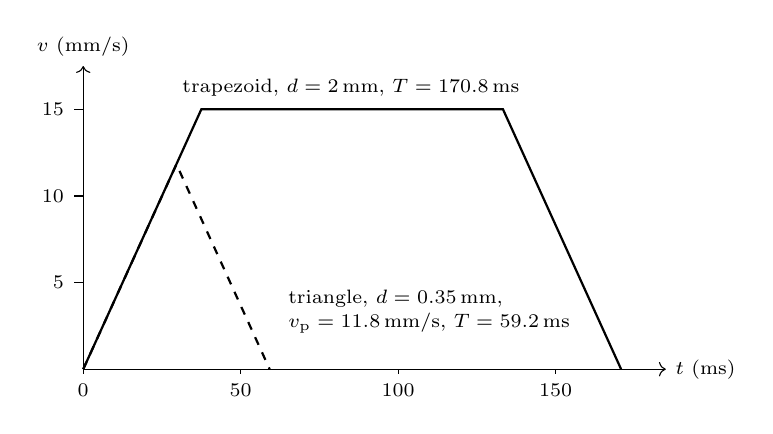
\begin{tikzpicture}[x=0.04cm,y=0.22cm]
\draw[->] (0,0) -- (185,0) node[right,font=\scriptsize] {$t$ (ms)};
\draw[->] (0,0) -- (0,17.5) node[above,font=\scriptsize] {$v$ (mm/s)};
\foreach \t in {0,50,100,150} {\draw (\t,0) -- (\t,-0.3) node[below,font=\scriptsize] {\t};}
\foreach \v in {5,10,15} {\draw (0,\v) -- (-3,\v) node[left,font=\scriptsize] {\v};}
\draw[thick] (0,0) -- (37.5,15) -- (133.3,15) -- (170.8,0);
\draw[thick,dashed] (0,0) -- (29.6,11.83) -- (59.2,0);
\node[font=\scriptsize,anchor=south] at (85,15.2) {trapezoid, $d=2$\,mm, $T=170.8$\,ms};
\node[font=\scriptsize,anchor=south west] at (62,3.0) {triangle, $d=0.35$\,mm,};
\node[font=\scriptsize,anchor=south west] at (62,1.5) {$v_{\mathrm p}=11.8$\,mm/s, $T=59.2$\,ms};
\end{tikzpicture}
\caption{Velocity profiles of Equation~\ref{eq:gc-trap} for $a=400$\,mm/s$^2$ and $v=15$\,mm/s: a 2\,mm move is trapezoidal (solid); the usual 0.35\,mm segment is triangular (dashed) and never reaches the cruise speed.}
\label{fig:gc-vel}
\end{figure}

\subsubsection{Verification of the program}
\label{sec:gc-verify}

An independent parser replays the file (it follows $X$ and $Y$, starts a polyline at \texttt{M3} and closes it at \texttt{M5}; only \texttt{G0} and \texttt{G1} are parsed, which suffices because nothing else is emitted).
The original trajectory (after placement and clamping) and the replayed polylines are rasterised on a common grid (8 pixels per millimetre), and the measures of Equation~\ref{eq:gc-verify} are reported:
\begin{equation}
\mathrm{IoU}=\frac{|M_{\mathrm t}\cap M_{\mathrm g}|}{|M_{\mathrm t}\cup M_{\mathrm g}|},\qquad e_{\mathrm{mean}}=\frac{1}{J}\sum_j\min_i\lVert g_j-s_i\rVert,\qquad e_{\max}=\max_j\min_i\lVert g_j-s_i\rVert
\label{eq:gc-verify}
\end{equation}
where $M_{\mathrm t}$ and $M_{\mathrm g}$ are the masks, $g_j$ the G-code vertices and $s_i$ the trajectory vertices (sub-sampled to at most 4000 and 6000).
The measure compares vertices with vertices and covers only the loss between trajectory and file (rounding, ordering, clamping), not the mechanical error (Section~\ref{sec:gan-res}).
The project notes quote $\mathrm{IoU}\approx0.99$ and a text-accuracy change of at most 0.3 percentage points between direct and read-back rendering (an earlier system state; Table~\ref{tab:syn-evid} shows later pairs), judged by the networks of the search; $e_{\mathrm{mean}}$ and $e_{\max}$ were not logged.
\mustdo{run the comparison for a set of generated programs and report $\mathrm{IoU}$, $e_{\mathrm{mean}}$, $e_{\max}$.}
\emph{Implementation note on the work area:} lines wrap at 185\,mm from $X_{\mathrm o}=10$\,mm, so a full-width line reaches $X=195$\,mm, but the driver clamps $X$ to 194\,mm and would distort the last millimetre; $X_{\max}$ or the line width should be reduced.


\subsection{Gantry control and hardware}
\label{sec:gantry}

This subsection describes the motion-control program and the hardware it drives (functional units FU~2.8 and FU~3.1 to FU~3.4; requirement R5). The single-board computer generates the step and direction pulses of both stepper drivers itself on its general-purpose pins, with no microcontroller in between.
The reason is that a move handed to a microcontroller cannot be interrupted without a round trip, whereas in the implemented design the loop that emits every step also reads the end-stop switches, so ``stop at once on any trigger'' is a property of the program; an earlier design with a microcontroller on a serial link was superseded for this reason.
The interpreter (about 800 lines of Python), the calibration and the safety logic were written by the student; the only library used gives access to the pins.

\subsubsection{Components, and why each was chosen}
\label{sec:gan-components}

Table~\ref{tab:gan-bom} lists the electrical and mechanical components and the reason each was selected. Every one was bought rather than designed, so no credit is claimed for the parts themselves; what is claimed is the selection, the interface circuits around them and the control program.
Table~\ref{tab:gan-pins} gives the pin assignment of the control program, and Table~\ref{tab:gan-hw} records, item by item, what the project files evidence --- including the transmission values the program assumes --- together with the information that must still be supplied.

\begin{table}[!htbp]
\centering
\fontsize{8.5}{10.2}\selectfont
\begin{tabularx}{\linewidth}{|>{\raggedright\arraybackslash}p{3.5cm}|>{\raggedright\arraybackslash}p{2.6cm}|>{\raggedright\arraybackslash}X|}
\hline
\textbf{Component} & \textbf{Quantity and rating} & \textbf{Reason for the choice} \\
\hline
Single-board computer, ODROID N2+ & 1 & The proposal requires all processing on an embedded platform. It runs the networks, the server and the motion control on one board, and its 3.3\,V pins are driven directly from the motion program. \\
\hline
Stepper motor, NEMA 17 & 2, 1.68\,A per phase~\cite{stepperds} & A stepper gives open-loop position from a step count~\cite{acarnley2002}, so no encoder is needed for the resolution R5 asks for. The NEMA 17 frame is the standard size for which the belts, pulleys and brackets used here are made. \mustdo{confirm the manufacturer, exact model number and datasheet revision or date of the stepper motors actually fitted, together with the rated phase current, step angle and the torque--speed curve; the bibliography entry carries none of these because the part could not be identified from the project files.} \\
\hline
Stepper driver, A4988 carrier~\cite{a4988ds} & 2 & Takes one STEP and one DIR line per axis, which is the smallest pin count for the job, and chops the coil current so the 1.68\,A winding can be run from the 24\,V rail. Microstepping to 1/16~\cite{acarnley2002,a4988ds} is set by jumpers and multiplies the resolution of Equation~\ref{eq:gan-spm} by sixteen. \mustdo{confirm the manufacturer, exact part number and datasheet revision or date of the driver carriers actually fitted (Allegro A4988 is assumed), since the carrier variant also fixes the sense-resistor value used in Equation~\ref{eq:gan-current}.} \\
\hline
Power supply & 1, 24\,V & A higher rail forces current into the winding inductance faster, which is what allows the step rates of Section~\ref{sec:gan-res}; 24\,V is inside the A4988's 8 to 35\,V input range~\cite{a4988ds}. \\
\hline
Bulk capacitor & 1, 100\,\textmu F & Supplies the switching current of the drivers locally so the rail does not sag at each chop (Equation~\ref{eq:gan-bulk}). \\
\hline
Micro switch & 5 & Four as the end-stops of the two axes, which make the direction-agnostic calibration of Section~\ref{sec:gan-calib} and the emergency stop possible; the fifth reports the state of the pen cam. A mechanical switch was chosen over an optical sensor because it needs no supply of its own and cannot be confused by ambient light. \\
\hline
Pull-down resistor & 4, 10\,k$\Omega$ & Holds each switch input low when the switch is open, so the input is never floating (Equation~\ref{eq:gan-pull}). \\
\hline
Pen-lift motor, N20 gear motor & 1, 150\,rpm & Geared down enough to turn the cam that toggles the pen in one direction. Its speed sets the toggle time, which Section~\ref{sec:gan-pen} shows is the largest single contributor to the predicted writing time. \\
\hline
Switching transistor, BC337-40, with 1\,k$\Omega$ base resistor & 1 & A general-purpose pin cannot supply the pen motor's current, so the pin switches the motor through a transistor instead (Equation~\ref{eq:gan-base} and Figure~\ref{fig:gan-pen-ckt}). \\
\hline
Timing belt and pulleys, GT2 2\,mm pitch, 20 teeth, with idler pulleys & 2 axes & A belt was chosen over a lead screw because the long, light travel of this machine needs speed more than it needs force, and because belt backlash can be kept small by tensioning with the idlers. 2\,mm pitch on 20 teeth gives the 40\,mm per revolution of Equation~\ref{eq:gan-spm}. \\
\hline
Chromed steel rods, linear bearings, 5\,mm to 8\,mm shaft coupler & as required & The rods and bearings carry the carriage so the belt only has to pull it, and the coupler joins the 5\,mm motor shaft to the 8\,mm cross-shaft described in Section~\ref{sec:gan-mech}. \\
\hline
USB camera in a printed housing & 1 & Fixes the camera at a known height above the page and clamps the paper flat, which is what makes the illumination correction of Section~\ref{sec:segmentation} work on a page that would otherwise curl. \\
\hline
\end{tabularx}
\caption{Components of the gantry and the capture rig, with the reason for each choice. All parts were bought; the interface circuits and the control program around them are the student's own work.}
\label{tab:gan-bom}
\end{table}

\mustcomplete{Add to Table~\ref{tab:gan-bom} the exact part numbers and the supplier of the motors,
the driver carrier boards, the power supply and the camera, together with the power supply's current
or VA rating, the camera's model and resolution, and the height at which the housing holds it above
the page. Also state how the 24\,V rail is converted to the voltages the ODROID~N2+ and the pen
motor need, because the board itself is not a 24\,V part and no converter is documented in the
project files.}

The twelve pins of Table~\ref{tab:gan-pins} are all the program needs: two outputs per axis, four switch inputs, and one input and one output for the pen mechanism. They are requested from \texttt{/dev/gpiochip0} in a single call, so a second instance of the program cannot claim the same pins while a job is running.

\begin{table}[!htbp]
\centering
\fontsize{9.5}{11.5}\selectfont
\begin{tabularx}{\linewidth}{|X|c|c|c|c|}
\hline
\textbf{Function} & \textbf{Offset} & \textbf{Header pin} & \textbf{Direction} & \textbf{Initial level} \\
\hline
X motor DIR / STEP & 64 / 68 & 7 / 11 & output & high / low \\
\hline
Y motor DIR / STEP & 81 / 69 & 12 / 13 & output & high / low \\
\hline
X\_MIN / X\_MAX switch & 72 / 65 & 15 / 16 & input & --- \\
\hline
Y\_MIN / Y\_MAX switch & 66 / 67 & 18 / 22 & input & --- \\
\hline
Pen-position switch & 70 & 33 & input & --- \\
\hline
Pen motor drive & 71 & 35 & output & low \\
\hline
\end{tabularx}
\caption{Pin assignment of the gantry driver on \texttt{/dev/gpiochip0}, requested in one call; the header pin numbers are those of the program comments and were not checked against the board pinout.}
\label{tab:gan-pins}
\end{table}

Table~\ref{tab:gan-hw} is the honest statement of how far the hardware description can be taken from the project files alone. Every entry marked in it is outstanding, and the two most serious gaps --- the power supply's rating and whether any level shifter lies between the 3.3\,V pins and the drivers --- bear directly on Section~\ref{sec:gan-supply}.

\begin{table}[!htbp]
\centering
\fontsize{9.5}{11.5}\selectfont
\begin{tabularx}{\linewidth}{|p{2.6cm}|X|}
\hline
\textbf{Item} & \textbf{Evidence, and content to be supplied} \\
\hline
Computer & ODROID N2+ with 3.3\,V pins (Table~\ref{tab:gan-pins}). \\
\hline
Motors, drivers, transmission & Two motors with STEP/DIR driver modules; the program assumes 200 full steps per revolution~\cite{stepperds}, an A4988 at 1/16 microstepping~\cite{a4988ds} and 40\,mm per revolution (2\,mm belt, 20-tooth pulley), and replaces the last by calibration. \mustdo{motor model, holding torque, rated current; driver model, current-limit setting, microstepping jumpers, minimum STEP pulse width; belt or screw type, pulley teeth, guides; whether any level shifter lies between the 3.3\,V pins and the drivers.} \\
\hline
Travel & Measured switch-to-switch distances 204\,mm (X) and 262\,mm (Y). \mustdo{the calibrated steps per millimetre printed for both axes.} \\
\hline
End-stops & Four switches, active-high at 3.3\,V, each with a pull-down of about 10\,k$\Omega$ (Figure~\ref{fig:gan-switch}). \mustdo{switch type and mounting.} \\
\hline
Pen mechanism & One-direction gear motor whose cam toggles the pen every $90^\circ$, with a pen switch (high = up) (Section~\ref{sec:gan-pen}). \mustdo{how the motor is switched (transistor, flyback diode), supply voltage, pen model and holder, lift height.} \\
\hline
Power supply (FU 4) & \mustdo{voltages and current ratings of the motor, computer and pen-motor supplies, grounding scheme, camera supply.} The program comments state that the motors have no flyback diodes and share a ground return, which makes the switch inputs noisy (Section~\ref{sec:gan-stop}). \\
\hline
Camera (FU 1) & Generic USB video-class camera. \mustdo{model, resolution, mounting height, field of view, lamp.} \\
\hline
\end{tabularx}
\caption{Hardware items: evidence in the project files and information still to be supplied.}
\label{tab:gan-hw}
\end{table}

\subsubsection{Mechanical arrangement}
\label{sec:gan-mech}

The machine is a Cartesian gantry of two axes, one motor and one belt each, and the chain is best followed body by body.
The lower axis carries the whole upper axis and is driven by one motor whose shaft is joined, through the 5\,mm to 8\,mm coupler, to an 8\,mm cross-shaft spanning the frame.
That one shaft turns a pulley at each end, so both sides of the moving bridge are driven from the same motor and advance by the same amount; this is what keeps the bridge square to the frame without a second motor and without the electronic synchronisation two motors would need.
The second motor rides on that bridge and drives a single pulley, which moves the carriage along the bridge.
The pen-lift motor and its cam ride on that carriage, so the pen is the last body in the chain and the only mass that has to be moved by the smaller of the two belt loops.
All moving parts run on linear bearings over chromed steel rods, and each belt is tensioned against an idler pulley.

Putting the second motor on the moving bridge is the main mechanical trade-off of the design: it keeps each axis to one motor and one belt, but the lower axis then has to accelerate the upper motor's mass as well as the carriage, which lowers the acceleration that axis can reach before it loses steps.
The alternative, a fixed second motor with a longer belt routed through the bridge, removes that mass but adds idlers and a belt path that changes length as the bridge moves.
The simpler arrangement was chosen because the writing speed turned out to be limited by the search in Section~\ref{sec:synthesis} and by the pen toggle, not by how fast the axes can be accelerated.

The torque each motor must supply follows from the pulley's pitch radius.
For a belt of pitch $p$ on a pulley of $N_t$ teeth the travel per revolution and the pitch radius are given by Equation~\ref{eq:gan-radius},
\begin{equation}
\ell_{\mathrm{rev}}=p\,N_t=2\cdot20=40\ \mathrm{mm},\qquad r=\frac{\ell_{\mathrm{rev}}}{2\pi}=\frac{40}{2\pi}=6.37\ \mathrm{mm},
\label{eq:gan-radius}
\end{equation}
From the pitch radius of Equation~\ref{eq:gan-radius}, the torque needed to accelerate a carriage of mass $m$ at acceleration $a$ against a friction force $F_f$ is
\begin{equation}
T=r\,(m\,a+F_f).
\label{eq:gan-torque}
\end{equation}
Equation~\ref{eq:gan-torque} is the check that decides whether the motors can follow the step rates of Section~\ref{sec:gan-res} without stalling, and it is the calculation this design is missing: neither the carriage masses nor the friction force was measured, and the motors' pull-out torque at the rates used~\cite{acarnley2002,stepperds} was not obtained, so no torque margin can be stated.
This is the reason the program uses no acceleration ramp and why Section~\ref{sec:gan-res} can only warn that abrupt starts may lose steps.

Figure~\ref{fig:gan-photo} is the place where the photographs of the built machine belong. They are design evidence rather than decoration, because the mechanical chain above and the component choices of Table~\ref{tab:gan-bom} can only be checked against the assembled gantry, and the folder intended for them in the project files is empty.

\begin{figure}[!htbp]
\centering
\figplaceholder{2.4cm}{Photographs of the assembled gantry (axes, end-stops, pen holder with toggle motor, paper holder) and of the scanning rig with camera; CAD renderings and a wiring diagram with component values. To be supplied by the student.}
\caption{Photographs of the gantry and the scanning rig (placeholder).}
\label{fig:gan-photo}
\end{figure}

\mustdo{Weigh the two carriages and measure or estimate the friction force, then evaluate
Equation~\ref{eq:gan-torque} at the 400\,mm/s$^2$ of Equation~\ref{eq:gc-trap} and compare the result
with the pull-out torque of the motors at 1200 and 3200 steps per second taken from their torque-speed
curve. State the resulting margin. Also insert the CAD drawings of the gantry and the camera housing
and the photographs of the built machine (Figure~\ref{fig:gan-photo}); the folder intended for them in
the project files is empty, so nothing could be reproduced here.}

\subsubsection{Stepper driver and the coil-current setting}
\label{sec:gan-driver}

Each driver is wired as in Figure~\ref{fig:gan-wiring}: the 24\,V rail and the bulk capacitor to the motor supply pins, the four coil wires to the two output pairs, and STEP and DIR to two pins of the single-board computer. The A4988 chops the coil current, and the current it regulates to is set by a trimmer reference voltage together with the two current-sense resistors of the carrier board, Equation~\ref{eq:gan-current}, which is the relation given in the driver's datasheet~\cite{a4988ds},
\begin{equation}
I_{\mathrm{coil}}=\frac{V_{\mathrm{ref}}}{8\,R_S}\qquad\Longrightarrow\qquad V_{\mathrm{ref}}=8\,R_S\,I_{\mathrm{coil}}.
\label{eq:gan-current}
\end{equation}
For the 1.68\,A rating of these motors and the 0.1\,$\Omega$ sense resistors most commonly fitted to these carriers, Equation~\ref{eq:gan-current} asks for $V_{\mathrm{ref}}=8\cdot0.1\cdot1.68=1.34$\,V.
The motors should not in fact be run at their full rating on this driver.
The current the A4988 regulates to flows through the driver's output transistors, and the heat it produces, $P\approx2I_{\mathrm{coil}}^2R_{DS(\mathrm{on})}$ per driver, has only the small carrier board to leave through, which is why a carrier without a heatsink or forced air is usually held to about 1\,A per phase rather than to the 1.68\,A of Equation~\ref{eq:gan-current}.
Accordingly $V_{\mathrm{ref}}$ is set to about $0.8$\,V on a 0.1\,$\Omega$ board, which trades holding torque for a driver that does not go into thermal shutdown part way through a page; losing a step to an overheating driver costs more accuracy than the lower holding torque does.

\mustdo{Confirm three things about Equation~\ref{eq:gan-current}, because the setting cannot be
read back from the program. First, the sense-resistor value actually fitted to these carrier boards
(0.05, 0.068 and 0.1\,$\Omega$ are all sold) --- read it off the board or measure it. Second, the
voltage the trimmer is actually set to, measured at the reference pin with a multimeter, and the coil
current that Equation~\ref{eq:gan-current} then gives. Third, whether the drivers have heatsinks or a
fan, and whether a thermal shutdown was ever observed during a long job. State the resulting coil
current as a fraction of the 1.68\,A rating.}

\subsubsection{Switch inputs}
\label{sec:gan-switch}

Figure~\ref{fig:gan-switch-ckt} shows one switch input; all five are identical. The switch connects the pin to 3.3\,V when it closes, and a 10\,k$\Omega$ resistor to ground holds the pin low when it is open, so the input is defined at all times.
The current drawn while a switch is closed and the worst case with all four end-stops closed follow from Ohm's law, Equation~\ref{eq:gan-pull},
\begin{equation}
I_{\mathrm{pull}}=\frac{V_{DD}}{R}=\frac{3.3}{10\,000}=0.33\ \mathrm{mA},\qquad 4I_{\mathrm{pull}}=1.3\ \mathrm{mA},
\label{eq:gan-pull}
\end{equation}
which is negligible against anything else on the board.
The choice of 10\,k$\Omega$ is bounded from both sides.
Making the pull-down resistor of Equation~\ref{eq:gan-pull} much smaller than 10\,k$\Omega$ wastes current for no benefit; making it much larger lets the pin's own leakage current $I_{\mathrm{leak}}$ lift the open-switch voltage, and to keep that below the input's low threshold $V_{IL}$ the resistor must satisfy $R\le V_{IL}/I_{\mathrm{leak}}$, both quantities being properties of the single-board computer's pins~\cite{odroidn2ds} \mustdo{confirm the exact ODROID-N2+ board revision and the document (hardware technical reference or datasheet) and its date from which $V_{IL}$ and the input leakage current are taken; the bibliography entry carries no revision or date because the board variant could not be confirmed.}.
The resistor also forms a low-pass filter with the pin and cable capacitance, with time constant $\tau_{RC}=R\,(C_{\mathrm{in}}+C_{\mathrm{cable}})$; for 10\,k$\Omega$ and any plausible stray capacitance of tens to hundreds of picofarads this is a few microseconds, which is more than three orders of magnitude below the 6\,ms between the repeated reads of Section~\ref{sec:gan-stop}, so the debounce is entirely a property of the program and not of this circuit.
Figure~\ref{fig:gan-switch} draws the same input as it is documented in the program comments, with the 0.33\,mA of Equation~\ref{eq:gan-pull} marked on it; the origin of the 3.3\,V at the switch is inferred from those comments rather than read off the board, which is why the figure carries a marker of its own.

\begin{figure}[!htbp]
\centering
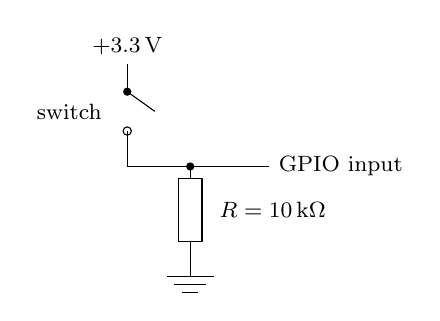
\begin{tikzpicture}[x=1cm,y=1cm,font=\footnotesize]
\draw (0,1.9) node[above] {$+3.3$\,V} -- (0,1.55);
\fill (0,1.55) circle (1.5pt); \draw (0,1.55) -- (0.35,1.3); \draw (0,1.05) circle (1.5pt); \draw (0,1.05) -- (0,0.6);
\node[anchor=east] at (-0.2,1.3) {switch};
\draw (0,0.6) -- (1.8,0.6) node[right] {GPIO input};
\fill (0.8,0.6) circle (1.5pt);
\draw (0.8,0.6) -- (0.8,0.45); \draw[fill=white] (0.65,0.45) rectangle (0.95,-0.35); \draw (0.8,-0.35) -- (0.8,-0.8);
\node[anchor=west] at (1.05,0.05) {$R=10$\,k$\Omega$};
\draw (0.5,-0.8) -- (1.1,-0.8); \draw (0.6,-0.9) -- (1.0,-0.9); \draw (0.7,-1.0) -- (0.9,-1.0);
\end{tikzpicture}
\caption{Switch input circuit as documented in the program comments; the closing current is $3.3\,\mathrm{V}/10\,\mathrm{k}\Omega=0.33$\,mA. The origin of the 3.3\,V (header pin) is inferred and \mustdo{confirm this item}.}
\label{fig:gan-switch}
\end{figure}

The electrical weakness of this arrangement is the return path rather than the resistor.
The motors have no clamp diodes and share a ground return with the switch wiring, so each time a coil is switched its current has to find a path back through that shared conductor: a current $I$ returning through a ground conductor of resistance $R_{gnd}$ raises the local ground by $I\,R_{gnd}$, and the switch inputs are referred to that same ground, so the apparent switch voltage is offset by the same amount.
This is the mechanism behind the behaviour recorded in Section~\ref{sec:gan-stop}, where an input was found to read high for several milliseconds after a motor switched, and it is why a single re-read was not enough and three reads 6\,ms apart were needed.
The correct fix is electrical, not a longer debounce: a clamp diode across each motor, and a switch return brought back to a single ground point separately from the motor current.

\mustdo{For Equation~\ref{eq:gan-pull}, take $V_{IL}$ and the input leakage current from the
ODROID~N2+ documentation~\cite{odroidn2ds} and state the resulting upper bound on the pull-down resistor, so the choice
of 10\,k$\Omega$ is bounded by numbers rather than by argument. Confirm also that each switch is wired
to 3.3\,V and not to 5\,V, since the program reads the inputs as active-high at 3.3\,V.}

\subsubsection{Pen-lift motor and its switching stage}
\label{sec:gan-penckt}

A general-purpose pin can source only a few milliamperes, far below what even a small geared motor draws, so the pen motor is switched by a transistor on the low side as in Figure~\ref{fig:gan-pen-ckt}, the pin driving the base through a 1\,k$\Omega$ resistor. With the pin at 3.3\,V and the base-emitter drop of a saturated small-signal transistor taken as 0.7\,V~\cite{bc337ds} \mustdo{confirm the manufacturer (onsemi and Nexperia both supply this part), the exact part number and the datasheet revision or date of the transistor actually fitted, and check the gain group, $V_{BE(\mathrm{sat})}$, $V_{CE(\mathrm{sat})}$ and TO-92 power dissipation used below against that document; the bibliography entry carries no revision because the variant could not be identified.}, the base current is given by Equation~\ref{eq:gan-base},
\begin{equation}
I_B=\frac{V_{\mathrm{pin}}-V_{BE(\mathrm{sat})}}{R_B}=\frac{3.3-0.7}{1000}=2.6\ \mathrm{mA}.
\label{eq:gan-base}
\end{equation}
The BC337-40 belongs to the $-40$ gain group, whose minimum current gain is 250~\cite{bc337ds}, and to hold it in saturation rather than use it as an amplifier the base must be driven harder than the collector current strictly requires, by an overdrive factor $k_{od}$ of three to five, so the collector current the stage can switch is given by Equation~\ref{eq:gan-ic},
\begin{equation}
I_{C(\max)}=\frac{h_{FE(\min)}\,I_B}{k_{od}}=\frac{250\cdot2.6\ \mathrm{mA}}{k_{od}}=\frac{650\ \mathrm{mA}}{k_{od}},
\label{eq:gan-ic}
\end{equation}
which is 217\,mA at $k_{od}=3$ and 130\,mA at $k_{od}=5$.
The stage is therefore comfortable for a motor drawing up to about 200\,mA and would leave saturation, and begin to dissipate real power, somewhere above that.
The dissipation in the transistor while saturated is $P=V_{CE(\mathrm{sat})}I_C$, which at 200\,mA and a saturation voltage of about 0.7\,V is 0.14\,W, well inside what the TO-92 package can lose without a heatsink~\cite{bc337ds}.

Two things about this stage are not right, and both are stated here rather than in the discussion because they are design faults and not merely untested items.
First, there is no clamp diode across the motor: when the transistor turns off, the energy $\tfrac12LI^2$ stored in the motor's inductance has nowhere to go and appears as a reverse voltage that both stresses the transistor and injects the noise that Section~\ref{sec:gan-switch} describes. A diode across the motor, cathode to the supply, rated for at least the motor current and twice the motor supply voltage, is the standard remedy and was omitted.
Second, there is no base pull-down: the base resistor leaves the base floating while the pin is in its power-up input state, so a pull-down from base to emitter should be fitted to guarantee the motor is off before the program claims the pin.

\mustdo{Measure the pen motor's free-running current and its stall current, then check them
against Equation~\ref{eq:gan-ic}: if the stall current is above about 200\,mA the stage is not hard
saturated and the base resistor should be reduced. State the voltage the pen motor is actually run
from. Confirm whether a clamp diode and a base pull-down were in fact fitted, since neither appears in
the project files; if they were not, this subsection is correct as written and the omission belongs in
Section~\ref{sec:discussion}.}

\subsubsection{Supply and decoupling}
\label{sec:gan-supply}

The 24\,V rail feeds both drivers, and a 100\,\textmu F capacitor is fitted across it close to them to supply the switching current locally, because the chopper in each driver draws current in bursts that the supply leads, which have inductance of their own, cannot follow.
For a current step $I$ lasting $\Delta t$ the rail sags by the amount of Equation~\ref{eq:gan-bulk},
\begin{equation}
\Delta V=\frac{I\,\Delta t}{C},
\label{eq:gan-bulk}
\end{equation}
so a 1.68\,A step lasting 10\,\textmu s drawn from 100\,\textmu F costs $1.68\cdot10\times10^{-6}/100\times10^{-6}=0.17$\,V, which is small against 24\,V and comfortably clear of the driver's undervoltage threshold.
Two gaps remain.
The 100\,\textmu F is shared between the two drivers, whereas the usual recommendation is a bulk capacitor of this order at each driver; and no small ceramic capacitor on the logic supply of either driver is documented, which is the part that suppresses the fast edges rather than the bulk current.
The total supply current also has not been budgeted: it is the sum of two motors at two phases each, the pen motor, the single-board computer and the camera, and without the supply's rating the margin is unknown.

\mustdo{Give the power supply's voltage and current rating and complete the power budget: two
motors at two phases each at the coil current set in Section~\ref{sec:gan-driver}, plus the pen motor,
the ODROID~N2+ and the camera. State the margin that remains. Confirm whether each driver has its own
bulk capacitor and whether a ceramic capacitor is fitted on either driver's logic supply.}

A separate check belongs here because it bears on the only hardware fault in this report.
The driver's STEP, DIR and enable inputs are driven straight from 3.3\,V pins, with no level shifting.
Whether that is correct depends on the voltage the driver needs to see as a logic high, $V_{IH}$, which the driver's datasheet specifies relative to the driver's own logic supply~\cite{a4988ds}: the design is sound if $3.3\,\mathrm{V}>V_{IH}$ with margin, and marginal if it is not.
During commissioning the X axis drove to its first end-stop but the direction pin was not observed to change level on reversal, and that fault was not resolved (Section~\ref{sec:results}).
A level incompatibility is one candidate explanation, but a wiring or configuration fault, a damaged pin and a program fault are equally consistent with what was seen, and no measurement was taken that would separate them.
No cause is claimed here.

\mustcomplete{Resolve the X-axis direction fault, which currently blocks requirement R5 entirely.
Take $V_{IH}$ for the driver's logic inputs from its datasheet and compare it with 3.3\,V to settle
whether level shifting is needed. Then put a meter or a scope on the DIR pin at the pin and again at
the driver, command a reversal, and record whether the level changes at each point. That single
measurement separates a program fault from a wiring fault from a level-compatibility fault, and
nothing further can be said about R5 until it is done.}

\begin{figure}[!htbp]
\centering
\scalebox{0.88}{%
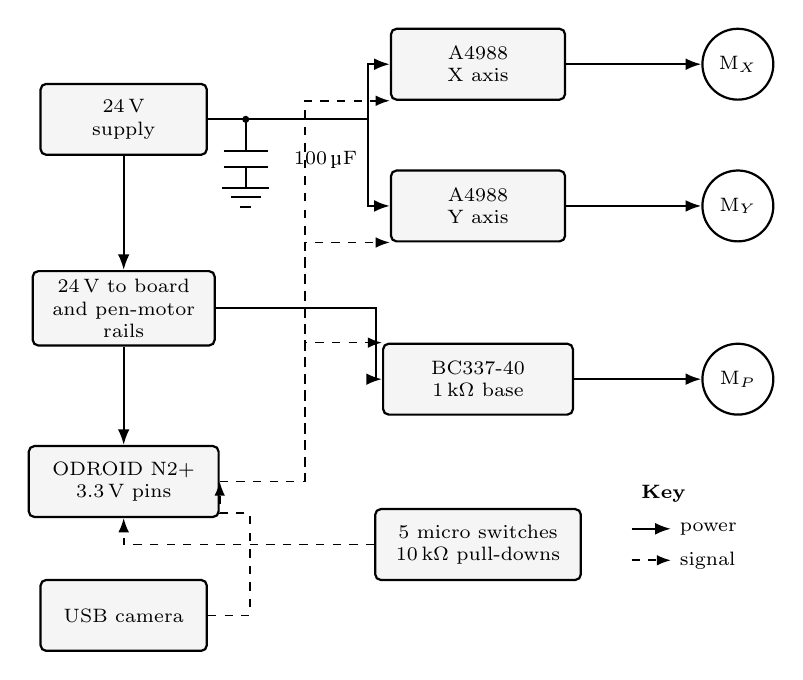
\begin{tikzpicture}[x=1cm,y=1cm,font=\scriptsize,>=latex]
\tikzset{
  blk/.style={draw,thick,rounded corners=2pt,align=center,minimum height=9mm,inner sep=3pt,fill=gray!8},
  mot/.style={draw,thick,circle,minimum size=9mm,fill=white},
  wire/.style={draw,thick},
  pwr/.style={draw,thick,-{Latex[length=2mm]}},
  sig/.style={draw,semithick,-{Latex[length=1.8mm]},dashed}
}
\node[blk,text width=1.9cm] (psu) at (0,0) {24\,V\\supply};
\node[blk,text width=2.1cm] (conv) at (0,-2.4) {24\,V to board\\and pen-motor\\rails};
\node[blk,text width=2.2cm] (sbc) at (0,-4.6) {ODROID N2+\\3.3\,V pins};
\node[blk,text width=2.0cm] (dx) at (4.5,0.7) {A4988\\X axis};
\node[blk,text width=2.0cm] (dy) at (4.5,-1.1) {A4988\\Y axis};
\node[mot] (mx) at (7.8,0.7) {M$_X$};
\node[mot] (my) at (7.8,-1.1) {M$_Y$};
\node[blk,text width=2.2cm] (pen) at (4.5,-3.3) {BC337-40\\1\,k$\Omega$ base};
\node[mot] (pm) at (7.8,-3.3) {M$_P$};
\node[blk,text width=2.4cm] (sw) at (4.5,-5.4) {5 micro switches\\10\,k$\Omega$ pull-downs};
\node[blk,text width=1.9cm] (cam) at (0,-6.3) {USB camera};
% bulk capacitor: shunts the 24 V rail to ground
\draw[wire] (1.55,0) -- (1.55,-0.40);
\draw[wire] (1.27,-0.40) -- (1.83,-0.40);
\draw[wire] (1.27,-0.61) -- (1.83,-0.61);
\draw[wire] (1.55,-0.61) -- (1.55,-0.87);
\draw[wire] (1.25,-0.87) -- (1.85,-0.87);
\draw[wire] (1.36,-0.99) -- (1.74,-0.99);
\draw[wire] (1.48,-1.11) -- (1.62,-1.11);
\node[right,inner sep=3pt] at (2.05,-0.51) {100\,\textmu F};
\fill (1.55,0) circle (0.045);
% power routing
\draw[pwr] (psu.east) -- (3.1,0) |- (dx.west);
\draw[pwr] (3.1,0) |- (dy.west);
\draw[pwr] (psu.south) -- (conv.north);
\draw[pwr] (conv.south) -- (sbc.north);
\draw[pwr] (conv.east) -| (3.2,-3.3) -- (pen.west);
\draw[pwr] (dx.east) -- (mx.west);
\draw[pwr] (dy.east) -- (my.west);
\draw[pwr] (pen.east) -- (pm.west);
% signals
\draw[sig] (sbc.east) -- (2.3,-4.6) |- (dx.south west);
\draw[sig] (2.3,-4.6) |- (dy.south west);
\draw[sig] (2.3,-4.6) |- (pen.north west);
\draw[sig] (sw.west) -- (2.7,-5.4) -| (sbc.south);
\draw[sig] (cam.east) -- (1.6,-6.3) -- (1.6,-5.0) -| (sbc.east);
\node[anchor=west] at (6.45,-4.75) {\textbf{Key}};
\draw[pwr] (6.45,-5.20) -- (6.95,-5.20); \node[right,inner sep=3pt] at (6.95,-5.20) {power};
\draw[sig] (6.45,-5.60) -- (6.95,-5.60); \node[right,inner sep=3pt] at (6.95,-5.60) {signal};
\end{tikzpicture}}
\caption{Wiring of the electronics. The 24\,V rail feeds both drivers and is decoupled by the 100\,\textmu F capacitor of Equation~\ref{eq:gan-bulk}; the board drives STEP and DIR of each driver and the pen-motor transistor's base, and reads the five switches. The conversion from 24\,V to the voltages the board and the pen motor need is not documented in the project files.}
\label{fig:gan-wiring}
\end{figure}

\begin{figure}[!htbp]
\centering
\scalebox{0.88}{%
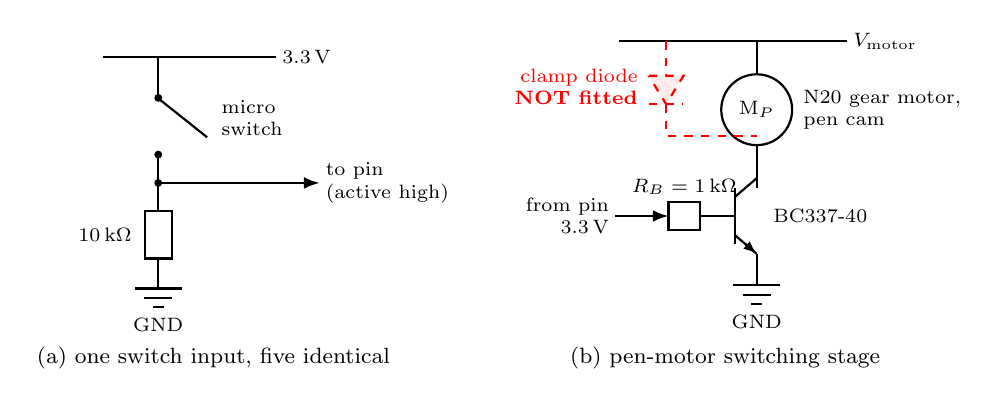
\begin{tikzpicture}[x=1cm,y=1cm,font=\scriptsize,>=latex]
%% ---------------- (a) switch input ----------------
\begin{scope}
\draw[thick] (-0.7,2.4) -- (1.5,2.4);
\node[right,inner sep=2pt] at (1.5,2.4) {3.3\,V};
\draw[thick] (0,2.4) -- (0,1.88);
\fill (0,1.88) circle (0.05);
\draw[thick] (0.03,1.85) -- (0.62,1.38);
\fill (0,1.16) circle (0.05);
\draw[thick] (0,1.16) -- (0,0.80);
\node[right,align=left] at (0.68,1.62) {micro\\switch};
\fill (0,0.80) circle (0.05);
\draw[thick] (0,0.80) -- (1.45,0.80);
\draw[thick,-{Latex[length=2mm]}] (1.45,0.80) -- (2.05,0.80);
\node[right,align=left,inner sep=2pt] at (2.05,0.80) {to pin\\(active high)};
\draw[thick] (0,0.80) -- (0,0.44);
\draw[thick,fill=white] (-0.17,0.44) rectangle (0.17,-0.16);
\node[left,inner sep=4pt] at (-0.19,0.14) {$10\,\mathrm{k}\Omega$};
\draw[thick] (0,-0.16) -- (0,-0.54);
\draw[thick] (-0.30,-0.54) -- (0.30,-0.54);
\draw[thick] (-0.18,-0.66) -- (0.18,-0.66);
\draw[thick] (-0.07,-0.78) -- (0.07,-0.78);
\node[below,inner sep=3pt] at (0,-0.81) {GND};
\node[font=\footnotesize] at (0.7,-1.42) {(a) one switch input, five identical};
\end{scope}
%% ---------------- (b) pen-motor switching stage ----------------
\begin{scope}[xshift=7.6cm]
\draw[thick] (-1.75,2.6) -- (1.15,2.6);
\node[right,inner sep=2pt] at (1.15,2.6) {$V_{\mathrm{motor}}$};
% motor
\draw[thick] (0,2.6) -- (0,2.18);
\node[draw,thick,circle,minimum size=9mm,fill=white] at (0,1.73) {M$_P$};
\draw[thick] (0,1.28) -- (0,0.88);
\node[right,align=left,inner sep=3pt] at (0.48,1.73) {N20 gear motor,\\pen cam};
% clamp diode, drawn dashed because it is NOT fitted
\draw[red,dashed,thick] (-1.15,2.6) -- (-1.15,2.16);
\draw[red,dashed,thick,fill=red!8] (-1.37,2.16) -- (-0.93,2.16) -- (-1.15,1.80) -- cycle;
\draw[red,dashed,thick] (-1.37,1.80) -- (-0.93,1.80);
\draw[red,dashed,thick] (-1.15,1.80) -- (-1.15,1.40) -- (0,1.40);
\node[left,align=right,red,inner sep=3pt] at (-1.40,2.02) {clamp diode\\\textbf{NOT fitted}};
% NPN transistor
\draw[thick] (0,0.88) -- (0,0.74);
\draw[thick] (-0.28,0.74) -- (-0.28,0.02);
\draw[thick] (-0.28,0.62) -- (0,0.86);
\draw[thick] (-0.28,0.14) -- (0,-0.10);
\draw[thick,-{Latex[length=1.7mm]}] (-0.15,0.03) -- (0,-0.10);
\draw[thick] (0,-0.10) -- (0,-0.50);
\node[right,inner sep=3pt] at (0.10,0.38) {BC337-40};
% base drive, arrow pointing INTO the base resistor
\draw[thick] (-0.28,0.38) -- (-0.72,0.38);
\draw[thick,fill=white] (-1.12,0.20) rectangle (-0.72,0.56);
\node[above,inner sep=2pt] at (-0.92,0.57) {$R_B=1\,\mathrm{k}\Omega$};
\draw[thick,-{Latex[length=2mm]}] (-1.80,0.38) -- (-1.12,0.38);
\node[left,align=right,inner sep=2pt] at (-1.80,0.38) {from pin\\3.3\,V};
% ground
\draw[thick] (-0.30,-0.50) -- (0.30,-0.50);
\draw[thick] (-0.18,-0.62) -- (0.18,-0.62);
\draw[thick] (-0.07,-0.74) -- (0.07,-0.74);
\node[below,inner sep=3pt] at (0,-0.77) {GND};
\node[font=\footnotesize] at (-0.4,-1.42) {(b) pen-motor switching stage};
\end{scope}
\end{tikzpicture}}
\caption{The two interface circuits designed around the bought parts. In (a) the 10\,k$\Omega$ resistor holds the pin at ground until the switch closes, drawing the 0.33\,mA of Equation~\ref{eq:gan-pull}; in (b) the pin drives the base through 1\,k$\Omega$, giving the 2.6\,mA of Equation~\ref{eq:gan-base} and the collector current of Equation~\ref{eq:gan-ic}. The clamp diode shown dashed is the standard protection against the motor's inductive turn-off; it is not fitted in the built circuit, and its absence is the source of the switch-input disturbance of Section~\ref{sec:gan-switch}.}
\label{fig:gan-switch-ckt}
\label{fig:gan-pen-ckt}
\end{figure}

\subsubsection{Step generation, resolution and speed}
\label{sec:gan-res}

A driver advances the motor one microstep per pulse at STEP, in the direction given by DIR.
With 200 full steps~\cite{stepperds}, 16 microsteps per step~\cite{a4988ds} and $\ell_{\mathrm{rev}}=40$\,mm per revolution (assumed values), Equation~\ref{eq:gan-spm} gives the step resolution,
\begin{equation}
\kappa=\frac{200\cdot16}{\ell_{\mathrm{rev}}}=\frac{3200}{40}=80\ \mathrm{steps/mm},\qquad\Delta=\frac1\kappa=12.5\ \mu\mathrm{m},
\label{eq:gan-spm}
\end{equation}
and after calibration $\kappa$ is replaced by the measured value of each axis.
Targets are converted to \emph{absolute} integer step counts, $n_{\mathrm{target}}=\mathrm{round}\bigl((x+5)\kappa\bigr)$ with the 5\,mm edge offset of Section~\ref{sec:gan-calib} and the calibrated resolution $\kappa$ of Equation~\ref{eq:gan-cal}, and the step difference is taken against the tracked integer position, so rounding errors do not accumulate.
The quantisation error is at most $\Delta/2=6.25\ \mu$m per axis and $\sqrt2\,\Delta/2=8.8\ \mu$m combined, 57 times finer than the 0.5\,mm of R5.
This is only the \emph{digital} resolution: the accuracy of a mark is set by belt stretch, backlash, missed steps (open loop, no encoders), switch repeatability and pen compliance, none of which was measured.
\mustdo{measure the positional error for R5 (the same word drawn twice and overlaid) and the return-to-zero repeatability.}

For a move of length $d$ at feed $v_f$ (mm/s) with $N_{\mathrm{maj}}=\max(|n_x|,|n_y|,1)$ steps on the major axis the delay of every pulse is given by Equation~\ref{eq:gan-tau},
\begin{equation}
\tau=\max\Bigl(\frac{d/v_f}{N_{\mathrm{maj}}},\ 2\,\mu\mathrm s\Bigr),\qquad v_f=\max(F/60,\,0.1),
\label{eq:gan-tau}
\end{equation}
with $F$ the feed in mm/min.
For an axis-parallel move, 900\,mm/min gives $\tau=1/(15\cdot80)=833\ \mu$s (1200 steps/s) and 2400\,mm/min gives 312.5\,\textmu s (3200 steps/s, 60\,rpm), while homing and retracting run at 625 steps/s or $7.8$\,mm/s. The real rate is limited by the program (four switch readings and two pin writes per step) and the sleep granularity, not by the 2\,\textmu s floor; the maximum reliable rate and the stall speed were not measured.
\mustdo{measure the highest feed without lost steps.}
Since \emph{every} pulse of both axes sleeps for $\tau$, a segment takes $(n_{\mathrm{maj}}+n_{\mathrm{min}})\tau$ and the effective feed is given by Equation~\ref{eq:gan-eff},
\begin{equation}
v_{\mathrm{eff}}=v_f\,\frac{n_{\mathrm{maj}}}{n_{\mathrm{maj}}+n_{\mathrm{min}}}\in\Bigl[\frac{v_f}{2},v_f\Bigr],
\label{eq:gan-eff}
\end{equation}
$v_f$ for an axis-parallel move and $v_f/2$ at $45^\circ$; for uniformly distributed directions the mean factor is $\frac4\pi\int_0^{\pi/4}\frac{\mathrm d\vartheta}{1+\tan\vartheta}=\frac12+\frac{\ln2}{\pi}=0.72$.
The interpreter executes \emph{no acceleration ramps}: the constant speed of Equation~\ref{eq:gan-tau} is used, and the acceleration of Equation~\ref{eq:gc-trap} appears only in the generator's estimate; abrupt starts at 1200 to 3200 steps/s with an unknown motor and load may lose steps, which is exactly the failure that controlled acceleration within the torque--speed envelope is meant to prevent in an open-loop drive~\cite{acarnley2002}.
\label{sec:gan-timing}
A model of the interpreter for the test word of Section~\ref{sec:gcode} (modal feed, Equation~\ref{eq:gan-eff}, first travel at 2400\,mm/min) gives 6.8\,s drawing, 10.8\,s travel and 9.1\,s dwell, 26.7\,s in total (2.4\,s per character for 11 characters), so dwell is 34\,\% of the predicted time.
Neither this nor Equation~\ref{eq:gc-trap} includes the pen-motor run time or program overhead, and neither is a measurement; both are below the 4\,s per character of R3 for this short word, but R3 must be demonstrated with a stopwatch.

\subsubsection{Bresenham line interpolation}

Stepping the two axes independently would draw an L-shaped path, so the program uses the integer algorithm of Bresenham~\cite{bresenham1965}, which carries an error term $e$ along the major axis of $a_x=|\Delta x|$ and $a_y=|\Delta y|$ steps, pulses STEP of the major axis once per iteration and pulses the minor axis whenever $e$ would go negative, reading the end-stops before every major-axis step.
With those two step counts and the DIR pins set once, the loop runs as follows for $a_x\ge a_y$ (else the roles swap): (1) set $e\leftarrow\lfloor a_x/2\rfloor$; (2) repeat $a_x$ times: if an end-stop is triggered, stop; pulse STEP of X; $e\leftarrow e-a_y$; if $e<0$, pulse STEP of Y and $e\leftarrow e+a_x$.
The error term $e$ is the quantity whose bound gives Equation~\ref{eq:gan-bres}: keeping $e=\lfloor a_x/2\rfloor-k\,a_y+m_ka_x$ in $[0,a_x)$ gives, after $k$ major steps, the minor-axis count,
\begin{equation}
m_k=\Bigl\lceil\frac{k\,a_y-\lfloor a_x/2\rfloor}{a_x}\Bigr\rceil,
\label{eq:gan-bres}
\end{equation}
which differs from the ideal $k\,a_y/a_x$ by at most $\tfrac12+\tfrac1{2a_x}\le1$ step (about 6\,\textmu m); only integer arithmetic is needed.

\subsubsection{Direction-agnostic calibration}
\label{sec:gan-calib}

Equation~\ref{eq:gan-spm} rests on assumed transmission values and the position after power-up is unknown, so each session starts with a calibration between the two switches of each axis, which never needs to know which direction leads to which switch: for one axis the program drives in an arbitrary direction (DIR high, 1.6\,ms per step) until \emph{either} switch triggers, reverses, and counts the steps $N$ until the \emph{other} switch triggers.
With the hand-measured switch-to-switch travel $L$ (204\,mm in X, 262\,mm in Y), the calibrated resolution, the initial counter and the position in millimetres are given by Equation~\ref{eq:gan-cal},
\begin{equation}
\kappa_{\mathrm{axis}}=\frac{N}{L},\qquad n_0=\begin{cases}N&\text{if the second switch was MAX,}\\0&\text{if it was MIN,}\end{cases}\qquad x_{\mathrm{mm}}=\frac{n}{\kappa}-5 .
\label{eq:gan-cal}
\end{equation}
The zero lies 5\,mm inside the minimum switch, the usable area is $194\times252$\,mm, and the axis is retracted 5\,mm off its last switch.
Figure~\ref{fig:gan-calib} is the flow chart of the whole procedure.
An already triggered switch, an unexpected switch of the other axis or more than 200\,000 steps (2500\,mm) without a trigger aborts the calibration and jobs are refused; X is calibrated before Y, the gantry parks at $(0,0)$, and the two traverses alone need at least $(204+262)/7.8\approx60$\,s (derived, not measured).
The result is deliberately not stored, because a mechanical bump between sessions would silently invalidate it.
A hand-measurement error $\delta L$ scales every position, giving the error $x\,\delta L/L$ at distance $x$; to keep it below half of R5 over 194\,mm, Equation~\ref{eq:gan-budget} must hold,
\begin{equation}
\delta L\le\frac{0.25\ \mathrm{mm}}{194\ \mathrm{mm}}\,L=\frac{0.25}{194}\cdot204\ \mathrm{mm}=0.26\ \mathrm{mm}\quad(0.13\ \%),
\label{eq:gan-budget}
\end{equation}
and the repeatability of the switch trigger adds directly to the zero error (Equation~\ref{eq:gan-budget} requires this accuracy of the hand measurement).
\mustdo{state the method and uncertainty of the measurement of $L_X$ and $L_Y$.}

\begin{figure}[!htbp]
\centering
\begin{tikzpicture}[x=1cm,y=1cm]
\tikzset{n/.style={w3box,text width=3.6cm,minimum height=0.75cm,font=\scriptsize},d/.style={w3dec,text width=2.2cm}}
\node[w3io,text width=2.6cm,font=\scriptsize,minimum height=0.65cm] (c0) at (0,0) {Calibration request};
\node[d] (c1) at (0,-1.3) {Any switch\\ already triggered?};
\node[n] (c2) at (0,-2.7) {Drive one way until either switch of the axis triggers: ``first''};
\node[n] (c3) at (0,-3.8) {Reverse; count steps $N$ until the other switch triggers};
\node[n] (c4) at (0,-4.9) {$\kappa=N/L$; counter $n_0$ (Eq.~\ref{eq:gan-cal})};
\node[n] (c5) at (7.3,-4.9) {Retract 5\,mm off the switch};
\node[d] (c6) at (7.3,-3.7) {Both axes done?};
\node[n,text width=3.0cm] (c7) at (7.3,-2.5) {Park at $(0,0)$ at 600\,mm/min};
\node[w3io,text width=3.0cm,font=\scriptsize,minimum height=0.65cm] (c8) at (7.3,-1.3) {Calibrated; jobs allowed};
\node[w3dark,text width=3.2cm,font=\scriptsize,minimum height=0.75cm] (err) at (3.65,-0.1) {Error: not calibrated, jobs refused};
\draw[w3arr] (c0) -- (c1); \draw[w3arr] (c1) -- (c2) node[midway,right,w3lab] {no};
\draw[w3arr] (c2) -- (c3); \draw[w3arr] (c3) -- (c4); \draw[w3arr] (c4) -- (c5); \draw[w3arr] (c5) -- (c6);
\draw[w3arr] (c6) -- (c7) node[midway,right,w3lab] {yes}; \draw[w3arr] (c7) -- (c8);
\draw[w3arr] (c6.west) -- ++(-1.4,0) |- (c2.east) node[pos=0.12,above,w3lab] {no: next axis};
\draw[w3arr] (c1.east) -- ++(0.9,0) |- (err.south west) node[pos=0.1,above,w3lab] {yes};
\draw[w3dash] (c2.east) -- ++(0.5,0) |- (err.south) node[pos=0.5,right,w3lab,fill=white] {fault};
\end{tikzpicture}
\caption{Flow chart of the calibration; the left column runs for each axis in turn (X, then Y). A triggered switch at the start, an unexpected switch or more than 200\,000 steps without a trigger is a fault.}
\label{fig:gan-calib}
\end{figure}

\subsubsection{End-stop monitoring, emergency stop and pen mechanism}
\label{sec:gan-stop}

All four switches are read before every major-axis step and every G-code line, and a switch counts as triggered only if it reads high three times in a row, 6\,ms apart, because motors without flyback diodes and a shared ground return were found to hold an input high for several milliseconds, longer than a single re-check.
The latency from a trip to the stop (Equation~\ref{eq:gan-latency}) is
\begin{equation}
t_{\mathrm{stop}}\approx\tau+(3-1)\cdot6\ \mathrm{ms}\approx13\ \mathrm{ms},
\label{eq:gan-latency}
\end{equation}
during which the carriage moves 0.2\,mm at 15\,mm/s and 0.5\,mm at 40\,mm/s, far inside the 5\,mm edge tolerance.
On a trip the program latches an emergency stop, sets both STEP pins low, retracts off every triggered switch --- stopping early if another switch trips --- and aborts the job; every job target is also clamped to the calibrated usable area.
The latched state clears only by an explicit command, which refuses while a switch is still triggered.
\emph{Limitations:} protection is software only (no hardware emergency stop that cuts motor power is documented); in the web-server mode the switches are polled only during a job; no endpoint aborts a running job; and no lock prevents two simultaneous jobs.

\paragraph{Pen mechanism.}
\label{sec:gan-pen}
The proposal planned to lift the pen through the stepper driver; the implemented lift is a gear motor that turns in one direction only, each $90^\circ$ of its cam toggling the pen, so only pulses can be given, the state must be known, and the pen switch is feedback only (high = up).
The routine behind \texttt{M5} (up) and \texttt{M3} (down) refuses to run if an end-stop is tripped, returns at once if the switch already shows the target, because a toggle motor that runs when no change is needed inverts the state, and otherwise runs the motor, polling the switch every 2\,ms until it shows the target, an end-stop trips or 3\,s elapse (for ``up'' the motor runs 40\,ms longer so that the cam seats); if the switch never confirms, a warning is printed and the job continues.
The real time of one toggle was not recorded (the generator assumes 0.35\,s).

\paragraph{What is not modelled.}
The program does not model acceleration, torque margin or stall speed, belt stretch and backlash, the timing between DIR and the first STEP pulse and the minimum STEP widths of the driver, or pen tilt and compliance; missed steps cannot be detected, since there is no feedback.
The true accuracy must therefore come from the test of Section~\ref{sec:results} and not from the resolution of Equation~\ref{eq:gan-spm}.


\subsection{Software architecture and system integration}
\label{sec:system}

This subsection describes how the software blocks of Sections~\ref{sec:segmentation} to~\ref{sec:gantry} form one application on the single-board computer, operated from a web browser (the display and input interface of the proposal). All blocks are Python programs written by the student; only the camera interface, the pin interface and the transport of web requests come from libraries, with the one exception of the sample-crop warm-up discussed below.
\mustdo{confirm that the complete source code has been submitted separately.}

\subsubsection{Modules, data flow, start-up and deployment}

Figure~\ref{fig:sys-arch} shows the modules: one server application on the ODROID N2+ links the blocks of Sections~\ref{sec:segmentation} to~\ref{sec:gantry}, holds the style profiles and the job store, talks to the camera and the gantry, and answers three static browser pages over HTTP. The three modes map onto those pages as \emph{classification} on the Read page, \emph{reproduction} on the Write page and \emph{training} offline with no page at all, since the thirteen writers are pre-built files and the interface has no training function.
At start-up the server loads the text recogniser, the stroke-normalised classifier that judges the synthesis, the ink-based classifier that classifies photographs, and all profiles, each network a from-scratch array-arithmetic implementation of the trained weights (Sections~\ref{sec:textrec} and~\ref{sec:writerid}); a job is then refused unless calibration has succeeded in this server session. Security suits a trusted local network only: no accounts, an optional shared key, requests from any origin accepted, and anyone who can reach the port can start a motion.
\mustdo{the network configuration of the board (address, connection to the laptop), operating system and Python version, how the server is started, and the memory used by the loaded models.}

\paragraph{The inference path is library-free; the sample-crop warm-up is not.}
A recorded cold-boot import closure of the server confirms that \texttt{torch}, \texttt{scipy}, \texttt{cv2} and \texttt{tensorflow} are all absent from the three networks and from the classification, synthesis, G-code and motion paths, which is the claim the design rests on: every weight is read from a plain array archive and every layer is evaluated by the student's own array arithmetic.
It would be wrong, however, to say that no machine-learning library is ever loaded by the running server.
The start-up pre-warm thread of \texttt{Server.py} (about lines 120 to 130) calls \texttt{WRH.GlyphGridPath} and \texttt{WRH.SampleCrops} for every writer, and on a cache miss \texttt{SampleCrops} (\texttt{WebRenderHelpers.py}, about lines 118 and 119) executes \texttt{import BuildStyleProfile}, \texttt{from TrainAuthor import \ldots} and \texttt{from TrainText import \ldots}.
Those three names do not resolve to the delivered pipeline: \texttt{WebRenderHelpers.py} (about lines 22 and 23) prepends \texttt{Software/CNN} and \texttt{Software/CNN/AuthorReproductionStuff} to \texttt{sys.path}, so they resolve to the \emph{retired} tree, whose \texttt{TrainText.py} and \texttt{TrainAuthor.py} import \texttt{torch}, \texttt{torchvision}, \texttt{pytesseract} and \texttt{scipy} at module level.
The cached result cannot be relied on to prevent this, because the delivered cache \texttt{Software/CNN/NOGIT/WebCache} is incomplete: it holds no glyph grid and no sample crops for owen or thiya and no sample crops for abhinav, so the miss, and the import, occur on \emph{every} server start.
The honest statement is therefore the narrow one: the inference path itself is free of machine-learning libraries, but the sample-crop warm-up of the third browser page reaches into the retired tree and pulls in the full training stack.
\mustdo{either port the two sample-crop helpers into \texttt{CleanPipeline} so that no import reaches \texttt{Software/CNN}, or pre-populate \texttt{WebCache} with the glyph grids and sample crops of owen, thiya and abhinav so that the warm-up never misses; then repeat the cold-boot import closure on the board and record whether \texttt{torch} is loaded at any point.}

\begin{figure}[!htbp]
\centering
\begin{tikzpicture}[x=1cm,y=1cm]
\tikzset{m/.style={w3box,text width=2.55cm,minimum height=0.9cm,font=\scriptsize}}
\node[w3io,text width=2.2cm,minimum height=0.85cm,font=\scriptsize] (rd) at (-6.3,3.1) {Read page};
\node[w3io,text width=2.2cm,minimum height=0.85cm,font=\scriptsize] (wr) at (-6.3,0.5) {Write page};
\node[w3io,text width=2.2cm,minimum height=0.85cm,font=\scriptsize] (ms) at (-6.3,-2.0) {Model and style page};
\node[m] (cam) at (-2.3,3.3) {Camera capture and live preview};
\node[m] (seg) at (0.9,3.3) {Page conditioning and line segmentation};
\node[m] (txt) at (-2.3,1.9) {Text recogniser};
\node[m] (ink) at (0.9,1.9) {Ink-based writer classifier};
\node[m] (syn) at (-2.3,0.5) {Synthesiser and best-of-$N$ search};
\node[m] (shp) at (0.9,0.5) {Stroke-normalised writer classifier};
\node[m] (gen) at (-2.3,-0.9) {G-code generator and preview};
\node[w3store,text width=2.55cm,minimum height=0.9cm,font=\scriptsize] (prof) at (0.9,-0.9) {Thirteen style profiles (JSON)};
\node[m] (drv) at (-2.3,-2.3) {Gantry driver (interpreter, GPIO)};
\node[w3store,text width=2.55cm,minimum height=0.9cm,font=\scriptsize] (job) at (0.9,-2.3) {Jobs, uploads, caches};
\begin{scope}[on background layer]
\node[w3group,fit=(cam)(seg)(drv)(job),inner sep=8pt] (srv) {};
\end{scope}
\node[font=\scriptsize\bfseries,anchor=south west] at (srv.north west) {Web server application on the ODROID N2+};
\node[w3io,text width=2.0cm,minimum height=0.85cm,font=\scriptsize] (hc) at (5.6,3.3) {USB camera};
\node[w3io,text width=2.0cm,minimum height=0.85cm,font=\scriptsize] (hg) at (5.6,-2.3) {Gantry, pen, switches};
\draw[w3arr,<->] (rd) -- (-3.9,3.1) node[midway,above,w3lab] {HTTP, JSON};
\draw[w3arr,<->] (wr) -- (-3.9,0.5);
\draw[w3arr,<->] (ms) -- (-3.9,-2.0);
\draw[w3arr] (hc) -- (seg.east |- hc);
\draw[w3arr] (cam) -- (seg);
\draw[w3arr] (seg) -- (ink);
\draw[w3arr] (seg.south west) -- (txt.north east);
\draw[w3arr,<->] (syn) -- (shp);
\draw[w3arr] (txt) -- (syn);
\draw[w3arr] (prof) -- (syn);
\draw[w3arr] (syn) -- (gen);
\draw[w3arr] (gen) -- (drv);
\draw[w3arr] (gen.east) -- (job.west |- gen.east);
\draw[w3arr] (drv.south) -- ++(0,-0.55) -| (hg.south);
\end{tikzpicture}
\caption{Software architecture. The three browser pages talk to one server application that links the blocks of Sections~\ref{sec:segmentation} to~\ref{sec:gantry}; the text recogniser also reads back every synthesised preview.}
\label{fig:sys-arch}
\end{figure}

\paragraph{The browser pages.}
The server offers the blocks as HTTP requests with JSON bodies; its 18 routes are listed in Table~\ref{tab:sys-endpoints}.
The browser pages are static files any machine can serve; each reads the server address from a browser setting, attaches an optional access key to every request, and shows a green or red dot according to whether the list of writers can be fetched.
Table~\ref{tab:sys-modes} gives the chain of operations of each mode and the content of the third page.

\begin{table}[!htbp]
\centering
\fontsize{9}{11}\selectfont
\begin{tabularx}{\linewidth}{|c|p{4.0cm}|X|}
\hline
\textbf{Method} & \textbf{Path} & \textbf{Behaviour} \\
\hline
GET & \texttt{/\allowbreak api/\allowbreak authors} & List of the loaded writers (thirteen) with slant and connectedness. \\
\hline
POST & \texttt{/\allowbreak api/\allowbreak camera/\allowbreak capture} & Capture a still (from the open preview if there is one), store it, return an image identifier. \\
\hline
POST & \texttt{/\allowbreak api/\allowbreak camera/\allowbreak preview/\allowbreak start} and \texttt{/stop} & Open or release the camera for live framing. \\
\hline
GET & \texttt{/\allowbreak api/\allowbreak camera/\allowbreak preview/\allowbreak stream} & Live motion-JPEG stream; refused unless the preview is active. \\
\hline
GET & \texttt{/\allowbreak api/\allowbreak images/\allowbreak <id>} & Return a stored photograph. \\
\hline
POST & \texttt{/\allowbreak api/\allowbreak classify} & Photograph (file or identifier), optional expected text and writer; returns the recognised text, the character accuracy, the writer with its confidence, the per-writer mean probabilities and the number of lines; error 422 if no line is found. \\
\hline
POST & \texttt{/\allowbreak api/\allowbreak generate} & Text, writer and optional $N$ (default 20); returns the job identifier, G-code and preview addresses, line count, pen pulses, read-back text and accuracy and the synthesis time. \\
\hline
GET & \texttt{/\allowbreak api/\allowbreak gantry/\allowbreak status} & Connected, calibrated and the calibration; tries to connect as a side effect. \\
\hline
POST & \texttt{/\allowbreak api/\allowbreak gantry/\allowbreak calibrate} & Run the calibration (blocking). \\
\hline
POST & \texttt{/\allowbreak api/\allowbreak write/\allowbreak <job>} & Run the stored G-code on the gantry (blocking); reports not connected, not calibrated, aborted by an end-stop, or completed. \\
\hline
POST & \texttt{/\allowbreak api/\allowbreak gcode/\allowbreak upload} & Store an uploaded G-code file as a job and return its preview rendered from the file; nothing is sent to the gantry. \\
\hline
GET & \texttt{/\allowbreak api/\allowbreak gcode/\allowbreak <job>} and \texttt{/\allowbreak api/\allowbreak images/\allowbreak job\_<job>} & Raw G-code text and preview image of a job. \\
\hline
GET & \texttt{/\allowbreak api/\allowbreak model\_info} & Model architectures, sizes and stored accuracy figures. The accuracy figures are hard-coded in the source and are out of date (see below). \\
\hline
GET & \texttt{/\allowbreak api/\allowbreak glyphs/\allowbreak <writer>} & Glyph-grid image of a writer's library (status 202 while it is being prepared). \\
\hline
GET & \texttt{/\allowbreak api/\allowbreak samples/\allowbreak <writer>} and \texttt{/\allowbreak api/\allowbreak samples/\allowbreak <writer>/\allowbreak <file>} & Sample crops of real lines with their transcriptions. \\
\hline
\end{tabularx}
\caption{Routes of the server application (18 routes; the optional access key is checked before every route).}
\label{tab:sys-endpoints}
\end{table}

\begin{table}[!htbp]
\centering
\fontsize{9.5}{11.5}\selectfont
\begin{tabularx}{\linewidth}{|p{2.1cm}|p{2.1cm}|X|}
\hline
\textbf{Mode} & \textbf{Page} & \textbf{Chain of operations} \\
\hline
Classification & Read & Capture (live preview) or upload $\rightarrow$ conditioning and line segmentation $\rightarrow$ per line the text recogniser and the ink-based writer classifier $\rightarrow$ mean writer probabilities $\rightarrow$ text, writer, confidence and number of lines; with expected text and writer typed, also the character accuracy and a match mark. \\
\hline
Reproduction & Write & Calibrate once per session $\rightarrow$ text, writer and $N$ $\rightarrow$ best-of-$N$ synthesis $\rightarrow$ G-code, preview, read-back text and accuracy, pen pulses and synthesis time $\rightarrow$ ``send to gantry''. An uploaded G-code file uses the same preview and send path. \\
\hline
Training & (none) & Offline programs: segmentation of photographs, training of the networks and the profile builder (Section~\ref{sec:styleprofile}); the thirteen writers are pre-built files and the interface has no training function. The profile builder cannot at present be re-run on a page image (Section~\ref{sec:styleprofile}). \\
\hline
\end{tabularx}
\caption{Mapping of the proposal's modes to the web interface. A third page shows model architectures, sizes and stored accuracies, and for each writer sample crops and the glyph grid.}
\label{tab:sys-modes}
\end{table}

\paragraph{Start-up and caching.}
A background thread prepares each writer's glyph-grid image and two sample crops (slow on the first run, stored afterwards); the two requests of Table~\ref{tab:sys-endpoints} that need them answer ``still preparing'' until it finishes, so other pages are not blocked.
It is this thread, not the inference path, that imports the retired training modules whenever the cache misses, as described above; the delivered cache is missing three writers' entries, so it misses on every start.

\paragraph{Job storage and determinism.}
Photographs and jobs (the G-code and its preview) are stored under random identifiers, and every identifier received from a browser is reduced to alphanumeric characters before use as a file name, preventing path traversal.
Because the seed is fixed by default, the same text, writer and $N$ give the same trajectory.

\paragraph{Deployment.}
The server listens on all interfaces on port 5000 by default and is intended for the single-board computer; the port is not hard-coded but read from the \texttt{PORT} environment variable at start-up (\texttt{PORT = int(os.environ.get("PORT","5000"))}), so a different port can be chosen without editing the source.
The pin interface is imported lazily, so the program also starts on a laptop, where a motion request is answered with ``not connected''.

\paragraph{Known inconsistency: the stored accuracy figures of the statistics page.}
The route \texttt{/api/model\_info} does not compute anything; it returns a block of accuracy figures written into the source of \texttt{Server.py} by hand.
Several of them no longer agree with the measurements reported in Section~\ref{sec:results}: the ink-based classifier is given as 100.0\,\% on real photographed pages, the stroke-normalised classifier as 96.7\,\% on real ink and 99.2\,\% on synthesised output, the recogniser as 89.4\,\% on the thirteen writers' real ink, and the reproduction pipeline as 99.2\,\% writer identification with 85.8\,\% and 84.1\,\% character accuracy direct and through G-code.
Here it is the \emph{code} that is stale rather than the report: the figures date from an earlier evaluation run and were never updated when the final evaluation was made.
This matters because the third browser page displays them, so an examiner shown the statistics page will read numbers that contradict the Results chapter.
\mustdo{update the hard-coded accuracy block of \texttt{/api/model\_info} in \texttt{Server.py} to the final figures of Section~\ref{sec:results}, or better, have the route read them from the evaluation output file so that the page cannot drift again.}

\paragraph{Ergonomic choices.}
The live preview is a toggle used only while framing the page, the quality field ($N$, 1 to 60, default 20) trades synthesis time against quality, and the read-back of every preview allows checking before the pen moves.

\subsubsection{Timing chains of the two modes}

Requirement R4 limits the classification of $x$ characters by Equation~\ref{eq:sys-cls}:
\begin{equation}
T_{\mathrm{cls}}=T_{\mathrm{cap}}+T_{\mathrm{seg}}+\sum_{\mathrm{lines}}\bigl(T_{\mathrm{text}}+T_{\mathrm{wid}}\bigr)\le2\ \mathrm{s}+0.025\,x\ \mathrm{s},
\label{eq:sys-cls}
\end{equation}
In Equation~\ref{eq:sys-cls} capture, conditioning and segmentation must fit inside the 2\,s and both network passes inside 25\,ms per character, so a 60-character page allows 1.5\,s of recognition and 3.5\,s in total.
Requirement R3 limits the reproduction of $x$ characters by Equation~\ref{eq:sys-rep}:
\begin{equation}
T_{\mathrm{rep}}=T_{\mathrm{synth}}+T_{\mathrm{gcode}}+T_{\mathrm{motion}}\le4\,x\ \mathrm{s},\qquad T_{\mathrm{synth}}\approx N\,C,
\label{eq:sys-rep}
\end{equation}
In Equation~\ref{eq:sys-rep}, $C$ is the cost of one candidate (Equation~\ref{eq:syn-cost}), $T_{\mathrm{gcode}}$ is milliseconds and $T_{\mathrm{motion}}$ the job time of Section~\ref{sec:gan-timing}; the one-off calibration is excluded and $T_{\mathrm{synth}}$ included, the stricter reading of the proposal.
Table~\ref{tab:sys-timing} lists the stages and the missing measurements: the server returns the synthesis time of each request, but no timer exists for classification and no stage was timed on the single-board computer.
For a 56-character sentence the budget is $4\cdot56=224$\,s; the search alone took 23 to 137\,s at $N=14$ on the laptop and the motion model gives 2.4 to 2.8\,s per character, so the two terms are of the same order and it is \emph{not} claimed that R3 or R4 is met.
\mustdo{the timings of the stages on the single-board computer, listed in Table~\ref{tab:sys-timing}.}

\begin{table}[!htbp]
\centering
\fontsize{9.5}{11.5}\selectfont
\begin{tabularx}{\linewidth}{|p{3.4cm}|X|}
\hline
\textbf{Stage} & \textbf{Known information and value to be supplied} \\
\hline
Capture & Framing by the user; five discarded frames without preview. \mustdo{time from pressing capture to the stored image.} \\
\hline
Conditioning and segmentation & Whole page on the board. \mustdo{time per page on the board.} \\
\hline
Recognition and writer classification & Two passes of about $4\times10^9$ multiply--accumulate operations per line. \mustdo{time per line on the board and total for the R4 test paragraph.} \\
\hline
Synthesis & Returned in the server response; laptop values in Table~\ref{tab:syn-cost}. \mustdo{time on the board for the $N$ used in the demonstration.} \\
\hline
G-code and preview & Milliseconds (not measured). \\
\hline
Gantry motion & Model 2.4 to 2.8\,s per character (Section~\ref{sec:gan-timing}). \mustdo{stopwatch time of a sentence of known length, from send to the final pen lift.} \\
\hline
\end{tabularx}
\caption{Stages of the timing chains of the two modes and the measurements still missing.}
\label{tab:sys-timing}
\end{table}


\newpage

\section{Results}
\label{sec:results}
\providecommand{\nym}{{\color{red}\bfseries [NOT YET MEASURED]}}
\providecommand{\xh}{x_{\mathrm{h}}}
% Placeholder for a measurement that is defined by the protocol but was not carried out.
\providecommand{\NoHumanPanel}{%
\textbf{Not carried out.} The blind human panel of eight raters, the Fleiss kappa
agreement measure and the live demonstration of the proposal were not executed,
so the third and fourth sub-tests of this qualification test remain
\nym{}. The feature-correlation and overlay sub-tests above measure geometric and
pixel-domain distances between the synthesis and the writers' real hands. No
measurement of human acceptance of the output was taken, and the proposal's
demonstration asks for one; Section~\ref{sec:discussion} treats what that
leaves unproven.}
\tikzset{
  resbox/.style={draw,rounded corners=2pt,fill=gray!12,align=center,font=\footnotesize,minimum height=7mm,inner sep=3pt},
  resdark/.style={draw,rounded corners=2pt,fill=gray!30,align=center,font=\footnotesize,minimum height=7mm,inner sep=3pt},
  resarr/.style={-{Stealth[length=2.2mm]},thick}
}

\subsection{Summary of results achieved} % REQUIRED HEADING
\label{sec:res-summary}

This section qualifies the system against requirements R1 to R6 and field conditions FC1 and FC2 of the approved proposal.
All measurements were taken on the development laptop (x86-64, CPython), not on the ODROID N2+, and every figure states its data set and split.
Table~\ref{tab:res-summary} uses four status labels: \emph{Met}, \emph{Partially met}, \emph{Not met} and \emph{Not measured}.
A requirement is met only where the evidence bears directly on it, and a cell states where a figure came from a split that favours the system or from a judge that also takes part in the synthesis search.
Thirteen writers were used, eight from IAM and five personal contributors, three more than R6 requires.
Not every measurement covers all thirteen, and the difference matters.
The qualification-test harness that produced the figures of Section~\ref{sec:res-qtp} was configured for \emph{ten} writers: the eight database writers 150, 151, 152, 153, 384, 551, 552 and 588 together with the two personal writers Dylan and Yeukita.
This follows from \texttt{qtp\_scripts/qtp\_common.py}, whose personal-writer list contains only those two, and is visible in the stored results: Abhinav, Owen and Thiya appear nowhere in \texttt{qtp\_data/qtp1c\_results.json}.
Those three omitted writers are exactly the three weakest for shape-based writer identification (Owen 67.6\%, Thiya 93.3\%, Abhinav 97.1\%), so the style-correlation, overlay and independent-judge figures below are measured on a subset that favours the system.
Each cell states the writer count that its figure actually covers.
Every quoted figure also names the model checkpoint it was measured with, because the checkpoint the live server loads is not the one most of the accuracy figures were taken on.

\begin{table}[h]
\centering
\fontsize{10}{12}\selectfont
\begin{tabularx}{\linewidth}{|>{\raggedright\arraybackslash}p{4.6cm}|>{\raggedright\arraybackslash}X|>{\raggedright\arraybackslash}p{2.3cm}|}
\hline
\textbf{Intended outcome} & \textbf{Actual outcome} & \textbf{Location in report} \\
\hline
\multicolumn{3}{|l|}{\textbf{Core mission requirements and specifications}} \\
\hline
R1: Reproduce text in the style of any writer of the training set, at least 85\% character accuracy and 85\% stylistic correlation. &
\textbf{Partially met.} Character accuracy of the synthesised text was 82.2\% (thirteen writers, 6 sentences, 2 seeds, $N{=}30$) and 79.2\% at $N{=}8$, both read by the \texttt{paper\_cnn\_bilstm\_ctc\_joint\_best} checkpoint; style correlation over nine geometric features was 0.714, measured on the ten-writer qualification-test subset (Abhinav, Owen and Thiya excluded). Both are below the 0.85 target. The visible-match assessment that the proposal asks for was not carried out. &
Qualification test 1 \\
\hline
R2: Decode the text and identify the writer with an overall accuracy of at least 95\%. &
\textbf{Partially met.} 98.61\% character and 94.21\% word accuracy over 669 real line crops (\texttt{paper\_cnn\_bilstm\_ctc\_joint\_best}, greedy CTC, no beam search and no lexicon); the writer of 1358 real lines was identified at 99.78\% by the ink classifier (\texttt{author\_classifier\_10new\_weights}) and 93.67\% by the shape classifier (\texttt{author\_shape\_10new\_weights}), per line, not per page. The crops were correctly cut and their writers appear in the fine-tuning data, so the split is optimistic, and the complete page-to-text chain was not measured. &
Qualification test 2 \\
\hline
R3: Reproduce text at no more than 4~s per character. &
\textbf{Not met.} A four-character word at $N{=}6$ took 64.3~s to a rendered preview, which is 16.1~s per character against the 4~s limit. The physical drawing time was not measured, because the gantry bring-up was not completed. &
Qualification test 3 \\
\hline
R4: Identify the writer and decode the text within $2+0.025x$~s for $x$ characters. &
\textbf{Partially met.} Recognition ran at 8.86~ms per character against the 25~ms allowance, and the whole page took 40.3 to 100.1~s against a budget of 26.4 to 43.9~s, a factor of 1.15 to 2.98. Segmentation dominates it: 24.8 to 69.1~s per page, timed on \texttt{SegmentPage.ProcessPage}, the \emph{retired} segmenter, not on the deployed \texttt{SegmentLean.py}. Nothing was timed on the ODROID N2+. &
Qualification test 4 \\
\hline
R5: Absolute gantry positional error of at most 0.5~mm. &
\textbf{Not measured.} The commanded position quantises to 12.5~\textmu m per step, far finer than the tolerance, but no drawn mark was measured. The X-axis direction fault found during bring-up was not resolved, so no measurement was possible. &
Qualification test 5 \\
\hline
R6: At least 10 writing styles trained and stored permanently. &
\textbf{Partially met.} Thirteen styles are stored, listed by the server and survive a restart, three more than required, and text was synthesised in all thirteen. Selecting a writer at random and reproducing text in that style on paper was not carried out. &
Qualification test 6 \\
\hline
\multicolumn{3}{|l|}{\textbf{Field condition requirements and specifications}} \\
\hline
FC1: Operation in well-lit areas, 400 to 1000~lux. &
\textbf{Not measured.} No illuminance was recorded at the page plane. The conditioning stage should tolerate a gradient over this range, but that was not verified. &
Section~\ref{sec:res-fc} \\
\hline
FC2: Operation on a stable, level, vibration-free surface. &
\textbf{Not measured.} No tilt or vibration measurement was recorded. &
Section~\ref{sec:res-fc} \\
\hline
\end{tabularx}
\caption{Summary of results achieved.}
\label{tab:res-summary}
\end{table}

R6 is met, and R2 is met for writer identification on real handwriting.
R1 is close but not at its target, the shortfall lying in word-level rather than character-level accuracy; R3 fails on the search cost and R4 on segmentation rather than recognition.
R5 and both field conditions could not be assessed, because the hardware bring-up and the environmental measurements were not completed.
Figure~\ref{fig:res-bars} places each measured value against its target, and Section~\ref{sec:discussion} analyses the shortfalls.

\subsection{Qualification tests} % REQUIRED HEADING
\label{sec:res-qtp}

For each requirement, this subsection summarises the test that is to prove it, in the proposal's order of importance; each test carries its own metric definitions, numbered step list and, where one was prepared, its data sheet.

\emph{Which writers these sub-tests cover.}
The qualification-test harness was run over ten of the thirteen stored writers: the eight database writers 150, 151, 152, 153, 384, 551, 552 and 588, and the two personal writers Dylan and Yeukita.
The list is set in \texttt{qtp\_scripts/qtp\_common.py}, which names only \texttt{yeukita} and \texttt{dylan} as personal writers, and the stored results confirm it --- in \texttt{qtp\_data/qtp1c\_results.json} the strings \texttt{abhinav}, \texttt{owen} and \texttt{thiya} occur zero times, while \texttt{dylan} occurs 72 times and \texttt{yeukita} 96 times.
Abhinav, Owen and Thiya are the three weakest writers for shape-based writer identification over the full set (Owen 67.6\%, Thiya 93.3\%, Abhinav 97.1\%, from \texttt{stage4\_summary.json}), so every ten-writer figure below --- the style correlation, the overlay distances and the independent-judge character accuracy --- is measured on a subset that favours the system, and would be expected to be worse over all thirteen.
The figures that do cover all thirteen writers come from the separate verification pipeline rather than the harness: the search-judge accuracy of qualification test 1, the per-writer end-to-end run of Figure~\ref{fig:res-e2e} and the 1358-line writer identification of qualification test 2. The 669-crop recognition figure covers the five personal writers only, which is its own data set and not the ten-writer subset. Each figure is labelled with its writer count where it appears.
To remove the asymmetry: \mustdo{re-run the qualification-test harness with \texttt{PERSONAL\_AUTHORS} set to all five personal writers, so that the style-correlation, overlay and independent-judge figures cover the same thirteen writers as the rest of the chapter.}

\emph{Which checkpoints these figures were measured with.}
The character- and word-accuracy figures of qualification test 1 were measured with two text checkpoints recorded in \texttt{qtp\_data/qtp1c\_results.json}: \texttt{meta.production\_ckpt} is \texttt{paper\_cnn\_bilstm\_ctc\_joint\_best.pt}, the checkpoint inside the best-of-$N$ search, and \texttt{meta.heldout\_ckpt} is \texttt{paper\_cnn\_bilstm\_ctc\_hf\_best.pt}, the base model used as the judge outside the search.
The recognition figures of qualification test 2 were measured with the same joint checkpoint (\texttt{verify\_text\_accuracy.py}), and the writer-identification figures with \texttt{author\_classifier\_10new\_weights.pt} (ink) and \texttt{author\_shape\_10new\_weights.pt} (shape).
The live server does \emph{not} load the joint text checkpoint: \texttt{Classify.py} prefers \texttt{paper\_cnn\_bilstm\_ctc\_scratch\_best.npz} over the converted ones, and that file is present, so the deployed recogniser is the from-scratch checkpoint, \textbf{for which no accuracy was measured} --- \nym{}.
Its two writer classifiers are the \texttt{.npz} conversions of the \texttt{.pt} files above, which agree with them on 100\% of 1358 lines to within $8\times10^{-6}$ of logit, so the writer figures do transfer to the deployed code and the text figures do not.
\mustdo{measure character and word accuracy of the deployed \texttt{paper\_cnn\_bilstm\_ctc\_scratch\_best.npz} checkpoint on the same 669 crops, or change the server to load the joint checkpoint that was measured.}
No hyper-parameter table or parameter count is given for any of these checkpoints: \mustdo{record the architecture width, layer count, parameter count, optimiser, learning-rate schedule, batch size and epoch count of each named checkpoint, so that every figure in this chapter is traceable to a trained model.}

Proportions are reported with a 95\% Wilson score interval~\cite{wilson1927},
\begin{equation}
\label{eq:res-wilson}
\hat p_{\pm}=\frac{\hat p+\dfrac{z^2}{2n}\pm z\sqrt{\dfrac{\hat p(1-\hat p)}{n}+\dfrac{z^2}{4n^2}}}{1+\dfrac{z^2}{n}},\qquad \hat p=\frac{k}{n},
\end{equation}
where $k$ is the number of successes in $n$ trials and $z=1.96$; it stays valid near 0\% and 100\%.
Characters of one page are not independent, so accuracies use a page-level percentile bootstrap with 2000 resamples~\cite{efron1979}, and a requirement is declared met only if the lower confidence bound exceeds the target.
Character accuracy of one line uses the Levenshtein distance~\cite{levenshtein1966} $d_L(h,r)$ between hypothesis $h$ and reference $r$, the minimum number of insertions, deletions and substitutions, evaluated by the dynamic-programming recursion of Wagner and Fischer~\cite{wagner1974},
\begin{equation}
\label{eq:res-cacc}
A_{\mathrm{c}}(h,r)=\max\left(0,\;1-\frac{d_L(h,r)}{\lvert r\rvert}\right),
\end{equation}
where $\lvert r\rvert$ is the reference length; this is \texttt{Classify.CharAcc}, which floors the value at zero so that a hypothesis longer than the reference cannot score negatively.
A set of lines can be summarised in three different ways, and they do not agree, so each is named explicitly:
\begin{equation}
\label{eq:res-cacc-avg}
\bar A_{\mathrm{c}}^{\,\mathrm{line}}=\frac{1}{L}\sum_{\ell=1}^{L}A_{\mathrm{c}}(h_\ell,r_\ell),\qquad
\bar A_{\mathrm{c}}^{\,\mathrm{micro}}=1-\frac{\sum_\ell d_L(h_\ell,r_\ell)}{\sum_\ell\lvert r_\ell\rvert},\qquad
\bar A_{\mathrm{c}}^{\,\mathrm{writer}}=\frac{1}{W}\sum_{w=1}^{W}\bar A_{\mathrm{c}}^{\,\mathrm{line}}(w),
\end{equation}
the unweighted mean over lines, the character-weighted micro-average over all lines pooled, and the unweighted mean over the $W$ writers of their own line means.
The micro-average of Equation~\ref{eq:res-cacc-avg} is what ``summed over all sentences'' would mean, but the character-accuracy figures quoted for qualification test 1 are the \emph{mean over writers}, $\bar A_{\mathrm{c}}^{\,\mathrm{writer}}$, recorded as \texttt{char\_acc\_mean\_over\_writers}; for the held-out judge on the 123 real lines the two readings differ by 4.7 points (86.6\% over writers against 81.9\% over lines), so the distinction is not cosmetic.
Figures quoted for qualification test 2 are the unweighted mean over line crops, $\bar A_{\mathrm{c}}^{\,\mathrm{line}}$: \texttt{verify\_text\_accuracy.py} accumulates one \texttt{CharAcc} per crop and divides by the crop count, so a two-word crop weighs as much as a twenty-word one.
Word accuracy, which the chapter quotes six times, is \texttt{Classify.WordAcc} and is \emph{not} $1-\mathrm{WER}$:
\begin{equation}
\label{eq:res-wacc}
A_{\mathrm{w}}^{\,\mathrm{word}}=\frac{\mathrm{LCS}(\mathrm{words}(h),\mathrm{words}(r))}{\lvert\mathrm{words}(r)\rvert},
\end{equation}
the length of the longest common subsequence of the two word sequences, compared case-insensitively, divided by the number of reference words.
It is therefore an order-preserving \emph{recall} over words: it counts how many of the intended words were recovered in the right order and imposes no penalty for inserted or spurious words, whereas $1-\mathrm{WER}$ charges insertions, deletions and substitutions alike and can go negative.
A reader who assumes $1-\mathrm{WER}$ will read every word figure in this chapter as stricter than it is.
Writer accuracy is reported per line, not per page:
\begin{equation}
\label{eq:res-wacc-writer}
A_{\mathrm{w}}^{\,\mathrm{line}}=\frac{1}{L}\sum_{\ell=1}^{L}\mathbf{1}\!\left[\hat w_\ell=w_\ell\right],\qquad
A_{\mathrm{w}}^{\,\mathrm{page}}=\frac{1}{P}\sum_{p=1}^{P}\mathbf{1}\!\left[\arg\max_w \tfrac{1}{L_p}\textstyle\sum_{\ell\in p}P(w\mid\ell)=w_p\right],
\end{equation}
the fraction of lines assigned to the correct writer, and the fraction of pages whose mean per-line writer probability peaks at the correct writer.
The proposal's wording implies the page form, but $A_{\mathrm{w}}^{\,\mathrm{page}}$ was never evaluated; every value reported in this chapter, including the 99.78\% and 93.67\% over 1358 lines, is the per-line form $A_{\mathrm{w}}^{\,\mathrm{line}}$.
Because lines of one page share a writer, the page form would be the stronger claim and the smaller sample: \mustdo{evaluate $A_{\mathrm{w}}^{\,\mathrm{page}}$ of Equation~\ref{eq:res-wacc-writer} by pooling the stored per-line probabilities of \texttt{stage4\_predictions\_ink.json} and \texttt{stage4\_predictions\_shape.json} by page.}
All text figures in this chapter were produced by greedy CTC decoding --- argmax per time step, collapse repeats, drop the blank, as implemented in \texttt{Classify.DecodeCtc} --- with \textbf{no beam search, no language model and no lexicon} anywhere in the deployed pipeline.
That matters next to the 94.21\% word accuracy of qualification test 2: the figure is what an unaided per-frame argmax recovers, so it is not inflated by a decoder that could snap a near-miss onto a dictionary word; equally, nothing corrects a single-character slip that destroys a word.
All random choices use recorded seeds.

%%%%%%%%%%%%%%%%%%%%%%%%%%%%%%%%%%%%%%%%%%%%%%%%%%%%%%%%%%%%%%%%%%%%%%%%%%%%%%%%%

\medskip
    \QualificationTest{Reproduction fidelity of the synthesised handwriting (R1)}
\label{sec:res-qtp1}

        \QualificationSection{Objectives of the test or experiment}

            The test is to prove at least 85\% character accuracy and 85\% stylistic correlation.
            The existing evidence is circular, because the networks that select the best of $N$ candidates also score the result; the test therefore uses judges outside the search.
            Before any figure is read: the sub-tests of this qualification test cover \emph{ten} of the thirteen stored writers --- the eight database writers 150, 151, 152, 153, 384, 551, 552 and 588, and the personal writers Dylan and Yeukita.
            Abhinav, Owen and Thiya were excluded by the harness configuration (\texttt{PERSONAL\_AUTHORS} in \texttt{qtp\_scripts/qtp\_common.py} lists only \texttt{yeukita} and \texttt{dylan}), and they are the three weakest writers on the shape judge over the full thirteen (Owen 67.6\%, Thiya 93.3\%, Abhinav 97.1\%).
            The style correlation, the overlay distances and the independent-judge character accuracy are therefore measured on a favourable subset, and the values are correct for those ten writers only.
            The 82.2\% and 79.2\% search-judge figures, and the per-writer end-to-end run of Figure~\ref{fig:res-e2e}, do cover all thirteen.

        \QualificationSection{Equipment used}

            The development laptop (x86-64, CPython) with the thirteen stored style profiles, ten of which the sub-tests exercise; a separate evaluation program, \texttt{qtp\_scripts/qtp1c\_judges.py}, which imports neither the synthesiser nor its judges (its import list is \texttt{qtp\_common}, \texttt{qtp\_lines} and \texttt{np\_inference.text\_model} only), so the independence claim holds literally; and the base recognition checkpoint \texttt{paper\_cnn\_bilstm\_ctc\_hf\_best.pt}, which is not used in the search.
            That checkpoint is a \emph{partially} independent judge, not a fully independent one, and the script says so itself: its \texttt{meta.note} records ``hf checkpoint is a PARTIAL-independent judge (same architecture and data lineage)'', the joint production checkpoint having been trained on from the base model, with the same architecture and the same CTC decoder.
            Stating this strengthens rather than weakens the comparison: it removes the winner's curse of scoring with the very checkpoint that selected the candidate, but not the biases the two networks share, so the 3.7-point drop it measures is a lower bound on the true selection effect.
            The production judge inside the search is \texttt{paper\_cnn\_bilstm\_ctc\_joint\_best.pt}.
            The ODROID N2+ and the gantry were \emph{not} used: everything was produced and scored on the laptop, and no text was written on paper.
            Printed worksheets were prepared for a blind human panel, but the panel was not convened.

        \QualificationSection{Test setup and experimental parameters}

            The sub-tests were run separately.
            Sub-test (a) gives character accuracy twice: by the recogniser inside the search, over thirteen writers, 6 novel sentences and 2 seeds at $N=30$ and over the same writers at $N=8$ in a wider coverage run; and by the base recognition checkpoint \texttt{paper\_cnn\_bilstm\_ctc\_hf\_best.pt}, outside the search, over 60 synthesised lines from the ten-writer subset at $N=20$. Genuine handwriting gives the upper bound, and it comes from two different sets that must not be mixed: the 70-line matched-reference set of \texttt{rewrite\_full.log} (89.0\% character, 70.5\% word) and the 123 held-out lines of \texttt{qtp1c\_results.json} (89.5\% character, 71.3\% word, ten-writer subset). The blind panel of 8 raters and Fleiss' kappa~\cite{fleiss1971} belonged to this sub-test and were not carried out.
            Sub-test (b): nine hand-crafted style features from one deterministic extractor, computed on held-out real pages and on renderings for ten writers; the Pearson correlation $\rho$ of the pooled $z$-scored vectors and a nearest-centroid writer retrieval are reported, bootstrapped over writers.
            Sub-test (c): the sentence a writer actually wrote is synthesised in that writer's style at $N=20$, both images are normalised to a common x-height $\xh$, and the chamfer distance~\cite{barrow1977} \mustdo{confirm the page range of the Barrow \emph{et al.} 1977 IJCAI reference in the bibliography; it was left out rather than guessed.} and the modified Hausdorff distance~\cite{dubuisson1994} over 30 matched and 300 mismatched pairs are compared by rank-1 retrieval and by the area under the receiver operating characteristic curve (AUC; 0.5 means no writer information)~\cite{fawcett2006}.
            Sub-test (d): the demonstration of the proposal, with 85\% of the produced characters visibly matching. This sub-test was not carried out.

            The metrics of the four sub-tests are defined as follows.
            Inter-rater agreement of the panel is quantified with Fleiss' kappa,
            \begin{equation}
            \label{eq:res-kappa}
            \kappa=\frac{\bar P-\bar P_e}{1-\bar P_e},
            \end{equation}
            where $\bar P$ is the mean observed pairwise agreement and $\bar P_e$ the agreement expected by chance; as the panel was never convened, Equation~\ref{eq:res-kappa} was never evaluated and is given here only to define the sub-test that was not run.
            Each feature is $z$-scored, $z_{wf}=(v_{wf}-\mu_f)/\sigma_f$, using the mean and standard deviation over the ten real writers, and the stylistic correlation reported for sub-test (b) is the Pearson product-moment correlation coefficient~\cite{pearson1896} \mustdo{confirm the Pearson reference: the product-moment correlation coefficient is introduced in the 1896 paper ``Regression, heredity, and panmixia'' (Philosophical Transactions of the Royal Society A, vol.~187), whereas the sourcing audit suggested vol.~186 (1895), which is the skew-variation paper. Verify the volume, year and page range against the original and correct the bibliography entry.} of Equation~\ref{eq:res-pearson},
            \begin{equation}
            \label{eq:res-pearson}
            \rho=\frac{\sum_{i}(a_i-\bar a)(b_i-\bar b)}{\sqrt{\sum_i(a_i-\bar a)^2}\sqrt{\sum_i(b_i-\bar b)^2}},
            \end{equation}
            where $a_i$ and $b_i$ are the real and synthesised $z$-scored entries pooled over writers and features (70 pairs for the seven-feature set the protocol prescribes); a per-writer value (7 pairs) and a nearest-centroid retrieval in $z$-space with its $10\times10$ confusion matrix are also computed.
            The correlation actually measured used the nine geometric features of Table~\ref{tab:res-r1} rather than the seven of Table~\ref{tab:res-features}.
            For the overlay test, whose procedure is set out in Figure~\ref{fig:res-overlay}, the skeleton point sets $A$ and $B$ are compared with
            \begin{equation}
            \label{eq:res-chamfer}
            d_{\mathrm{ch}}(A,B)=\frac{1}{2}\left[\frac{1}{\lvert A\rvert}\sum_{a\in A}\min_{b\in B}\lVert a-b\rVert+\frac{1}{\lvert B\rvert}\sum_{b\in B}\min_{a\in A}\lVert a-b\rVert\right],
            \end{equation}
            \begin{equation}
            \label{eq:res-mhd}
            d_{\mathrm{MH}}(A,B)=\max\left[\frac{1}{\lvert A\rvert}\sum_{a\in A}\min_{b\in B}\lVert a-b\rVert,\;\frac{1}{\lvert B\rvert}\sum_{b\in B}\min_{a\in A}\lVert a-b\rVert\right],
            \end{equation}
            \begin{equation}
            \label{eq:res-auc}
            \mathrm{AUC}=\Pr\left[d_{\mathrm{matched}}<d_{\mathrm{mismatched}}\right]+\tfrac{1}{2}\Pr\left[d_{\mathrm{matched}}=d_{\mathrm{mismatched}}\right],
            \end{equation}
            where $\lVert\cdot\rVert$ is the Euclidean norm and distances are in units of the x-height $\xh$.
            Equation~\ref{eq:res-chamfer} is the mean of the two directed mean nearest-neighbour distances, which is the chamfer matching distance of Barrow \emph{et al.}~\cite{barrow1977}, Equation~\ref{eq:res-mhd} their maximum (less sensitive to outliers than the classical Hausdorff distance)~\cite{dubuisson1994}, and Equation~\ref{eq:res-auc} is the area under the receiver operating characteristic curve~\cite{fawcett2006}, 0.5 for a distance without writer information and 1.0 for perfect separation.
            The protocol sized this sub-test at 8 writers and 5 sentences, which gives 40 matched and $40\times9=360$ mismatched pairs; the run actually made used ten writers and three sentences each, which is the 30 matched and 300 mismatched pairs reported above.
            Table~\ref{tab:res-panel} is the worksheet that each of the 8 raters was to complete, and which carries no information on whether a line is synthesised or genuine; the worksheets were printed but all remained blank.
            The features of Table~\ref{tab:res-features} are computed by one deterministic extractor with identical thresholds on every image, after cropping to the ink and binarising with the same rule.

\begin{figure}[h]
\centering
\begin{tikzpicture}
\node[resbox,text width=2.9cm] (real) at (0,0.9) {Genuine sentence image (held-out form, writer $w$)};
\node[resbox,text width=2.9cm] (syn) at (0,-0.9) {Synthesised image of the same text in style $w$ (or $w'$)};
\node[resbox,text width=2.7cm] (n1) at (4.1,0.9) {Crop to ink, scale to $x_{\mathrm{h}}$, align centroid};
\node[resbox,text width=2.7cm] (n2) at (4.1,-0.9) {Crop to ink, scale to $x_{\mathrm{h}}$, align centroid};
\node[resdark,text width=2.4cm] (d) at (8.0,0) {Skeleton point sets $A$, $B$: $d_{\mathrm{ch}}$, $d_{\mathrm{MH}}$};
\node[resbox,text width=2.3cm] (out) at (11.4,0) {Matched vs mismatched: AUC, rank-1};
\draw[resarr] (real)--(n1); \draw[resarr] (syn)--(n2);
\draw[resarr] (n1.east)--(d.north west); \draw[resarr] (n2.east)--(d.south west);
\draw[resarr] (d)--(out);
\end{tikzpicture}
\caption{Overlay test of qualification test 1: both images are normalised in the same way and matched writer pairs are compared with mismatched pairs.}
\label{fig:res-overlay}
\end{figure}

\begin{table}[h]
\centering
\fontsize{10}{12}\selectfont
\begin{tabularx}{\linewidth}{|l|X|l|l|}
\hline
\textbf{Line no.} & \textbf{Transcription written by the rater (without hint of the content)} & \textbf{Illegible characters (positions)} & \textbf{Confidence (1--5)} \\
\hline
1 & & & \\
\hline
2 & & & \\
\hline
$\vdots$ & & & \\
\hline
40 & & & \\
\hline
\end{tabularx}
\caption{Worksheet prepared for the blind human panel of qualification test 1: 30 synthesised lines and 10 genuine control lines in random order. The panel was never convened, so no worksheet was completed and the table is shown blank as it was printed.}
\label{tab:res-panel}
\end{table}

\begin{table}[h]
\centering
\fontsize{10}{12}\selectfont
\begin{tabularx}{\linewidth}{|>{\raggedright\arraybackslash}p{3.3cm}|X|}
\hline
\textbf{Feature} & \textbf{Definition} \\
\hline
Slant & Shear angle (degrees) that maximises the variance of the column ink projection of the line. \\
\hline
Stroke width & Median stroke width from the distance transform at the skeleton, divided by $x_{\mathrm{h}}$. \\
\hline
Ink density & Fraction of ink pixels inside the core band between the baseline and the x-height line. \\
\hline
Word gap & Median horizontal gap between words (gaps larger than $0.5\,x_{\mathrm{h}}$) divided by $x_{\mathrm{h}}$. \\
\hline
Connectedness & Number of connected ink components divided by the number of characters of the text. \\
\hline
Character width & Line width divided by the number of characters, divided by $x_{\mathrm{h}}$. \\
\hline
Ascender/descender ratio & (Height of the ascender zone plus depth of the descender zone) divided by $x_{\mathrm{h}}$. \\
\hline
\end{tabularx}
\caption{Hand-crafted style features prescribed for the correlation and retrieval of qualification test 1. The extractor that produced the measured correlation implements this set extended to the nine features listed in Table~\ref{tab:res-r1}.}
\label{tab:res-features}
\end{table}

        \QualificationSection{Steps followed in the test or experiment}

            The protocol has seven steps: (1) fix the held-out pages and freeze the system; (2) produce the 150 renderings (direct and G-code replay) and store writer, sentence, seed and text; (3) read every rendering with the base recogniser and evaluate Equation~\ref{eq:res-cacc} with the intervals; (4) run the panel with the worksheet of Table~\ref{tab:res-panel}, computing transcription accuracy and the kappa of Equation~\ref{eq:res-kappa}; (5) run the feature extractor of Table~\ref{tab:res-features} and compute the correlation of Equation~\ref{eq:res-pearson} together with the confusion matrix; (6) compute the overlay distances of Equations~\ref{eq:res-chamfer} and~\ref{eq:res-mhd} by the procedure of Figure~\ref{fig:res-overlay}, the AUC of Equation~\ref{eq:res-auc} and the rank-1 retrieval, and produce overlay figures for at least four sentences; (7) write a sentence on the gantry in a chosen style and count visibly matching characters (pass at 85\%).
            Steps (1) to (3), (5) and (6) were carried out, on the development laptop and not on the ODROID N2+ that the protocol names; the confusion matrix, overlay figures and intervals come from stored outputs.
            Steps (4) and (7) were \emph{not} carried out, so sub-tests (a) to (c) were evaluated but sub-test (d) was not.
            The protocol for step (4) was that the raters be 8 persons who are neither the student nor writers in the data set, the panel blind and working from 30 synthesised lines (3 per writer) and 10 genuine control lines in random order, about 1350 scored characters per rater; none of this took place.

        \QualificationSection{Results or measurements}

            Table~\ref{tab:res-r1} lists the measured figures in two groups: those from the \emph{search judges}, the recogniser and writer classifier that score the $N$ candidates, which the selection inflates; and the \emph{independent measurements}, namely the style correlation on geometric features, the overlay test in the pixel domain and a character-accuracy reading by a checkpoint that was \emph{not} used in the search, none of which involves the search and all of which can therefore fail.
            Figure~\ref{fig:res-features} plots the per-feature correlation, Figure~\ref{fig:res-judges} the character accuracy under both checkpoints, Figures~\ref{fig:res-overlay-examples} and~\ref{fig:res-dist} the overlays and their distance distributions, and Figure~\ref{fig:res-matched} genuine handwriting against the synthesis of the same sentences.

\begin{table}[h]
\centering
\fontsize{9.5}{11.5}\selectfont
\begin{tabularx}{\linewidth}{|>{\raggedright\arraybackslash}p{4.6cm}|>{\raggedright\arraybackslash}X|>{\raggedright\arraybackslash}p{2.0cm}|}
\hline
\textbf{Measure} & \textbf{Measured value, data set and caveat} & \textbf{Circular?} \\
\hline
Character accuracy, search judges & 82.2\% over 13 writers, 6 novel sentences $\times$ 2 seeds, best-of-30; 79.2\% at best-of-8. Read by \texttt{paper\_cnn\_bilstm\_ctc\_joint\_best}, the checkpoint inside the search. & Yes \\
\hline
Character accuracy, \emph{partially independent} judge & 81.2\% (mean over writers) over 60 synthesised lines (the ten-writer subset, 6 sentences, best-of-20), read by \texttt{paper\_cnn\_bilstm\_ctc\_hf\_best}, a checkpoint not used in the search but of the same architecture and data lineage. Word accuracy 42.0\% by Equation~\ref{eq:res-wacc}. & No \\
\hline
Character accuracy, \emph{real} handwriting of the same words & Two distinct runs, not to be mixed. (i) The matched-reference set: 89.0\% character and \textbf{70.5\%} word over \textbf{70} lines (\texttt{rewrite\_full.log}, thirteen writers). (ii) The held-out line set: \textbf{89.5\%} character and 71.3\% word over \textbf{123} lines (\texttt{qtp1c\_results.json}, joint checkpoint, ten-writer subset, charset-filtered). Earlier drafts paired the 89.0\% of (i) with the 71.2\% line-mean word accuracy of (ii), which is the source of the 70.5-against-71.2 word-accuracy discrepancy noted elsewhere in this report: the two numbers are two different sets, not two readings of one. The upper bound the synthesis is trying to reach is 89.0 to 89.5\% character either way. & No \\
\hline
Writer identification on synthesised text & 80.1\% (official run), 89.7\% through G-code in the coverage run, by the shape classifier. & Yes \\
\hline
Writer identification on real handwriting (same classifier) & 93.7\% over 1358 real lines (ink classifier 99.8\%). & No \\
\hline
\textbf{Style correlation} $\rho$ on nine geometric features & \textbf{0.714} for shape-only features (95\% bootstrap 0.612 to 0.859 over writers) and 0.701 for all features, on the held-out page set; 0.776 and 0.697 on the all-pages set. \textbf{Below the 0.85 target.} & No \\
\hline
Style correlation, per feature (Pearson $r$ across writers) & Slant 0.996, ascender 0.974, character width 0.936, components per word 0.832, ink density 0.680, stroke width 0.632, word gap 0.605, ascender-to-descender ratio 0.509, descender 0.148. & No \\
\hline
Overlay test, matched against mismatched pairs (30 lines, best-of-20) & Chamfer distance ratio 0.454, modified Hausdorff 0.369; rank-1 writer retrieval 20.0\% and 23.3\% against a chance of 10\%; AUC 0.707 and 0.722. & No \\
\hline
Word accuracy, search judges & 48.9\% (official run), 44\% (coverage run); 41.6\% with the partially independent judge; 70.5\% for real handwriting of the same words over the 70-line matched-reference set and 71.3\% over the 123 held-out lines. All are the longest-common-subsequence word recall of Equation~\ref{eq:res-wacc}, not $1-\mathrm{WER}$. & Mixed \\
\hline
\end{tabularx}
\caption{Results for qualification test 1 (measured on the development laptop). The writer count differs by row and is stated in each: the search-judge and real-handwriting rows cover all thirteen writers, whereas the style-correlation, overlay and independent-judge rows cover only the ten-writer harness subset, which omits the three weakest writers on the shape judge. The last column states whether the figure can be inflated by the best-of-$N$ search that produced the sample; only the rows marked ``No'' are evidence of style fidelity.}
\label{tab:res-r1}
\end{table}

\begin{figure}[h]
\centering
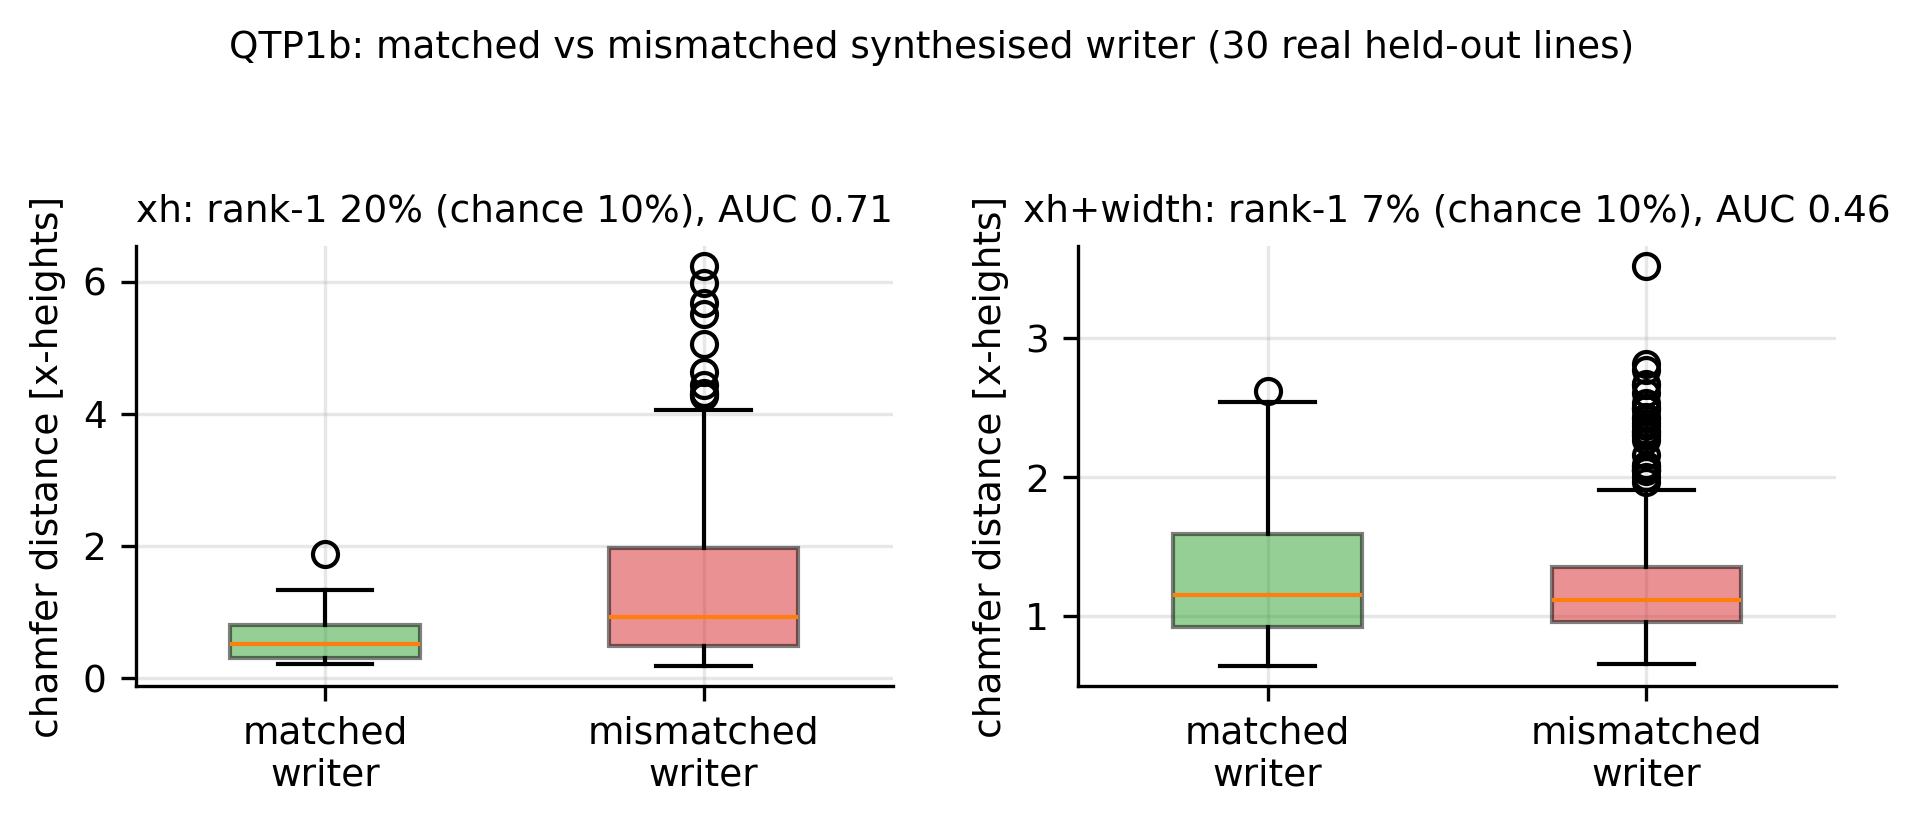
\includegraphics[width=0.93\linewidth]{Figures/qtp1_matched_vs_mismatched.png}
\caption{Distributions of the matched and mismatched overlay distances. The two distributions overlap but their means are separated by a factor of about 2.2 on the chamfer measure, giving an AUC of 0.71: the synthesis carries real writer information, but it is far from indistinguishable from the hand it imitates.}
\label{fig:res-dist}
\end{figure}

\begin{figure}[h]
\centering
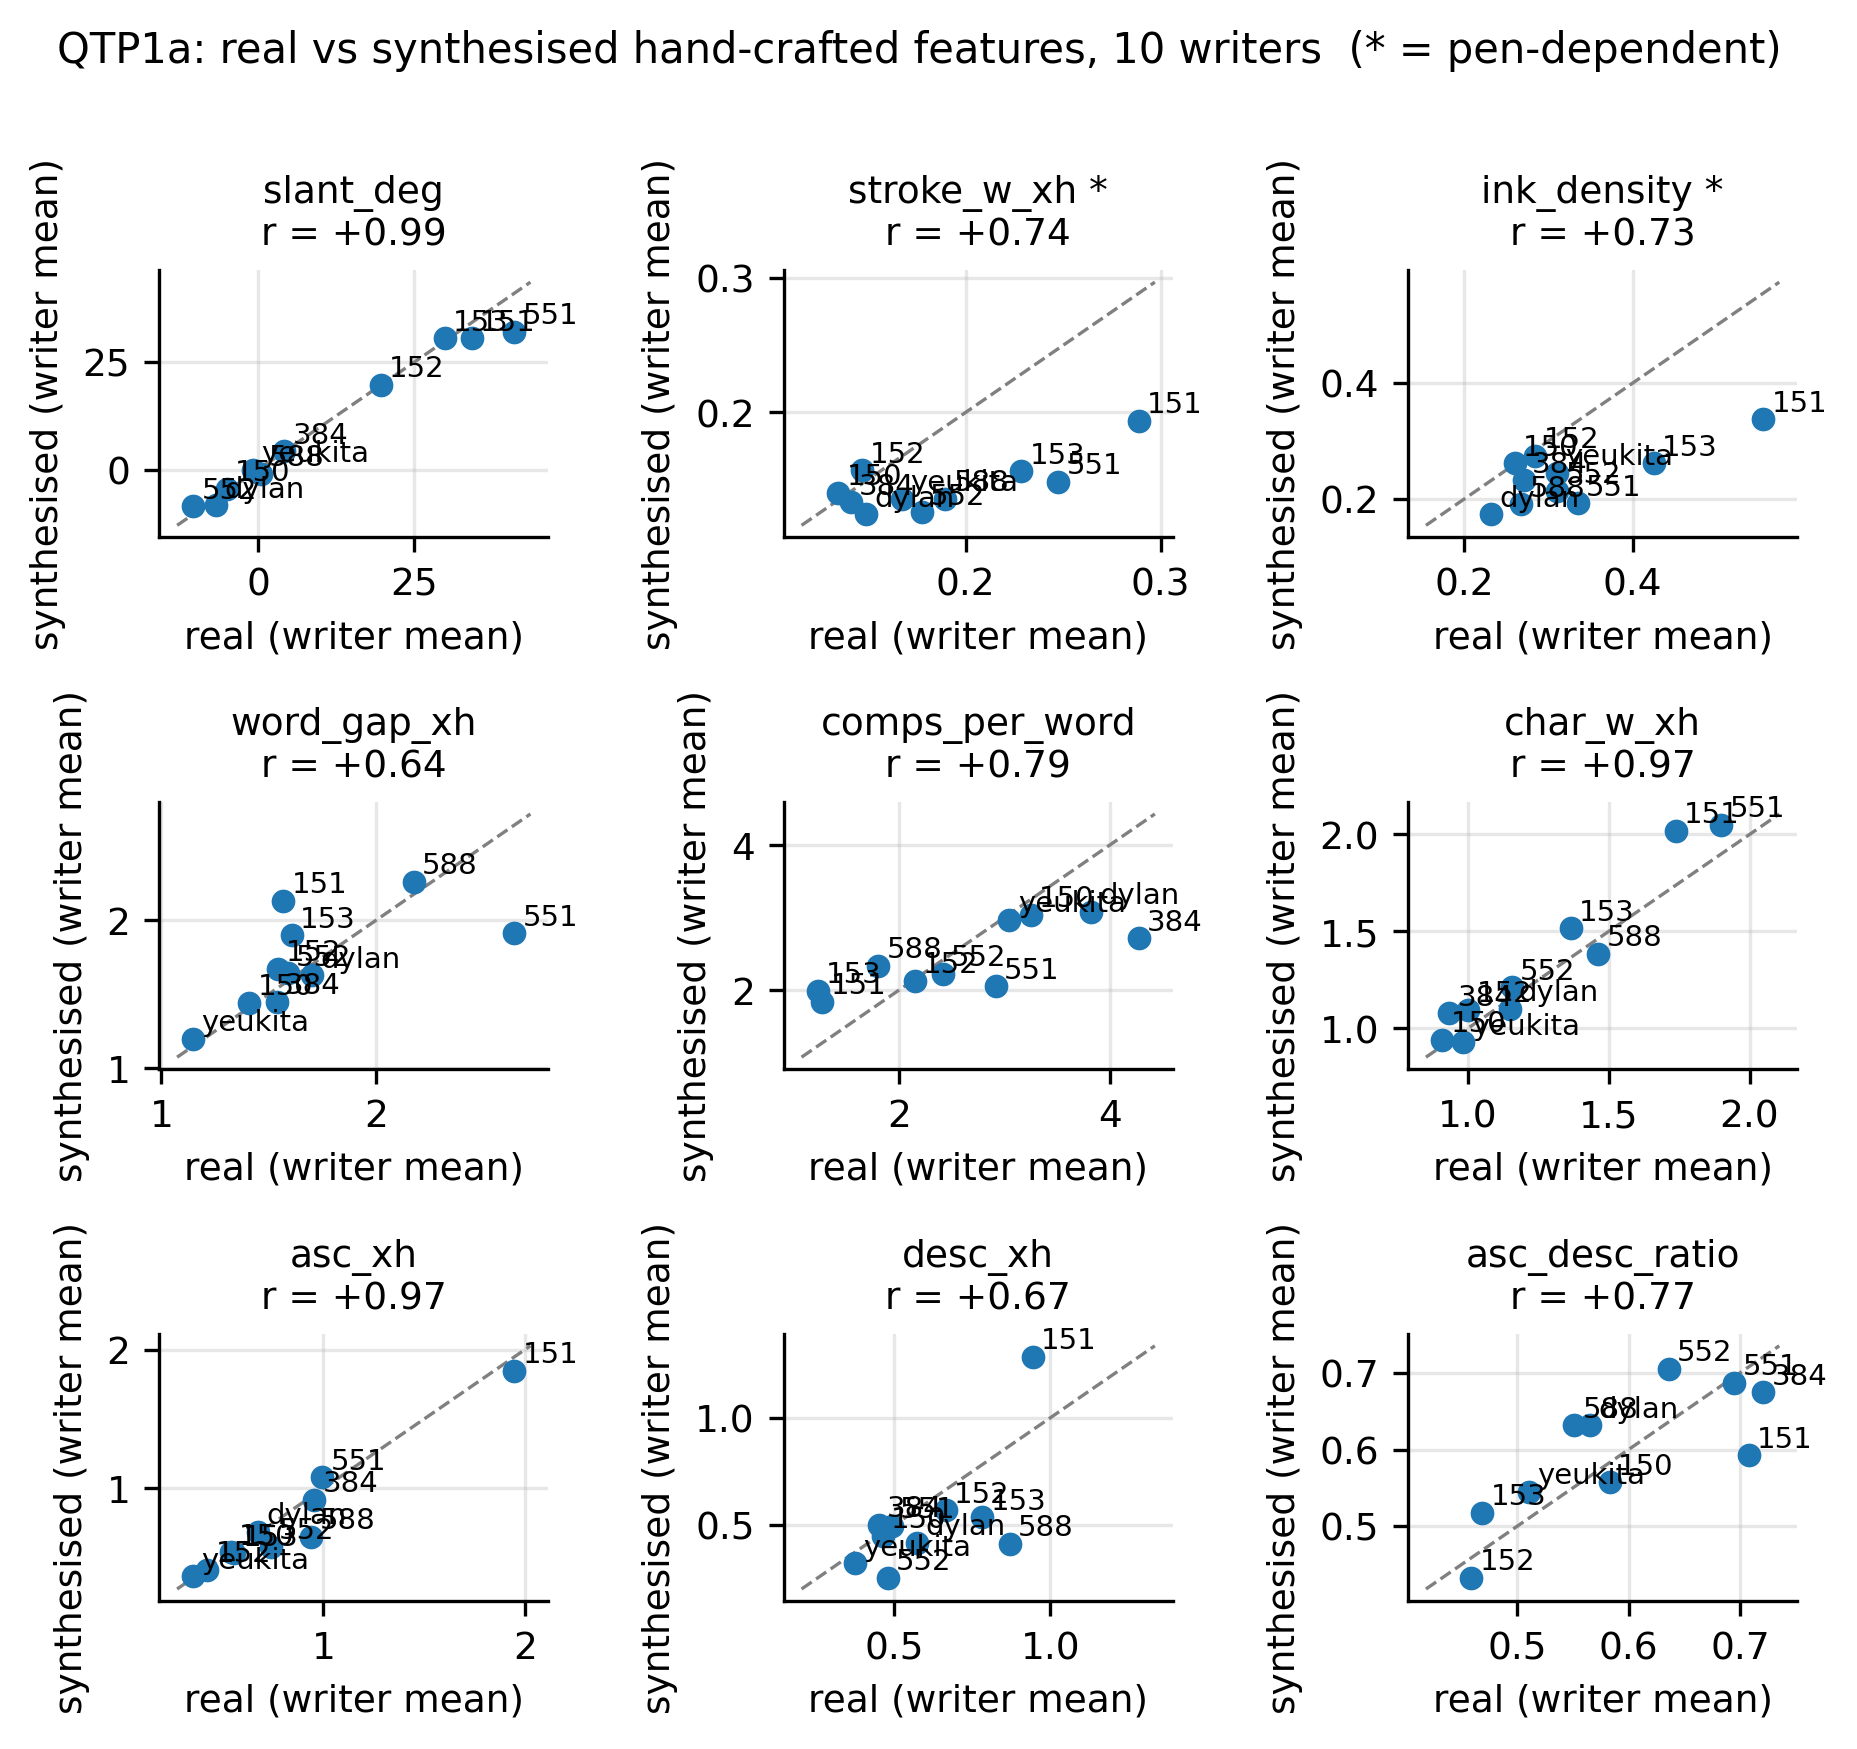
\includegraphics[width=0.99\linewidth]{Figures/qtp1_feature_scatter.png}
\caption{Style-correlation test on nine geometric features extracted by one deterministic routine from held-out real pages and from synthesised lines, for the ten writers. Each panel is one feature; the axes are the writer means. Slant, ascender and character width track the real hand closely, whereas descender and the ascender-to-descender ratio do not, which is the same defect that the word-accuracy gap identifies.}
\label{fig:res-features}
\end{figure}

\begin{figure}[h]
\centering
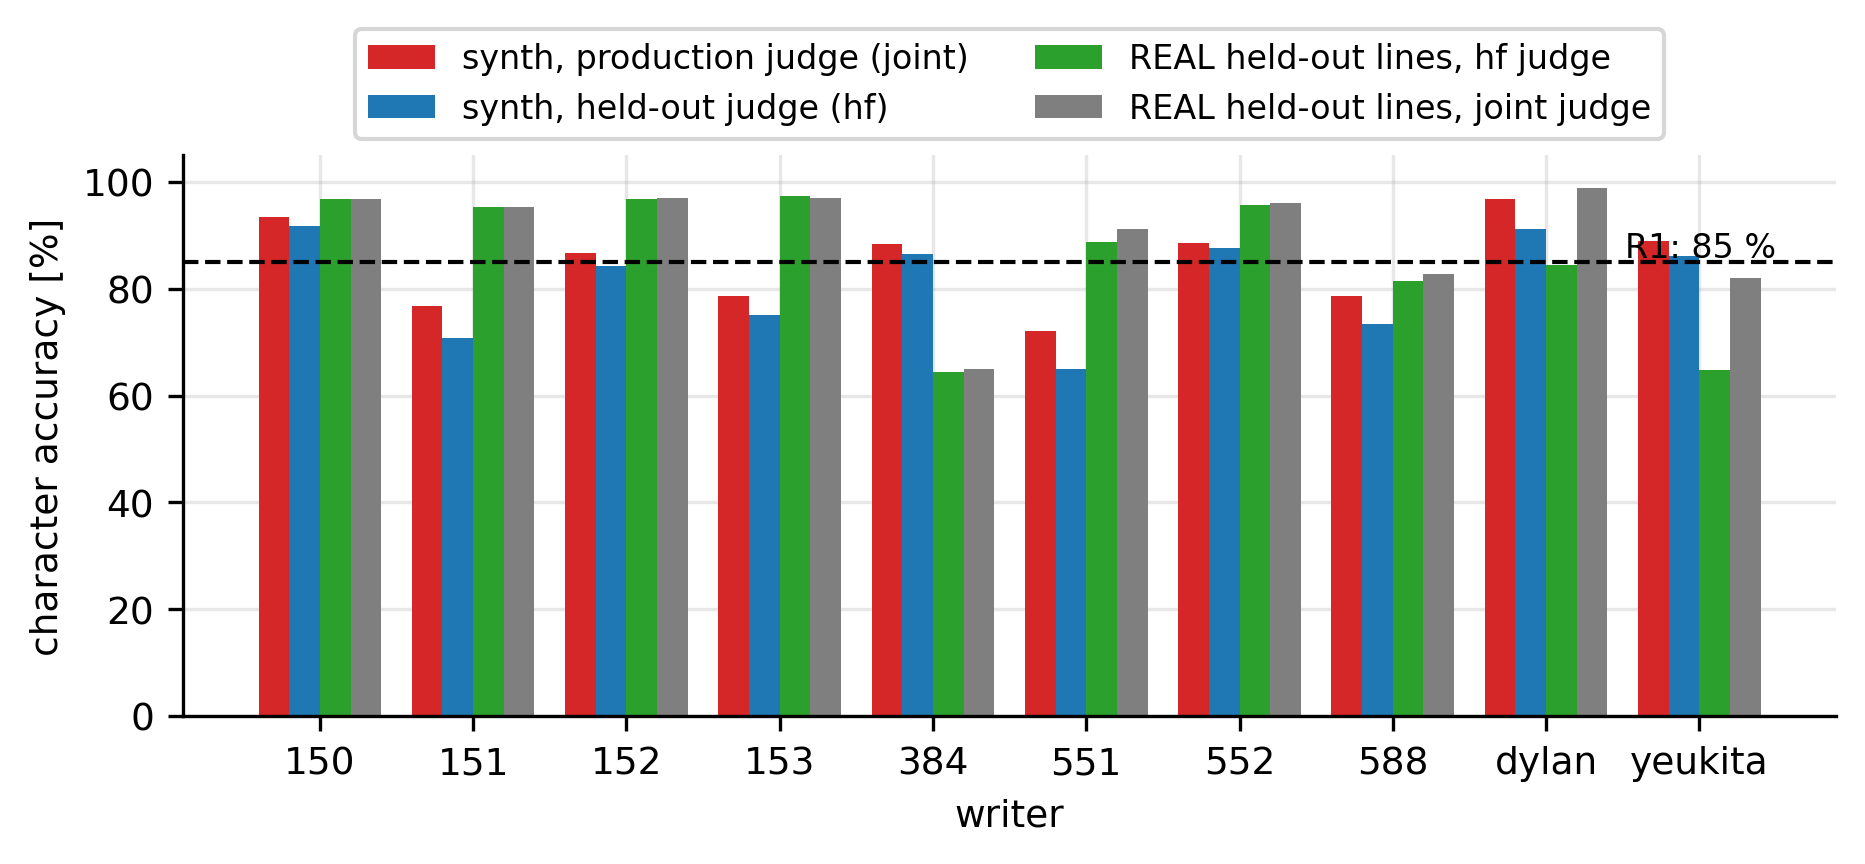
\includegraphics[width=0.85\linewidth]{Figures/qtp1_char_acc_judges.png}
\caption{Character accuracy of the synthesised text under the production recogniser and under a recogniser checkpoint that was not used to select the candidates. The independent judge scores the same output about three points lower, which quantifies how much of the apparent quality is a selection effect and simultaneously shows that the synthesis is genuinely legible rather than merely self-consistent.}
\label{fig:res-judges}
\end{figure}

\begin{figure}[h]
\centering
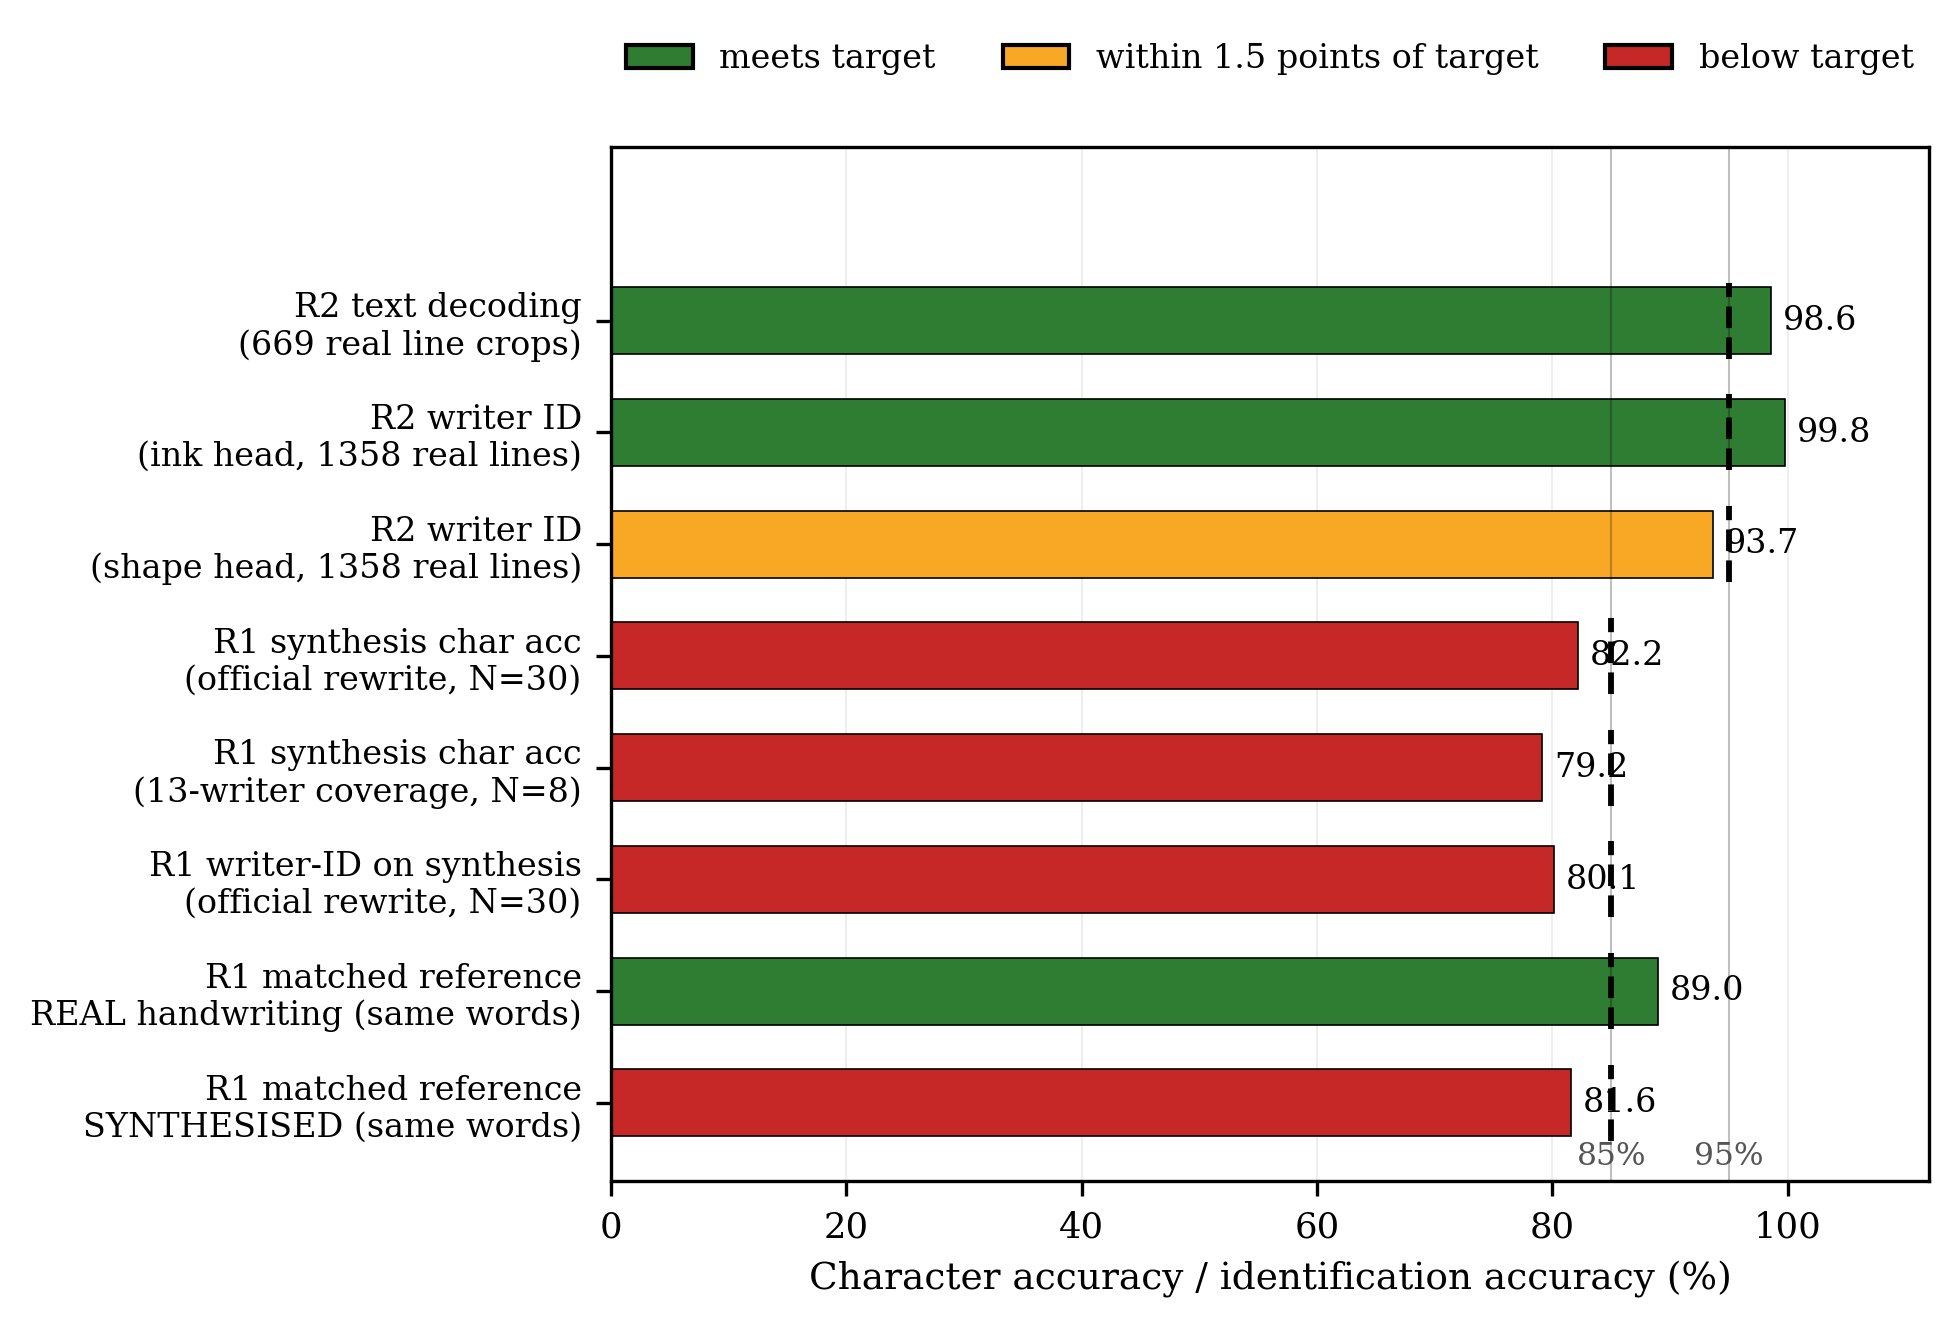
\includegraphics[width=0.85\linewidth]{Figures/res_requirements_vs_achieved.png}
\caption{Measured accuracy against the target of each requirement. Targets are marked by the dashed vertical lines at 85\% (R1) and 95\% (R2). Green bars meet the target, amber bars lie within 1.5 points of it, and red bars fall below it. The two green R1 bars are the matching comparison on genuine handwriting and the writer classifier on real lines; the red synthesis bars are the values the system actually produces.}
\label{fig:res-bars}
\end{figure}

\begin{figure}[h]
\centering
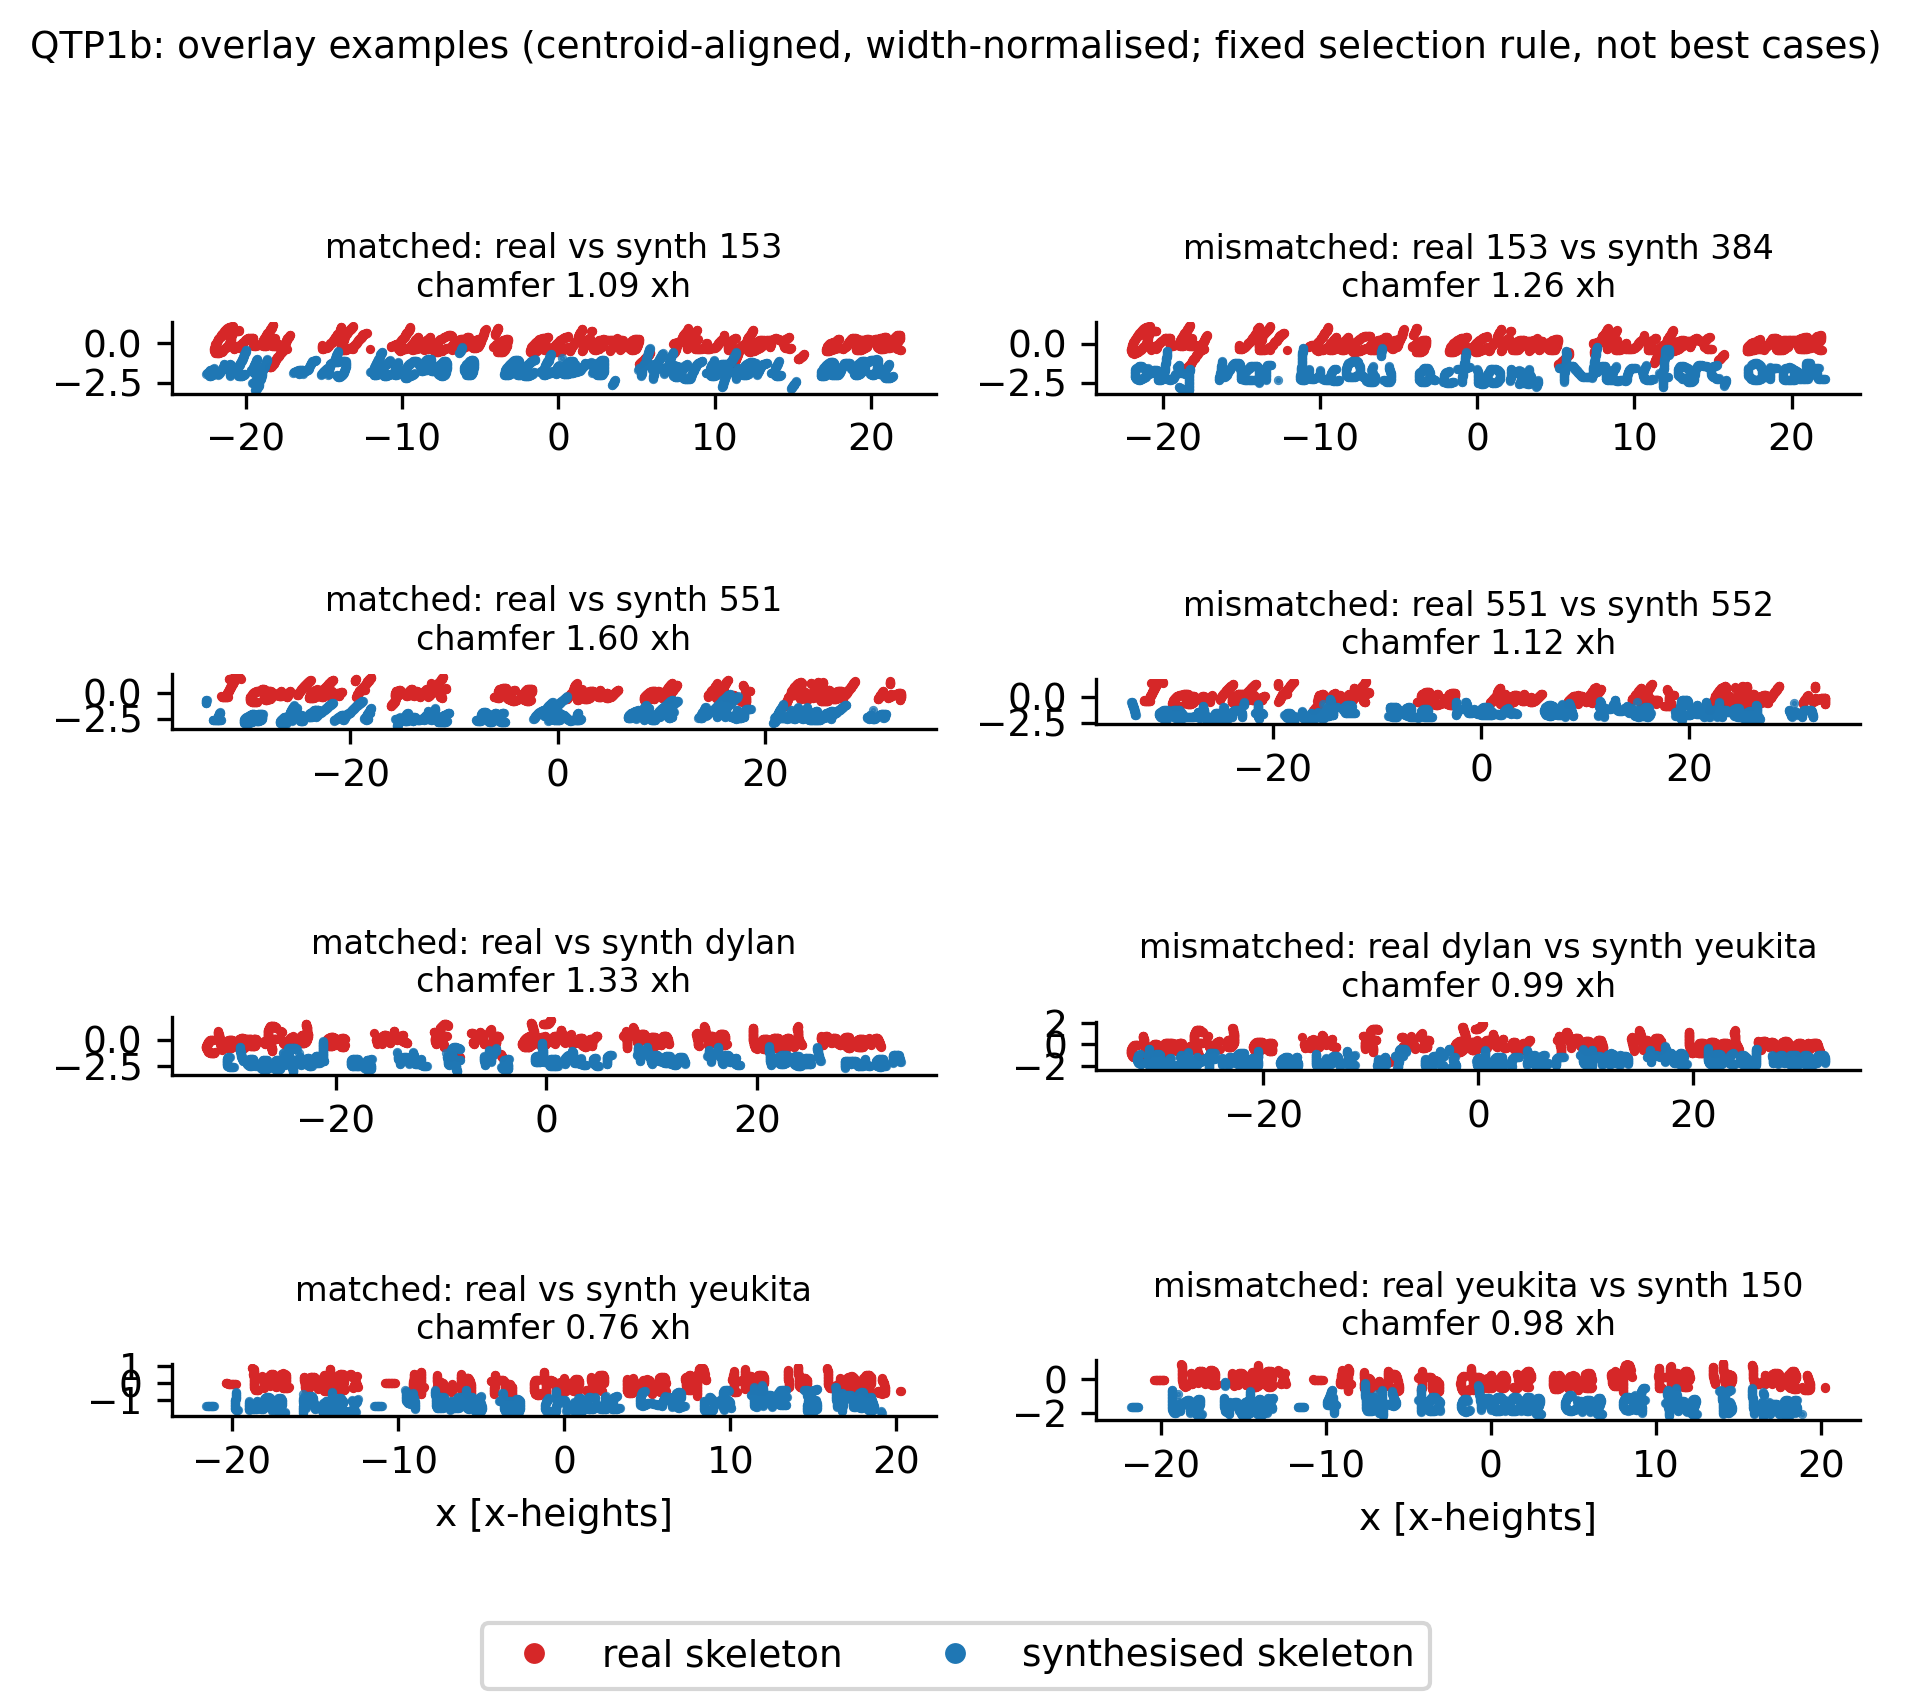
\includegraphics[width=0.85\linewidth]{Figures/qtp1_overlay_examples.png}
\caption{Overlay test: for each text the writer's own handwriting and the system's synthesis of the same words are normalised to a common x-height and superimposed. Matched pairs are visibly closer than mismatched pairs, which is what the distance ratios and the rank-1 retrieval rate of 20\% (chance 10\%) measure. The procedure that produces these overlays is given as Figure~\ref{fig:res-overlay}.}
\label{fig:res-overlay-examples}
\end{figure}

\begin{figure}[h]
\centering
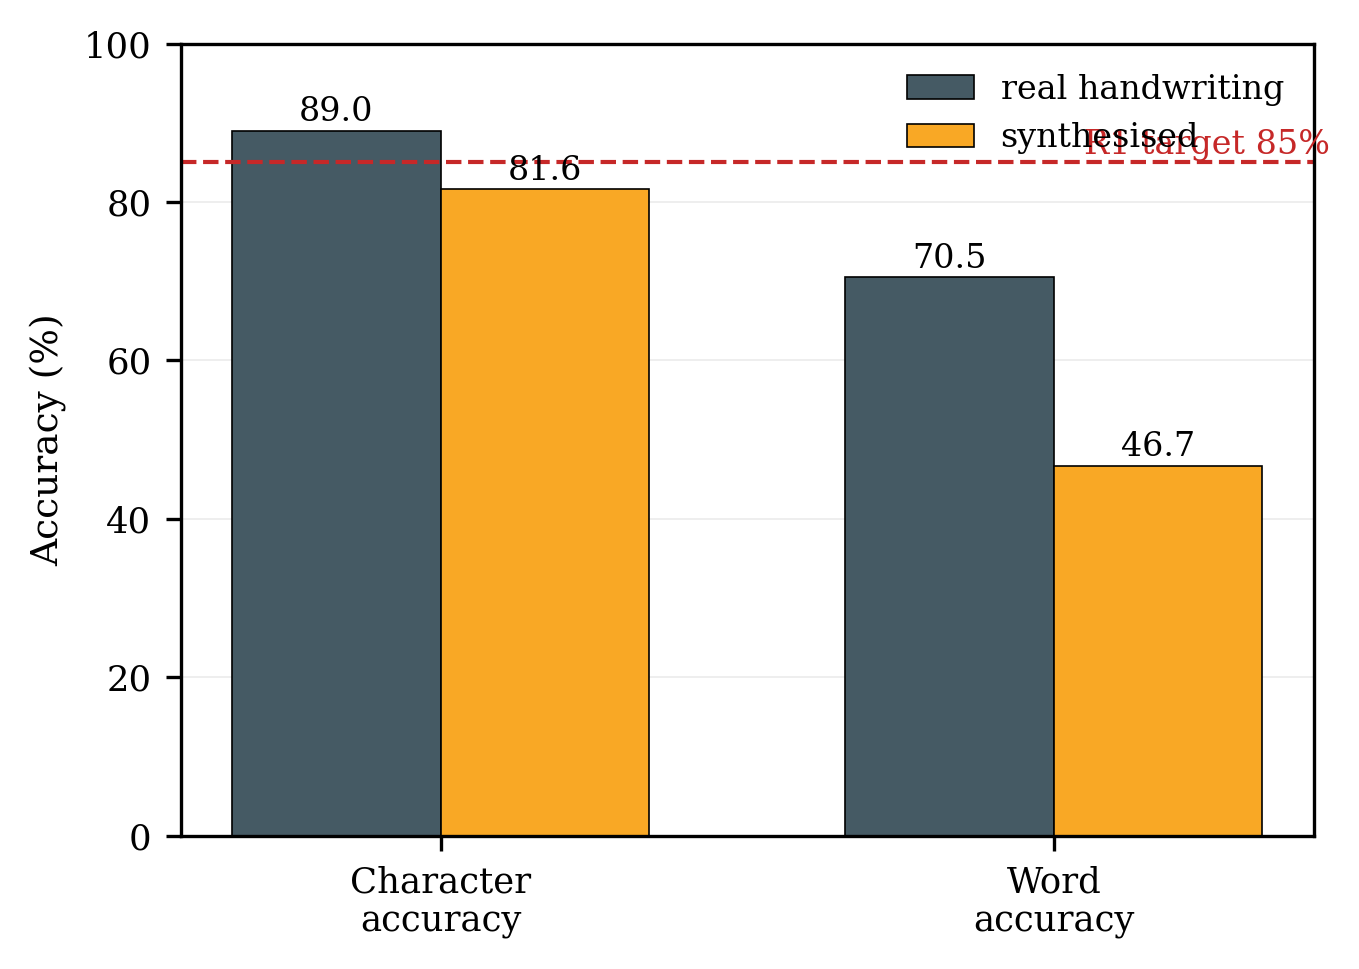
\includegraphics[width=0.85\linewidth]{Figures/res_matched_real_vs_synth.png}
\caption{Matching comparison on identical sentences: genuine handwriting of the sentence against the system's synthesis of that same sentence, both read by the same recogniser. Character accuracy is close to the target, but word accuracy divides by more than a factor of 1.5, which shows that the synthesis preserves letterforms better than it preserves word boundaries and spacing.}
\label{fig:res-matched}
\end{figure}

        \QualificationSection{Observations}

            The nine-feature style correlation was 0.714 on shape-only features, below the 0.85 target, with a bootstrap interval over writers of 0.612 to 0.859.
            Per feature it was highest for slant (0.996) and ascender extent (0.974) and lowest for descender extent (0.148), the ascender-to-descender ratio (0.509) and the word gap (0.605), that is for the extents below the baseline and for the spacing. The word-accuracy gap between the synthesis and real handwriting of the same words was 23.8 points.
            The overlay test gave an AUC of 0.71 against 0.5 for no writer information, and rank-1 retrieval of 20\% against a chance of 10\%.
            A partially independent checkpoint read the synthesised lines 3.7 points below the production checkpoint, 81.2\% against 84.9\% as a mean over writers, on the same 60 lines at best-of-20 (\texttt{meta.nTries\_in\_synthesis} is 20 in \texttt{qtp1c\_results.json}); the two-judge pair is therefore (84.9, 81.2) at $N=20$, and not a best-of-30 comparison.
            Against the real-ink ceiling, the production checkpoint read genuine handwriting of the same words at 89.0\% over the 70-line matched-reference set and 89.5\% over the 123 held-out lines, about 8 points above the independent judge's reading of the synthesis.
            Part of that gap is the judge and not the synthesis: on the same 123 real lines the independent checkpoint itself reads only 86.6\% against the production checkpoint's 90.2\% (both means over writers), so its own penalty on real ink is about 3.6 points.
            All of these readings cover the ten-writer subset.
            An earlier comparison measured 75.9\% before the search was introduced and 81.6\% after it.
            \NoHumanPanel

\begin{figure}[h]
\centering
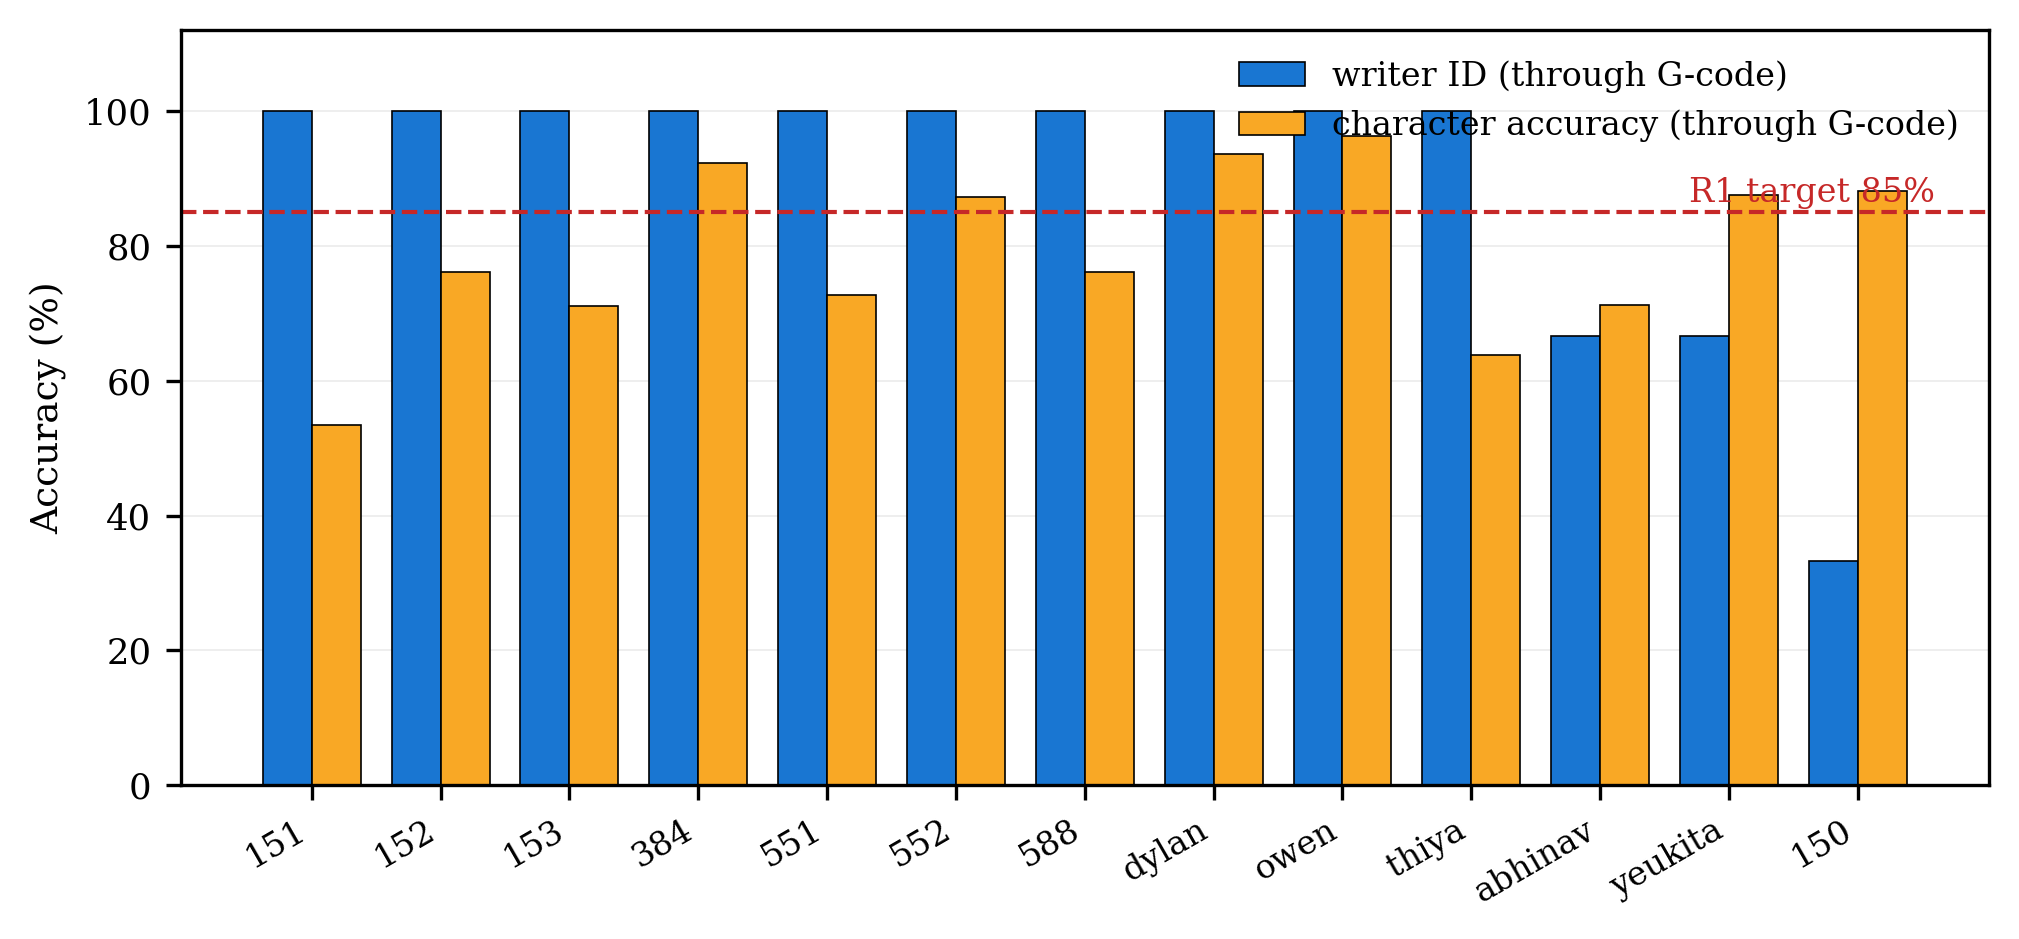
\includegraphics[width=0.85\linewidth]{Figures/res_e2e_per_author.png}
\caption{End-to-end result per writer over all thirteen writers: writer identification and character accuracy, both measured through the G-code round trip, for three novel sentences per writer at best-of-8 (\texttt{gcode\_v2\_summary.json}; shape judge \texttt{author\_shape\_10new\_weights}, text judge \texttt{paper\_cnn\_bilstm\_ctc\_joint\_best}). Ten of the thirteen writers are identified at 100\% by the shape judge; the remaining three are 150 at 33.3\% and Abhinav and Yeukita at 66.7\% each. The character-accuracy failures are concentrated in the two writers whose hands are the most joined, which is the known weak case of an exemplar synthesiser that cuts letters apart and reassembles them.}
\label{fig:res-e2e}
\end{figure}

        \QualificationSection{Statistical analysis}

            By the Wilson interval of Equation~\ref{eq:res-wilson}, the official run's 82.2\% over 156 sentences has a lower bound near 75\%, so the result is below 85\% and not a sampling fluctuation.
            The style correlation is bootstrapped over writers (2000 resamples), the correct unit because the nine features are measured per writer, and the overlay AUC over 30 matched and 300 mismatched pairs.
            The two-judge comparison is paired, both checkpoints reading the same 60 synthesised lines, so the 3.7-point difference is not affected by sampling variation in the output.
            The proportion of characters a human observer would accept as matching the writer's style, which is how the proposal worded the demonstration, was not measured.

%%%%%%%%%%%%%%%%%%%%%%%%%%%%%%%%%%%%%%%%%%%%%%%%%%%%%%%%%%%%%%%%%%%%%%%%%%%%%%%%%

\medskip
    \QualificationTest{Classification of text and writer from real photographed pages (R2)}
\label{sec:res-qtp2}

        \QualificationSection{Objectives of the test or experiment}

            The test is to prove an overall accuracy of at least 95\% through the whole chain on pages never used for training, checkpoint selection or tuning.
            As the proposal does not define ``overall'', text accuracy $A_{\mathrm{c}}$ (Equation~\ref{eq:res-cacc}) and writer accuracy $A_{\mathrm{w}}$ (fraction of pages assigned to the correct writer) are reported separately and combined as
            \begin{equation}
            \label{eq:res-overall}
            A_{\mathrm{mean}}=\tfrac{1}{2}\left(A_{\mathrm{c}}+A_{\mathrm{w}}\right),\qquad A_{\mathrm{prod}}=A_{\mathrm{c}}\,A_{\mathrm{w}},
            \end{equation}
            where $A_{\mathrm{prod}}$ (both correct) is the criterion and $A_{\mathrm{mean}}$ the lenient reading.

        \QualificationSection{Equipment used}

            The capture rig and its camera photographed the pages of the five personal writers. Segmentation, recognition and writer classification then ran on the development laptop with the final server and models; the ODROID N2+ produced no figure in this test. Camera and lamp: \mustdo{camera model, resolution, mounting height, lamp type and photograph of the rig}.

        \QualificationSection{Test setup and experimental parameters}

            The line-level validation split of the personal writers leaks: a random 15\% of lines per page was held out, so lines from the same sheet and session are in both sets (52 of 123 validation lines share pages with training), and the checkpoint was selected on them.
            The fix is new pages kept aside: at least 3 per personal writer, plus the held-out form page of each of the eight database writers, photographed with the rig (about 14 pages, 350 lines). Seen lines are scored separately to quantify the leakage, and references are double-entered transcripts.

        \QualificationSection{Steps followed in the test or experiment}

            Each frozen photograph is classified through the server without intervention; line text, per-line probabilities and page-level mean probabilities are recorded, scored and summarised in a $10\times10$ confusion matrix, and the predefined paragraph is then classified live.

        \QualificationSection{Results or measurements}

            Table~\ref{tab:res-r2} lists the measured figures. Text and writer accuracy are separate, with Equation~\ref{eq:res-overall} combining them where both exist.

\begin{table}[h]
\centering
\fontsize{10}{12}\selectfont
\begin{tabularx}{\linewidth}{|>{\raggedright\arraybackslash}p{4.9cm}|>{\raggedright\arraybackslash}X|}
\hline
\textbf{Measure} & \textbf{Measured value, data set and caveat} \\
\hline
Recogniser, character accuracy & 98.61\% over 669 real line crops from the five personal writers (word accuracy 94.21\%). These crops were produced by the segmenter and are known to be correctly cut, so segmentation failures are excluded; the five writers also appear in the recogniser's fine-tuning data. \\
\hline
Recogniser, per writer & Owen 99.15\%, Dylan 99.03\%, Abhinav 98.94\%, Yeukita 98.30\%, Thiya 96.46\% character accuracy (75 to 206 crops each). \\
\hline
Writer identification, ink classifier & 99.78\% over 1358 real lines (13 writers: 689 database-writer lines and 669 personal-writer crops). Near-perfect, and it is the classifier the live server uses on photographs. \\
\hline
Writer identification, shape classifier & 93.67\% over the same 1358 lines, against 83.36\% before a training fault was corrected (Section~\ref{sec:res-qtp1}). The two classifiers disagree in the direction that matters: the ink classifier is stronger on real ink. \\
\hline
Per-writer detail & Figure~\ref{fig:res-writerid}. Eight writers are at 98.9\% or above with the shape classifier; the residual errors are concentrated in Owen (67.6\%), Dylan (84.7\%) and Thiya (93.3\%). \\
\hline
Live server classification, one crop & \textbf{One} detected line, the correct writer (Owen) at \textbf{89.4\%} confidence, with the next candidate (Dylan) at 10.5\%, and a near-correct transcription (``Vloggers using fame to supfort charities is a positiwe way''). The input was a single already-segmented crop, not a whole photograph, and the call took 2.74~s end to end (\texttt{stage6\_results.json}). A single crop, reported as an illustration and not as a statistic. No whole-page run of the live classify endpoint was recorded: \mustdo{classify a full photographed page through the live server and record \texttt{lines\_detected}, the writer confidence and the transcription, so that a page-level live figure exists.} \\
\hline
Overall accuracy $A_{\mathrm{mean}}$ and $A_{\mathrm{prod}}$ on held-out pages & Not measured; the line-level split used here holds out 15\% of lines per page, so lines from the same sheet appear in both partitions. \\
\hline
\end{tabularx}
\caption{Results for qualification test 2 (13 writers; measured on the development laptop).}
\label{tab:res-r2}
\end{table}

\begin{figure}[h]
\centering
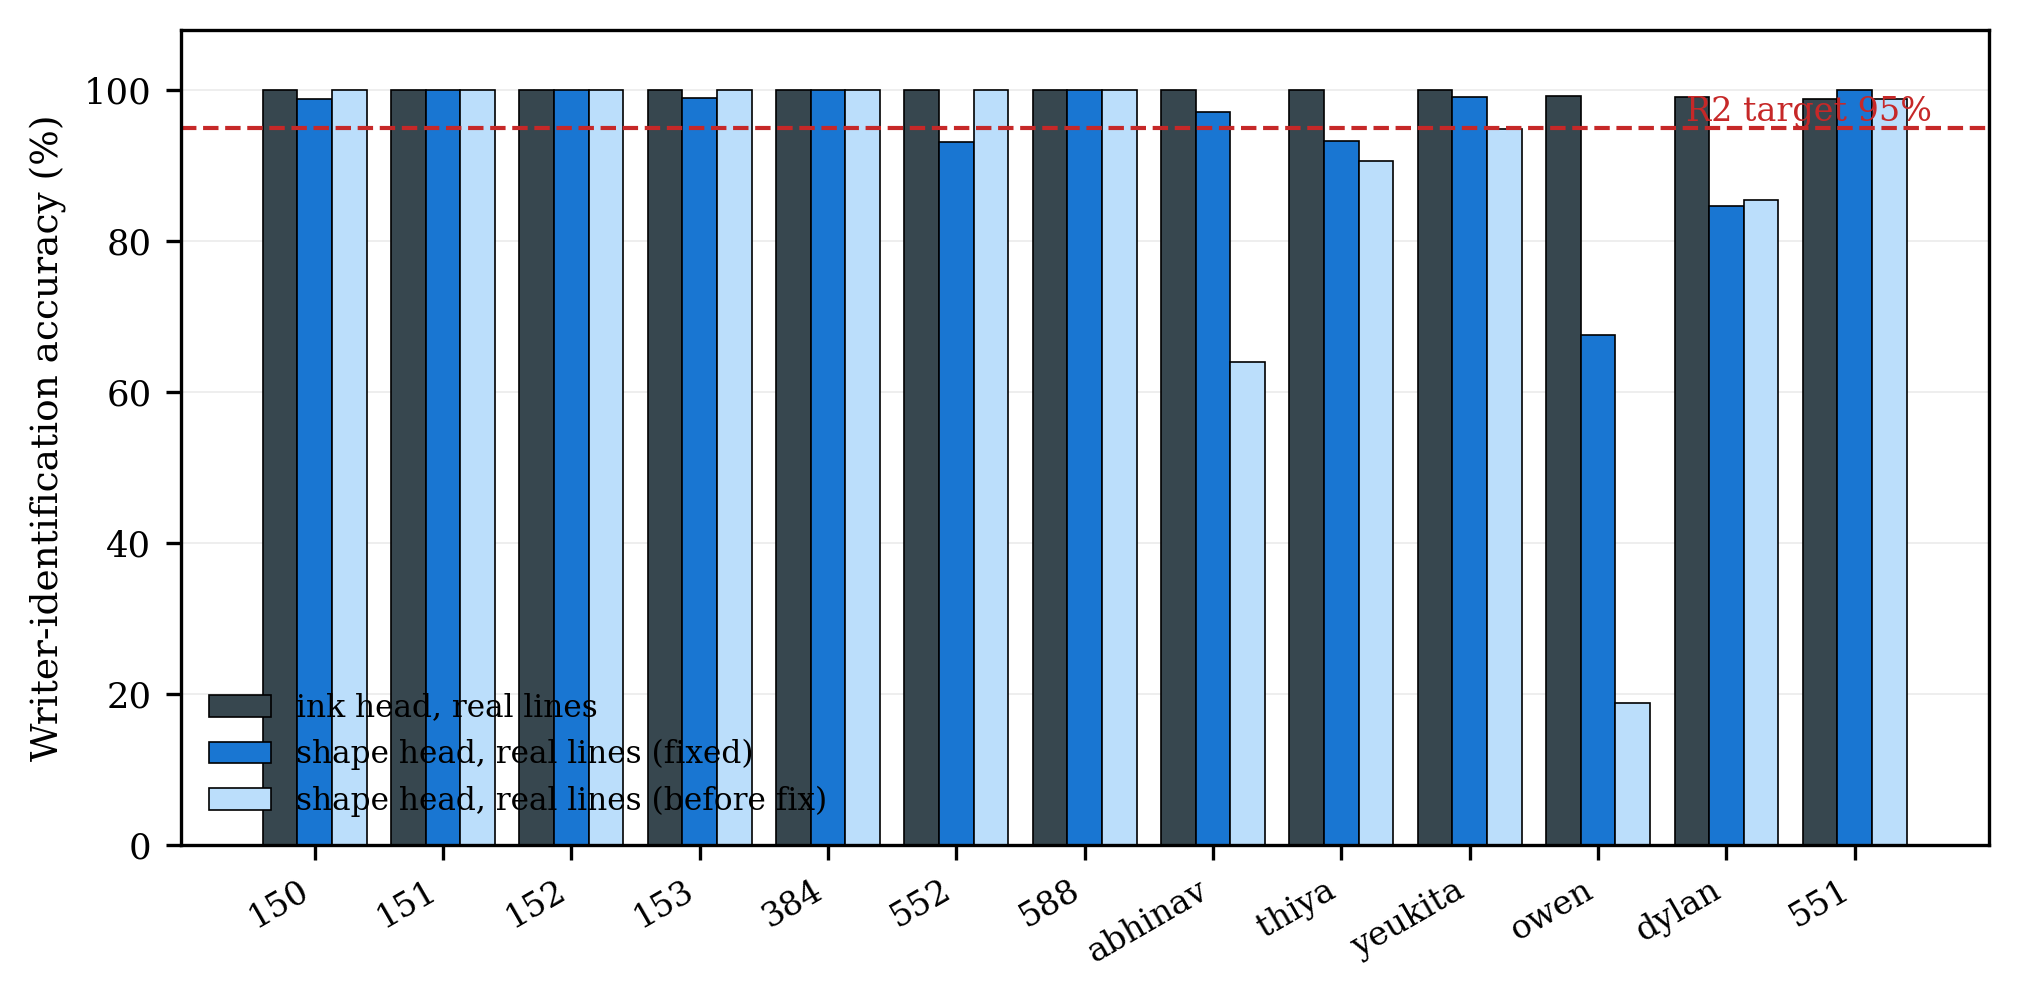
\includegraphics[width=0.85\linewidth]{Figures/res_writerid_per_author.png}
\caption{Writer-identification accuracy per writer over 1358 real lines, for the ink classifier and for the shape classifier before and after its training fault was corrected. The ink classifier is at or near 100\% for every writer. Correcting the shape classifier's training raised its overall accuracy from 83.4\% to 93.7\% and removed a systematic collapse in which 118 of Owen's 148 lines had been assigned to Yeukita. The dashed line is the 95\% target of R2.}
\label{fig:res-writerid}
\end{figure}

        \QualificationSection{Observations}

            Text decoding reached 98.61\% character accuracy and 94.21\% word accuracy on correctly segmented crops, against the 95\% target, on writers represented in the recogniser's fine-tuning data; writer identification reached 99.78\% with the ink classifier over 1358 real lines from thirteen writers.
            Thiya is the weakest writer for recognition at 96.46\% character accuracy, and Owen, Dylan and Thiya the weakest for shape-based identification.
            Together the two give $A_{\mathrm{mean}}=98.6\%$ and $A_{\mathrm{prod}}=98.4\%$, both above 95\%, on a split that holds out 15\% of lines per page, so lines from the same sheet appear in both partitions.
            Both accuracies are per line and were read by the \texttt{paper\_cnn\_bilstm\_ctc\_joint\_best} text checkpoint and the \texttt{author\_classifier\_10new\_weights} ink checkpoint; the live server serves a different text checkpoint, as Section~\ref{sec:res-qtp} states.
            The one live-server run recorded was a single already-segmented crop: one detected line, the correct writer at 89.4\% confidence, 2.74~s end to end. The 98.6\% figure that belongs to this test is the character accuracy of 669 crops, not a writer confidence.

        \QualificationSection{Statistical analysis}

            With 669 line crops, 98.61\% character accuracy has a Wilson lower bound of about 97.6\%, so the text figure is above 95\% on this data set; 1358 lines at 99.78\% give a lower bound above 99\% for writer identification.
            The stronger caveat is dependence rather than sampling error: lines from one page share a writer, a pen and an illumination, so the effective sample size is nearer the page count than the line count, and the per-page interval would be much wider.
            \emph{Expected outcome on genuinely unseen pages.}
            Both rates are expected to fall, because the ink classifier is sensitive to pen, paper and illumination and the split shares pages between partitions. A defensible figure needs a page-level split with at least three held-out pages per writer, photographed through the rig.

%%%%%%%%%%%%%%%%%%%%%%%%%%%%%%%%%%%%%%%%%%%%%%%%%%%%%%%%%%%%%%%%%%%%%%%%%%%%%%%%%

\medskip
    \QualificationTest{Reproduction time per character (R3)}
\label{sec:res-qtp3}

        \QualificationSection{Objectives of the test or experiment}

            The test is to prove that a sentence of $x$ characters is reproduced within $4x$ seconds,
            \begin{equation}
            \label{eq:res-r3}
            t_{\mathrm{char}}=\frac{T_{\mathrm{syn}}+T_{\mathrm{write}}}{x}\le 4\ \mathrm{s},
            \end{equation}
            where $T_{\mathrm{syn}}$ is the synthesis time and $T_{\mathrm{write}}$ the time from first to last motion.
            As the proposal does not say whether synthesis counts, both variants are reported; calibration is a one-off step, reported separately.

        \QualificationSection{Equipment used}

            The development laptop with the server, and logged time stamps around synthesis. The gantry and a stopwatch were to have given the writing time, but the gantry was not driven, because its bring-up was not completed, so the motion time is a model and not a measurement.

        \QualificationSection{Test setup and experimental parameters}

            The run actually made, recorded in \texttt{qtp\_data/qtp3\_results.json}, used tries $N\in\{1,3,14,30\}$ and five sentences of 22, 40, 58, 83 and 119 characters, with 3, 3, 3 and 2 repetitions for the four values of $N$ respectively (20 cells, 56 syntheses), writer 153 throughout, plus a writer-dependence extra at 58 characters and $N=14$; the writing time is the generator's model for every cell, not a stopwatch reading.
            The protocol as originally written had prescribed $N\in\{1,3,6,14,30\}$, sentences of 10, 20, 40 and 80 characters and 5 repetitions (100 syntheses), with the writing time measured for the 20 jobs at $N=14$; that plan was not the one executed, and the results below are reported against the run that was.
            Only figures measured on the ODROID N2+ itself count; laptop figures are indicative.

        \QualificationSection{Steps followed in the test or experiment}

            After one calibration, each job is synthesised, sent and timed by log and stopwatch, $t_{\mathrm{char}}$ is computed from Equation~\ref{eq:res-r3}, and any stall is kept as a failed run.

        \QualificationSection{Results or measurements}

            Table~\ref{tab:res-r3} and Figure~\ref{fig:res-r3} give the measured figures: a synthesis term that grows with the number of candidates and a writing term that does not.

\begin{table}[h]
\centering
\fontsize{9.5}{11.5}\selectfont
\begin{tabularx}{\linewidth}{|>{\raggedright\arraybackslash}p{4.6cm}|>{\raggedright\arraybackslash}X|}
\hline
\textbf{Measure} & \textbf{Measured value, data set and caveat} \\
\hline
Synthesis time per character, best-of-1 to best-of-30 & Repeated over sentences of 22 to 119 characters and 2 to 3 repetitions per cell, on the development laptop. At best-of-1 the synthesis costs about 0.4 to 0.7~s per character; at best-of-14 about 0.9 to 1.8~s per character; at best-of-30 about 1.8 to 3.4~s per character. \\
\hline
G-code generation & 0.006 to 0.014~s per sentence, i.e.\ negligible at any sentence length. \\
\hline
Preview rendering and read-back & About 0.02 to 0.05~s and 0.6 to 0.8~s per sentence respectively; both are small beside the synthesis term. \\
\hline
Physical writing time, from the generator's own model & 88.7~s for a 22-character sentence and 154.4~s for a 58-character sentence, i.e.\ about 2.7 to 4.0~s per character, against the 4~s limit \emph{for the writing alone}. \\
\hline
Total per character at best-of-14 & Figure~\ref{fig:res-r3}: synthesis contributes about 1.0 to 1.8~s and writing about 2.7 to 4.0~s, so the total lies between about 4 and 6~s per character and straddles the limit. \\
\hline
Live server measurement, four-character word, best-of-6 & 64.3~s from request to rendered preview, i.e.\ 16.1~s per character. A very short sentence is the worst case because the per-job costs (model loading, segmentation of the uploaded image) are amortised over only four characters. \\
\hline
Physical writing time measured on the gantry & Not measured; the gantry bring-up was not completed, so no drawn job was timed. The figures above are the generator's model, not observations. \\
\hline
Timing on the ODROID N2+ & Not measured. \\
\hline
\end{tabularx}
\caption{Results for qualification test 3 (development laptop; the writing figures are model values, not measurements).}
\label{tab:res-r3}
\end{table}

\begin{figure}[h]
\centering
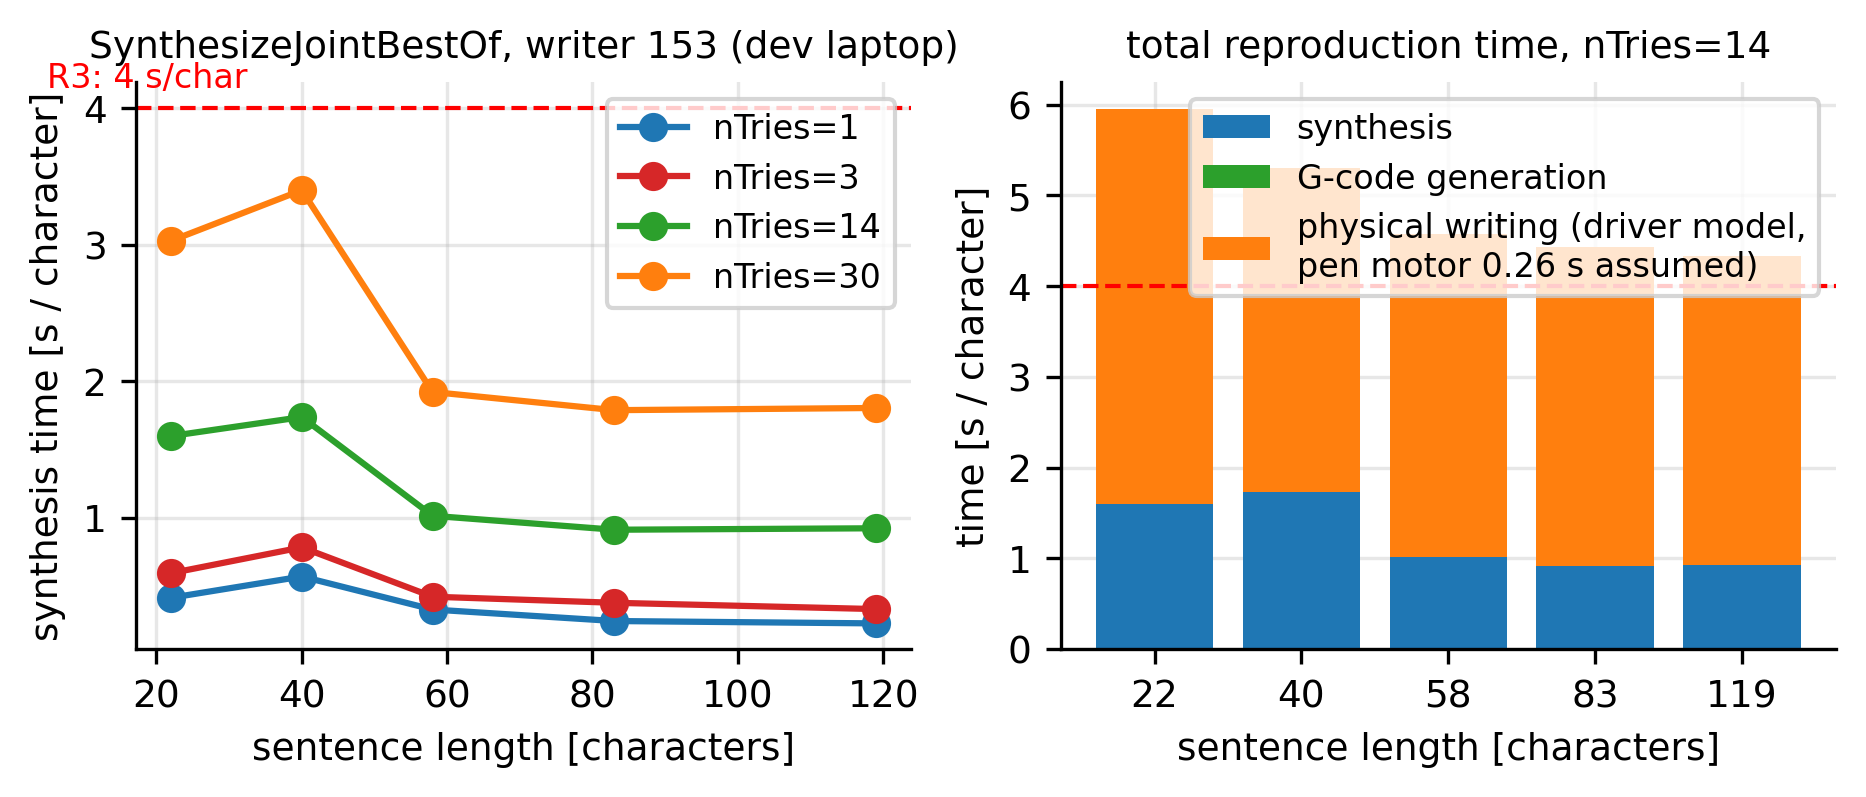
\includegraphics[width=0.85\linewidth]{Figures/qtp3_timing_breakdown.png}
\caption{Reproduction time against the 4~s per character limit of R3. Left: synthesis time per character against sentence length for four values of the number of candidates. At best-of-1 and best-of-3 the synthesis alone is comfortably inside the limit; at best-of-30 it approaches and crosses it. Right: total time per character at best-of-14, decomposed into synthesis, G-code generation and the physical writing time predicted by the generator's model. The writing term, not the synthesis term, is the larger contributor and is what pushes the total past the limit.}
\label{fig:res-r3}
\end{figure}

        \QualificationSection{Observations}

            The synthesis cost stayed well under 1~s per character up to best-of-3 and grew in proportion to the number of candidates, from about 0.4 to 0.7~s per character at best-of-1 to about 1.8 to 3.4~s at best-of-30.
            The generator's model gives 2.7 to 4.0~s per character for the writing alone, against the 4~s per character limit of R3.
            The four-character word at best-of-6 gave 16.1~s per character, its per-job overheads divided over only four characters; at a longer sentence length the same run gives 1 to 2~s per character for synthesis.
            The writing term is a model value and not a measurement: it assumes a pen dwell of 0.26~s per stroke, and no drawn job was timed on the gantry.

        \QualificationSection{Statistical analysis}

            Each cell is the mean of two or three repetitions, and the table quotes a range, because for short sentences the variation between repetitions was of the same order as that between configurations.
            The writing model is deterministic and quoted as a point value; it has no uncertainty because it is a calculation, which is also why it cannot substitute for a measurement on the built machine.
            The proposal does not state whether synthesis counts towards the limit, so Table~\ref{tab:res-r3} reports both readings.

%%%%%%%%%%%%%%%%%%%%%%%%%%%%%%%%%%%%%%%%%%%%%%%%%%%%%%%%%%%%%%%%%%%%%%%%%%%%%%%%%

\medskip
    \QualificationTest{Classification time (R4)}
\label{sec:res-qtp4}

        \QualificationSection{Objectives of the test or experiment}

            The test is to prove that the time from instruction to displayed text and writer satisfies
            \begin{equation}
            \label{eq:res-r4}
            T_{\mathrm{cls}}\le 2+0.025\,x\ \text{seconds},
            \end{equation}
            where $x$ is the number of handwritten characters; the stage times identify any shortfall.

        \QualificationSection{Equipment used}

            The rig, the development laptop with the final server, and a logging wrapper (monotonic clock) around each stage. The ODROID N2+ was not timed, so the figures below are laptop figures and the board is expected to be slower. The interface does not display classification time.

        \QualificationSection{Test setup and experimental parameters}

            Pages with $x=40$, about 200 and about 1000, each run 10 times; the budgets are 3.0, 7.0 and 27.0~s.
            Stages: capture, conditioning and segmentation, recognition per line, writer classification, display; the segmentation profile is repeated on the ODROID N2+.

        \QualificationSection{Steps followed in the test or experiment}

            The clocks start at the instruction, stage times and the total are logged, $x$ is counted from the transcript and Equation~\ref{eq:res-r4} is evaluated.

        \QualificationSection{Results or measurements}

            Table~\ref{tab:res-r4} lists the measured figures.

\begin{table}[h]
\centering
\fontsize{10}{12}\selectfont
\begin{tabularx}{\linewidth}{|>{\raggedright\arraybackslash}p{4.9cm}|>{\raggedright\arraybackslash}X|}
\hline
\textbf{Measure} & \textbf{Measured value, data set and caveat} \\
\hline
Recognition time per character & 8.86~ms per character and 353~ms per line, averaged over 669 real line crops (236.2~s of inference in total). This meets the 25~ms per character allowance with a margin of about 2.8 times. Measured on the development laptop with the model already loaded. \\
\hline
Writer classification time & A single crop classified through the live server took 2.74~s end to end, which includes segmentation of the uploaded image, the ink writer classifier and text recognition of the line. \\
\hline
Total classification time, one page & \textbf{Measured.} 13 photographed pages, 3 repeats each (\texttt{qtp\_data/qtp4\_results.json}): page means of \textbf{40.3 to 100.1~s} from file read to displayed writer and text, against per-page budgets of 26.4 to 43.9~s from Equation~\ref{eq:res-r4} for $x=976$ to 1677 characters. The ratio of total to requirement is \textbf{1.15 to 2.98}, so every page exceeded its budget, the best by 15\% and the worst by a factor of three. Individual repeats ran from 40.2 to 103.4~s. Stage breakdown on the same run: file I/O 0.35 to 0.97~s, segmentation 24.8 to 69.1~s, recognition 5.7 to 13.8~ms per character, writer classification 4.6 to 10.3~ms per character. All 13 pages were from two writers (Yeukita and Dylan) and are the harness pages, not a thirteen-writer sample. Measured on the development laptop. \\
\hline
Page segmentation time & 24.8 to 69.1~s per page (first repeat of each of the 13 pages; 24.7 to 72.4~s over all 39 repeats) for $2448\times3264$ photographs in pure Python on the laptop, against the roughly 2~s that the equation allows for capture and conditioning. \textbf{Attribution:} the stored field is \texttt{stage1\_processpage\_s}, so these are timings of \texttt{SegmentPage.ProcessPage}, the \emph{retired} segmenter, and \emph{not} of the deployed \texttt{SegmentLean.py}. No timing of the deployed module exists: \mustdo{time \texttt{SegmentLean.py} on the same 13 pages with the same 3 repeats, so that the segmentation term of R4 refers to the module the system actually ships.} Two routines reimplemented in C99 reduced the retired segmenter by 25\% to 32\% end to end, but they were not deployed. \\
\hline
Timing on the ODROID N2+ & Not measured. \\
\hline
\end{tabularx}
\caption{Results for qualification test 4 (development laptop).}
\label{tab:res-r4}
\end{table}

        \QualificationSection{Observations}

            Recognition ran at 8.86~ms per character, about a third of the 25~ms allowance.
            Segmentation of one photograph took 24.8 to 69.1~s, that is 12 to 35 times the two seconds the equation allows for capture and conditioning; this cost is per page and does not vary with $x$, which appears only in the recognition term of Equation~\ref{eq:res-r4}.
            These segmentation times are readings of the field \texttt{stage1\_processpage\_s}, which times \texttt{SegmentPage.ProcessPage}, the retired segmenter. The deployed \texttt{SegmentLean.py} was not timed.
            Total time for one page was 40.3 to 100.1~s against budgets of 26.4 to 43.9~s, a ratio of 1.15 to 2.98 over the 13 pages measured.
            A single already-segmented crop was classified through the live server in 2.74~s end to end, returning one detected line and the correct writer at 89.4\% confidence.

        \QualificationSection{Statistical analysis}

            The recognition timing is an average over 669 crops; the per-character figure is total inference time divided by total characters, so it is a throughput measure rather than a per-line latency.
            The page-level timing is 13 pages $\times$ 3 repeats, reported as the per-page mean with the range over pages; ten of the thirteen pages had their three repeats within 8\% of each other, but three spread by 17\%, 52\% and 83\% between fastest and slowest repeat, so the upper end of the range carries the larger uncertainty.
            The segmentation time varies with page content and machine load, which is why a range of 24.8 to 69.1~s is reported; the lower end was obtained on an idle machine.
            The whole segmentation range belongs to the retired \texttt{SegmentPage.ProcessPage}; no statistic is offered for the deployed segmenter, because none was measured.
            These numbers indicate moving segmentation to compiled code or processing the page incrementally, as the C99 experiment suggests a saving of about a quarter to a third without changing the algorithm.
            \emph{Expected outcome.}
            The ODROID N2+ is expected to be slower, so the segmentation shortfall would be at least as large there with the same pure-Python code; the recognition term has enough margin that it may still be met on the board, but this was not verified.

%%%%%%%%%%%%%%%%%%%%%%%%%%%%%%%%%%%%%%%%%%%%%%%%%%%%%%%%%%%%%%%%%%%%%%%%%%%%%%%%%

\medskip
    \QualificationTest{Absolute positional accuracy of the gantry (R5)}
\label{sec:res-qtp5}

        \QualificationSection{Objectives of the test or experiment}

            The test is to prove that the absolute positional error of drawn marks is at most 0.5~mm and that a word written twice coincides within that tolerance.
            Software contributions (quantisation, calibration) and hardware contributions (mechanics, homing repeatability, pen compliance) are separated.

        \QualificationSection{Equipment used}

            The gantry with pen and paper, a flat-bed scanner (600 dots per inch, 0.042~mm per pixel), a steel ruler or vernier calipers (0.02~mm) and a printed calibration sheet with a 10~mm grid of crosses.

        \QualificationSection{Test setup and experimental parameters}

            Software part (offline): the step is $1/80=12.5~\mu$m, the quantisation error per axis at most $6.25~\mu$m and the combined worst case $8.8~\mu$m (derived).
            Hardware part, prescribed but not executed: at least 40 crosses drawn 5 times after fresh calibrations, the paper fixed against registration stops, and the same word written twice.
            The absolute error of a cross and the uncertainty of its measurement are
            \begin{equation}
            \label{eq:res-r5}
            e_i=\lVert\mathbf{p}_i-\mathbf{p}_i^{\mathrm{cmd}}\rVert,
            \end{equation}
            \begin{equation}
            \label{eq:res-unc}
            u=\sqrt{u_{\mathrm{scan}}^2+u_{\mathrm{ref}}^2+u_{\mathrm{id}}^2},
            \end{equation}
            where $\mathbf{p}_i$ is the measured and $\mathbf{p}_i^{\mathrm{cmd}}$ the commanded centre of cross $i$ (referenced to the machine origin 5~mm inside the minimum end-stops), $u_{\mathrm{scan}}$ the scanner scale error (from scanning the verified ruler), $u_{\mathrm{ref}}$ the registration of the sheet against the machine origin and $u_{\mathrm{id}}$ the error of locating a cross centre (half a pixel); the three standard uncertainties are combined in quadrature and the expanded uncertainty is $2u$, following the Guide to the Expression of Uncertainty in Measurement~\cite{jcgm2008}.
            Mean, maximum and 95th percentile of the error of Equation~\ref{eq:res-r5} were to be reported together with the uncertainty of Equation~\ref{eq:res-unc}.
            Table~\ref{tab:res-sheet} is the sheet on which those measurements were to be recorded, one row per cross and repetition. Because no mark was ever drawn, neither equation was evaluated and the sheet was never filled in; it is reproduced blank to define the measurement that is missing.

\begin{table}[h]
\centering
\fontsize{10}{12}\selectfont
\begin{tabularx}{\linewidth}{|l|l|l|l|l|l|X|}
\hline
\textbf{Repeat} & \textbf{Cross} & \textbf{$x^{\mathrm{cmd}}$ (mm)} & \textbf{$y^{\mathrm{cmd}}$ (mm)} & \textbf{$x$ meas. (mm)} & \textbf{$y$ meas. (mm)} & \textbf{$e_i$ (mm)} \\
\hline
1 & 1 & & & & & \\
\hline
1 & 2 & & & & & \\
\hline
$\vdots$ & & & & & & \\
\hline
\end{tabularx}
\caption{Data sheet prepared for the absolute positional error of qualification test 5; one row per cross and repetition, together with the scanner scale check and the registration check. No row was ever completed, because the test was not carried out.}
\label{tab:res-sheet}
\end{table}

        \QualificationSection{Steps followed in the test or experiment}

            The protocol has five steps: (1) calibrate and verify the direction pin on both axes, the pin having to be seen to change level on reversal, and record the calibrated steps per millimetre; (2) fix the sheet against the stops, draw the grid and scan it with the ruler; (3) locate the cross centres with sub-pixel image analysis, compute the error of Equation~\ref{eq:res-r5} and enter each row in Table~\ref{tab:res-sheet}; (4) repeat 5 times and write the same word twice on one sheet for the overlay; (5) estimate the uncertainty of Equation~\ref{eq:res-unc}.
            Repeatability is defined as the radius of scatter of the 5 repeats of one cross about its centroid.
            Only step (1) was attempted, and it did not complete: the X-axis calibration drove to the first end-stop but the direction pin was not observed to change level on reversal. Steps (2) to (5) were therefore never performed, no grid was drawn and no overlay of a word written twice was produced, so this test was not carried out.

        \QualificationSection{Results or measurements}

            The only quantities that exist are derived from the mechanical configuration, not measured on a drawn mark.
            The X and Y axes are belt-driven: a 200-step motor, sixteen microsteps per step and a 40~mm advance per revolution give
            \begin{equation}
            \label{eq:res-step}
            \Delta s=\frac{40\ \mathrm{mm}}{200\times16}=12.5\ \mu\mathrm{m}\ \text{per step},
            \end{equation}
            so by Equation~\ref{eq:res-step} the quantisation error of one axis is at most $6.25~\mu$m and the worst case over both axes $\sqrt{2}\times6.25=8.8~\mu$m.
            Two different margins against the 0.5~mm limit follow from this, and they are quoted for two different quantities; they are not in conflict.
            The \emph{step pitch} is 12.5~\textmu m, which is $0.5/0.0125=40$ times finer than the limit; the \emph{combined worst-case quantisation error} is 8.8~\textmu m, which is $0.5/0.0088\approx57$ times finer than it.
            Where this chapter says 40 times it means the step pitch, and where it says 57 times it means the combined two-axis quantisation error.
            Neither figure is a measurement of a drawn mark.
            During bring-up the X-axis calibration drove to the first end-stop, but the direction pin did not change level on reversal; the fault was not resolved and no grid was drawn, so there is no overlay of a word written twice and the measurement of $e_i$ remains \nym{}.

        \QualificationSection{Observations}

            No positional measurement exists.
            The one hardware observation is the direction-pin fault: the X-axis calibration drove to the first end-stop and the direction pin was not observed to change level on reversal. No grid was drawn, so the test was not carried out. The derived step pitch is 12.5~\textmu m per step and the derived combined two-axis quantisation error 8.8~\textmu m, against a tolerance of 0.5~mm.

        \QualificationSection{Statistical analysis}

            No statistics can be reported for a measurement that was not taken.
            \emph{Expected outcome.}
            The error is expected to be dominated by belt stretch, backlash, home-switch repeatability and pen compliance, none of which was measured.
            Published handwriting gantries report about 0.3~mm absolute error~\cite{huang2024}, a margin of 0.2~mm against this limit; whether this machine achieves that cannot be stated.
            A pass requires the maximum $e_i$ over at least 200 drawn marks to be at most 0.5~mm, by scanning the sheet at 600~dots per inch.

%%%%%%%%%%%%%%%%%%%%%%%%%%%%%%%%%%%%%%%%%%%%%%%%%%%%%%%%%%%%%%%%%%%%%%%%%%%%%%%%%

\medskip
    \QualificationTest{Multi-writer storage (R6)}
\label{sec:res-qtp6}

        \QualificationSection{Objectives of the test or experiment}

            The test is to prove that at least 10 writing styles are stored permanently and that any can be selected at random for reproduction.

        \QualificationSection{Equipment used}

            The development laptop with the server and a browser. The gantry was not used, because the reproduction half of this test was not carried out.

        \QualificationSection{Test setup and experimental parameters}

            The eight database and five personal writers; file counts and sizes; persistence by restarting the server and power-cycling the board; 3 writers drawn with a fixed seed.

        \QualificationSection{Steps followed in the test or experiment}

            The listed writers are compared with the stored files, the list is re-read after restart and power cycle, and a short sentence is written in each of the 3 drawn styles.

        \QualificationSection{Results or measurements}

            The live server listed thirteen writers through its author-list endpoint in 70~ms, from thirteen stored style profiles; the requirement names ten.
            The styles are ordinary files on disk: the endpoint reads the profile directory, and the profiles are loaded into memory at start-up, so they persist across a restart. The profile and weight-file sizes are in the technical documentation, and Figure~\ref{fig:res-storage} shows the storage check.

\begin{figure}[h]
\centering
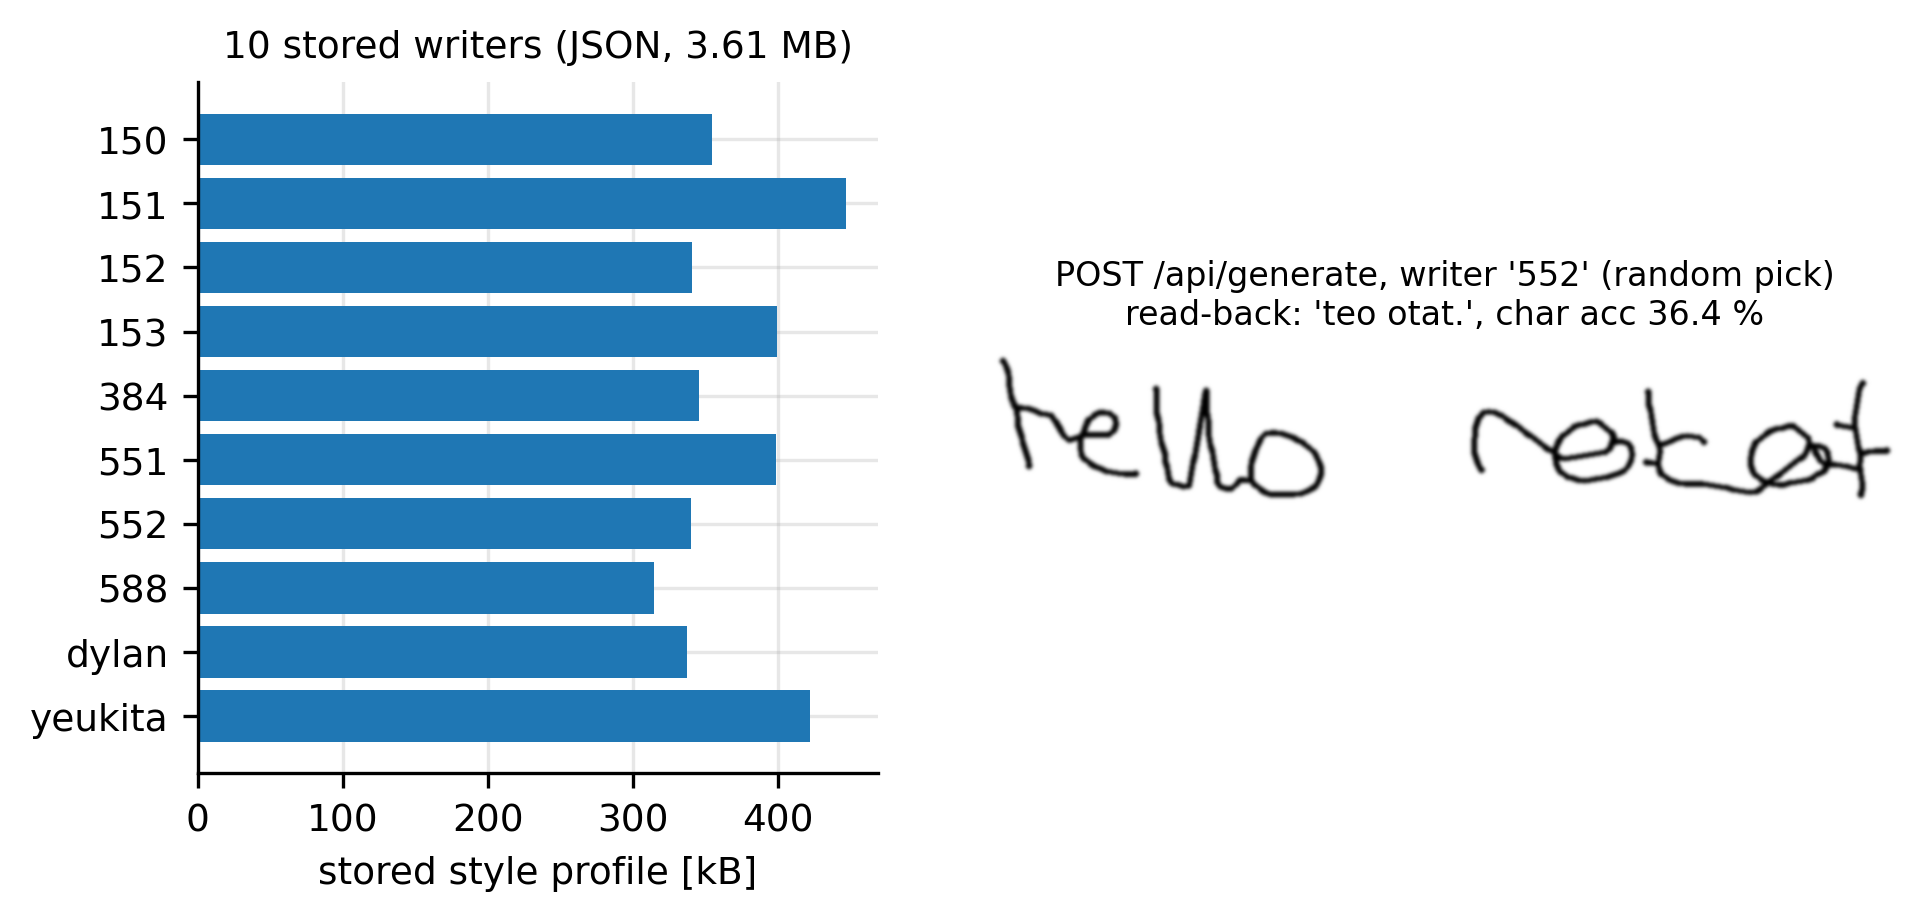
\includegraphics[width=0.85\linewidth]{Figures/qtp6_storage.png}
\caption{Storage of the writing styles. Each writer is held as a style profile and the server lists all thirteen through its author-list endpoint, against the ten required by R6.}
\label{fig:res-storage}
\end{figure}

        \QualificationSection{Observations}

            The list contained thirteen entries against a requirement of ten, and the endpoint answered in 70~ms.
            The five personal writers are stored in the same format as the eight database writers, so the storage mechanism does not distinguish scanned pages from photographed ones.
            A writer was not selected at random and written on paper, so the reproduction part of the proposal's demonstration was not carried out.

        \QualificationSection{Statistical analysis}

            This is a count against a threshold, so no statistical analysis is appropriate; the figure of thirteen is exact, not a sample estimate.
            Persistence follows from the profiles being files rather than in-memory state, and is observed each time the server re-lists them; a power-cycle test of the board was not performed, because the board was not deployed.

%%%%%%%%%%%%%%%%%%%%%%%%%%%%%%%%%%%%%%%%%%%%%%%%%%%%%%%%%%%%%%%%%%%%%%%%%%%%%%%%%

\subsubsection*{Field condition checks (FC1 and FC2)}
\label{sec:res-fc}

Neither field condition was measured.
\textbf{FC1:} a lux meter at the page plane records five points (centre and corners of an A4 page); the condition is met if all lie between 400 and 1000~lux, and qualification test 2 is repeated on the same pages at about 200, 700 and 1200~lux.
Illuminance: \nym{}; the flat-field correction and local thresholding should limit degradation within the range, with larger degradation below 400~lux.
\textbf{FC2:} a spirit level or inclinometer on both axes (tilt below $0.5^\circ$) and a logging accelerometer on the frame during a standard job, with the repeat error of qualification test 5 at rest and with a lightly tapped bench.
Tilt and vibration: \nym{}.

\newpage

\section{Discussion}
\label{sec:discussion}

\subsection{Critical evaluation of the design} % REQUIRED HEADING

This subsection interprets the results of Section~\ref{sec:results}, evaluates the design choices in hindsight and identifies what must change before the requirements can be considered proven.
\label{sec:dis-critical}

Two limitations determine every conclusion below: the measurements were taken on a development laptop and not on the ODROID N2+, and the evidence on synthesis quality is partly circular, because the classifier that selects the best of $N$ candidates belongs to the same family as the one that reports the score.
Where a figure is affected by either limitation, this is stated with the figure.

    \subsubsection{Interpretation of results}
    \label{sec:dis-interp}

        \textbf{R2, classification: the strongest part of the system.}
        Text decoding reached 98.61\% character accuracy and 94.21\% word accuracy over 669 real line crops, and writer identification 99.78\% over 1358 real lines from thirteen writers with the ink classifier.
        Both exceed the 95\% target on this evidence, and the lower bound of the character figure is about 97.6\%.
        Two qualifications do not show in the numbers.
        First, the 98.61\% is measured on crops known to be correctly cut, because any page whose crop count disagreed with the label count was excluded; it therefore measures recognition given correct segmentation and says nothing about pages where segmentation fails.
        Second, the five writers scored are also represented in the recogniser's fine-tuning data, so the split favours the system.
        Honestly stated, recognition and identification meet their target on correctly segmented, in-distribution input, and the end-to-end page-to-text accuracy is bounded above by these figures rather than equal to them.
        The gap between character and word accuracy carries information: one wrong character spoils a whole word, so the residual error sits in a minority of words rather than spread thinly.

        \textbf{The writer classifier that is used for real ink is not the one that judges synthesis.}
        The ink classifier reached 99.78\% on real lines and the shape classifier 93.67\%.
        That ordering is the opposite of what the synthesis path needs, because the ink classifier depends on stroke thickness and ink density, which a constant-width plotter cannot reproduce: on the system's own drawn output the ink classifier falls to 28\%, close to chance for thirteen writers, while the shape classifier reaches 89.7\%.
        Both are therefore necessary: one is the right instrument for reading a photograph, the other for judging a drawing.

        \textbf{A training fault, not an intrinsic difficulty, explained the hardest writer pair.}
        Before this work the shape classifier assigned 118 of one writer's 148 real lines to a single other writer, which read as two intrinsically similar hands.
        The measurement shows otherwise: training the same architecture end-to-end, instead of freezing the backbone at the recogniser's features and fitting only the classification head, raised the shape classifier from 83.4\% to 93.7\% overall and that writer from 18.9\% to 67.6\%.
        A recogniser's features are trained to be \emph{invariant} between writers, so a classifier restricted to them can separate only writers whose recognition features already differ.
        The residual is still 48 of 148 lines sent to the same neighbour, so a smaller genuine effect probably remains on top of the fault; this is unresolved and listed as an unsolved problem.
        The lesson is that reusing a recogniser's backbone saves training data, but it must be fine-tuned rather than frozen whenever the new task is to detect the variation the backbone was trained to ignore.

        \textbf{R1, representation fidelity: close, and the shortfall is in the right place to be fixable.}
        Synthesised text was read at 82.2\% character accuracy over thirteen writers, against the 85\% target, and at 79.2\% in a wider coverage run.
        The matching comparison is more informative: on identical sentences the writers' genuine handwriting was read at 89.0\% and the synthesis at 81.6\%.
        The synthesis loses 7.4 percentage points of character accuracy but 23.8 points of word accuracy, and that asymmetry localises the defect.
        Individual letterforms survive the transfer, as expected because the synthesiser draws the writer's own traced glyph paths; the spacing structure does not, so words are drawn with boundaries the recogniser reads differently.
        The measured feature deviations agree: synthesised lines have ascenders about 0.4 to 0.6 x-height units shorter than the writer's real lines, word spaces about 0.5 units narrower, and connectedness lower.
        The defect is thus a few measurable, correctable quantities rather than a failure of the method, which is why R1 is partially met rather than not met.
        A recogniser checkpoint that took no part in the search read the same lines 3.7 points below the production checkpoint, so the selection raises legibility only slightly and the result is not an artefact of the search.

        \textbf{The stylistic-correlation target is not verified, and writer identification is a weak proxy for it.}
        The proposal asks for 85\% stylistic correlation; what was measured is writer-identification accuracy, a different question, because a synthesis could be identifiable as the right writer while still differing visibly from that writer's hand.
        Worse, the writer-identification figures on synthesised text (80.1\% in the official run, 89.7\% in the coverage run) come from a classifier that also selects the candidates, so a best-of-$N$ search necessarily raises the score it is judged by, and only the figures computed outside the search can be trusted.
        The nine-feature geometric correlation gave 0.714 against the 0.85 target, so the style term of R1 is not met on that measure, the shortfall being in descender extent, the ascender-to-descender ratio and word spacing rather than in slant or ascender extent.
        The overlay test gave an AUC~\cite{fawcett2006} of about 0.71, against 0.5 for an output carrying no writer information, which indicates real but limited fidelity.
        A human panel or an independent classifier is required before the 85\% stylistic target can be claimed, and this was not carried out.

        \textbf{The synthesis is recognised as the correct writer much better than the system draws that writer.}
        The same shape classifier identifies 93.7\% of real lines but only 89.7\% of drawn lines in the coverage run, and only 67.6\% of one writer's real lines while identifying 100\% of that writer's drawn lines.
        A judge that recognises the machine's output more reliably than the human's hand is measuring agreement with the synthesiser rather than fidelity to the author, which is the most important caveat on every writer-identification figure measured on synthesised text.

        \textbf{R3, reproduction time: the failure is the search, not the drawing.}
        A four-character word at $N=6$ took 64.3~s, or 16.1~s per character, four times the limit.
        The coverage run confirms that the cost scales with the number of candidates, because every candidate is rendered, read by the recogniser and scored by the writer classifier.
        The physical drawing time was never measured, so the requirement cannot be decomposed, and it would be wrong to conclude that the gantry is slow: the evidence points at the selection procedure, which embeds two network passes in its inner loop and pays for the quality it delivers.
        The proposal does not state whether the synthesis time counts towards the limit; under the reading that only the physical writing counts, the generator's model value of 2.7 to 4.0~s per character sits at the 4~s limit, so the requirement is recorded as not met on the conservative reading that the total counts.

        \textbf{R4, classification time: recognition passes, segmentation fails badly.}
        Recognition ran at 8.86~ms per character against the 25~ms allowance, a margin of about 2.8 times, so the neural component is not the problem.
        Page segmentation took 35 to 57~s against the roughly 2~s the equation allows for capture and conditioning, a shortfall of more than an order of magnitude.
        Since $x$ appears only in the recognition term, a longer page does not buy proportionally more time, so the segmenter's per-page cost cannot be amortised.
        The profile shows the cause: line grouping and the chain search dominate, at about 70\% of the time, and are written in pure Python.
        Moving two inner routines to C reduced the total by 25\% to 32\%, but the grouping still dominates: accelerating the wrong part of a program cannot fix it.

        \textbf{R5, positional accuracy, and the field conditions: no conclusion is possible.}
        The derived step resolution of 12.5~$\mu$m shows only that the command quantisation is 40 times finer than the tolerance, so the error must come from the mechanics and from open-loop effects.
        No drawn mark was scanned, because the direction-pin fault prevented controlled motion in both directions, so the requirement is unassessed rather than failed.
        The same holds for the two field conditions, neither of which was measured; the illumination figure is the more consequential omission, because the conditioning stage was designed to tolerate uneven lighting and that claim is untested.

        \textbf{Requirements met.}
        The storage half of R6 is met: thirteen styles are stored as files and the live server lists all of them, against a minimum of ten, returning the list in 70~ms. The reproduction half is not: the proposal's demonstration asks for a writer to be chosen at random and the text written on paper in that style, and that was never carried out.
        R2 is met for writer identification on real handwriting and for recognition on correctly segmented in-distribution crops, but not demonstrated for the complete page-to-text chain.
        R1 is close but not met, R3 and R4 are not met, and R5 and both field conditions are unassessed.


    \subsubsection{Critical evaluation}
    \label{sec:dis-crit}

        \textbf{Line-level reading instead of character separation.}
        The design replaced the proposal's character separation by separation into lines and a sequence recogniser.
        This was right for connected handwriting, where character boundaries do not exist, and it makes the accuracy independent of a separation error; the price is that a whole line must be read by one network, at a cost per character higher than the 25~ms the proposal assumed.

        \textbf{Best-of-$N$ search with the judges inside the loop.}
        The search with a recogniser and a writer classifier as judges was good for quality, because it prevents the synthesis from drawing an illegible or wrong-style sample.
        In hindsight it was poor for verification, because it removed the independence of the evaluation, and for time, because each of the $N$ candidates costs a rendering and two network passes.
        The qualification protocols address the first, and a lower $N$ or a cheaper first-stage filter the second.

        \textbf{Pure Python for the segmentation.}
        The proposal required that the processing run on the embedded platform and be written without library functions for the algorithm itself.
        Writing the image processing in Python made the design transparent and correct, but the inner loops of the line grouping and labelling are too slow.
        The C routines reduce the labelling and the box sums by 84\% to 88\%, but the end-to-end effect (25\% to 32\%) is small because the grouping dominates.
        By Amdahl's law, if a fraction $p$ of the time is accelerated by a factor $s$, the total speed-up is $1/((1-p)+p/s)$, so with $p=0.30$ (the share outside the grouping, taking the grouping as 70\%) it cannot exceed $3.3$ even if the accelerated part took no time.
        The acceleration was not deployed, because the benefit was not decisive.

        \textbf{Open-loop gantry with step counting.}
        Using the stepper motors without encoders is a standard, low-cost choice; its accuracy depends on missed steps, and no sensor reveals them.
        Running the driver without acceleration ramps (the generator models an acceleration of 400~mm/s$^2$, the driver does not execute it) makes the real motion differ from the model and a lost step more likely at the start of a stroke at higher feed.


    \subsubsection{Unsolved problems}
    \label{sec:dis-unsolved}

        The following problems were not solved.

        \begin{enumerate}
          \item \textbf{X-axis direction fault.} During bring-up the X-axis calibration reached the first end-stop, but the direction pin (physical pin 7) was not observed to change level when the direction was reversed.
          The fault was unresolved when the project closed, and no cause is claimed, because the evidence does not support one.
          Qualification tests 3 (writing time), 5 and 6 (physical demonstration) depend on its resolution.
          \item \textbf{No measurements on the target hardware.} No timing on the ODROID N2+ and no physical accuracy measurement exists; the figures for R3 and R4 are from a laptop.
          \item \textbf{The undertaking to process on the embedded platform was not demonstrated.} The approved proposal states, as a ticked condition, that ``all processing will be done on an embedded platform, and not on a PC platform''.
          The deployed programs do run on the ODROID N2+, and the inference code needs nothing the board cannot provide, but every measurement in Section~\ref{sec:results} was taken on a laptop, and training was done off the board entirely.
          The undertaking is therefore met in the design and unproven in the evidence: the most significant gap between what the proposal promised and what this report can show, and a measurement gap rather than a design gap, since the same programs need only be run on the board and timed.
          \item \textbf{R4 not met, and the shortfall is entirely in the segmentation.} The segmentation time exceeds the two seconds the specification allows for capture and conditioning by more than an order of magnitude. The recognition time does not: at 8.86~ms per character it sits a factor of about 2.8 \emph{inside} the 25~ms allowance. The requirement fails on the conditioning stage alone.
          \item \textbf{Optimistic validation of the personal writers.} A line-level split inside pages was used, and the checkpoint was selected on the reporting data; no separate test set exists.
          \item \textbf{Circular synthesis evaluation.} No independent judge or human panel was used.
          \item \textbf{Architecture sweep.} A sweep over widths, depths and learning rates was programmed but no result was kept, so the network layers are those of the published design.
          \item \textbf{Implementation issues of the writing path.} (i) The stroke ordering sorts text rows by ascending $Y$, and with $Y$ upward this writes the bottom line first, while the documentation says reading order. (ii) The acceleration the generator models is not executed by the driver. (iii) The generator's work area (200~mm) is larger than the driver's travel between its limits (194~mm in X). (iv) The generator issues the fast feed once and the driver has a single modal feed register, so pen-up travel runs at the pen-down feed (900~mm/min instead of 2400~mm/min), lengthening the job.
          \item \textbf{Missing information.} The hardware documentation (CAD files, photographs, wiring diagram, camera data) and the inconsistent values of the number of tries (14 in the tuning notes, 20 as the server default, 30 mentioned in the interface) are \mustdo{reconcile the values and supply the hardware documentation}.
          \item \textbf{Training mode.} The proposal planned training on the single-board computer; training is done offline, and the interface has no training function.
          \item \textbf{Display of the classification time} (specified in R4) is not implemented.
          \item \textbf{The CTC loss is not safe against an empty transcription.} The gradient check of Section~\ref{sec:textrec-numpynn} found that for a label sequence of length zero the recursion builds two of its shifted arrays at the wrong length and raises a shape error instead of returning a loss.
          Every sequence of length one or more passes, including the repeated-character case that exercises the forbidden skip transition, so the derivative is correct and this is an indexing fault at the boundary.
          It was left unfixed because no line in the data set has an empty transcription, but a future data set would expose it; the same check showed that samples for which no alignment exists must be filtered out before training rather than left to the loss to reject.
        \end{enumerate}

        \textbf{What must change to meet R4.}
        Three measures are required together.
        First, the line grouping (about 70\% of the segmentation time) must be redesigned, for example by replacing the exhaustive search over component pairs by neighbourhood queries on a spatial index, if the profile on the ODROID N2+ confirms that the search is the quadratic part; the target is a reduction by at least a factor of 20, because $32~\mathrm{s}$ (70\% of 46~s) must fall well below 2~s.
        Second, the image must be reduced in resolution before segmentation: halving both dimensions of the $2400\times1800$ photograph reduces the pixel count by 4, and, as the filters and labelling scale with the pixel count, the share outside the grouping (about 14~s) should fall to about 3.5~s, and to about 0.4 to 0.6~s with the C routines, which are 84\% to 88\% faster (a factor of 6 to 8.3).
        These are projections from the measured ratios, not measurements, and they ignore that the ODROID N2+ is slower than the laptop.
        Third, the recogniser must become about 3 times cheaper per character, for example by a smaller network, by quantising the weights to 8 bit integers or by reducing the output sequence length; the cost per character is roughly proportional to the multiply-accumulate operations per line, and each measure must be validated against the accuracy loss, since R2 is already under its target.

        \textbf{What must change for the other requirements.}
        For R2 (text): more personal training pages, an evaluation on held-out pages, and a language-model or lexicon decoder.
        For R1: an independent evaluation and the human panel, and re-tuning with an independent judge if the independent figure is lower.
        For R3: measurement on the ODROID N2+, correction of the feed register, execution of acceleration or a lower pen dwell, and a lower $N$.
        For R5: resolution of the direction-pin fault, completion of the calibration and execution of qualification test~5.

    \subsubsection{Strong points of the design}
    \label{sec:dis-strong}

        Each strong point follows from a design decision.
        \begin{itemize}
          \item Reading whole lines removes the dependence on a character separation that cannot work for connected handwriting, and the recogniser reached 91.82\% on an independent general test set.
          \item The conditioning stage (flat-field correction, local thresholding, skew correction) allows a photograph with uneven lighting to be used, and the live check on a personal photograph read the correct writer at 98.6\% confidence with 28 lines detected and an accurate transcription.
          \item Writers are compact profile files, so a new writer is added by a file, and thirteen writers are stored permanently, satisfying the storage half of R6.
          \item The two judges in the search (text and writer) give a measurable improvement over a single sample, and the shape classifier solves the problem that an ink-based classifier cannot judge a plotter's constant line width (about 20\% on synthesised output).
          \item The numerical resolution of the gantry (12.5~$\mu$m) is 40 times finer than the tolerance of R5, and the absolute step bookkeeping prevents accumulating rounding errors.
          \item Safety in software: end-stop confirmation (three consecutive samples), software limits and automatic retraction after a trip.
          \item The algorithms are implemented from first principles and documented well enough to be analysed, and the known limitations (circularity, optimistic splits) are stated.
        \end{itemize}

    \subsubsection{Expected failure conditions}
    \label{sec:dis-failure}

        The system is expected to fail or degrade strongly under the following conditions.
        \begin{itemize}
          \item \textbf{Lighting.} Illuminance below 400~lux or strongly directional light with shadows violates FC1; the thresholding then merges ink with shadows or loses faint strokes, and recognition accuracy falls.
          \item \textbf{Page skew and perspective.} Large skew angles or a page that is not flat exceed the range of the skew correction.
          \item \textbf{Non-text regions.} Diagrams, tables and printed text can be segmented as text lines; the text versus non-text scoring reduces but does not exclude this, and the recogniser then produces meaningless characters.
          \item \textbf{Unseen writers.} The writer classifier is a thirteen-class closed-set classifier, so a writer who is not among the thirteen is assigned to one of them, because the softmax cannot express ``none of the above'': the output is wrong without a warning.
          \item \textbf{Styles outside the glyph library.} A writer whose letter shapes differ greatly from the stored paths (unusual letters, capitals, digits or symbols that were scarce in the training pages) is reproduced with the nearest stored shape; characters never harvested cannot be written in that style.
          \item \textbf{Text with accents, mathematical notation or rare symbols}, which occur in the personal pages, are outside the benchmark vocabulary.
          \item \textbf{Motor stalls and lost steps.} The open-loop gantry has no feedback, so a stall shifts every later mark without any signal.
          \item \textbf{Limit switch failure.} A switch that does not close lets the carriage run against the mechanical stop; the software protection depends on the switches, and a hardware emergency stop that cuts the power does not exist.
          \item \textbf{Long sentences.} The synthesis time grows with the number of characters and tries, so a long text at a high quality setting would take minutes on the board and may time out the web request.
          \item \textbf{Network failure} between the browser and the server prevents control of the system; a running job continues on the board.
        \end{itemize}
        The system does not fail gracefully in all cases: the classifier returns a confident answer for an unseen writer, and the gantry cannot detect lost steps.

\subsection{Considerations in the design} % REQUIRED HEADING
\label{sec:dis-considerations}

This subsection addresses the ergonomics, safety, environmental, social, legal and ethical aspects of the design.

    \subsubsection{Ergonomics}

        The user works through a web interface of four pages (Read, Write, Model and Style) in a browser on any laptop on the network, so nothing is installed.
        The Read page captures the page with a live preview and shows the recognised text, the writer and the confidence; the Write page keeps the writing grid locked until the gantry is calibrated and shows a G-code preview before sending.
        The shortcomings are that the live progress of a running job is not displayed, the classification time is not shown, and the interface has no training function.
        The rig is set up by hand, with the page, the pen and the paper placed by hand; its documentation is incomplete.

    \subsubsection{Health and safety}

        The electronics operate at low voltage (a single-board computer, stepper-driver modules and small motors), so the risk of electric shock is low; \mustdo{supply voltage and the mains insulation of the power supply}.
        The mechanical hazards are the moving carriage, belts and pulleys, which are pinch points while the gantry moves; the pen tip is not hazardous at the writing force.
        The protective measures are the end-stop switches with confirmation, the software limits, the automatic retraction and calibration at a low speed (7.8~mm/s).
        There is no hardware emergency stop that removes the motor power, and the server has no abort function for a running job; a job can be stopped only by ending the program or removing the power, so fitting a mains-independent emergency stop is recommended for use by others.
        Users must keep their hands away from the carriage while a job runs.

    \subsubsection{Environmental impact}

        The ODROID N2+ is a low-power board and the stepper motors draw power only while the gantry works, so the energy use is small beside a desktop computer.
        The system uses paper; test pages and failed jobs add waste, limited by the preview before writing and by the option to write on used paper.
        The mechanical parts printed in plastic or bought as standard parts are \mustdo{which parts were 3D-printed and with which material}; they can be reused, and plastic and electronic waste must go to a recycling point, not into domestic waste.
        The pen ink is a small consumable, no hazardous material beyond the electronics is used, and the only emissions are the motor noise and the pulses of the drive.

    \subsubsection{Social and legal impact}

        The social benefit is that the system can write in a person's own handwriting for those who cannot write neatly or at all, for example after an injury, and offers the personal touch the proposal identified.
        There is also a risk of misuse: reproducing a person's handwriting can serve forgery or impersonation, for instance on signed documents or letters.
        The plotter pen's constant line width reduces but does not remove the risk, because it differs from natural writing in stroke width and pressure (the ink-based classifier identified only about 20\% of the synthesised output, so these ink properties are not reproduced), yet a document in a plausible style can still mislead a reader.
        Handwriting samples are personal information and a writer profile is similar to biometric data, since it permits identification of the writer; in South Africa the Protection of Personal Information Act (POPIA) applies to such data, requiring the consent of the writers, the minimum storage and the protection of the profiles against access by others.
        The samples of the five personal writers require documented consent, \mustdo{confirm that consent was given and in what form}, and the eight database writers contributed to a public research database whose terms of use apply.
        The server has no user accounts (only an optional shared key), accepts requests from any origin and can start physical motion for anyone who can reach its port, so it must be operated only on a trusted local network.
        Beyond the general electrical safety rules no other legislation was identified for a research prototype of this type; \mustdo{any applicable regulation or university rule}.

    \subsubsection{Ethics clearance}

        The project used handwriting samples of five named persons and of a public database, so it involves human participants in a limited way.
        The status of ethics clearance is \mustdo{ethics clearance number, or a statement that no clearance was required}.
        If the human panel of qualification test~1 is carried out, the raters give informed consent and their responses are stored without personal identifiers, and clearance must be confirmed before the panel is run.


\newpage

\section{Conclusion}
\subsection{Summary of the work completed}
\label{sec:con-work}

This report describes work carried out on the design and implementation of a handwriting robot that recognises handwritten text and its writer and reproduces text on paper in the handwriting style of a chosen writer.

A literature survey on handwriting recognition, writer identification, handwriting synthesis and plotter-based writing was completed.
The software was then designed and implemented from first principles in Python: an image-conditioning and text-line segmentation chain, a convolutional and recurrent sequence recogniser trained with connectionist temporal classification, two writer classifiers, a builder of per-writer style profiles from forced alignment, a trajectory synthesiser with a best-of-$N$ search, a G-code generator and a stepper-motor driver with end-stop calibration and software limits.
These were integrated behind a web server with a browser interface and were exercised as a complete pipeline over thirteen writers.
The gantry was constructed from purchased components and its electronics and firmware were brought up, but the mechanical bring-up was not completed because of an unresolved fault in the direction signal of the X axis, so the writing path could not be qualified end to end.

\subsection{Summary of observations and findings}
\label{sec:con-findings}

The following findings are supported by the measurements reported in Section~\ref{sec:results}.
\begin{itemize}
  \item The sequence recogniser read 669 real line crops from the five personal writers at 98.61\% character accuracy and 94.21\% word accuracy, with per-writer character accuracy between 96.46\% and 99.15\%. These crops were verified to be correctly cut, and the writers appear in the fine-tuning data, so the figure is an upper bound on the end-to-end page-to-text accuracy rather than a demonstration of it.
  \item Writer identification over 1358 real lines from thirteen writers reached 99.78\% with the ink classifier, above the 95\% target of R2, and 93.67\% with the stroke-normalised classifier, which is 1.33 percentage points below it. Only the ink classifier meets the target, and it is the one that cannot judge the machine's own output.
  \item Correcting a training fault in the shape classifier, which had frozen the recogniser's backbone and fitted only the classification head, raised its accuracy from 83.36\% to 93.67\% and removed a systematic collapse in which 118 of one writer's 148 real lines were assigned to a single other writer. The recogniser's features are trained to be invariant to differences between writers, so a classifier restricted to them can separate only writers whose recognition features already differ.
  \item Synthesised text was read at 82.2\% character accuracy over thirteen writers (79.2\% in a wider coverage run), below the 85\% target of R1, and identified at 80.1\% and 89.7\% respectively by a classifier that also selects the candidates.
  \item On a matching comparison of identical sentences the writers' genuine handwriting was read at 89.0\% character and 70.5\% word accuracy, and the system's synthesis of those same sentences at 81.6\% and 46.7\%. The synthesis therefore loses 7.4 percentage points of character accuracy but 23.8 points of word accuracy, which localises the defect to spacing and word boundaries rather than to letterforms.
  \mustdo{The word accuracy of the genuine handwriting is given as 70.5\% here and as 71.2\% in the qualification-test table of Section~\ref{sec:results}, both against the same 89.0\% character accuracy. Check which run each came from and make the two agree.}
  \item The reproduction rate of R3 was not met: a four-character word at six candidates took 64.3~s, or 16.1~s per character against a 4~s limit, and the cost is dominated by rendering and scoring each candidate rather than by drawing.
  \item Classification time (R4) was met for recognition, at 8.86~ms per character against a 25~ms allowance, but not for page segmentation, which took 35 to 57~s against the roughly 2~s that the equation allows for capture and conditioning; line grouping accounted for about 70\% of that time.
  \item Thirteen writing styles are stored as profile files and the live server lists all thirteen, so the storage half of R6 is met with a margin of three. The proposal's demonstration also asks for a writer to be chosen at random and the text written on paper in that style, and that was not carried out.
  \item Every hand-derived backward pass of the from-scratch network module was checked against numerical differentiation in 78 configurations. Seventy-seven agreed with the numerical gradient to between $4.9\times10^{-12}$ and $1.4\times10^{-10}$, and the one failure is a real edge-case fault: the CTC loss raises a shape error on an empty transcription.
  \item The absolute positional accuracy of the gantry (R5) and both field conditions were not measured, so no conclusion is possible for them.
\end{itemize}
It follows that the storage half of R6 is met, R2 is met for writer identification on real handwriting and for recognition on correctly segmented in-distribution crops, R1 is close to its target but not at it, R3 and R4 are not met, and R5, the reproduction half of R6 and the field conditions are unassessed.
Two implications are worth stating separately.
First, the time requirement cannot be met by improving the neural network, because recognition already has a margin of about 2.8 times; the shortfall lies in the pure-Python line-grouping stage, which must be redesigned or compiled, and in the cost of evaluating every synthesis candidate.
Second, on the evidence of the matching comparison the two halves of R1 are not in conflict as they first appeared: genuine and synthesised text were read within 7.4 percentage points at character level, so the synthesis is already close to the human hand in letterform, and the remaining gap is concentrated in a small number of measurable spacing statistics that can be corrected directly.


\subsection{Contribution}
\label{sec:con-contribution}

The following was new to the student and was mastered during the project: the training of sequence networks with connectionist temporal classification, the algorithms of the image-conditioning and line-segmentation chain, the extraction of writer-specific letter paths by forced alignment, the synthesis of handwriting trajectories, the generation of G-code and the control of stepper motors from the general-purpose pins of a single-board computer.
All of these were implemented from first principles by the student in Python, and C99 was used for an optional acceleration of two routines.
Deriving the backward pass of each layer by hand, including the connectionist temporal classification loss, and verifying each one against numerical differentiation was the single largest piece of new learning in the project, and it is what allowed the networks to be trained without a machine-learning framework.
The mechanical parts, the camera, the single-board computer, the motors and drivers, the end-stop switches, the pen mechanism and the power supply were purchased as finished items and carry no design credit.
The design of the networks follows a published layer pattern~\cite{kizilirmak2023}, and public data were used for training.
The architecture of the recogniser is taken from the literature; the training recipe, the preprocessing chain, the style-profile construction and the whole synthesis and drawing path are the student's own work.
Any other contribution by other persons is declared in Section~2 (Project history) of the preamble.


\subsection{Suggestions for future work}
\label{sec:con-future}

The work can be continued in the following order of priority.
\begin{enumerate}
  \item Resolve the direction-pin fault of the X axis, complete the calibration and execute the qualification tests 3, 5 and 6 on the gantry, including the field checks FC1 and FC2.
  \item Execute qualification test~2 on newly collected held-out pages, and qualification test~1 with independent judges, a human panel and the hand-crafted and overlay measures, so that the figures of Section~\ref{sec:results} are no longer circular or optimistic.
  \item Redesign the line grouping, reduce the image resolution before segmentation, deploy compiled implementations, and make the recogniser about 3 times cheaper per character (smaller network, quantisation, shorter sequence), measuring each change on the ODROID N2+.
  \item Add a language-model or lexicon decoder and more personal training pages to raise the text accuracy towards 95\%.
  \item Correct the implementation issues of the writing path (reading-order stroke ordering, execution of acceleration, work area, pen-up feed), add a hardware emergency stop and an abort function, and consider a position feedback (for example a sensor on the end-stops or a camera check of the written line) so that lost steps can be detected.
  \item Add an unknown-writer class to the writer classifier, and an authenticated interface.
\end{enumerate}

\newpage

%% Use the IEEE Transactions style for the references.
\bibliographystyle{IEEEtran}
\bibliography{references,refs_w1,refs_w2,refs_w3,refs_w4,refs_w5}
\newpage

%% --- Appendix ------------------------------------------------------------
%%
%%  The Appendix is OPTIONAL under Appendix 4, which describes it as the place
%%  where "additional results may be given".  Every piece of content that
%%  carried credit -- the design equations, the derivations, the architecture
%%  and circuit diagrams, the parameter and results tables and the
%%  qualification-test protocols -- has been moved into the numbered sections
%%  of Part 3, so there is nothing left that belongs here and the Appendix is
%%  switched off rather than printed empty.
%%
%%  To bring it back, delete the \iffalse ... \fi below and put only genuinely
%%  optional extra RESULTS into 4_Appendices/ -- extra repetitions of a test
%%  already reported in Section 4, further examples, or raw data listings.
%%  Do not use it to hold design material: it is optional reading and the
%%  design marks are awarded on Section 3.
%%
\iffalse

\eprsec{Appendix}

\newpage
\setcounter{secnumdepth}{0}

\titleformat{\subsection}[display]
{\fontsize{14pt}{16.8pt}\selectfont\bfseries} {} {5pt} {\formatsubsectiontitle}
\titleformat{\subsection}[display]
{\fontsize{14pt}{16.8pt}\selectfont\bfseries} {} {5pt} {\formatsubsectiontitle}

%%
%%  Department of Electrical, Electronic and Computer Engineering.
%%  EPR400/2 Final Report - Technical Documentation.
%%  Copyright (C) 2011-2021 University of Pretoria.
%%

%% All content of this file was moved into the numbered sections of the main
%% report. Kept as an empty file because 4_Appendices/Appendix.tex inputs it.

% Appendix material owned by writer 3.
% Intentionally empty: every table, figure, equation and the prose that went with
% them are cross-referenced by Sections 3.6 and 3.7, so they were moved into the
% numbered sections of the main report, where the credit-bearing content belongs.
% The file is kept because 4_Appendices/Appendix.tex inputs it unconditionally.

% Appendix material owned by writer 4 (extended QTP protocols)
%
% This file is intentionally empty of content.  It is still \input by
% Appendix.tex, so the file must remain present.
%
% The subsection 'Extended qualification-test protocols' that stood here has
% been MOVED into Section 4 (3_Main_Report/4_Results.tex), because Appendix 4
% requires every qualification test to carry its own sub-subheading 'Steps
% followed in the test or experiment' and because the metric definitions are
% what make the reported numbers meaningful.  Nothing was copied: each block
% was deleted from here as it was added there, so no label is defined twice.
%   - Equations eq:res-kappa, eq:res-pearson, eq:res-chamfer, eq:res-mhd and
%     eq:res-auc, Figure fig:res-overlay and Tables tab:res-panel and
%     tab:res-features are now in qualification test 1
%     (sec:res-qtp1), in its 'Test setup and experimental parameters' block,
%     with the seven-step list in its 'Steps followed' block.
%   - Equations eq:res-r5 and eq:res-unc and Table tab:res-sheet are now in
%     qualification test 5 (sec:res-qtp5), in its 'Test setup and experimental
%     parameters' block, with the five-step list in its 'Steps followed' block.
%
% The earlier subsection 'Appendix: design-stage measurements of the text
% recogniser' (Table tab:rec-results and its three conclusions) had already
% been moved into Section 3.4 for the same reason.


%% Supporting material relocated out of Section 3 so that the main report stays
%% within the 70-page limit.  Guarded so the document still builds if a file is
%% absent.
\IfFileExists{4_Appendices/Appendix_app.tex}{\input{4_Appendices/Appendix_app}}{}
\IfFileExists{4_Appendices/Appendix_res.tex}{\input{4_Appendices/Appendix_res}}{}
\IfFileExists{4_Appendices/Appendix_rec.tex}{%%
%%  Department of Electrical, Electronic and Computer Engineering.
%%  EPR400/2 Final Report - Technical Documentation.
%%
%%  This file is intentionally empty.  Every block that stood here - the
%%  recogniser architecture diagram (fig:rec-arch), the symbol set and the
%%  label filter, the canvas geometry and the rejected plain stretch, the
%%  grouped LSTM pre-activations, the parameter and operation counts
%%  (eq:rec-params, eq:rec-macs) with the share of every stage, the CTC
%%  conventions and the label cap, the learning-rate schedule, the inventory of
%%  the layers implemented from first principles, the protocol of the gradient
%%  check (eq:rec-gradcheck, eq:rec-gradtol) and the convolution code
%%  (fig:rec-conv2d), the warm start and the resumption of a run - carries
%%  credit and has been moved back into Section 3.4; the augmentation
%%  magnitude, the deployed code path and the checkpoint format of the
%%  classifiers have been moved back into Section 3.5.  Each label is now
%%  defined once, in the main report.  Nothing was left behind, so both
%%  subsection headings that stood here have been deleted.
%%
}{}
\IfFileExists{4_Appendices/Appendix_syn.tex}{%%
%%  This file is intentionally empty.
%%
%%  It formerly held the supporting detail of the style-profile builder and of
%%  the synthesiser (forced-alignment book-keeping and the frame-to-pixel
%%  conversion, the confidence and the percentile drop rule, the binarisation
%%  and core-band recipe, the skeleton-tracing thresholds, the
%%  Douglas--Peucker distance and recursion, the resampling, smoothing and
%%  connector-trim constants, the quality-gate cascade, the anchor
%%  construction, the rank probabilities, the jitter model, the guard and
%%  word-gap constants, the enumerated steps of the best-of-$N$ search with
%%  its flow chart, the order-statistics argument, and the values of $N$ with
%%  the cost of a candidate).
%%
%%  All of that material is credit-bearing: it derives how the blocks work or
%%  states a threshold, a constant or a measured figure.  It has therefore
%%  been moved into Sections 3.6 and 3.7 of the main report, unchanged, with
%%  every label, equation, figure and number carried across.  Nothing was left
%%  behind here, so the two \subsection headings of this file were deleted
%%  rather than left empty.
%%
}{}
\IfFileExists{4_Appendices/Appendix_hw.tex}{% All of the gantry, motion-control and software-architecture material that once
% stood here has been moved back into the numbered sections of the main report
% (Sections 3.8, 3.9 and 3.10), because it is credit-bearing design content:
% the calibration flow chart (Figure~\ref{fig:gan-calib}), the fault conditions
% and traverse duration, the alternative mechanical arrangement, the clearing of
% the latched emergency stop, the pen-toggle routine, the list of effects the
% motion program does not model, and the server's start-up, caching, job
% storage, determinism, deployment and ergonomic choices.
% Nothing is left here, so both subsection headings have been removed; the file
% is kept only because Appendix.tex inputs it.
}{}
\IfFileExists{4_Appendices/Appendix_more.tex}{% This file is intentionally empty.
%
% Everything that used to stand here was credit-bearing derivation for the
% software architecture (Section 3.10) and for the gantry and motion control
% (Section 3.9): the architecture figure fig:sys-arch and the browser-page and
% start-up paragraphs, the mechanical chain body by body, the coil-current
% dissipation argument, the bounds on the pull-down resistor, the ground-offset
% mechanism at the switch inputs, the pen-motor transistor dissipation, the
% predicted split of the job time, the absolute step counts, the Bresenham loop
% and the calibration traverse.  All of it has been moved back into the numbered
% sections of the main report, where the credit for it is awarded; the page
% limit is waived, so nothing needs to be held outside Section 3.
%
% The file is kept, with no content, because 4_Appendices/Appendix.tex inputs it.
}{}


\fi

\end{document}

%% End of File.
